% Options for packages loaded elsewhere
\PassOptionsToPackage{unicode}{hyperref}
\PassOptionsToPackage{hyphens}{url}
%
\documentclass[
]{book}
\usepackage{amsmath,amssymb}
\usepackage{lmodern}
\usepackage{iftex}
\ifPDFTeX
  \usepackage[T1]{fontenc}
  \usepackage[utf8]{inputenc}
  \usepackage{textcomp} % provide euro and other symbols
\else % if luatex or xetex
  \usepackage{unicode-math}
  \defaultfontfeatures{Scale=MatchLowercase}
  \defaultfontfeatures[\rmfamily]{Ligatures=TeX,Scale=1}
\fi
% Use upquote if available, for straight quotes in verbatim environments
\IfFileExists{upquote.sty}{\usepackage{upquote}}{}
\IfFileExists{microtype.sty}{% use microtype if available
  \usepackage[]{microtype}
  \UseMicrotypeSet[protrusion]{basicmath} % disable protrusion for tt fonts
}{}
\makeatletter
\@ifundefined{KOMAClassName}{% if non-KOMA class
  \IfFileExists{parskip.sty}{%
    \usepackage{parskip}
  }{% else
    \setlength{\parindent}{0pt}
    \setlength{\parskip}{6pt plus 2pt minus 1pt}}
}{% if KOMA class
  \KOMAoptions{parskip=half}}
\makeatother
\usepackage{xcolor}
\usepackage{color}
\usepackage{fancyvrb}
\newcommand{\VerbBar}{|}
\newcommand{\VERB}{\Verb[commandchars=\\\{\}]}
\DefineVerbatimEnvironment{Highlighting}{Verbatim}{commandchars=\\\{\}}
% Add ',fontsize=\small' for more characters per line
\usepackage{framed}
\definecolor{shadecolor}{RGB}{248,248,248}
\newenvironment{Shaded}{\begin{snugshade}}{\end{snugshade}}
\newcommand{\AlertTok}[1]{\textcolor[rgb]{0.94,0.16,0.16}{#1}}
\newcommand{\AnnotationTok}[1]{\textcolor[rgb]{0.56,0.35,0.01}{\textbf{\textit{#1}}}}
\newcommand{\AttributeTok}[1]{\textcolor[rgb]{0.77,0.63,0.00}{#1}}
\newcommand{\BaseNTok}[1]{\textcolor[rgb]{0.00,0.00,0.81}{#1}}
\newcommand{\BuiltInTok}[1]{#1}
\newcommand{\CharTok}[1]{\textcolor[rgb]{0.31,0.60,0.02}{#1}}
\newcommand{\CommentTok}[1]{\textcolor[rgb]{0.56,0.35,0.01}{\textit{#1}}}
\newcommand{\CommentVarTok}[1]{\textcolor[rgb]{0.56,0.35,0.01}{\textbf{\textit{#1}}}}
\newcommand{\ConstantTok}[1]{\textcolor[rgb]{0.00,0.00,0.00}{#1}}
\newcommand{\ControlFlowTok}[1]{\textcolor[rgb]{0.13,0.29,0.53}{\textbf{#1}}}
\newcommand{\DataTypeTok}[1]{\textcolor[rgb]{0.13,0.29,0.53}{#1}}
\newcommand{\DecValTok}[1]{\textcolor[rgb]{0.00,0.00,0.81}{#1}}
\newcommand{\DocumentationTok}[1]{\textcolor[rgb]{0.56,0.35,0.01}{\textbf{\textit{#1}}}}
\newcommand{\ErrorTok}[1]{\textcolor[rgb]{0.64,0.00,0.00}{\textbf{#1}}}
\newcommand{\ExtensionTok}[1]{#1}
\newcommand{\FloatTok}[1]{\textcolor[rgb]{0.00,0.00,0.81}{#1}}
\newcommand{\FunctionTok}[1]{\textcolor[rgb]{0.00,0.00,0.00}{#1}}
\newcommand{\ImportTok}[1]{#1}
\newcommand{\InformationTok}[1]{\textcolor[rgb]{0.56,0.35,0.01}{\textbf{\textit{#1}}}}
\newcommand{\KeywordTok}[1]{\textcolor[rgb]{0.13,0.29,0.53}{\textbf{#1}}}
\newcommand{\NormalTok}[1]{#1}
\newcommand{\OperatorTok}[1]{\textcolor[rgb]{0.81,0.36,0.00}{\textbf{#1}}}
\newcommand{\OtherTok}[1]{\textcolor[rgb]{0.56,0.35,0.01}{#1}}
\newcommand{\PreprocessorTok}[1]{\textcolor[rgb]{0.56,0.35,0.01}{\textit{#1}}}
\newcommand{\RegionMarkerTok}[1]{#1}
\newcommand{\SpecialCharTok}[1]{\textcolor[rgb]{0.00,0.00,0.00}{#1}}
\newcommand{\SpecialStringTok}[1]{\textcolor[rgb]{0.31,0.60,0.02}{#1}}
\newcommand{\StringTok}[1]{\textcolor[rgb]{0.31,0.60,0.02}{#1}}
\newcommand{\VariableTok}[1]{\textcolor[rgb]{0.00,0.00,0.00}{#1}}
\newcommand{\VerbatimStringTok}[1]{\textcolor[rgb]{0.31,0.60,0.02}{#1}}
\newcommand{\WarningTok}[1]{\textcolor[rgb]{0.56,0.35,0.01}{\textbf{\textit{#1}}}}
\usepackage{longtable,booktabs,array}
\usepackage{calc} % for calculating minipage widths
% Correct order of tables after \paragraph or \subparagraph
\usepackage{etoolbox}
\makeatletter
\patchcmd\longtable{\par}{\if@noskipsec\mbox{}\fi\par}{}{}
\makeatother
% Allow footnotes in longtable head/foot
\IfFileExists{footnotehyper.sty}{\usepackage{footnotehyper}}{\usepackage{footnote}}
\makesavenoteenv{longtable}
\usepackage{graphicx}
\makeatletter
\def\maxwidth{\ifdim\Gin@nat@width>\linewidth\linewidth\else\Gin@nat@width\fi}
\def\maxheight{\ifdim\Gin@nat@height>\textheight\textheight\else\Gin@nat@height\fi}
\makeatother
% Scale images if necessary, so that they will not overflow the page
% margins by default, and it is still possible to overwrite the defaults
% using explicit options in \includegraphics[width, height, ...]{}
\setkeys{Gin}{width=\maxwidth,height=\maxheight,keepaspectratio}
% Set default figure placement to htbp
\makeatletter
\def\fps@figure{htbp}
\makeatother
\setlength{\emergencystretch}{3em} % prevent overfull lines
\providecommand{\tightlist}{%
  \setlength{\itemsep}{0pt}\setlength{\parskip}{0pt}}
\setcounter{secnumdepth}{5}
\usepackage{booktabs}
\usepackage{amsthm}
\usepackage[left=2cm,right=2cm,top=2cm,bottom=2cm]{geometry}
\makeatletter
\def\thm@space@setup{%
  \thm@preskip=8pt plus 2pt minus 4pt
  \thm@postskip=\thm@preskip
}
\makeatother
\ifLuaTeX
  \usepackage{selnolig}  % disable illegal ligatures
\fi
\usepackage[]{natbib}
\bibliographystyle{apalike}
\IfFileExists{bookmark.sty}{\usepackage{bookmark}}{\usepackage{hyperref}}
\IfFileExists{xurl.sty}{\usepackage{xurl}}{} % add URL line breaks if available
\urlstyle{same} % disable monospaced font for URLs
\hypersetup{
  pdftitle={The Datatrain R Bootcamp},
  hidelinks,
  pdfcreator={LaTeX via pandoc}}

\title{The Datatrain R Bootcamp}
\author{}
\date{\vspace{-2.5em}}

\begin{document}
\maketitle

{
\setcounter{tocdepth}{1}
\tableofcontents
}
\hypertarget{welcome}{%
\chapter{Welcome!}\label{welcome}}

\hypertarget{what-this-is-and-what-it-isnt}{%
\section*{What this is, and what it isn't}\label{what-this-is-and-what-it-isnt}}
\addcontentsline{toc}{section}{What this is, and what it isn't}

This is not a textbook or an encyclopedia. This is not a reference manual. It is not exhaustive or comprehensive. We won't mention statistical tests at all. There is almost no theory. In fact, this curriculum is biased, non-representative, and incomplete -- \emph{by design.}

\textbf{So what is this?} This guide is an \emph{accelerator,} an \emph{incubator} designed to guide you along the most direct path from your first line of code to becoming a capable data scientist. Our goal is to help you through the most dangerous period in your data science education: your very first steps. The first three weeks. That is when 99\% percent of people give up on learning to code.

But it doesn't need to be this way. We made this book to reach more than just the 1\%.

We have based our approach on three core premises:

\textbf{Premise 1: We learn best by doing.} Our goal is to get you \emph{doing} data science. We will keep theory and detail to a minimum. We will give you the absolute basics, then offer you exercises and puzzles that motivate you to learn the rest. Then, once you've been \emph{doing} data science for a bit, you soon begin \emph{thinking} like a data scientist. By that, we mean tackling ambiguous problems with persistence, independence, and creative problem solving.

\textbf{Premise 2: We learn best with purpose.} Once you gain comfort with the basic skills, you will be able to start working on real data, for real projects, with real impact. You will start to \emph{care about what you are coding}. And that is when the learning curve \emph{skyrockets} -- because you are motivated, and because you are learning \emph{reactively}, instead of passively. Our goal is to get you to the point of take-off as quickly as possible.

\textbf{Premise 3: A simple toolbox is all you need to build a house.} Once you become comfortable with a few basic coding tools, you can build pretty much anything. The toolbox doesn't need to be that big; if you know how to use your tools well, and if you have enough building supplies (i.e., data), the possibilities are limitless.

\hypertarget{who-this-is-for}{%
\section*{Who this is for}\label{who-this-is-for}}
\addcontentsline{toc}{section}{Who this is for}

The target audience for these tutorials is the \emph{rookie}: the student who \emph{wants} to work with data but has \emph{zero} formal training in programming, computer science, or statistics.

\hypertarget{what-you-will-learn}{%
\section*{What you will learn}\label{what-you-will-learn}}
\addcontentsline{toc}{section}{What you will learn}

\begin{itemize}
\tightlist
\item
  The \textbf{Core theory} unit establishes the conceptual foundations and motivations for this work: what data science is, why it matters, and ethical issues surrounding it: the good, the bad, and the ugly. Don't slog through this all at once. Sprinkle it in here and there. The most important thing, at first, is to start writing code.
\end{itemize}

The next several units comprise a \emph{core} curriculum for tackling data science problems:

\begin{itemize}
\item
  The \textbf{Getting started} unit teaches you how to use \texttt{R} (in \texttt{RStudio}). Here you will add the first and most important tools to your toolbox: working with variables, vectors, dataframes, scripts, and file directories.
\item
  The \textbf{Basic \texttt{R} workflow} unit teaches you how to bring in your own data and work with it in \texttt{R}. You will learn how to produce beautiful plots and how to reorganize, filter, and summarize your datasets.
\end{itemize}

For these first two units, we encourage you to take on these modules one at a time, in the exact order they are presented: we put a lot of thought into what we included in these modules (and what we did not).

\begin{itemize}
\item
  The \textbf{Review exercises} unit provides various puzzles that allow you to apply the basic \texttt{R} skills from the previous unit to fun questions and scenarios. In each of these exercises, questions are arranged in increasing order of difficulty, so that beginners will not feel stuck right out of the gate, nor will experienced coders become bored. This is where you really begin to cut your teeth on real-world data puzzles: figuring out how to use the \texttt{R} tools in your toolbag to tackle an ambiguous problem and deliver an excellent data product.
\item
  The \textbf{Reproducible research} unit equips you with basic tools needed for truly reproducible data science: documenting your research and code with \texttt{Markdown}; weaving together your code and your reporting with \texttt{RMarkdown};
  allowing users to explore the data themselves with an interactive \texttt{Shiny} dashboard or web app; and sharing your code and tracking versions of your code using \texttt{Git}.
\end{itemize}

\hypertarget{who-are-we}{%
\section*{Who are we?}\label{who-are-we}}
\addcontentsline{toc}{section}{Who are we?}

\href{https://datatrain.global}{www.datatrain.global}.

~

\hypertarget{part-core-theory}{%
\part{Core theory}\label{part-core-theory}}

\hypertarget{what-is-data-science}{%
\chapter{What is data science?}\label{what-is-data-science}}

The definition of data science is a moving target. Thirty years ago (1990), `data science' was an uncommon term that essentially just meant statistics. Twenty years ago (2000), the phrase mainly referred to querying SQL databases. Fifteen years ago (2005), it was ``dashboards'' and ``predictive analytics''. Ten years ago (2010), it was `big data' and `data mining'. Nowadays folks think of A.I. and machine learning.

In 10 years? Who knows.

\textbf{So what is it?} There are many definitions out there. Search the internet for the answer and you will find complex diagrams, such as this one, suggesting that a data scientist is someone who has the right blend of programming skills, statistical knowledge, communication ability, and business acumen:

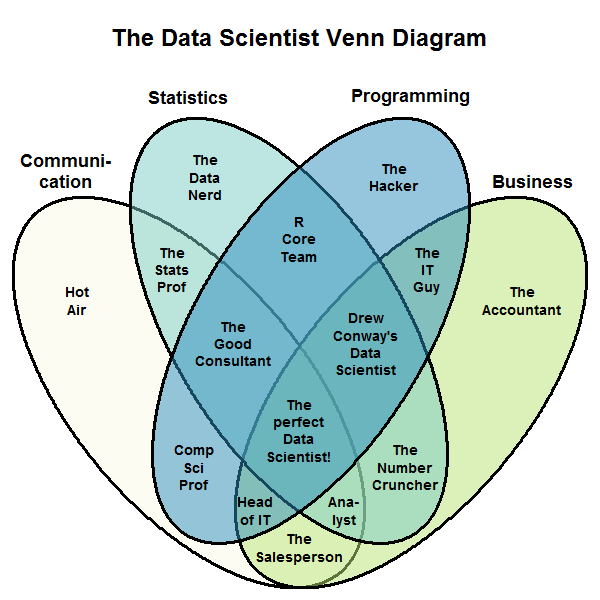
\includegraphics{img/venn1.png}

~

\ldots{} or here is a more popular, simpler version of the same diagram:

~

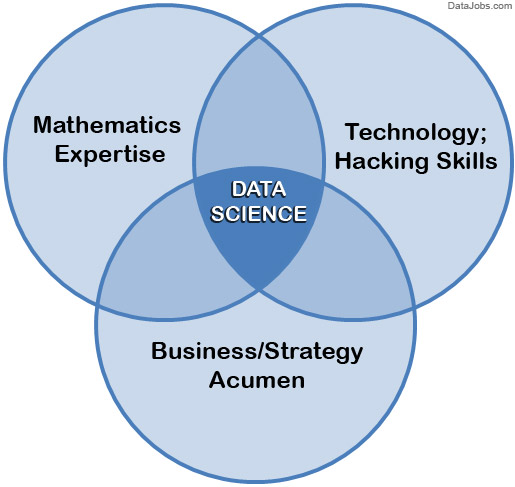
\includegraphics{img/venn5.jpg}

Some argue that data science is simply \href{https://www.statisticsviews.com/article/nate-silver-what-i-need-from-statisticians/}{an extension of statistics}. You will also find attempts to distinguish between categories of data science, or to draw lines around what data science is and what it is not. A classic example is the bizarre delineation corporations draw between a data \emph{scientist} and a data \emph{analyst}:

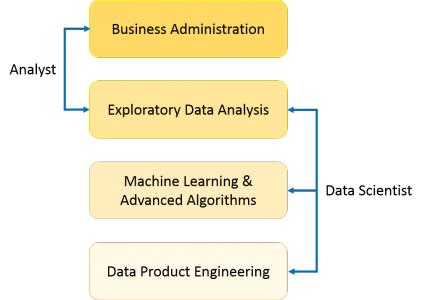
\includegraphics{img/venn2.png}

~
\ldots{} or \ldots{}
~

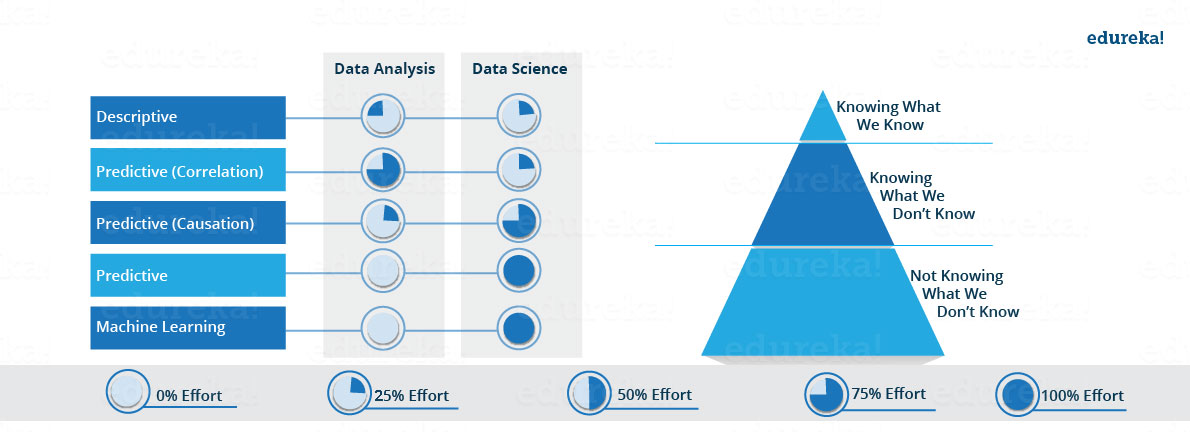
\includegraphics{img/venn3.jpg}

~

\textbf{Our take?} Those definitions are useful, interesting, and to some degree accurate. \emph{But} data science is too new, and too fluid, to be fixed into some static definition. So, to keep our definition accurate, we'll keep it broad:

\textbf{Data science is simply ``doing science with data''.} And for our purposes, the only difference between our definition and the definition of science itself is not in the word ``data'' -- since nowadays all scientists are, to some degree, ``data scientists'' -- but rather in the word ``doing''. Data science is about \emph{doing} stuff with data -- about \emph{making a difference with data.} And that's what this course is going to be about. \emph{DOING}.

But we'll go one step outward. Data science is not just the combination of academic disciplines like stats and business strategy. Good data science also needs to involve (1) \textbf{domain knowledge} (i.e., familiarity with the problem being solved), (2) \textbf{a bias to real-world effects} rather than theoretical frameworks, and (3) \textbf{a desire to work in the real world}. To do so, data scientists generally need to be effective communicators and have an iterative mentality: they try something, evaluate its effects, try something else, and repeat.

Our definition is very broad, we know. We consider the ``analyst'' working in business intelligence to be a data scientist; and so too do we think that a data scientist could be an engineer who is processing large amounts of data to extract basic trends. Again, data scientists are those who \emph{do science with data}. That's a lot of people.

In our experience, the best data scientists aren't simply the best programmers or best statisticians; the best ones are the people who consider themselves to be \emph{something else first.} They are the journalists, artists, epidemiologists, psychologists, historians, environmentalists, sports analysts, and political commentators who \emph{also} know how to work with data. In other words, the best data scientists are the ones already out there, on the ground, already embedded in the system they want to improve, positioned perfectly to get the right data, to ask the right questions, and to actually \emph{do} something with insights from the data. Again, data science is about \emph{DOING}.

To summarize, data science is about applying data to problems. It is impact-driven, transdisciplinary, and suited to well-rounded, multi-dimensional professionals.

\hypertarget{what-is-the-data-life-cycle}{%
\section*{What is the data life cycle?}\label{what-is-the-data-life-cycle}}
\addcontentsline{toc}{section}{What is the data life cycle?}

There is a misperception about data science work that it is largely or even exclusively interpretative: that is, a data scientist looks at a big set of data and builds a fancy statistical model, then a light bulb goes off in her head, she has some insight, and then acts on that insight.

The reality is data science is much more than that. And most of data science is a combination of \emph{(a)} getting data ready for analysis, \emph{(b)} hypothesis testing, and \emph{(c)} figuring out what to do with the results of \emph{a} and \emph{b}. That is, data science in practice is generally not some artesenal genius staring at a table of numbers until ``insight'' magically occurs. Rather, it is a lot of work, a lot of structured theories which can be confirmed or falsified, and a lot of \emph{imagination} applied to the task of implementation.

In other words, data goes through a whole \emph{lifecycle} of which analysis is just a small part.

What is the data lifecycle? Here's how we conceptualize it:

\textbf{0. Observation}\\
\textbf{1. Problem identification \& definition}\\
\textbf{2. Question formation}\\
\textbf{3. Hypothesis generation}\\
\textbf{4. Data collection}\\
\textbf{5. Data processing}

This step is usually the most intensive. Half the battle is wrangling raw data and making it ready for a visualization or a hypothesis test. Note that this step has \emph{nothing to do with statistical tests} -- data science is not the same as statistics!

\textbf{6. Model building / hypothesis testing}

Note that this step is usually where the scientific method stops. In science, once you analyze your test, you interpret your results and loop back to the beginning of the data cycle. But in \emph{applied data science}, there are a few more steps:

\textbf{7. Operationalization:} This means determining how best to incorporate the data insights into operations.

\textbf{8. Communication / dissemination}

\textbf{9. Action:} This means actually implementing the change.

\textbf{10. Observation:} back to the beginning of the cycle.

Again, the above should look a lot like the scientific method. The main differences are (a) ``data processing'', which in reality takes up most of any data scientist's time, (b) the bias towards action, and (c) the iterative / looped nature of the lifecycle.

\hypertarget{data-science-in-the-wild}{%
\section*{Data science `in the wild'}\label{data-science-in-the-wild}}
\addcontentsline{toc}{section}{Data science `in the wild'}

Enough theory. What do data scientists actually do? Again, you can search for an answer online and find complex diagrams like this one:

~

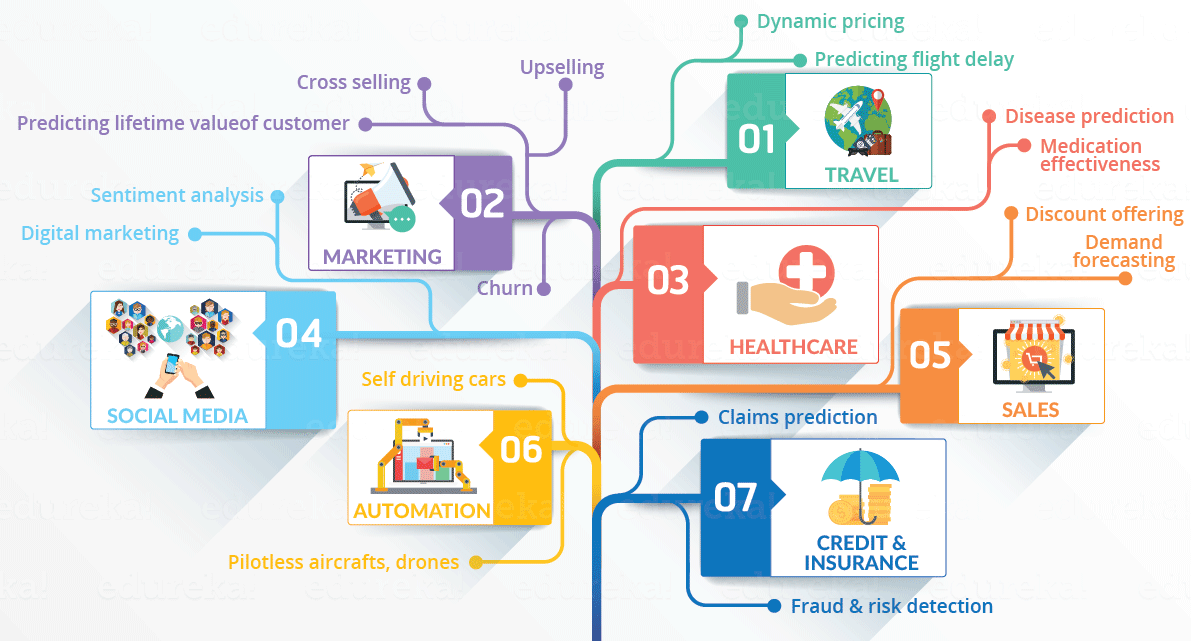
\includegraphics{img/venn4.png}

~

But to capture every problem that data scientists are working on, this diagram would have to be even more convoluted and complex.
Data scientists are working on a \emph{ton} of problems.

The most stereotypical data science problems tend to involve advertising, social media, and corporate profiteering:

\begin{itemize}
\tightlist
\item
  Targeted advertising\\
\item
  Social media feed optimization (getting you to scroll just a little further)
\item
  Facial recognition (automated tagging at Facebook)
\item
  Voice recognition (`Hey, Siri!', `Alexa!')
\item
  Making video games more fun / addictive\\
\item
  Dynamic airline pricing\\
\item
  Search autocomplete\\
\item
  Autocorrect\\
\item
  Virtual assistants
\end{itemize}

These are the kinds of problems that the best-paid data scientists in the world are working to solve. Right now there are thousands of programmers in Mountain View, Cupertino, and elsewhere in the Bay Area (and New York, and London, and Beijing) trying to solve the problem of you not spending enough time on social media.

Maybe you care about these problems, maybe you don't. Maybe they make you indignant or angry. Maybe you find it \emph{problematic} that these things are even considered problems at all. As far as we're concerned, it is deeply unfortunate that our highest-paid data scientists are focusing on problems like these.

But take heart -- there are plenty of other data scientists out there working on \emph{actual} problems that are actually \emph{important}:

\begin{itemize}
\tightlist
\item
  Identifying disease through imagery\\
\item
  Automating identification of credit card fraud\\
\item
  Filtering spam with malware or viruses.\\
\item
  Preventive maintenance at nuclear facilities\\
\item
  Improving chemotherapy dosage\\
\item
  Increasing voter turnout\\
\item
  Improve matchmaking systems (liver transplants, love, etc.)\\
\item
  Measuring deforestation with satellite imagery.\\
\item
  Efficient and equitable vaccine distribution\\
\item
  Identifying tax evaders\\
\item
  Predictive policing\\
\item
  Storm surge forecasting\\
\item
  Identifying and removing child pornography from the internet\\
\item
  Surveilling emergency rooms to predict disease outbreaks\\
\item
  Detecting fake news\\
\item
  Increasing accountability and legitimacy of carbon markets\\
\item
  Quantifying the likelihood of recidivism to prevent over-incarceration
\end{itemize}

The list goes on. The number of worthwhile problems waiting for data scientists is limitless, there are data scientists working on problems like these right now, and the demand for civic-minded data scientists is immense.

All of this matters for a lot of reasons. The first is that data science is not always a good thing; it can be weaponized by corporations and governments in spite of the public interest, and for that we need to be very careful about how we use it and how we teach it.

But the second reason this matters is that data science can be an \emph{equally powerful force for social good}. We can use data science to make progress on the most urgent and injurious social and environmental problems of our time.

However -- and this is the third reason all this matters -- data science can only achieve social good \emph{if} we recruit students to its ranks who are values-driven, civic-minded, and committed to using data science for good.

Fourth, and finally, this matters because the Facebook data scientists are using the exact same principles and basic tools as the non-profit data scientists. At their core, the foundational skillsets are the same.

And that's what this book is all about.

\hypertarget{the-reproducibility-crisis}{%
\chapter{The reproducibility crisis}\label{the-reproducibility-crisis}}

\hypertarget{the-crisis}{%
\section*{The crisis}\label{the-crisis}}
\addcontentsline{toc}{section}{The crisis}

There is a crisis in the sciences: the reproducibility crisis. It is also known as the replication crisis. This refers to the fact that many scientific studies have been impossible to reproduce, calling into question the validity of those studies' findings.

This crisis began in the mid-2000's, when psychologists realized they could not reproduce most of their colleagues' results. They tried to repeat the experiments, following the methods step-by-step, but failed to get the same results. This was enormously unsettling for psychologists, and it cast major doubts upon the validity of psychological theory.

The realization that much of published research is not actually reproducible soon spread to medical research\ldots{}

~

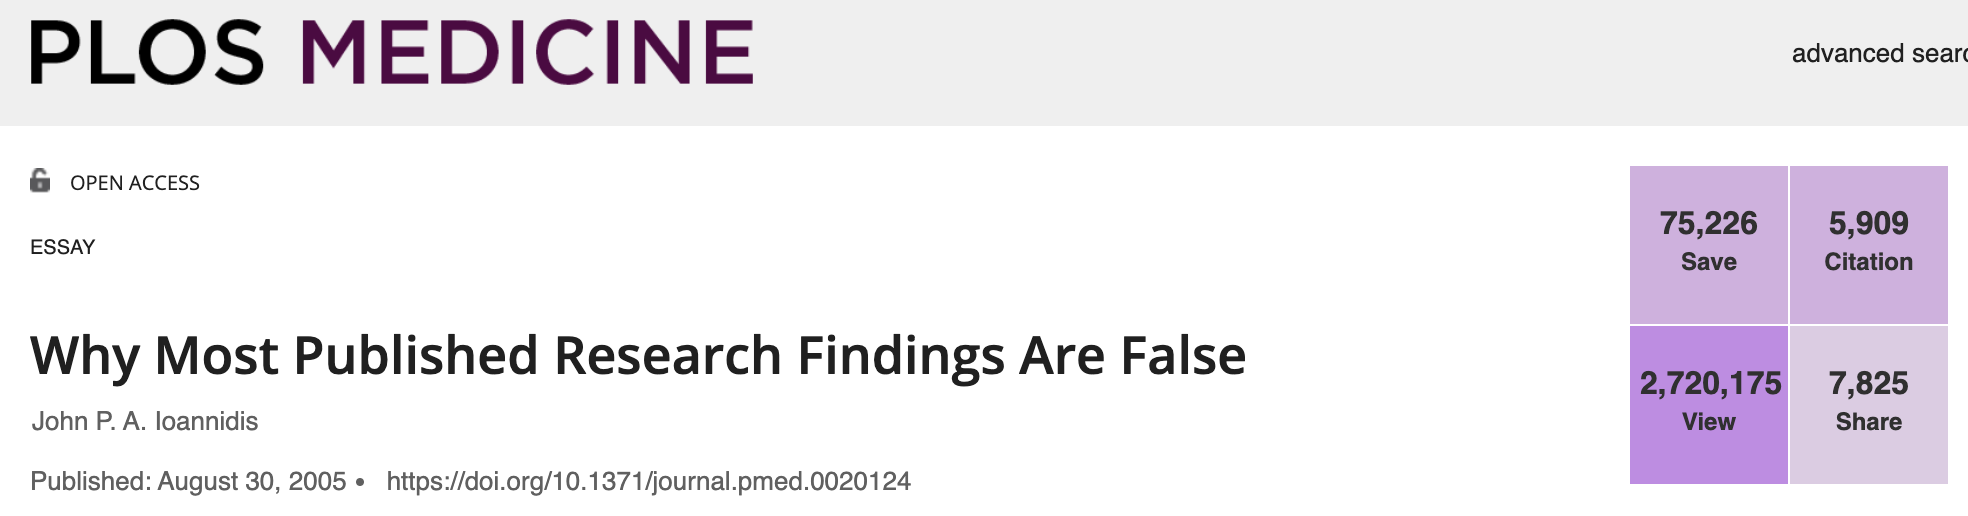
\includegraphics{img/reproducibility-psych.png}

~

\ldots then it sprung up in marketing\ldots{}

~

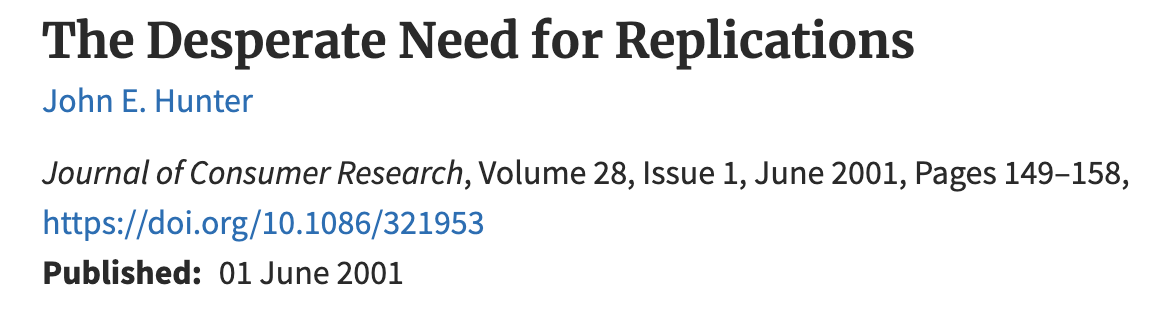
\includegraphics{img/reproducibility-marketing.png}
~

\ldots and economics\ldots{}

~

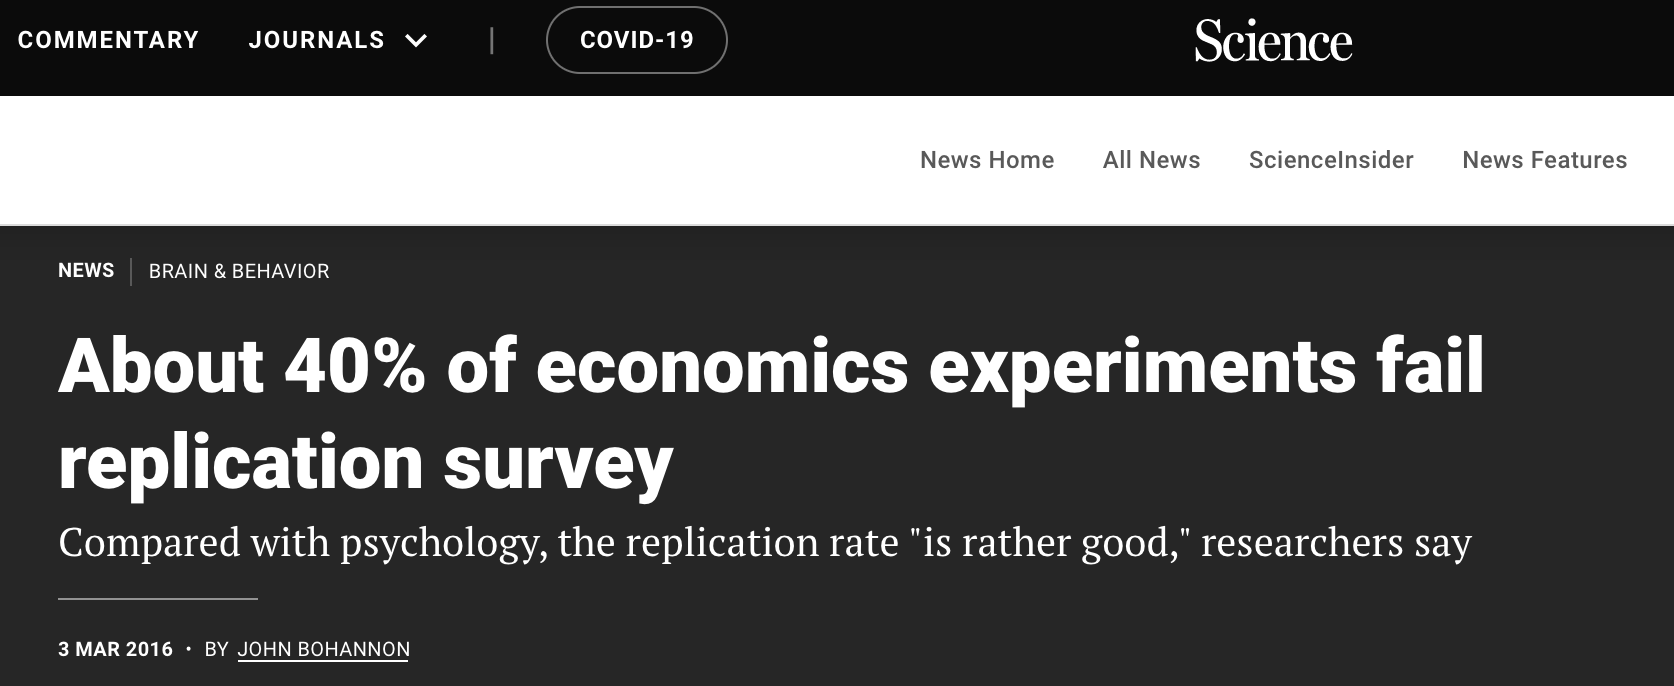
\includegraphics{img/reproducibility-econ.png}
~

\ldots and the sports sciences\ldots{}

~

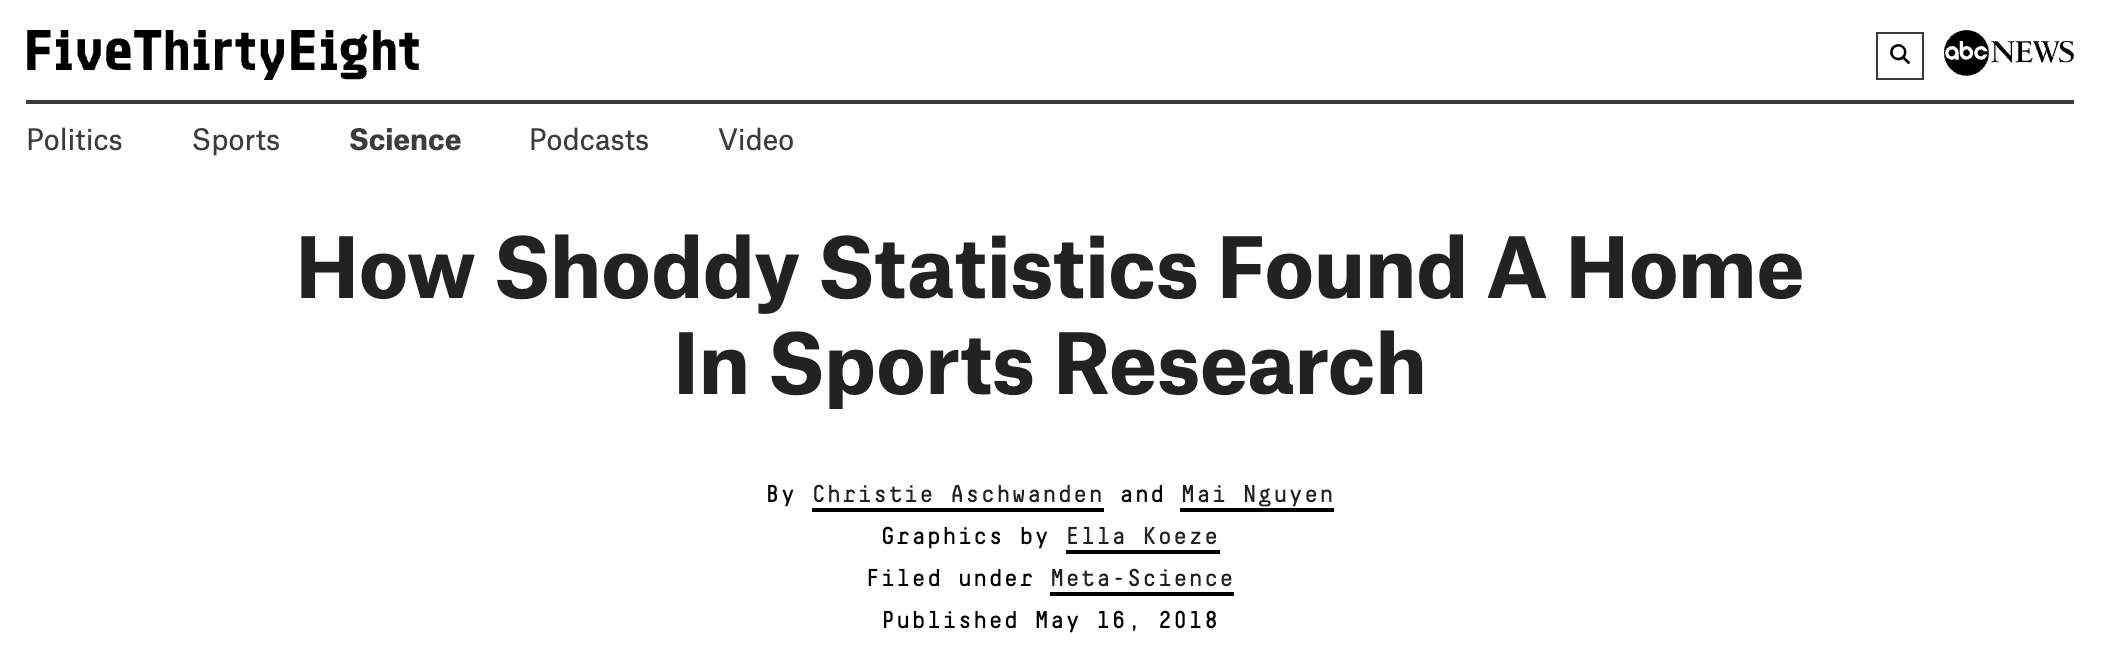
\includegraphics{img/reproducibility-sports.png}
~

\ldots and the life sciences too:

~

For a complete history of the crisis, check out this article from \href{https://en.wikipedia.org/wiki/Replication_crisis}{Wikipedia}.

\textbf{Why is this happening?} There are many reasons. Many studies, particularly those in psychology and the social sciences, involve small cohorts of participants. When sample sizes are low, results may not be representative of underlying truths.

On rare occasions it is intentional and fraudulent: scientists face pressure to publish interesting results, so much so that they might fabricate or filter their data to make their results significant.

But the most common causes of reproducibility failure are, by far, (1) \textbf{poorly documented steps in data processing} -- if you don't know how exactly the authors of a paper formatted their raw data to prepare them for analysis, you simply can't reproduce the analysis -- and (2) simple, \textbf{honest mistakes}, such as typos in spreadsheets.

Consider this summary of the reproducibility crisis from \emph{The Economist}. A scary percentage of genomics studies have simple spreadhseet errors:

~

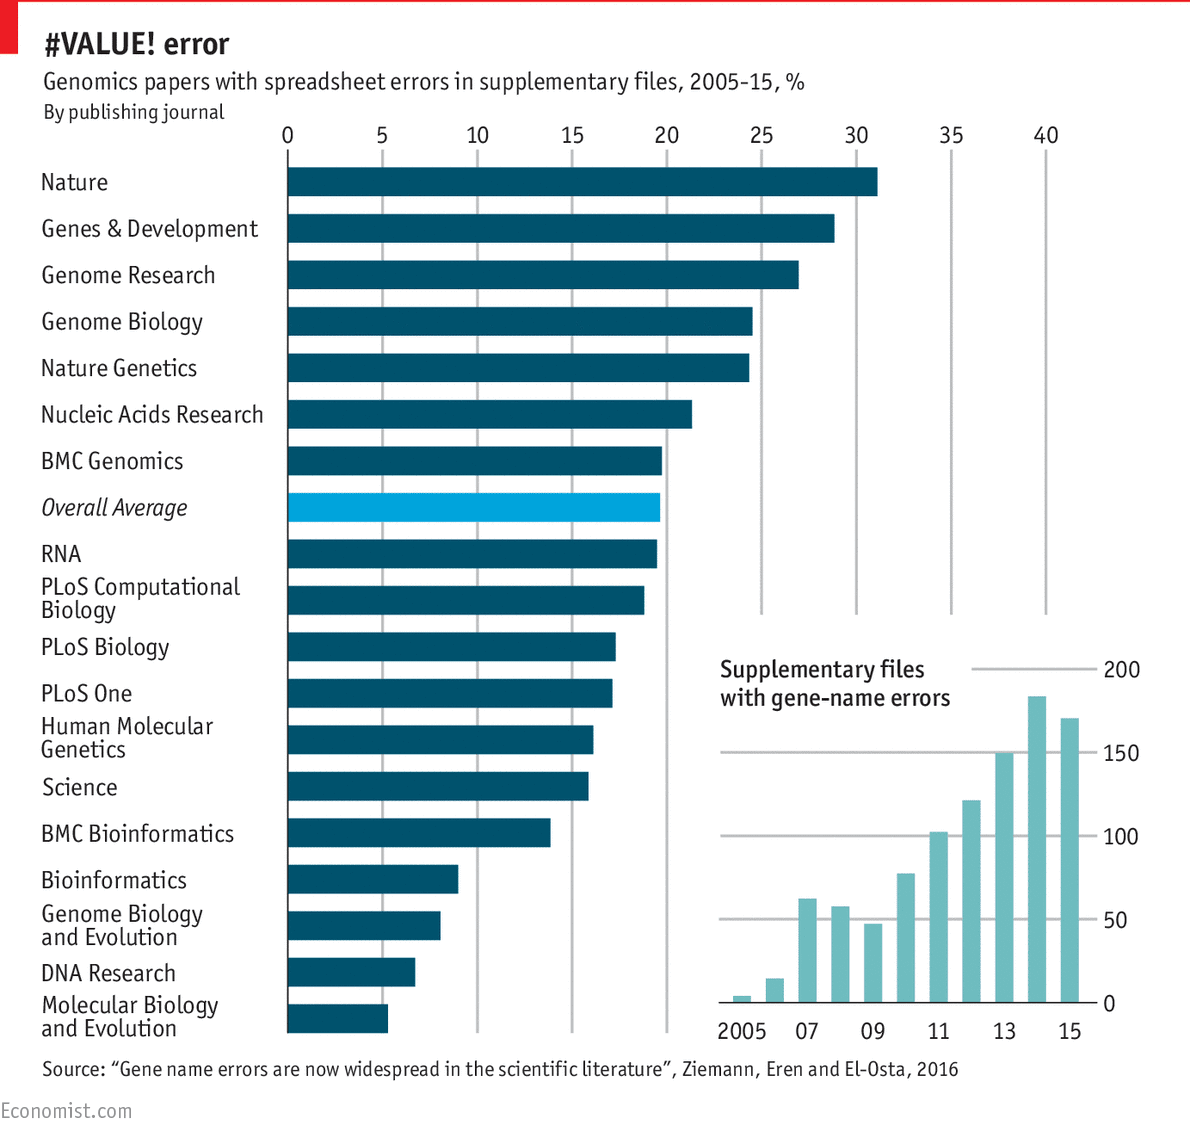
\includegraphics{img/reproducibility-economist.png}
~

\textbf{This is a big deal:} if a significant part of science is \emph{wrong}, then what do we know? How can we be sure what we know is right? How can we build off of previous research? How can we distinguish valid science from the rest? If science can't be trusted, what value does it have for society? What kind of \emph{damage} is it doing to society?

\textbf{This crisis is ongoing}, and it is impacting our handling of the COVID-19 pandemic. On October 5, 2020, the world learned that 16,000 COVID-19 cases disappeared from the UK's public health database due to a simple glitch in \emph{Microsoft Excel}.

~

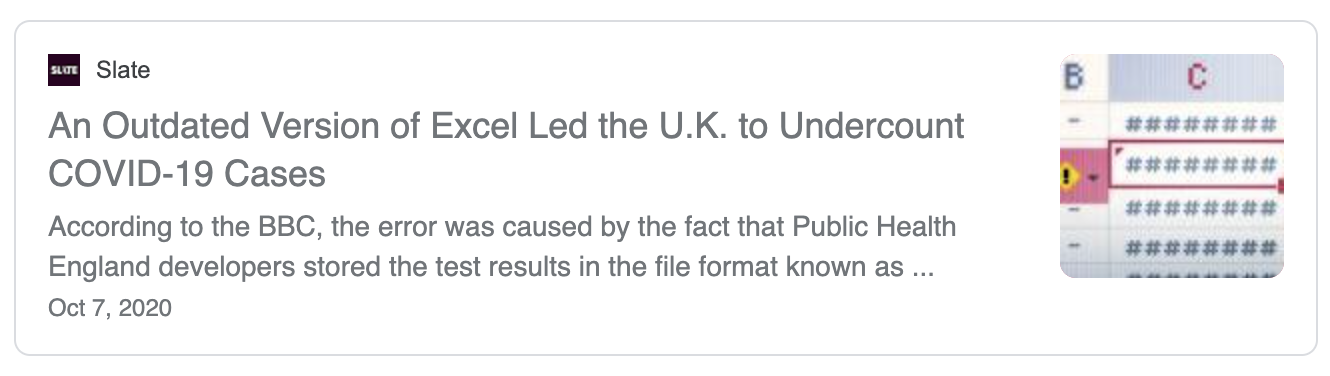
\includegraphics{img/reproducibility-covid-1.png}

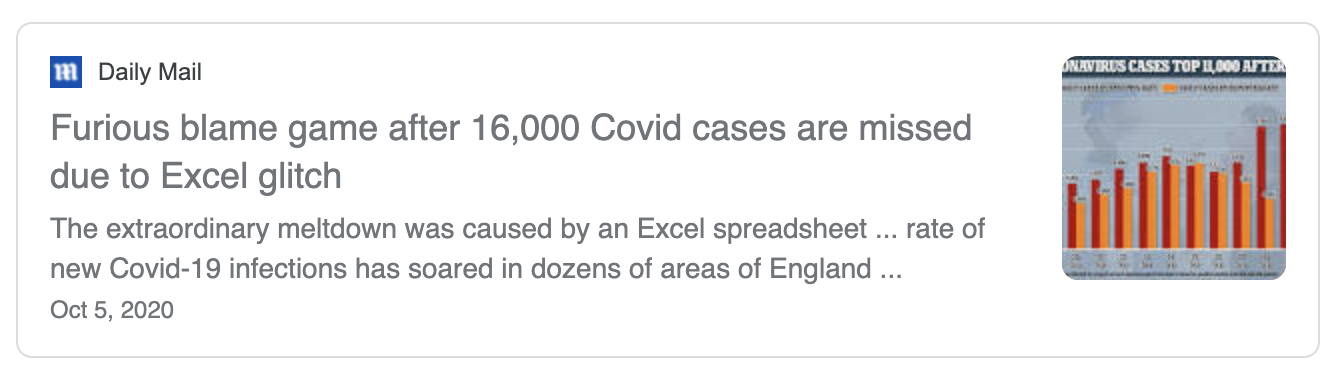
\includegraphics{img/reproducibility-covid-2.png}
~

That event demonstrated that the reproducibility crisis is not just an academic concern. It can have serious and potentially deadly consequences for the public.

But there are \textbf{silly examples} of the replication crisis, too. Perhaps our favorite is this: in August 2021, when we Google'd ``reproducibility crisis'', one of the top search results is this video from \emph{Science}, the world's most prestigious scientific journal:


\includegraphics{img/reproducibility-1.png}

~

But when we click on this link, here's what we see:

~

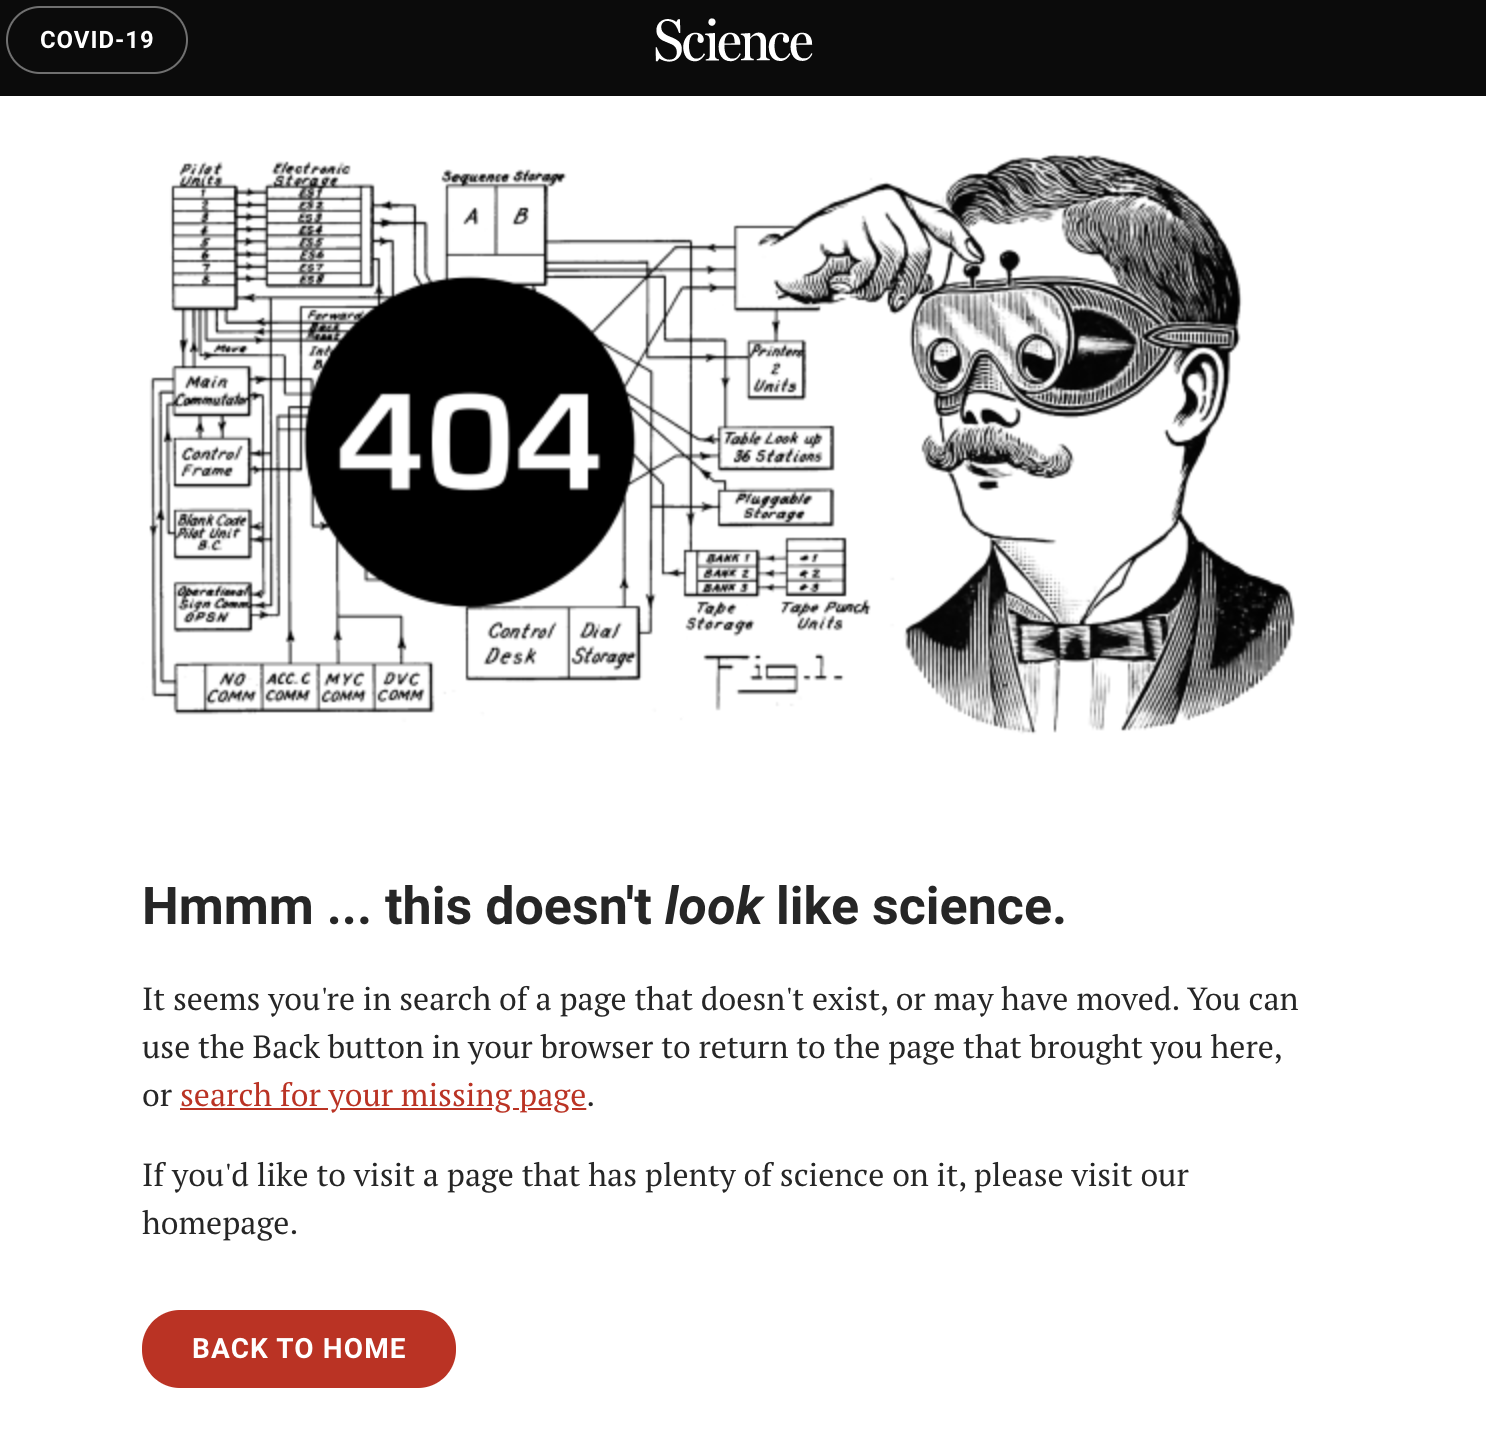
\includegraphics{img/reproducibility-2.png}

\hypertarget{the-reproducibility-movement}{%
\section*{The `reproducibility' movement}\label{the-reproducibility-movement}}
\addcontentsline{toc}{section}{The `reproducibility' movement}

Because of this crisis, there has emerged a much needed move to make all science ``reproducible''. This means making sure that someone else can copy what you did, and get the same results. This is important for identifying scientific fraud, of course, but also for helping us to overcome human bias, mistakes, wishful thinking, etc. Reproducibility is not just a ``nice-to-have''; in modern science (and data science), it's a ``must''.

\textbf{Good data science must be reproducible.} The idea is that work done by scientist A is ``reproducible'' by scientist B. In other words, if the findings of the research are of any generalizable value, then the results of two scientists working on the same problem should be identical (or very high in agreement). In practice, this means using data and code in a structured, well-documented, accessible, clear way, and ensuring that others can do the same.

Reproducible research also means using tools that others can easily use, and methods that others can easily copy. Programming languages like \texttt{R} and \texttt{Python} are ideal for this.

Reproducible research matters for lots of reasons:

\begin{enumerate}
\def\labelenumi{\arabic{enumi}.}
\tightlist
\item
  Because making your work reproducible means that \emph{you} will have less problems returning to that work at a later time.\\
\item
  Because making your work reproducible means that \emph{others} can collaborate with you, help you, error-check you, and build on your work.\\
\item
  Because making your work reproducible means you are fighting the plague of irreproducible results which have characterized the replication crisis.
\end{enumerate}

Making your work reproducible is going to be a bit more work, but it's not optional. And there are tools and best practices in place to make it as painless as possible. Basically, reproducible research involves the following:

\begin{itemize}
\item
  Using code to format and manage your data instead of spreadsheet software such as \emph{Excel} or \emph{GoogleSheets}, since those products will not keep a step-by-step record of each thing that you do. When you code, each command line is both an action you take to process your data \emph{and} a record of what that action is.
\item
  Coding with free, open-source tools, such as \texttt{R}.
\item
  For any specific niche task in your analysis, such as processing a batch of images, using other open source tools (e.g., \texttt{ImageJ}) that can be used free-of-charge by anyone with an internet connection anywhere.
\item
  Documenting \emph{everything} you do with the data, by commenting your code thoroughly and by creating ``Wiki'' pages for your projects.
\item
  Making your code open source and freely available online.
\item
  Making your data open source (while protecting privacy and confidentiality of participants).
\item
  Providing tools, such as \texttt{Shiny} in \texttt{R}, that allow others to explore your data themselves, rather than trusting your own narratives about the data.
\item
  Using tools for generating reports, such as \texttt{Rmarkdown}, that remove the `middle-man' and avoid potential typo's and fabrications.
\item
  Collaborating openly with others.
\end{itemize}

You will be learning how to do all of these things in this course. We are going to focus on \emph{reproducible research}, \emph{literate programming}, \emph{documentation}, and other components of data science (and research in general) which ensure that (a) our methods and findings can be easily sanity-tested by others, and (b) we set ourselves and our projects' up for future collaborations, hand-offs, and expansion.

\hypertarget{why-r}{%
\section*{\texorpdfstring{Why \texttt{R}?}{Why R?}}\label{why-r}}
\addcontentsline{toc}{section}{Why \texttt{R}?}

This course is largely about learning to \emph{do}, and will largely use \texttt{R}. \texttt{R} is not the only tool in the data scientists' toolbox (there are many), but it's a good one, is extremely popular, there is almost nothing you cannot do with it, it can be applied to many fields, and -- most importantly -- it is a free, open-source tool with an active open-source coding community. The millions of \texttt{R} users worldwide emulate the spirit of reproducible research we are trying to advocate for here.

\hypertarget{a-final-thought}{%
\subsection*{A final thought}\label{a-final-thought}}
\addcontentsline{toc}{subsection}{A final thought}

A research article about \emph{results} is advertising, not scholarship.

Scholarship is an article with transparent, reproducible methods.

\hypertarget{data-ethics}{%
\chapter{Data ethics}\label{data-ethics}}

\hypertarget{a-few-principles}{%
\section*{A few principles}\label{a-few-principles}}
\addcontentsline{toc}{section}{A few principles}

This orientation to the principles of data ethics is not going to be adequate or sufficient. We just need to provide enough context for you (1) to appreciate the limitless complexity and uncertainty of many ethical issues in data science, and (2) to start exploring the complex ethical scenarios below on your own or in dialogue with others.

In most frameworks for data ethics, three foundational principles are used to help us think about whether certain research actions are ethical. Those three principles are:

\textbf{1. Respect} for persons and their autonomy: participation must be based upon informed consent, and privacy must be honored at all times. Immature or incapacitated persons must be protected as they mature or heal.

\textbf{2. Beneficence:} in our work with data, potential risks are minimized while potential benefits are maximized.

\textbf{3. Justice:} Benefits and risks are distributed equally across groups of people. A classic way of asking whether something is `just' is asking using John Rawls' concept of the \textbf{`veil of ignorance'}: pretend you have no information at all about your circumstances or your place in the social order: You don't know your place of birth, year of birth, sex, skin color, language, religion, immigration status, health conditions, or anything else. In other words, you have no information whatsoever that might introduce bias into the way you think about the world. Free of circumstantial bias, what arrangements would you choose to put in place to maximize fairness and fortune for all, and to minimize the chances that you would get screwed by the system?

These principles can guide us as we navigate ethically ambiguous scenarios. When we ask whether something is ethical, we are asking whether all of these principles are upheld. We could also be asking whether the violation of one of these principles might be justified by upholding another in an impactful way.

The question, `Is something ethical?' is usually not easy to answer, particularly when it comes to the use of data in tackling social problems. It is important to note that reasonable people regularly disagree on these ideas; that is why we have committees and drawn-out processes for obtaining permission to use data in research and commerce.

\textbf{So why do these principles matter?} Because without them, we would not be able to have conversations about the ethics of difficult situations. We need articulated principles that we can point to and debate together. Principles like these allow you to have an account for why you feel the way you do about a certain issue. Without that account, we can't learn from each other's perspectives.

Note also that these principles were designed with \textbf{individual human subjects} in mind. It is an open question of active debate how exactly these principles can be applied to \textbf{communities of individuals} all at once -- what exactly does it mean for a group to consent to something? Does every single individual need to consent? The majority? -- or how they translate to our treatment of \textbf{non-human communities}: animals, plants, and places.

Let's stop there and explore some concrete scenarios. For a better orientation to ethical precepts underlying issues of data ethics, \href{https://www.scu.edu/media/ethics-center/technology-ethics/IntroToDataEthics.pdf}{this chapter by Shannon Vallor} is the best open-source resource that we have been able to find. Many of the case studies and scenarios presented below are adapted from that chapter.

\hypertarget{warm-up-scenarios}{%
\section*{Warm up scenarios}\label{warm-up-scenarios}}
\addcontentsline{toc}{section}{Warm up scenarios}

Practice applying the above principles to these scenario questions. For each scenario, describe your \textbf{opinion vector} (the \emph{direction} of your opinion -- yes or no -- and the \emph{strength} of your opinion).

\textbf{Location tracking}\\
Is it ethical for Google to track and store your location information in order to monitor traffic and operating hours of local businesses? Such traffic information is known to help direct emergency service vehicles along the safest and fastest route.

\textbf{Targeted advertising}\\
Is it ethical for internet search engines to tailor advertisements according to your search history?

\textbf{Dynamic pricing}\\
Is it ethical for airfare search engines to adjust ticket prices according to your recent search history?

\textbf{Social media scrolling}\\
Is it ethical for Instagram to count how many milliseconds you spend on each post, then use that info to develop a strategy for getting you to spend more time on its app?

\textbf{Controversial content}\\
You are a data scientist at Facebook. Based on your analyses of user data, you have discovered that when you show readers sensational or hyperbolic content, such as someone ranting that a new vaccine is an attempt at government-subsidized mind control, the readers stay on Facebook longer and scroll through more contet. Since that translates to profits, is it OK for your team to increase the amount of sensational content in users' feeds?

\hypertarget{case-studies}{%
\section*{Case studies}\label{case-studies}}
\addcontentsline{toc}{section}{Case studies}

Use these case studies to reflect upon and discuss the ambiguity, complexity, and dangers of data ethics issues.

\hypertarget{the-facebook-social-contagion-study}{%
\subsection*{The Facebook `Social Contagion' Study}\label{the-facebook-social-contagion-study}}
\addcontentsline{toc}{subsection}{The Facebook `Social Contagion' Study}

In 2014, data scientists from Facebook published an \href{https://www.pnas.org/content/111/24/8788}{article} in a prestigious academic journal. In this article, they demonstrated that the emotions and moods of users could be manipulated by toggling the amount of positive or negative content in their feeds. They found that these emotional effects would then be passed to other users in the social network; in other words, emotions and moods could be seeded and were `contagious'. To carry out this research, they manipulated the Facebook feeds of 689,000 users.

~\\

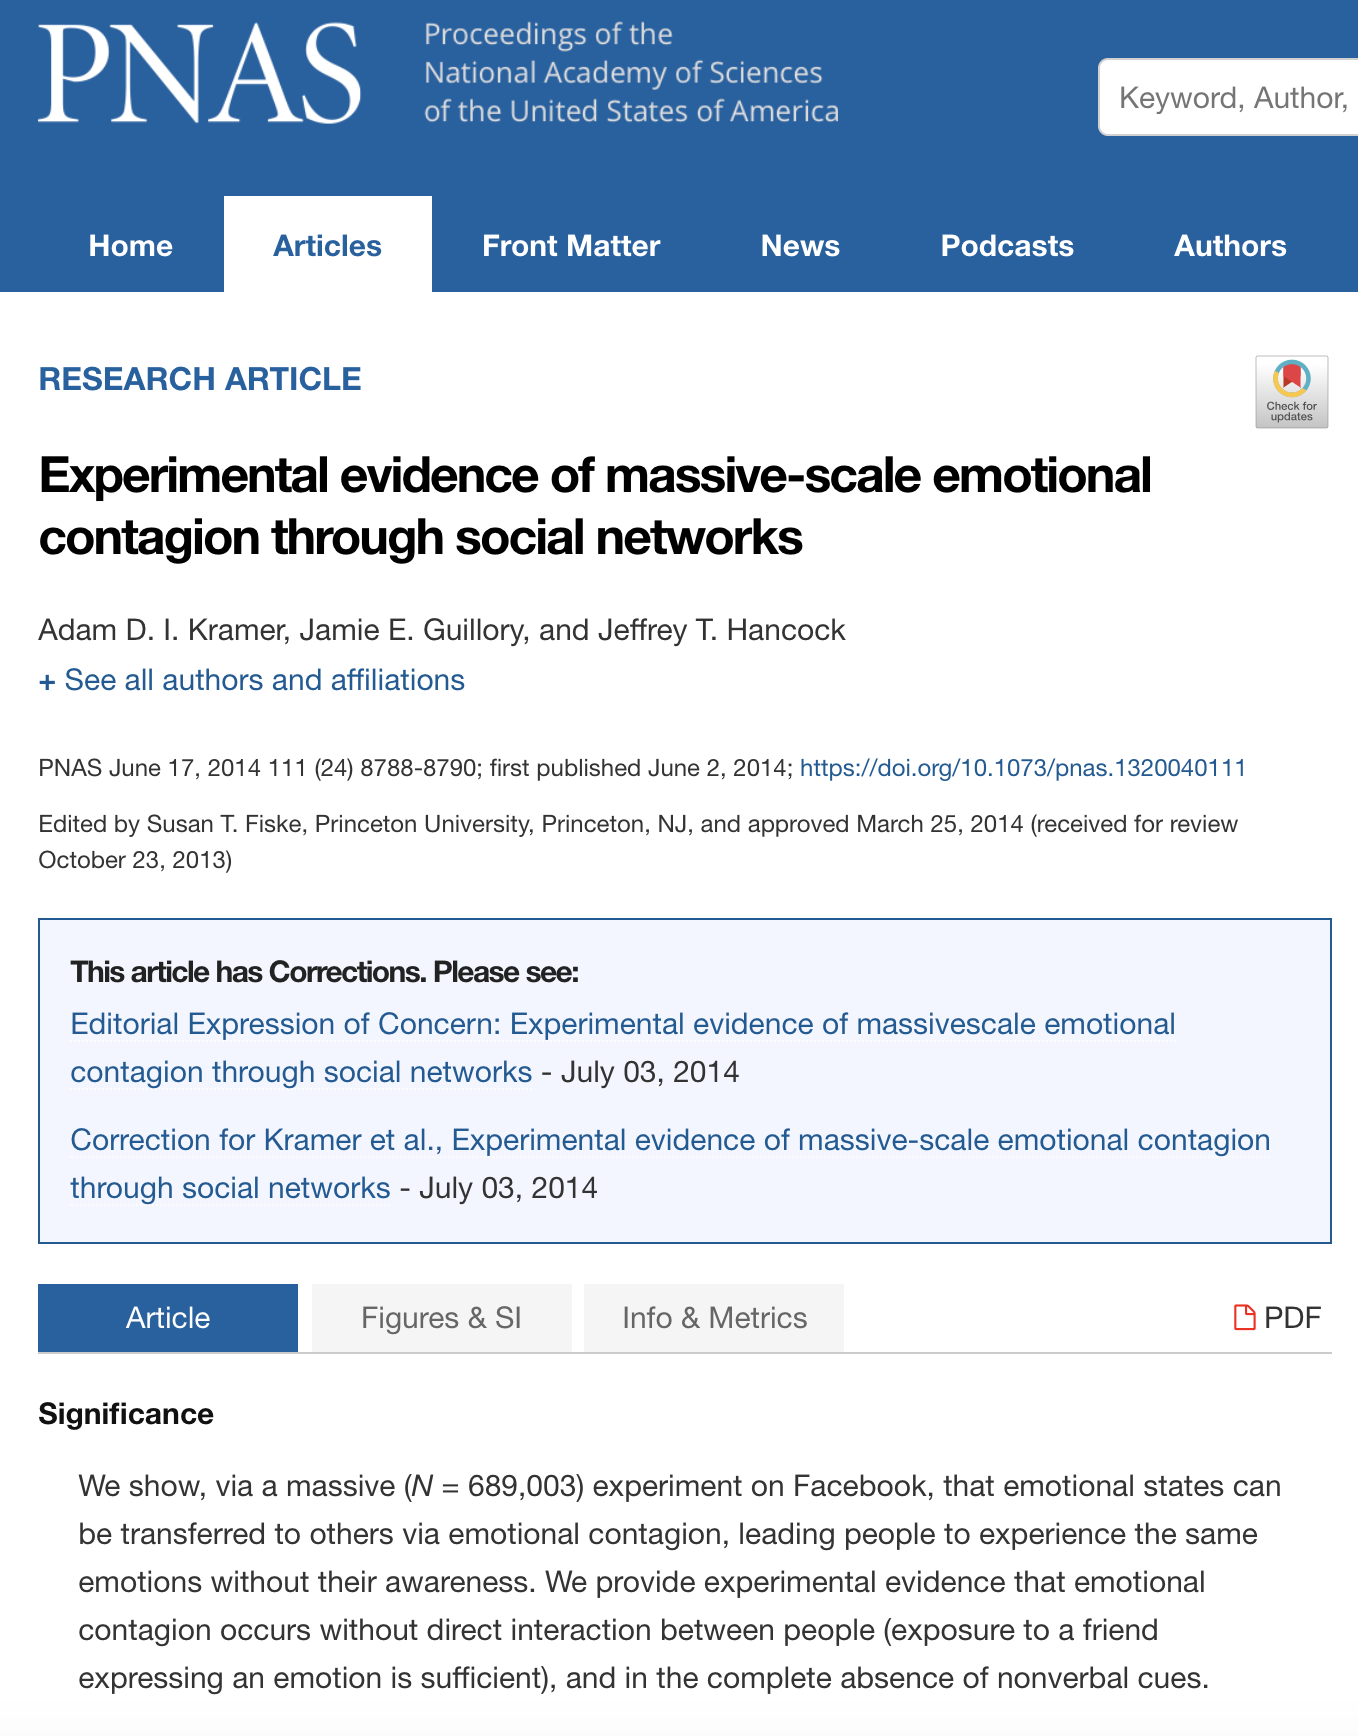
\includegraphics[width=0.7\textwidth,height=\textheight]{img/ethics-fb.png}

~

Facebook did not receive specific consent for this study from its users. Instead, the company argued that the purpose of the study was consistent with the user agreement already in place: to give Facebook knowledge it needs to provide users with a positive experience on the platform.

\textbf{Discuss:}

\begin{enumerate}
\def\labelenumi{\arabic{enumi}.}
\item
  In what ways, specifically, did Facebook violate basic principles of data ethics with this study? Enumerate each violation individually.
\item
  Can a convincing argument be made that justifies this study? What are the strongest arguments in its favor?
\item
  What are some things that Facebook could have done differently to handle this situation more ethically?
\item
  Who exactly should be held morally accountable for any harms caused by this study? The data scientists employed to analyze and publish the data? Mark Zuckerberg? All Facebook employees? Facebook stock holders? Are Facebook users accountable at all?
\end{enumerate}

\hypertarget{machine-bias-beauty-contests-recidivism}{%
\subsection*{Machine bias: Beauty contests \& recidivism}\label{machine-bias-beauty-contests-recidivism}}
\addcontentsline{toc}{subsection}{Machine bias: Beauty contests \& recidivism}

Machine learning (ML) algorithms are developed by `training' models on known datasets. The models are then used to predict values in other datasets. For example, if you label cars in a batch of photos then use them to train a ML model on that labeled dataset, you can then use that model to identify cars in thousands of other photos.

Sounds neat, but this means that ML models are only as good as the data they are trained upon, and often those training datasets are created by human labelers who carry unkown or unspoken biases. A classic example is the \href{https://www.theguardian.com/technology/2016/sep/08/artificial-intelligence-beauty-contest-doesnt-like-black-people}{Beauty.AI} beauty contest that occurred in 2016. A ML algorithm was trained on a large set of human-labeled photos of women, then women around the world were invited to submit selfies in a global beauty contest. A key advertising hook for the contest was that the `robot jury' -- the ML algorithm -- would be fully impartial and fair. But the results revealed that the ML model was racist: 75\% of the 6,000 contestants were white, but 98\% of the 44 winners were white. How did this happen? The people who labeled the training set of photos carried implicit bias.

~\\

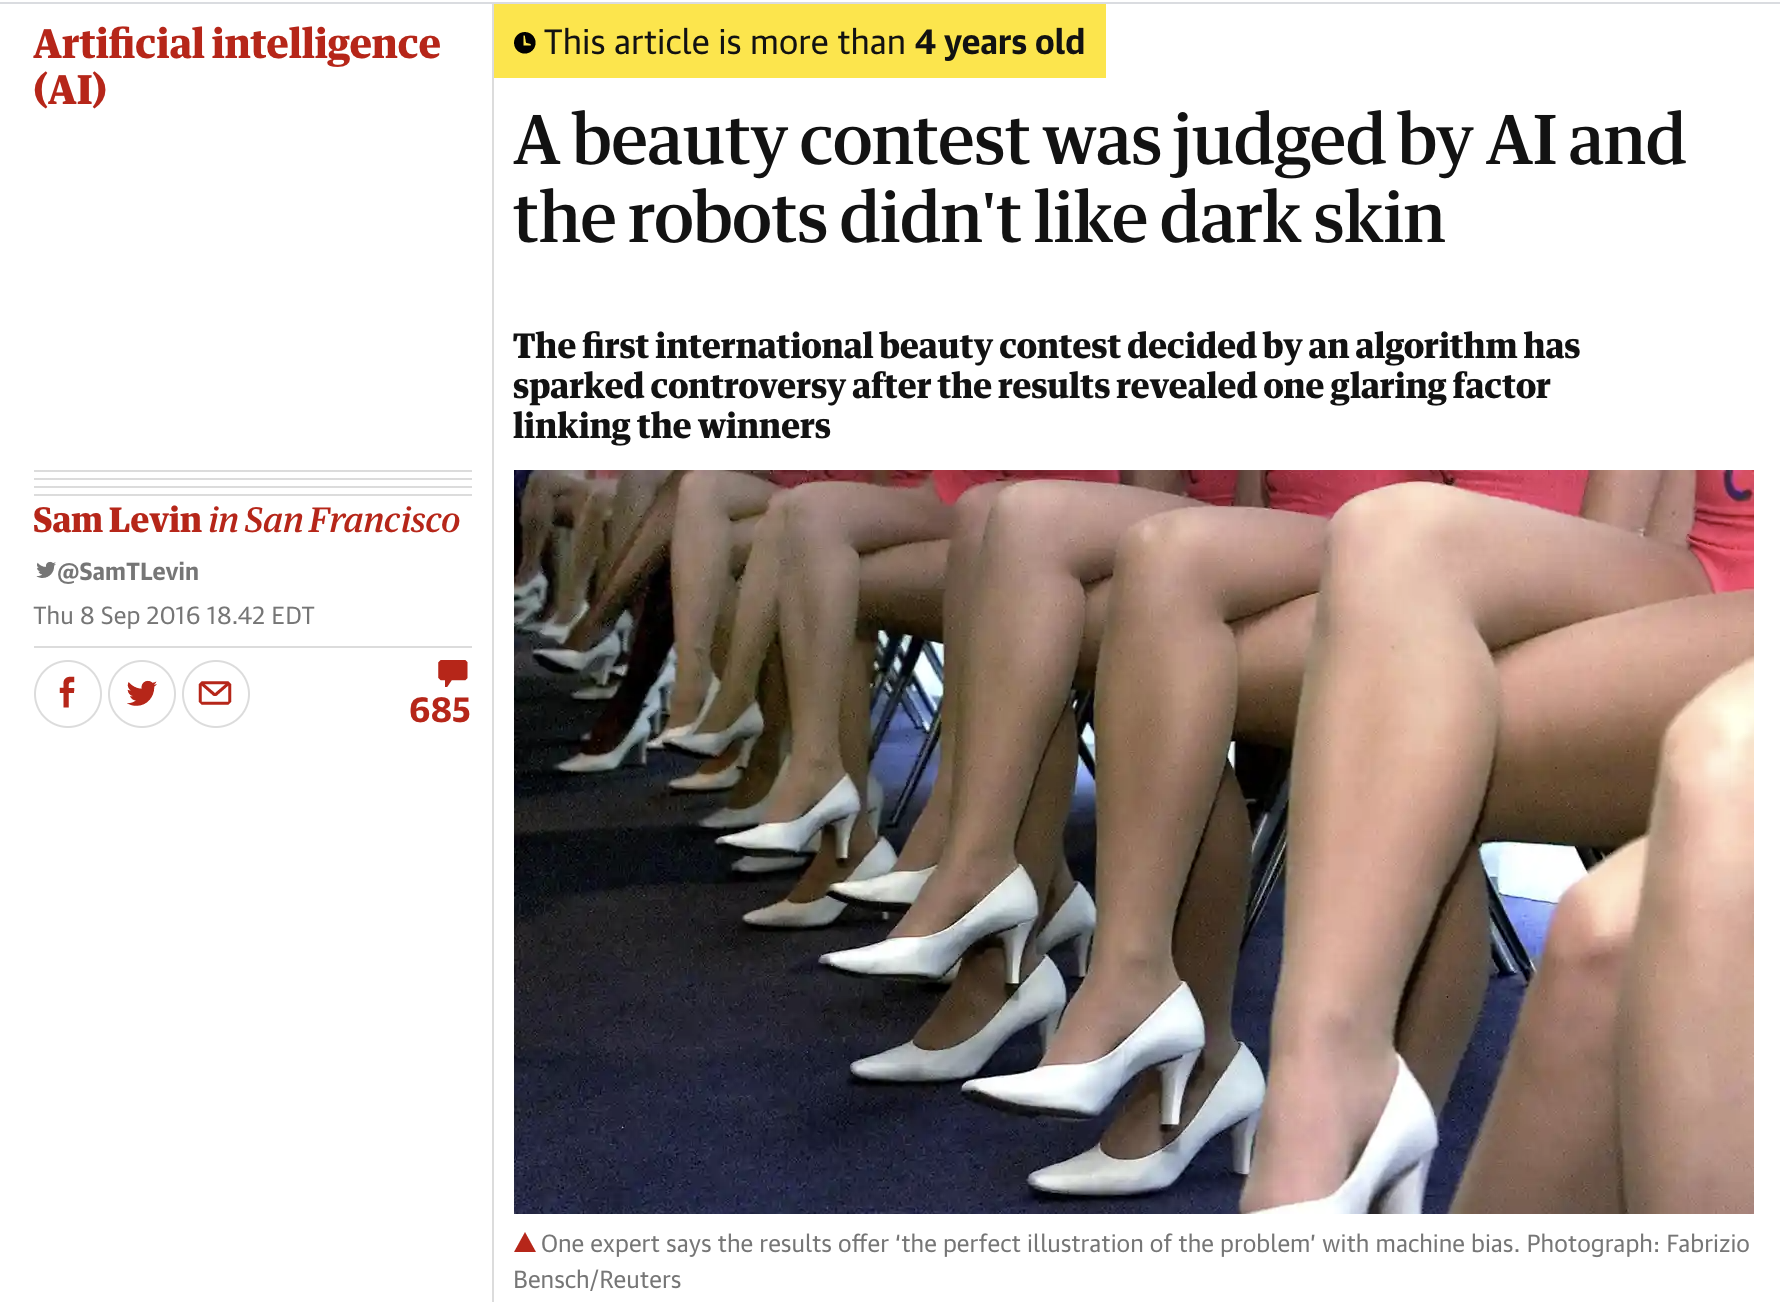
\includegraphics[width=0.7\textwidth,height=\textheight]{img/ethics-machine_bias.png}

~

Debacles like this can have much more serious consequences. \href{https://www.propublica.org/article/machine-bias-risk-assessments-in-criminal-sentencing}{Court systems use ML models} to estimate the risks that a convicted criminal will commit more crimes once they are released from prison. But retrospective studies have shown that these models consistently and incorrectly label black prisoners as more dangerous and more likely to return to prison at a later date. Most of the risk assessments being used today have not received adequate validation, even though they are spitting out predictions that can destroy lives, families, and communities.

~\\

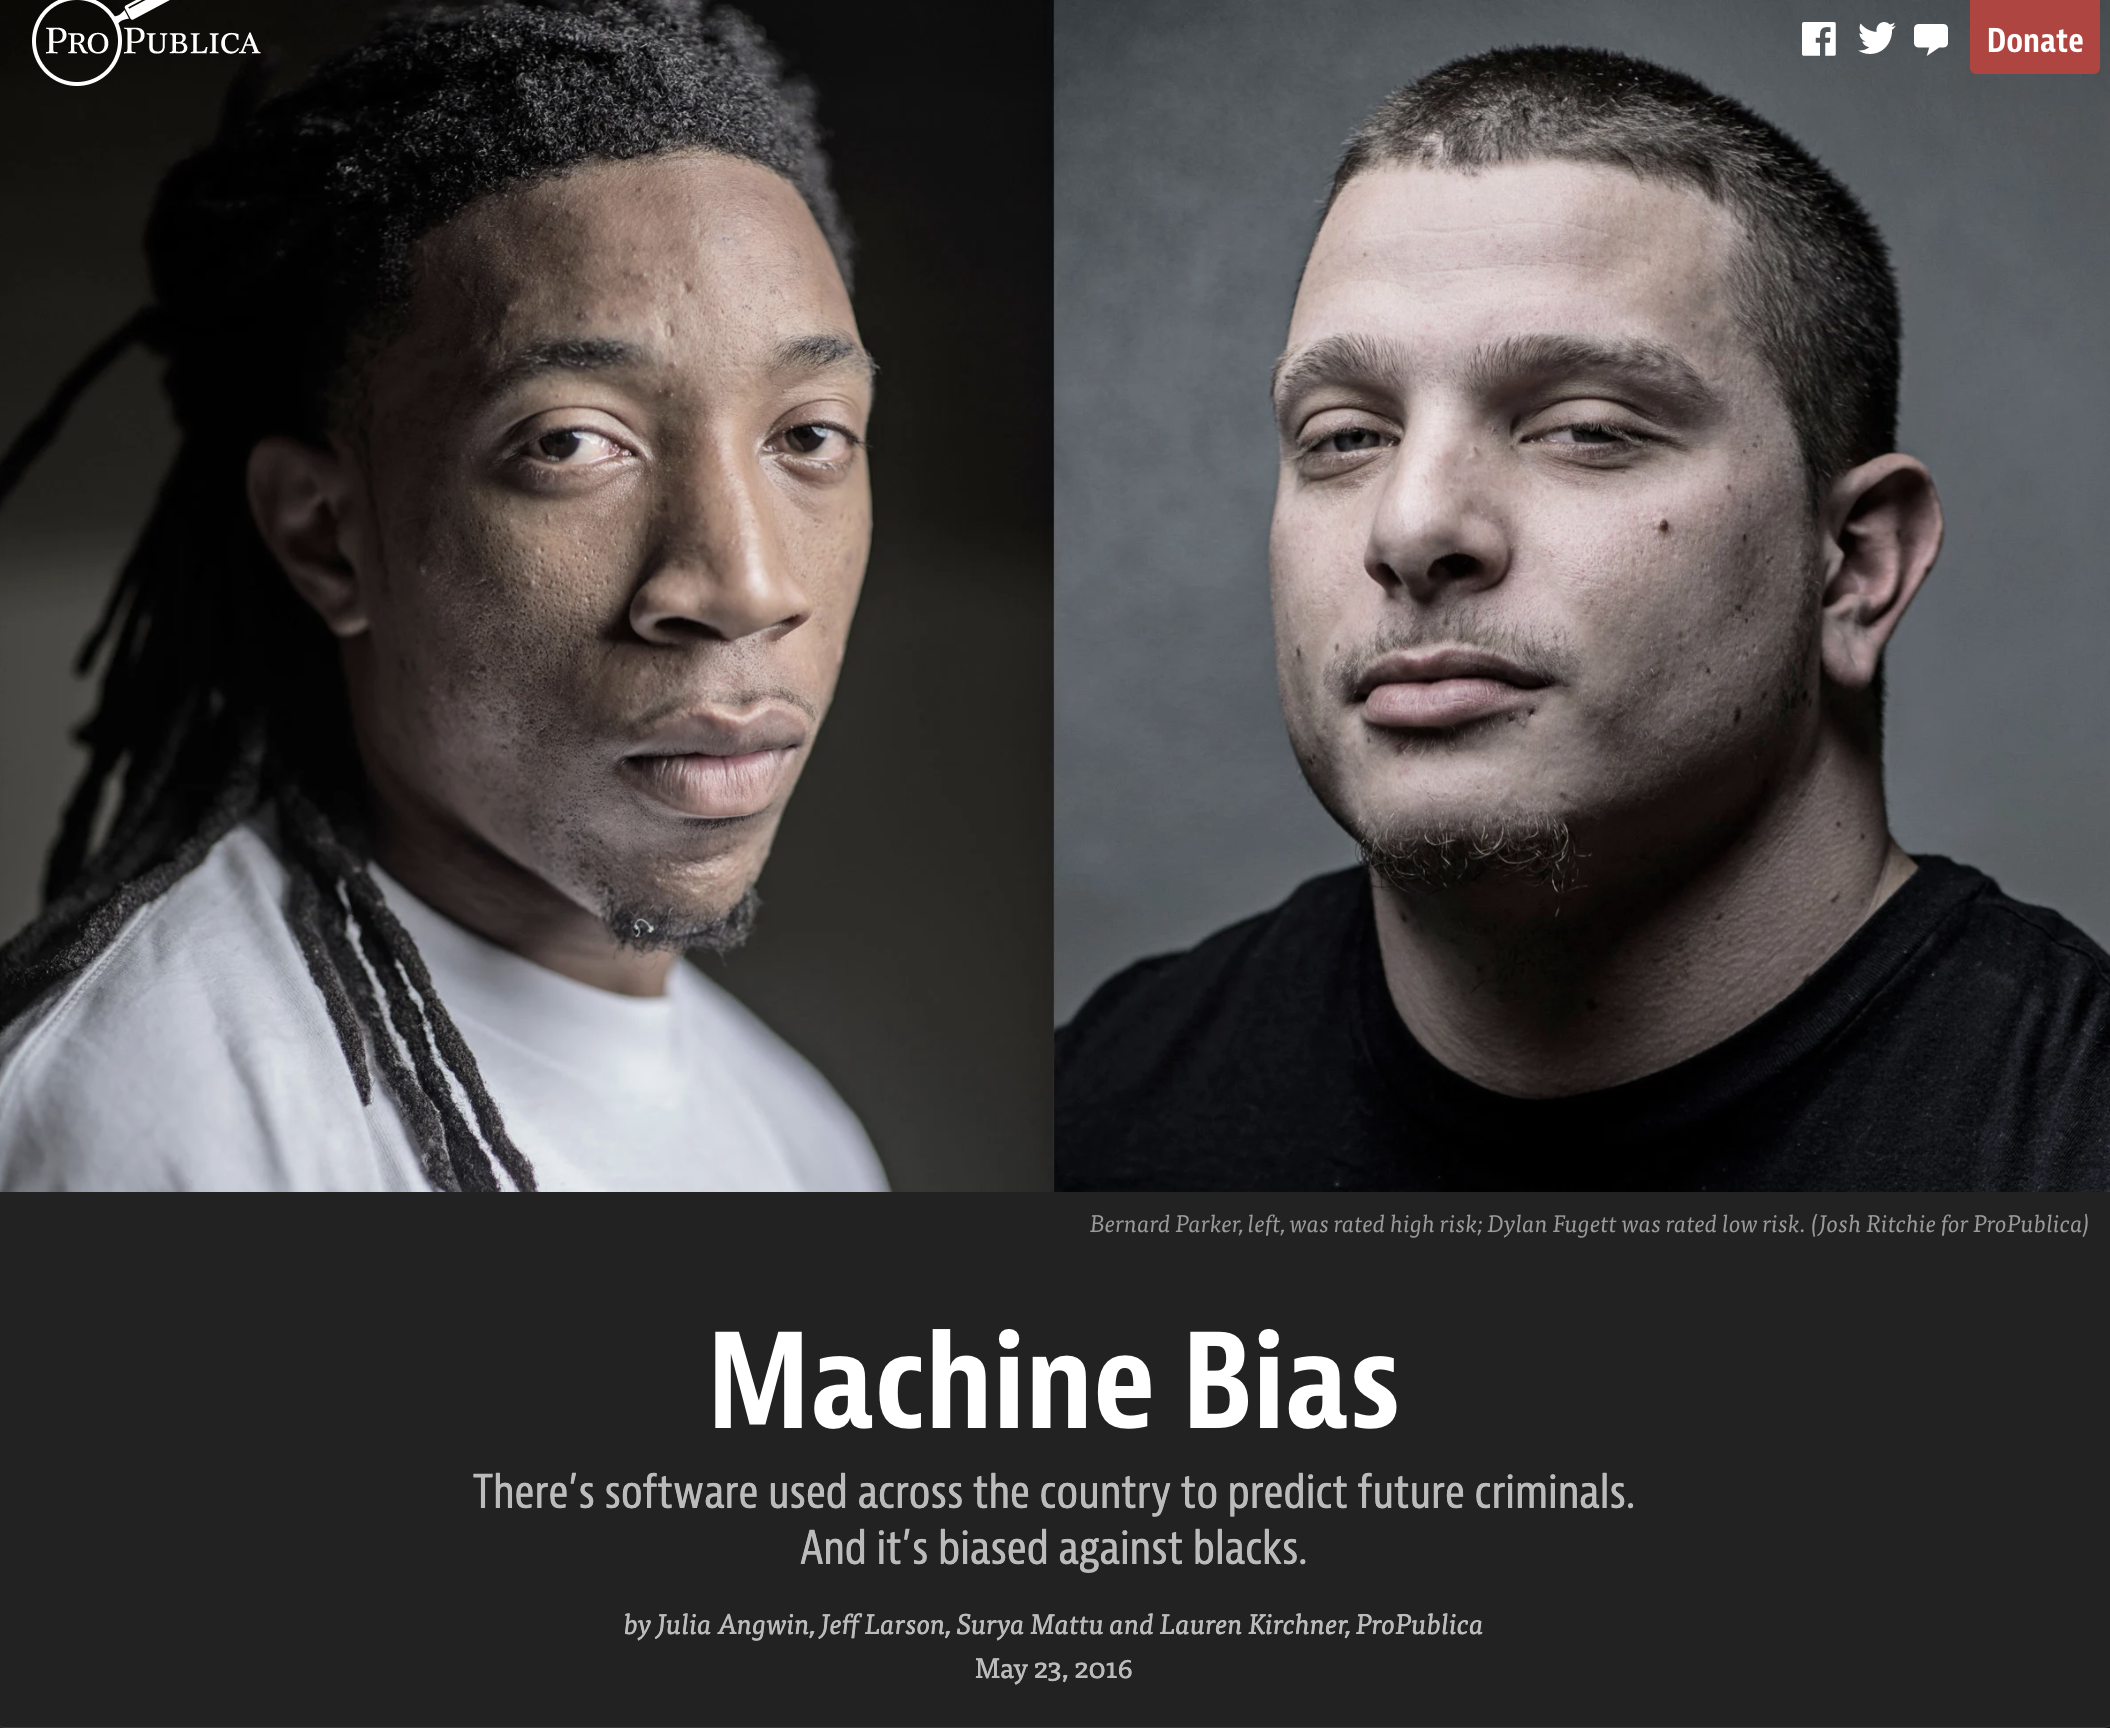
\includegraphics[width=0.7\textwidth,height=\textheight]{img/ethics-2.png}

~

\textbf{Discuss:}

\begin{enumerate}
\def\labelenumi{\arabic{enumi}.}
\item
  How might bias have entered the training datasets for these ML models, if the people labeling the data did not deliberately intend to exhibit prejudice against African Americans?
\item
  The ML models used to predict recidivism are imperfect and inherently prejudiced, but it is not clear whether it would be better to leave decisions of sentencing, bail amounts, and prisoner support services to individual humans in the court and penal systems. Would it be better to stop all use of ML evaluations, or should they be kept in place until better models are developed?
\item
  Returning to the beauty contest debacle. The attraction of a `robot jury' compelled people to seek out a single, simplistic definition of beauty, and to place all contestants on the same spectrum of beauty scores. Other than the racial bias baked into their model, what other problems is there with this endeavor? Articulate and enumerate as many as you can. What do those problems tell you about other ethical and humanistic dangers inherent to data science?
\end{enumerate}

\hypertarget{web-scraping-okcupid}{%
\subsection*{Web-scraping OKCupid}\label{web-scraping-okcupid}}
\addcontentsline{toc}{subsection}{Web-scraping OKCupid}

In 2016, Danish researchers used new web scraping and text mining software to inventory the user profiles of 60,000 users on the online dating site \href{https://fortune.com/2016/05/18/okcupid-data-research/}{OkCupid}. Their goal was to use this dataset to test for correlations between `cognitive ability' and sexual orientation, religious affinity, and other personality traits. They chose these user profiles because they were publicly available online to anyone who wanted to sign up for a free account with OKCupid.

When they published their paper, they included a spreadsheet of the 60,000 user profiles in the supplementary material for their article. They had removed the first and last names of the users, but kept everything else, including username, location, sexual orientation, religious orientation, sexual habits, relationship fidelity, drug use history, political views, and more.

The backlash was immediate. When asked why they did not attempt to deidentify or anonymize the data any further, the researchers responded that the data were already public. In the paper itself, the authors wrote: ``Some may object to the ethics of gathering and releasing this data \ldots{} However, all the data found in the dataset are or were already publicly available, so releasing this dataset merely represents it in a more useful form.''

~\\

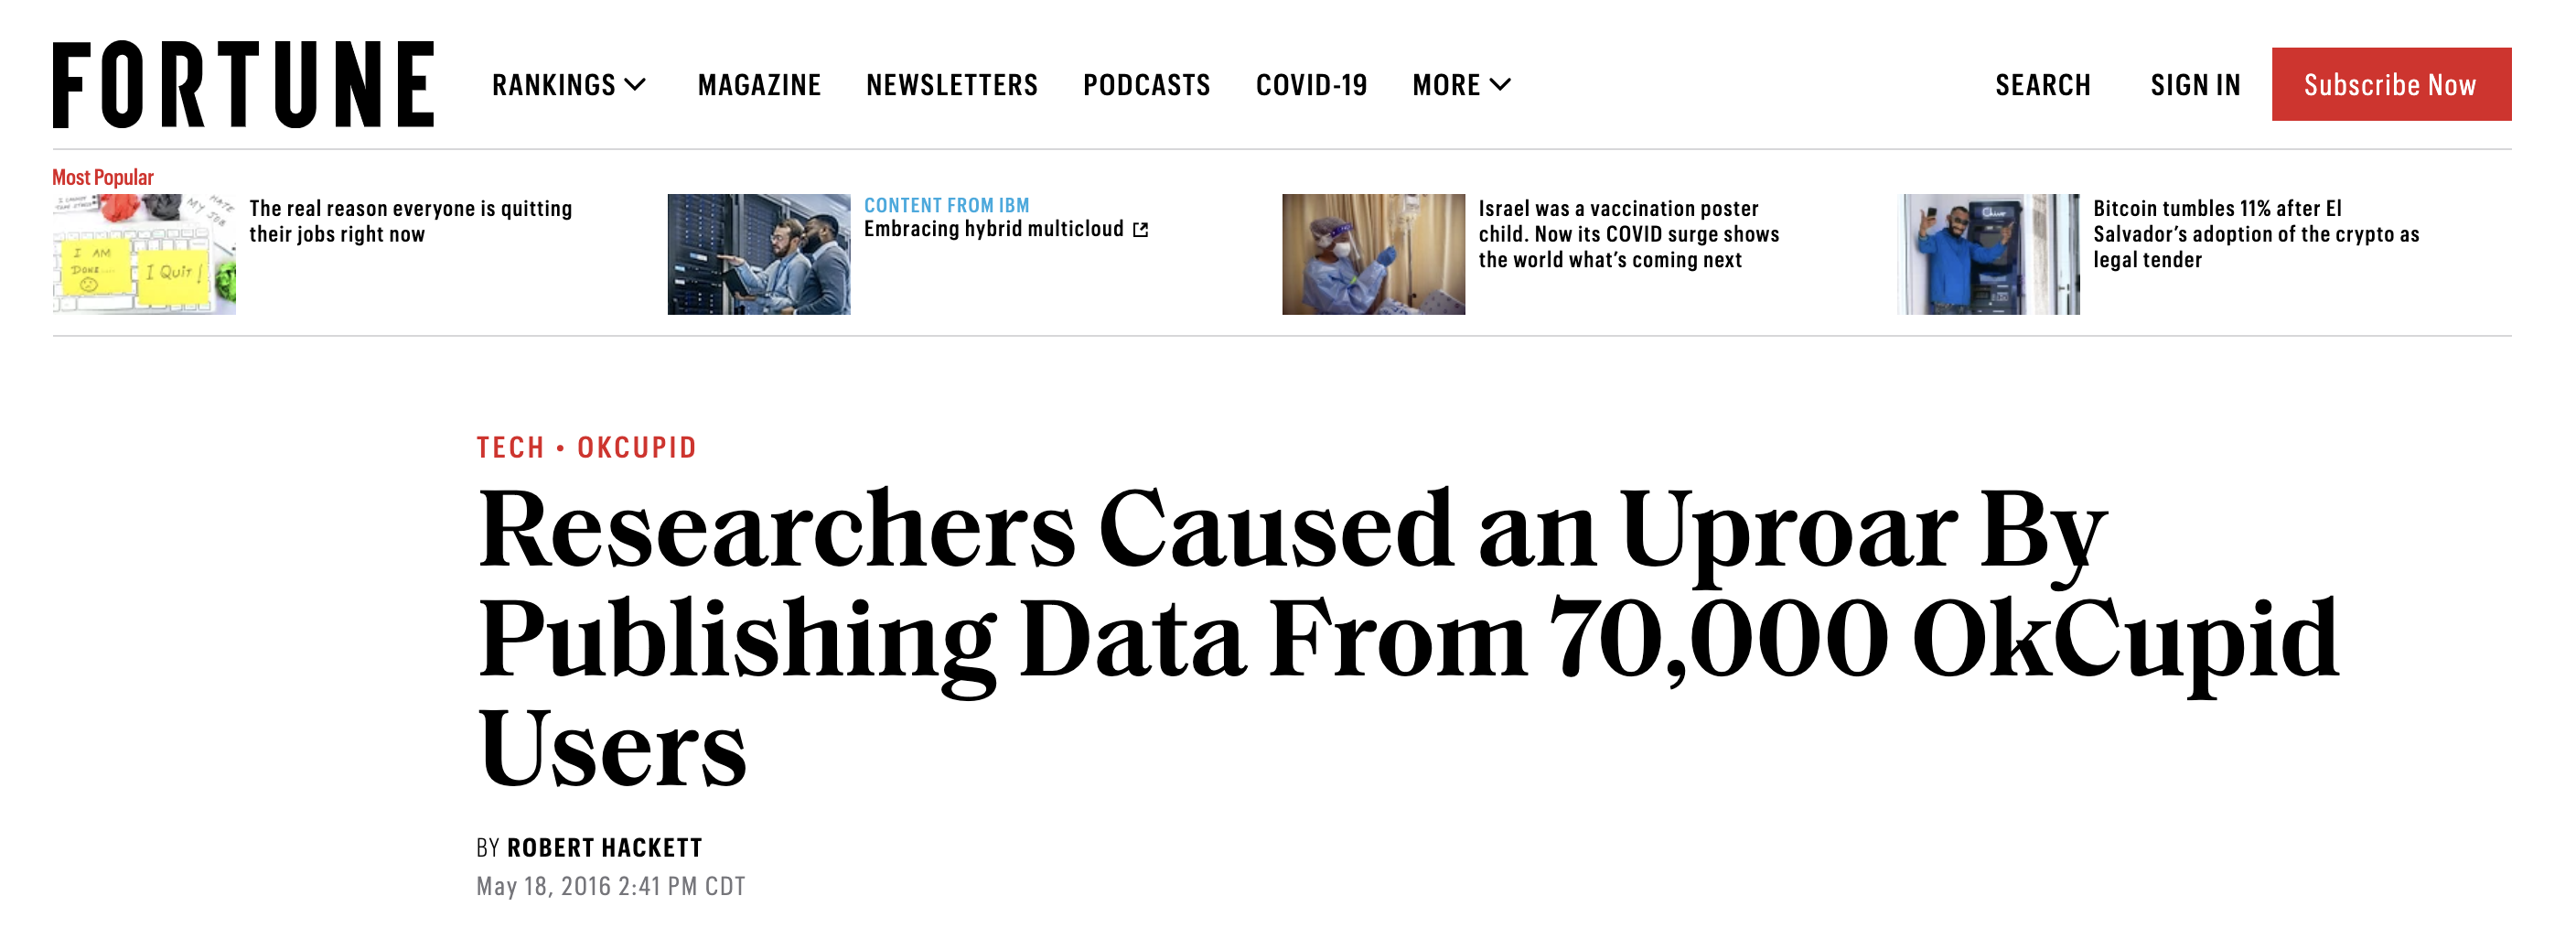
\includegraphics[width=0.8\textwidth,height=\textheight]{img/ethics-okcupid.png}

~

\textbf{Discuss:}

\begin{enumerate}
\def\labelenumi{\arabic{enumi}.}
\item
  What do you make of the authors' argument, that the data were already public, posted freely by the users themselves, so how can this be an issue of privacy or consent?
\item
  If you disagree with the authors' argument, explain how the users might reasonably object to the authors' actions.
\item
  What kind of risks did the authors impose upon the users of OKCupid? Are any of those risks new, or were they all present when the users decided to make a profile that could have been accessed by any other user?
\item
  Does it make an ethical difference that the authors accessed publicly available data in a novel way (web-scraping software) and to a much greater extent (harvesting 60,000 profiles at once) than individual users are typically able to do?
\item
  Does the software developer of the web-scraping tool bear any responsibility for this scandal? Does he have any ethical obligations regarding how his tool is used, and by whom?
\end{enumerate}

\hypertarget{more-scenarios}{%
\section*{More scenarios}\label{more-scenarios}}
\addcontentsline{toc}{section}{More scenarios}

\textbf{Airport screening}\\
A data scientist has come up with a model that prioritizes security screening at airports according to various passenger characteristics. If using `place of origin' as a predictor in this model improves the model's predictive performance at identifying passengers who are security threats, is it ethical to include that variable in the model and screen certain passengers disproportionately?

\textbf{Supporting struggling college students}\\
Your college has developed a model that predicts dropouts. It identifies students at high-risk of dropping out and alerts offices that can direct additional support and resources to these students. Your college has found that this model performs better when it includes the student's place of origin, sex, and race as predictors. Is it ethical to implement this model and divert resources accordingly?

\textbf{Robot cashiers}\\
Self-checkout stations in grocery stores are convenient, but they take jobs away from workers who may not have many other employable skill-sets. When you are checking out, is it more ethical to use the checkout aisles with human cashiers, even if the line is longer and going more slowly?

\textbf{Electric cars}\\
Cars running on fossil fuels are bad for the environment, but at least they can be serviced by car mechanics who don't necessarily need a college degree.

Electric cars reduce carbon emissions, but they are replacing car mechanics with computer scientists and softwar engineers, all of which require extensive undergradate and post-graduate education. Are electric cars a net social good?

\textbf{Smartphone app for monitoring cough}\\
A tech start-up has developed an app that can track the prevalence of cough in a network of smartphones. Cough is an important indicator of disease, and cough also helps to spread certain diseases more quickly, such as TB and COVID-19. This app has great potential to help public health officers in the fight against some of the deadliest respiratory diseases. The app works thanks to sophisticated machine learning algorithm for detecting coughs within continuous recordings. That algorithm is currently private and propriety. Do you agree that this cough monitoring app is a good idea, and that public health officials should promote its use?

\textbf{Automated suicide prevention system}\\
A large internet search engine has developed a model that can predict whether someone is likely to inflict self-harm or attempt suicide based upon their recent search history. This model is 75\% accurate. This company would like to set up an automatic emergency alert system, in which local social service providers are notified about at-risk users in their area. They want to automatically enroll users in this service. Is this an ethical feature to add to their product?

\textbf{Malaria medicine distribution}\\
Your company is trying to distribute a new malaria medicine in a remote region of Africa without primary care clinics, where tens of thousands people die from malaria each year. This medicine is highly effective, but it is also known to cause birth complications. You need to ensure that it is not administered to pregnant women. Your team's plan is to go door to door and distribute the medicine to women who say they aren't pregnant.

But in this region, cultural attitudes to pregnancy, and the notion of sharing your pregnancy status with a stranger, are very sensitive. Daughters and wives may not feel safe to answer such questions truthfully.

Your team has to choose between (1) taking women's responses at their word, (2) avoiding the pregnancy issue by only distributing it to men, (3) not distributing the medicine at all, (4) some as-yet-unknown solution. What do you do?

\textbf{User accountability}\\
Let's say that you have disagreed with one or more of the claims about social media in the `Warm-Up Scenarios' section above. Is it ethical for you to continue to use Google, Instagram, or Facebook?

\hypertarget{dataviz}{%
\chapter{Visualizing data}\label{dataviz}}

This course will focus heavily on visualizing data in plots, maps, and dashboards. If there is anything you take from this course, it will be this: you will be able to take data and make some pretty pictures. \emph{And that's not trivial!}

Why? Because \textbf{humans are wired to process information through \emph{pictures}.} We can translate images into meaning with amazing speed.

\hypertarget{the-value-of-data-viz}{%
\section*{\texorpdfstring{The value of \emph{data viz}}{The value of data viz}}\label{the-value-of-data-viz}}
\addcontentsline{toc}{section}{The value of \emph{data viz}}

This screenshot, from David McCandless's \href{https://www.youtube.com/watch?v=5Zg-C8AAIGg}{TED talk} about the beauty of data visualization, depicts how quickly each of our senses can process information.

~\\

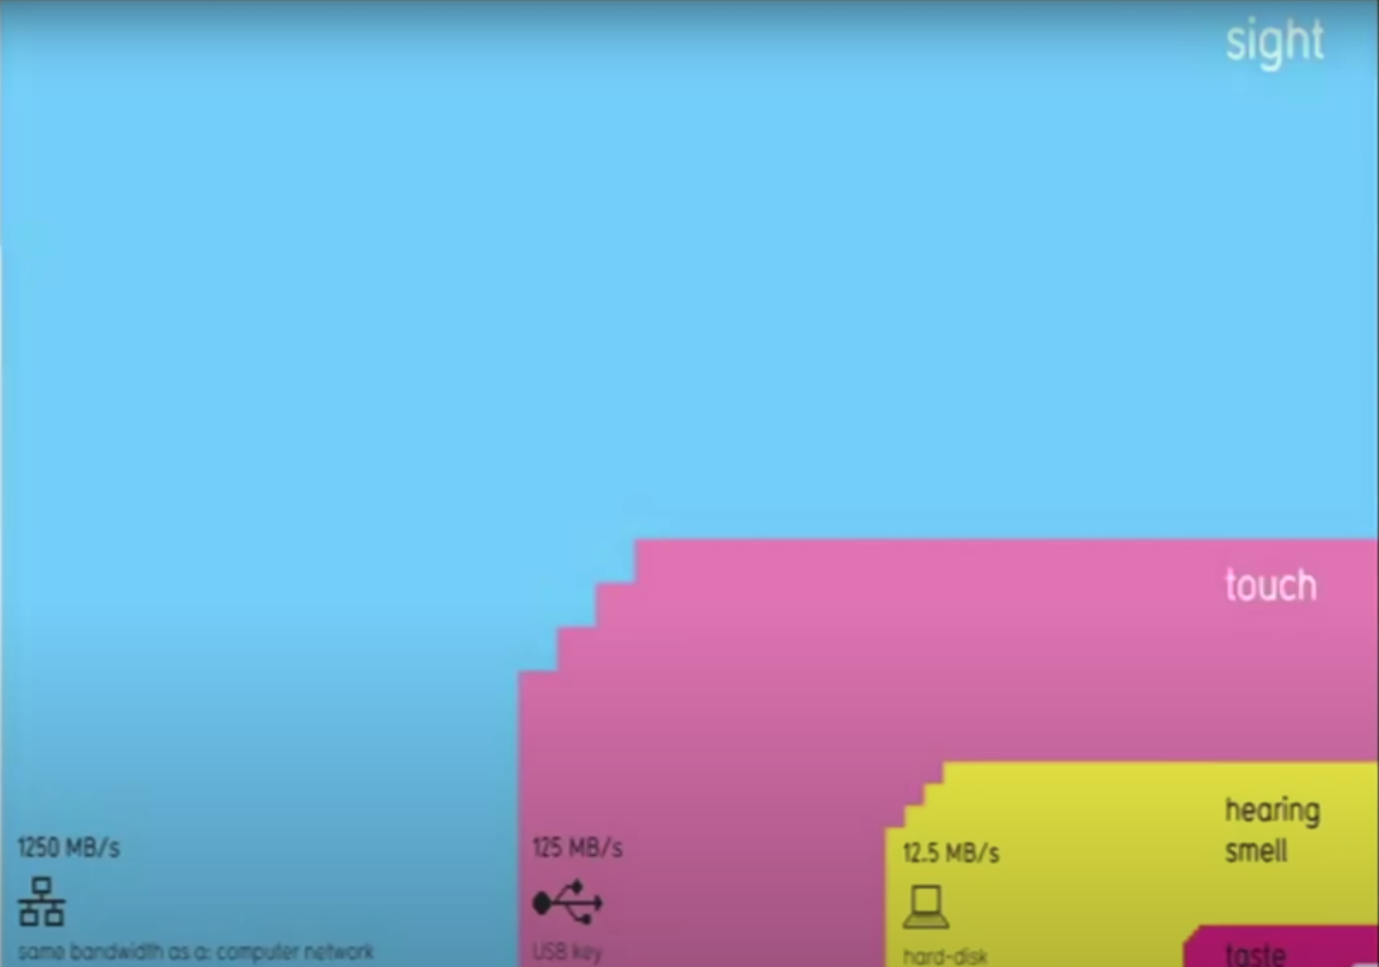
\includegraphics[width=0.7\textwidth,height=\textheight]{img/vis0.png}

~

\textbf{This plot's punchline:} When we process data with our eyes -- with \emph{pictures} -- we can take in a lot of information all at once.

\textbf{Let's try this out with an example.} Below this paragraph is another paragraph describing a painting. Try this: when you get to the end of \emph{this} sentence, click as directed, look at the paragraph for just \emph{one second}, then click on the link after the paragraph. Click here!

\textbf{One-second paragraph:}

\emph{Fog rises from the evergreen forest of a distance mountain range. A whitewater creek cascades down a streambed with large, rounded boulders, arriving at a broad flatwater pool where ducks are milling. There is one group of four and another group of two. On the shore near the ducks, a wooden dinghy is tied up to a small dock with eight pilings. The dock lead to a path through more round peddles and tall grass, past a chair and a fire ring, and continues uphill to a small cabin. The evening sun and sparse fairweather clouds are reflected in the cabin's large, multi-paned windows under the small front porch. A cobblestone chimney on the side of the cabin has a whisp of smoke rising from it. The steep roof implies that this cabin is designed to withstand heavy snow. Tall evergreens tower over the diminutive cabin; the cabin seems to be placed up against a forested hillside. There are only a few deciduous trees in view, and their leaf colors -- combined with the lack of snow in the distant mountains -- imply that the time of year is early fall.}

\textbf{Click here}

~

Now try to answer these simple questions:

\begin{itemize}
\item
  What was this a painting of, in general? Can you describe the scene?
\item
  What details do you recall?
\end{itemize}

OK. Try this next: the actual painting is at the very end of this chapter. At the end of this sentence, click as directoed to see it, look at the painting for just \emph{one second}, then come back to this point in the module. Go to the painting!

~

Now try to answer those same questions above. What was this a painting of? Did you catch any more details? Was there anything in the water? Was there smoke coming out of the chimney? What time of day was it?

Which type of visual information was easier for you to process quickly? Text, or a picture?

Think about the profound \emph{differences} in these two forms of visual communication:

When we read text, we are working outward, from individual details to the big picture: we process each individual word, understand their individual meanings, understand their meanings in the context of each individual sentence, then use all of the information to step back and imagine the scene based on the details.

In contrast, when we look at a picture, we are working inward, from the big picture down to the details. We understand the scene first, then we start exploring the finer points. And, since each finer point is interpreted from within the context of the bigger picture, we can make sense of the details much more efficiently.

Pictures communicate data. \textbf{This is why data \emph{science} and data \emph{visualization} nearly always go hand in hand.}

Data scientists use visualizations both to communicate their insights externally, e.g., to the public in a \emph{Twitter} post, but also internally: when they are working with the data themselves. A data scientist's workflow is peppered with data visualization, because -- again -- visualizing your data is the most effective way of making sense of it: Download the data, then visualize it. Do something to the data, then visualize what you've done. Repeat, then visualize, then repeat again.

The point here is that great data visualizations are not simply pretty. Much more importantly, they are \emph{effective} too. They are the best means you have of conveying insights from your data to someone else.

\textbf{A final thought:} Keep in mind that plots can be effective and misleading at the same time. There is a politics to plots and maps; they can have agendas, and they can manipulate viewers into interpreting the data in certain ways. So, it is incomplete for us to say simply that a good plot is an effective plot. Here's a better definition: \emph{a good plot is one that is both effective and fair.}

So, when you are viewing other people's plots and making plots of your own, keep these five rules in mind:

\begin{enumerate}
\def\labelenumi{\arabic{enumi}.}
\item
  A bad plot is an ineffective one, even if it is beautiful.
\item
  A good plot is an effective plot.
\item
  A great plot is one that is both effective \emph{and} beautiful.
\item
  If you ever have to make a trade-off between effectiveness and beauty, sacrifice beauty.
\item
  Any plot that misleads or manipulates the viewer is bad, no matter how effective or beautiful it is.
\end{enumerate}

Before you begin evaluating the plots in the gallery below, enjoy this excellent talk by the Egyptian data scientist, \textbf{David McCandless}, about the \textbf{beauty of data visualization} (link \href{https://www.youtube.com/watch?v=5Zg-C8AAIGg}{here}).

~

\hypertarget{plot-gallery}{%
\section*{Plot gallery}\label{plot-gallery}}
\addcontentsline{toc}{section}{Plot gallery}

What follows is a gallery of plots: some good, some bad, and some ugly too. Let's use these to explore what works and what doesn't. For each plot, ask yourself three questions:

\begin{itemize}
\item
  What makes this plot good (as in, effective and not misleading)?
\item
  What makes this plot bad (ineffective and/or misleading)? How could the plot be improved?
\item
  What might make this plot prettier?
\end{itemize}

The point of this is not to make fun of others for their plots. The point is to learn from their choices. Because plot technique matters. Data science is about communication, action, and impact. You will spend so much time working on an analysis, and you are gonna go through all the work of making a plot. What a shame if the end product undermines all of that hard work!

~

~

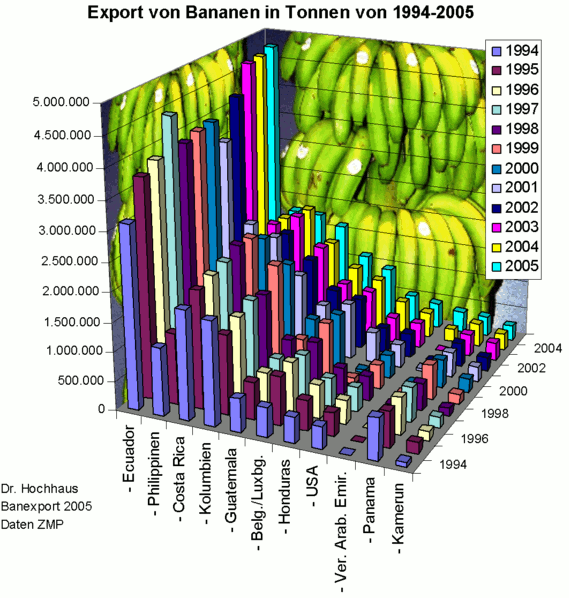
\includegraphics{img/vis1.png}

~

\begin{itemize}
\tightlist
\item
  \textbf{Good:} Frankly, there is not much good about this plot. Yes, it has a lot of information, but this crosses the line into information overload. It is so convoluted and difficult to interpret that we quickly lose interest in spending time exploring its details.\\
\item
  \textbf{Bad:} The 3D perspective (1) makes it almost impossible to compare bar heights, (2) causes alot of the bars in the back to be hidden, and (3) adds needless complexity.\\
\item
  \textbf{Bad:} The 3D perspective makes it almost impossible to compare bar heights.
\item
  \textbf{Bad:} The colors representing each year do not follow a logical sequential flow; years are sequential, and colors can be too (think the ROYGBIV rainbow sequence).\\
\item
  \textbf{Ugly:} The bananas! Sure, this plot has to do with banana exports, but those banana pictures don't represent anything at all about the data and they make everything else convoluted. Plus, it's cheesy.
\end{itemize}

~\\

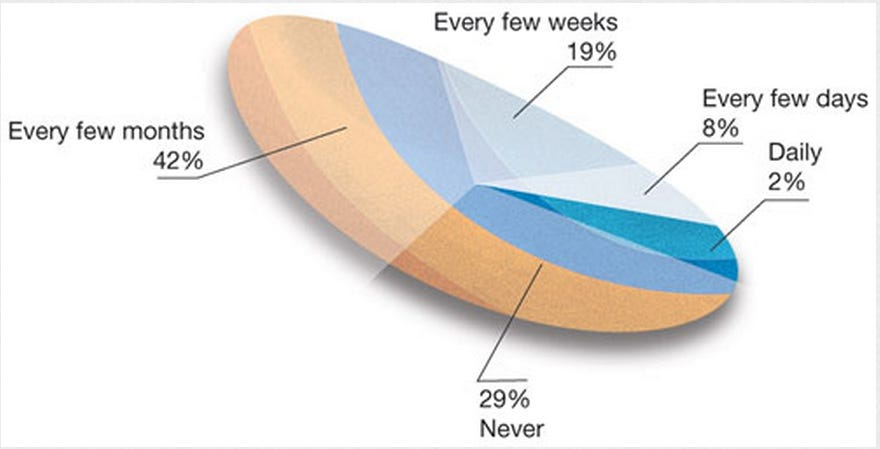
\includegraphics[width=0.7\textwidth,height=\textheight]{img/vis2.jpeg}

~

We don't think this plot is good or pretty.

\begin{itemize}
\tightlist
\item
  \textbf{Bad:} This is an unfamiliar plot format; is it a pie chart? A blood platelet? A pickle?
\item
  \textbf{Bad / Ugly:} Why is it lopsided or rotated? That has nothing to do with the data.
\item
  \textbf{Bad:} What is this plot even about? There are no context clues whatsoever. Titles and labels, in moderation, can be really helpful.
\item
  \textbf{Bad / Ugly:} What are the colors representing? They seem to have no relation at all to the pie slices. Very confusing.
\item
  \textbf{Bad:} The slices do not seem to represent the percentages accurately. The 8\% slice does not look four times larger than the 2\% slice.
\end{itemize}

~\\

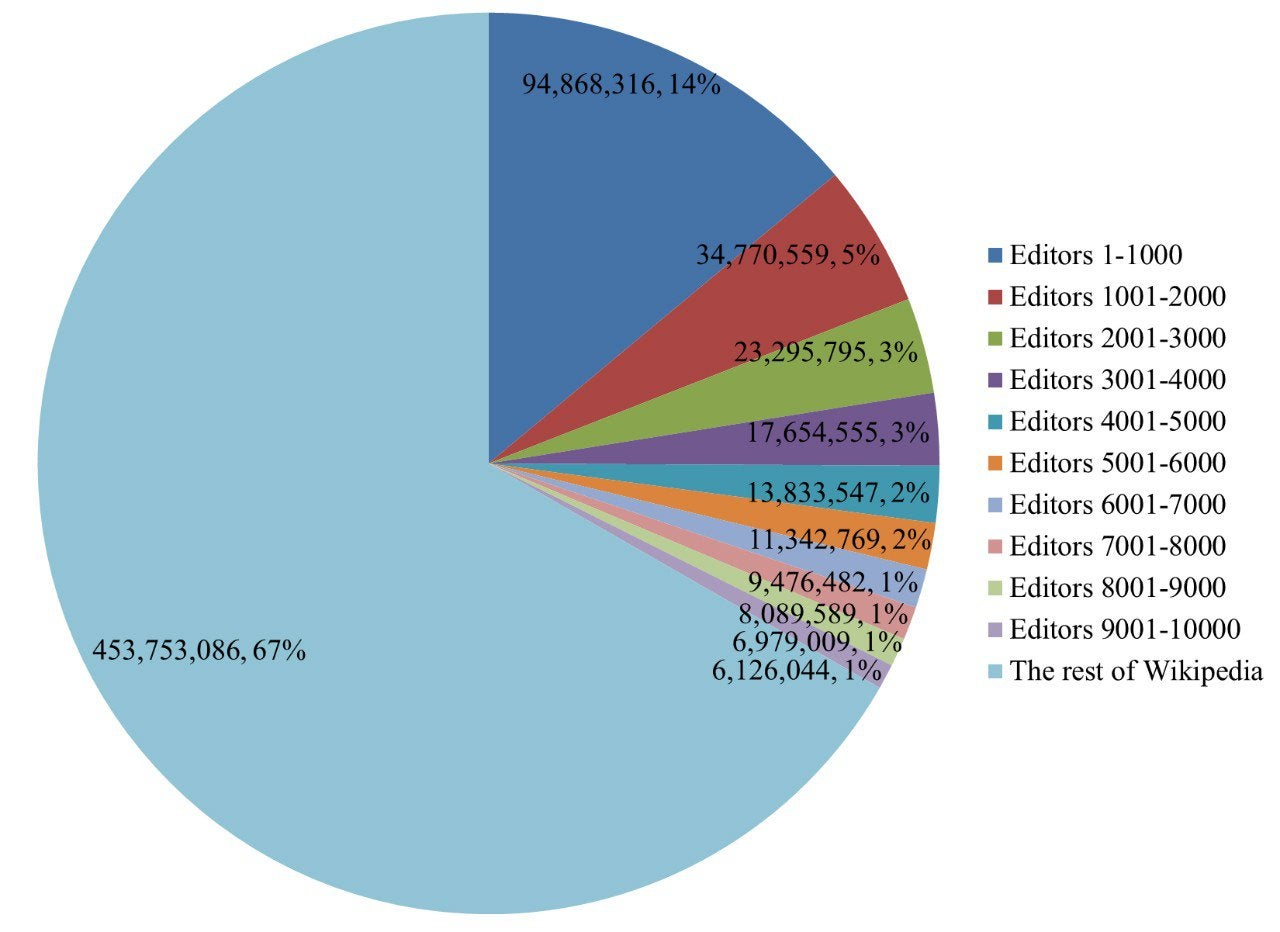
\includegraphics[width=0.7\textwidth,height=\textheight]{img/vis3.jpg}

~

Here is another pie chart that isn't very effective.

\begin{itemize}
\tightlist
\item
  \textbf{Bad:} Lots of significant digits in these number. Instead of forcing viewers to read numbers like 453,753,086, why not display 454 M?\\
\item
  \textbf{Bad:} The percentages next to the other numbers make it even harder to read.
\item
  \textbf{Bad:} Superimposing text on top of the pie sclices makes it impossible to use the slices for their intended purpose: visually comparing the size of subgroups in the data.
\item
  \textbf{Bad:} There are so many color-coded slices that it takes far too long to understand the details.
\item
  \textbf{Bad:} One reason it takes so long is that the text is redundant: don't put a lot of text on the pie \emph{and} put a lot of text in your legend. Figure out a way to point to each pie slice with a line, then have all the info for that slice in the same spot.\\
\item
  \textbf{Bad / Ugly:} The dark text on top of dark colors is hard to read.
\end{itemize}

Pie charts are \emph{super} common in media, but they are actually an infamously bad form of data visualization. That's because the human eye is much worse at comparing \emph{areas}, such as the size of a pie slice, than they are at comparing \emph{heights}. To make matters worse, we are worse at comparing areas for non-rectangular shapes, like a pie slice, than for squares or rectangles. So: avoid pie charts.

~\\

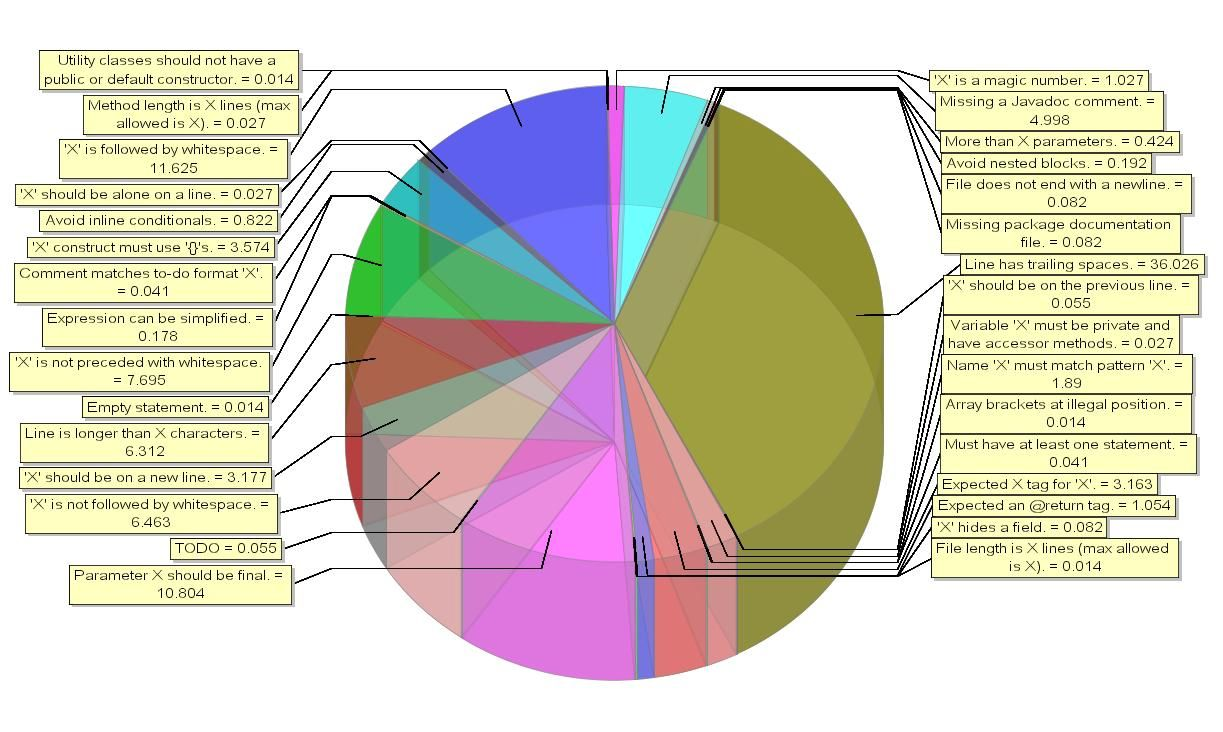
\includegraphics[width=0.8\textwidth,height=\textheight]{img/vis6.jpg}

~

\begin{itemize}
\tightlist
\item
  \textbf{Bad:} Pie chart.
\item
  \textbf{Bad:} There is no reason for this to be 3D. The third dimension has nothing to do with the data.
\item
  \textbf{Bad:} There is no reason for this to be semi-transparent. It just makes everything even more convoluted.
\item
  \textbf{Bad:} The text is way too small to read.
\item
  \textbf{Bad:} On a related note, there is way too much text.\\
\item
  \textbf{Bad / Ugly:} The yellow text boxes and dark lines around them add uninformative junk to this plot. If all lines unrelated to data or labels were removed, this chart would be more intelligible.
\end{itemize}

~\\

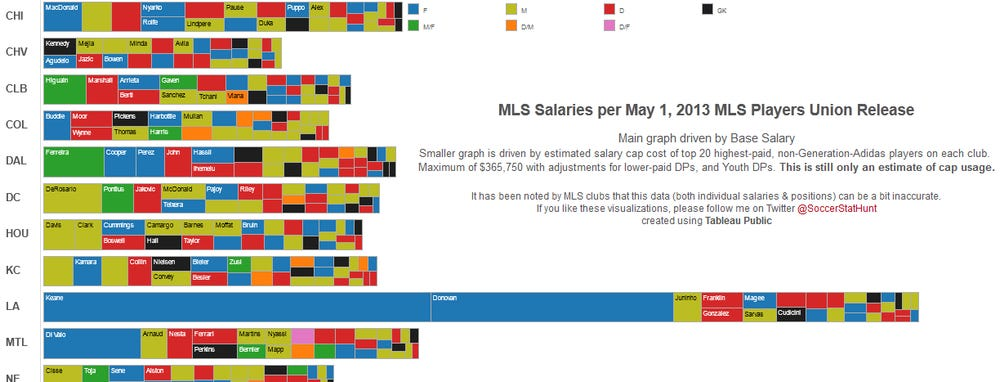
\includegraphics{img/vis7.jpeg}

~

\begin{itemize}
\tightlist
\item
  \textbf{Bad:} Information overload.
\item
  \textbf{Bad:} It is not clear whether the repeat use of colors in each row conveys any meaning, or if it is just a random recycling of colors.
\item
  \textbf{Bad:} The text is too small to read.\\
\item
  \textbf{Bad:} Abbreviations are not explained.
\end{itemize}

~\\

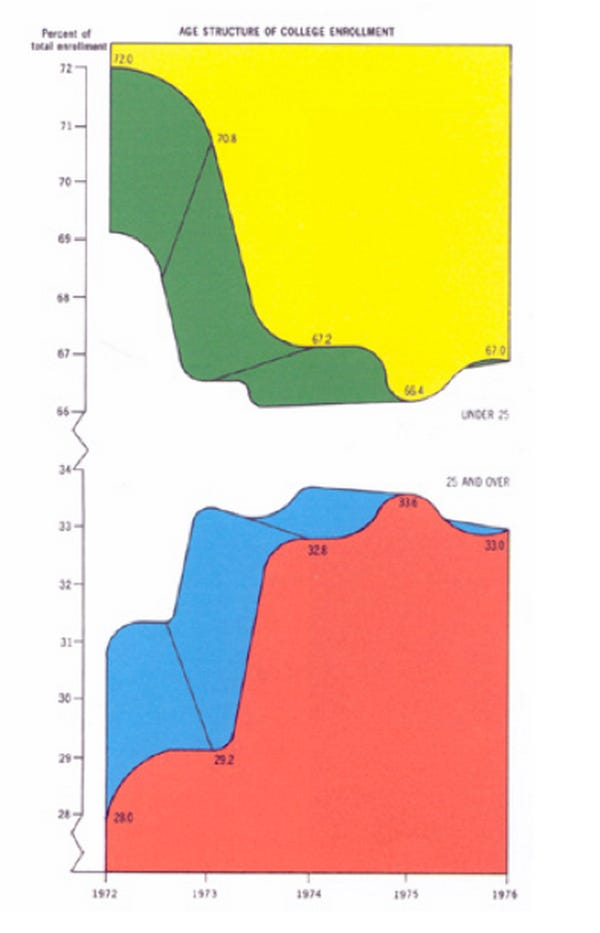
\includegraphics[width=0.6\textwidth,height=\textheight]{img/vis8.jpeg}

~

\begin{itemize}
\tightlist
\item
  \textbf{Bad:} The text is very small.
\item
  \textbf{Bad / Ugly:} The third dimension, with a weird perspective effect added, has nothing to do with the data and makes this plot difficult to understand. Should you pay attention to the edge in the distance or the line in the foreground? Are they the same?\\
\item
  \textbf{Bad:} The y axis is crazy! (1) The scale break is confusing. (2) The attempt to plot these two subgroups as separate trends belies the fact that one is just the remainder of the other: the two curves sum to 100\%. (3) By attempting to place the two trends on the same proportional scale, this plot gives the visual impression that the changes over time are really extreme.
\item
  \textbf{Bad:} The trend lines are unnecessarily curved. The plot's authors probably only have data for each semester, but smoothed lines give the impression that they have more data.
\end{itemize}

~\\

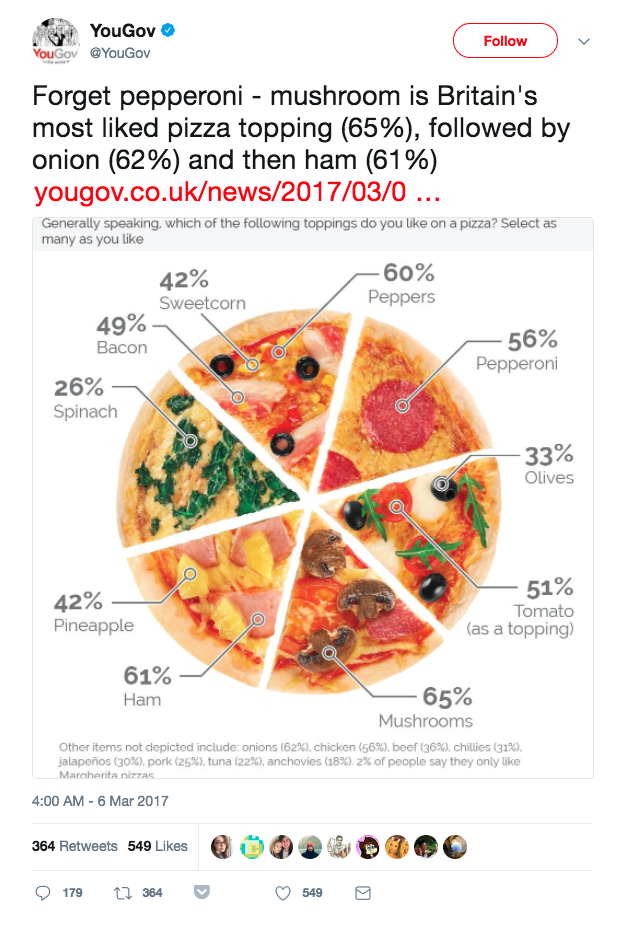
\includegraphics[width=0.7\textwidth,height=\textheight]{img/vis9.png}

~

\begin{itemize}
\tightlist
\item
  \textbf{Bad:} These percentages sum to more than 100\%. That needs to be explained, or avoided.\\
\item
  \textbf{Bad:} The use of a pizza pie, though creative, implies that the size of the pie slices will have something to do with the data. They don't.
\item
  \textbf{Bad:} Check out the fine print on the bottom. Several toppings were left off this chart, and some of them were quite popular; for example, onions had 62\% popularity and chicken was 56\% popular. Why are they not on this chart but spinach (26\%) is? The arbitrary exclusion of categories should immediately make viewers suspicious: how are these decisions being made?
\end{itemize}

~\\

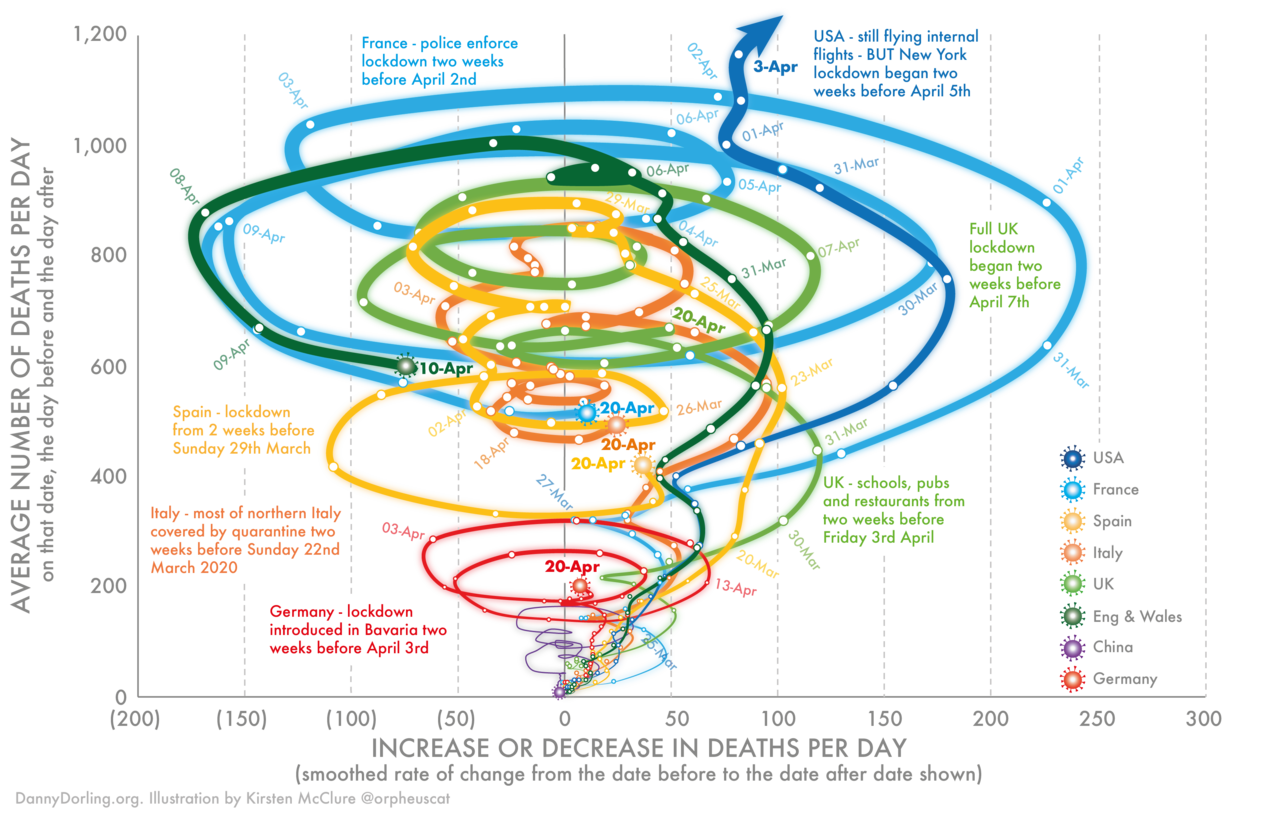
\includegraphics{img/vis10.png}

~

This is another case of information overload, and another case of a creative visualization that doesn't really help us make sense of what's going on. If we wanted to understand the take-a-way message or punchline from this plot, we're not sure we'd be able to. We could stare at this for minutes and still not understand what we are looking at, and it is so complicated that we would rather ignore this plot than go through that effort.

~\\

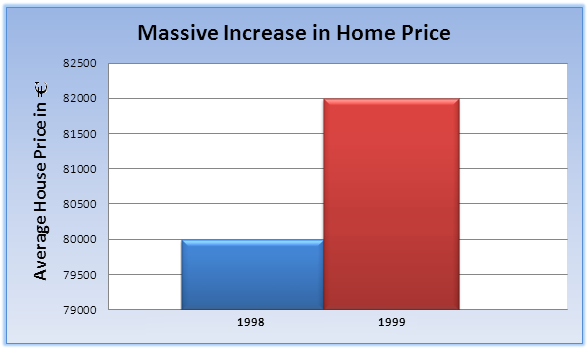
\includegraphics{img/vis11.png}

~

\begin{itemize}
\item
  \textbf{Bad:} The y axis range makes the difference in home prices sound a lot larger than it actually is. Based on the height of these two bars, you would expect the 1999 price to be 3x the the 1998 price when, in actuality, it is larger by 2.5\%.
\item
  \textbf{Bad:} The use of qualifiers such as ``Massive'' is generally discouraged. It's a little too controlling. Let the viewers make up their own minds about which differences are substantial and which are trivial.
\end{itemize}

These two notes are classic indicators of misleading or agenda-driven data visualization.

~\\

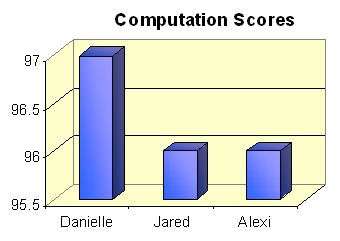
\includegraphics{img/vis12.jpg}

~

This is another example of manipulating perception with a sneaky y-axis range.

Also, like the examples above, this plot doesn't have to be 3D. The height has a meaning, but what does the depth mean? It is junk, in the sense that it does not add meaning.

~\\

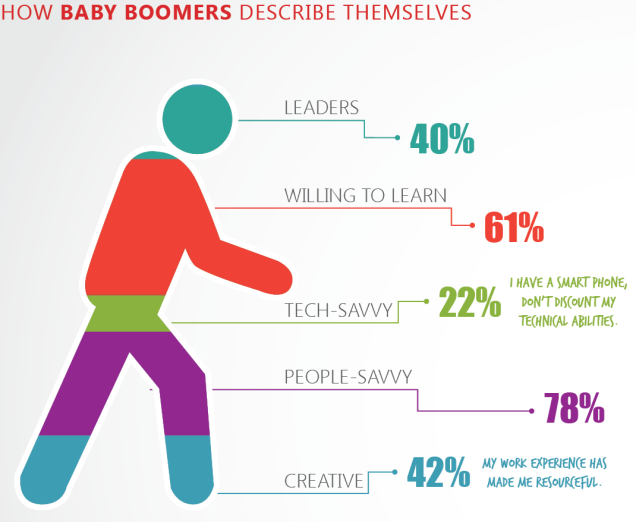
\includegraphics[width=0.75\textwidth,height=\textheight]{img/vis12.png}

~

\begin{itemize}
\item
  \textbf{Bad:} These percentages sum to more than 100\%. That needs to be explained, or avoided.
\item
  \textbf{Bad:} The rationale for ordering of the categories is not clear. They are not ranked by percentage. Are they supposed to correspond to the body part being pointed to in the figure? Should crotch equal `tech-savvy'?
\item
  \textbf{Bad:} The geometric shape itself (the person figure) does not help at all in visualizing the percentages. Can you compare the area of the feet and the area of the head? The fact that they provide the actual numbers in large bold font suggests that they knew the figure would not be useful as a picture.
\end{itemize}

~\\

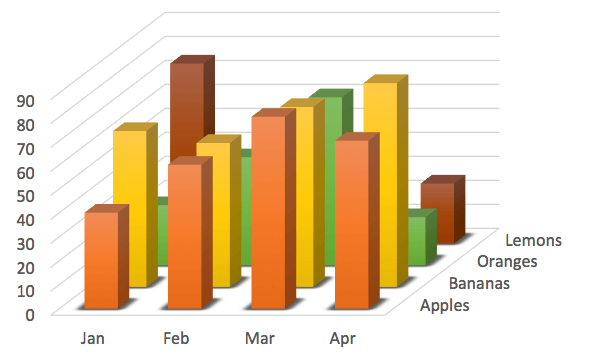
\includegraphics{img/vis13.png}

~

\begin{itemize}
\tightlist
\item
  \textbf{Bad:} Some data are completely obscured. What is happening to lemons in February and March?\\
\item
  \textbf{Bad:} Like the infamous banana plot above, the 3D perspective here makes it almost impossible to compare bar heights and adds needless complexity.
\end{itemize}

~\\

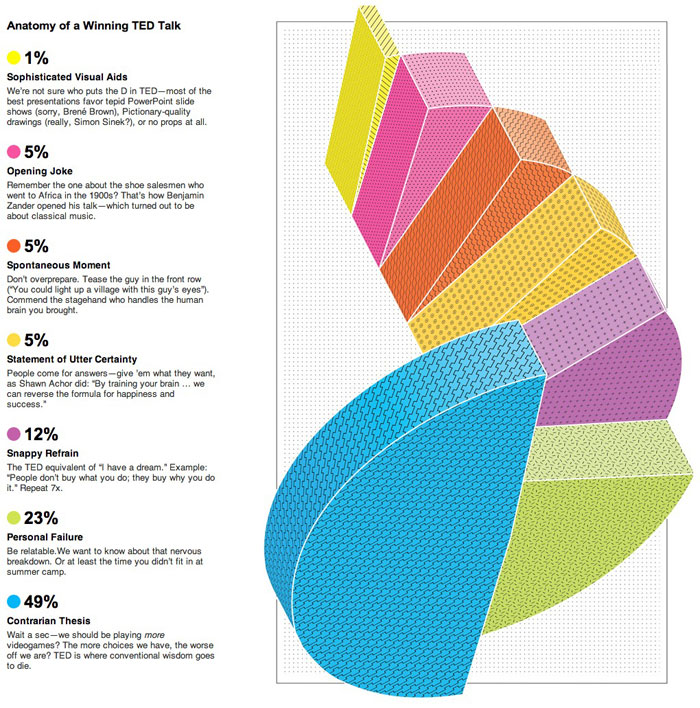
\includegraphics[width=0.8\textwidth,height=\textheight]{img/vis15.jpg}

~

\begin{itemize}
\tightlist
\item
  \textbf{Bad / Ugly:} The contortion of this pie chart into a spiraling 3D object is confusing and gratuitous.
\item
  \textbf{Bad / Ugly:} Some colors are very similar to each other.\\
\item
  \textbf{Bad:} Pie chart!
\end{itemize}

~\\

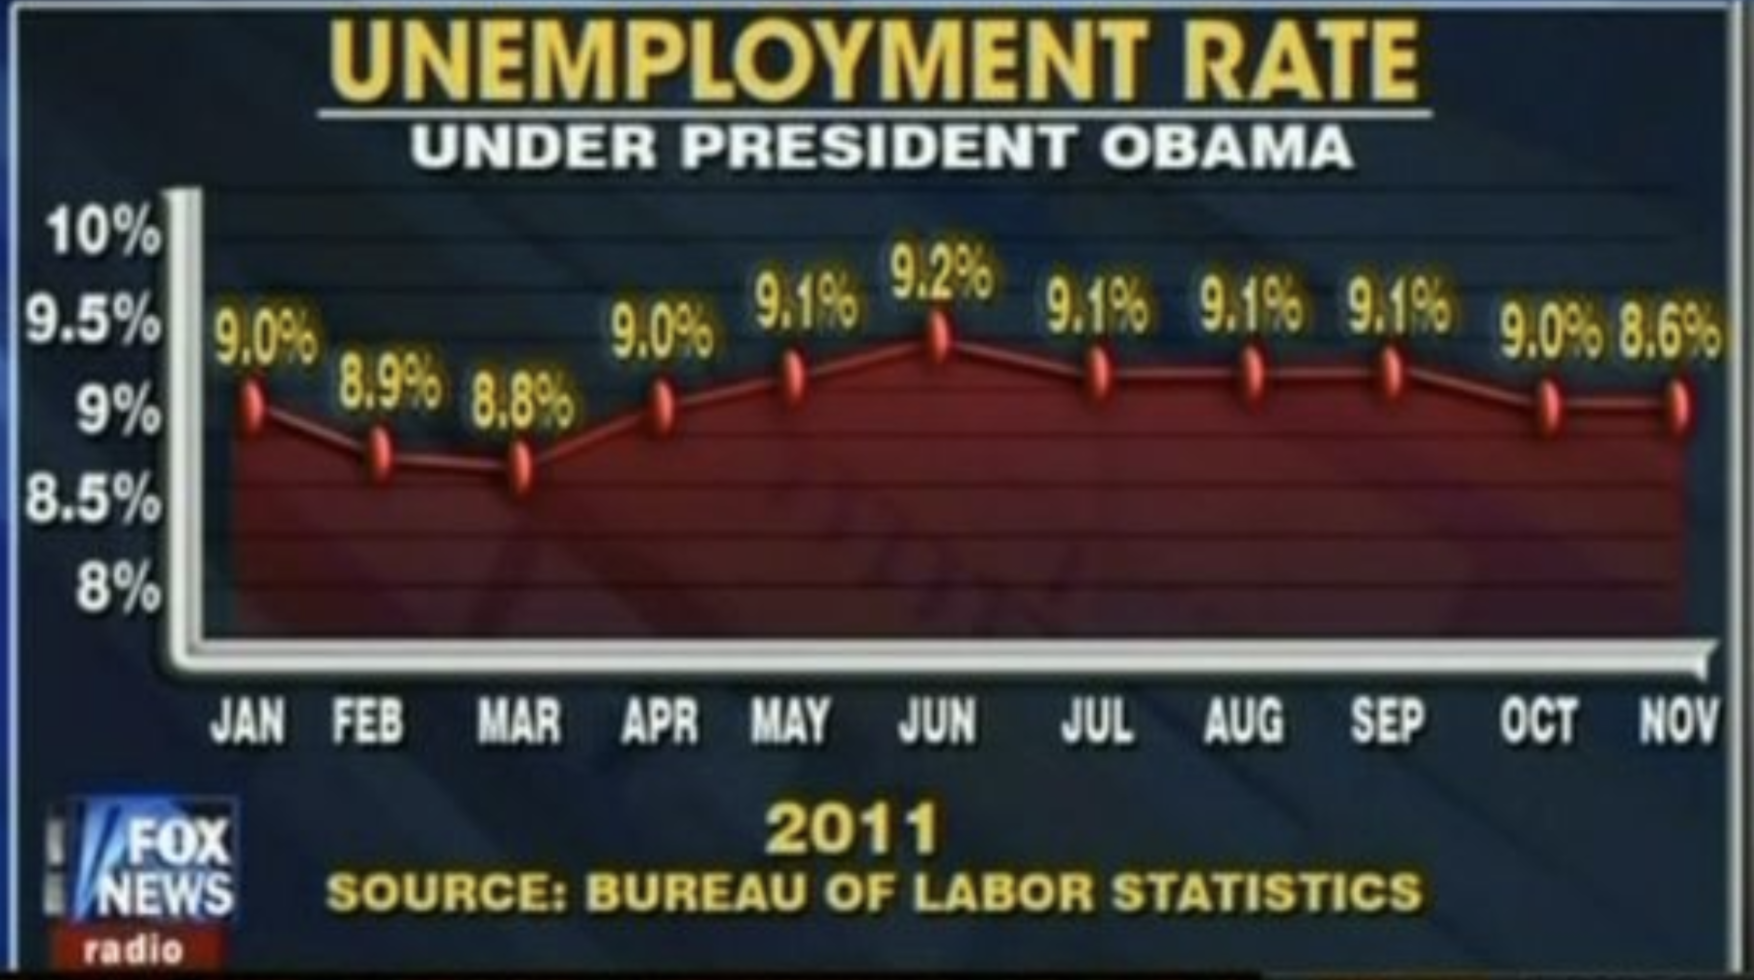
\includegraphics[width=0.75\textwidth,height=\textheight]{img/vis16.png}

~

\begin{itemize}
\tightlist
\item
  \textbf{Bad:} The small y axis range exagerrates changes in the unemployment rate.
\item
  \textbf{Bad:} The final data point on this plot is wrong! 8.6\% should not be at the same height as 9.0\%.
\item
  \textbf{Bad:} The title of this plot implies that the data will show unemployment trends throughout the Obama administration, which began in 2009, but this data is for 2011 only.
\end{itemize}

~\\

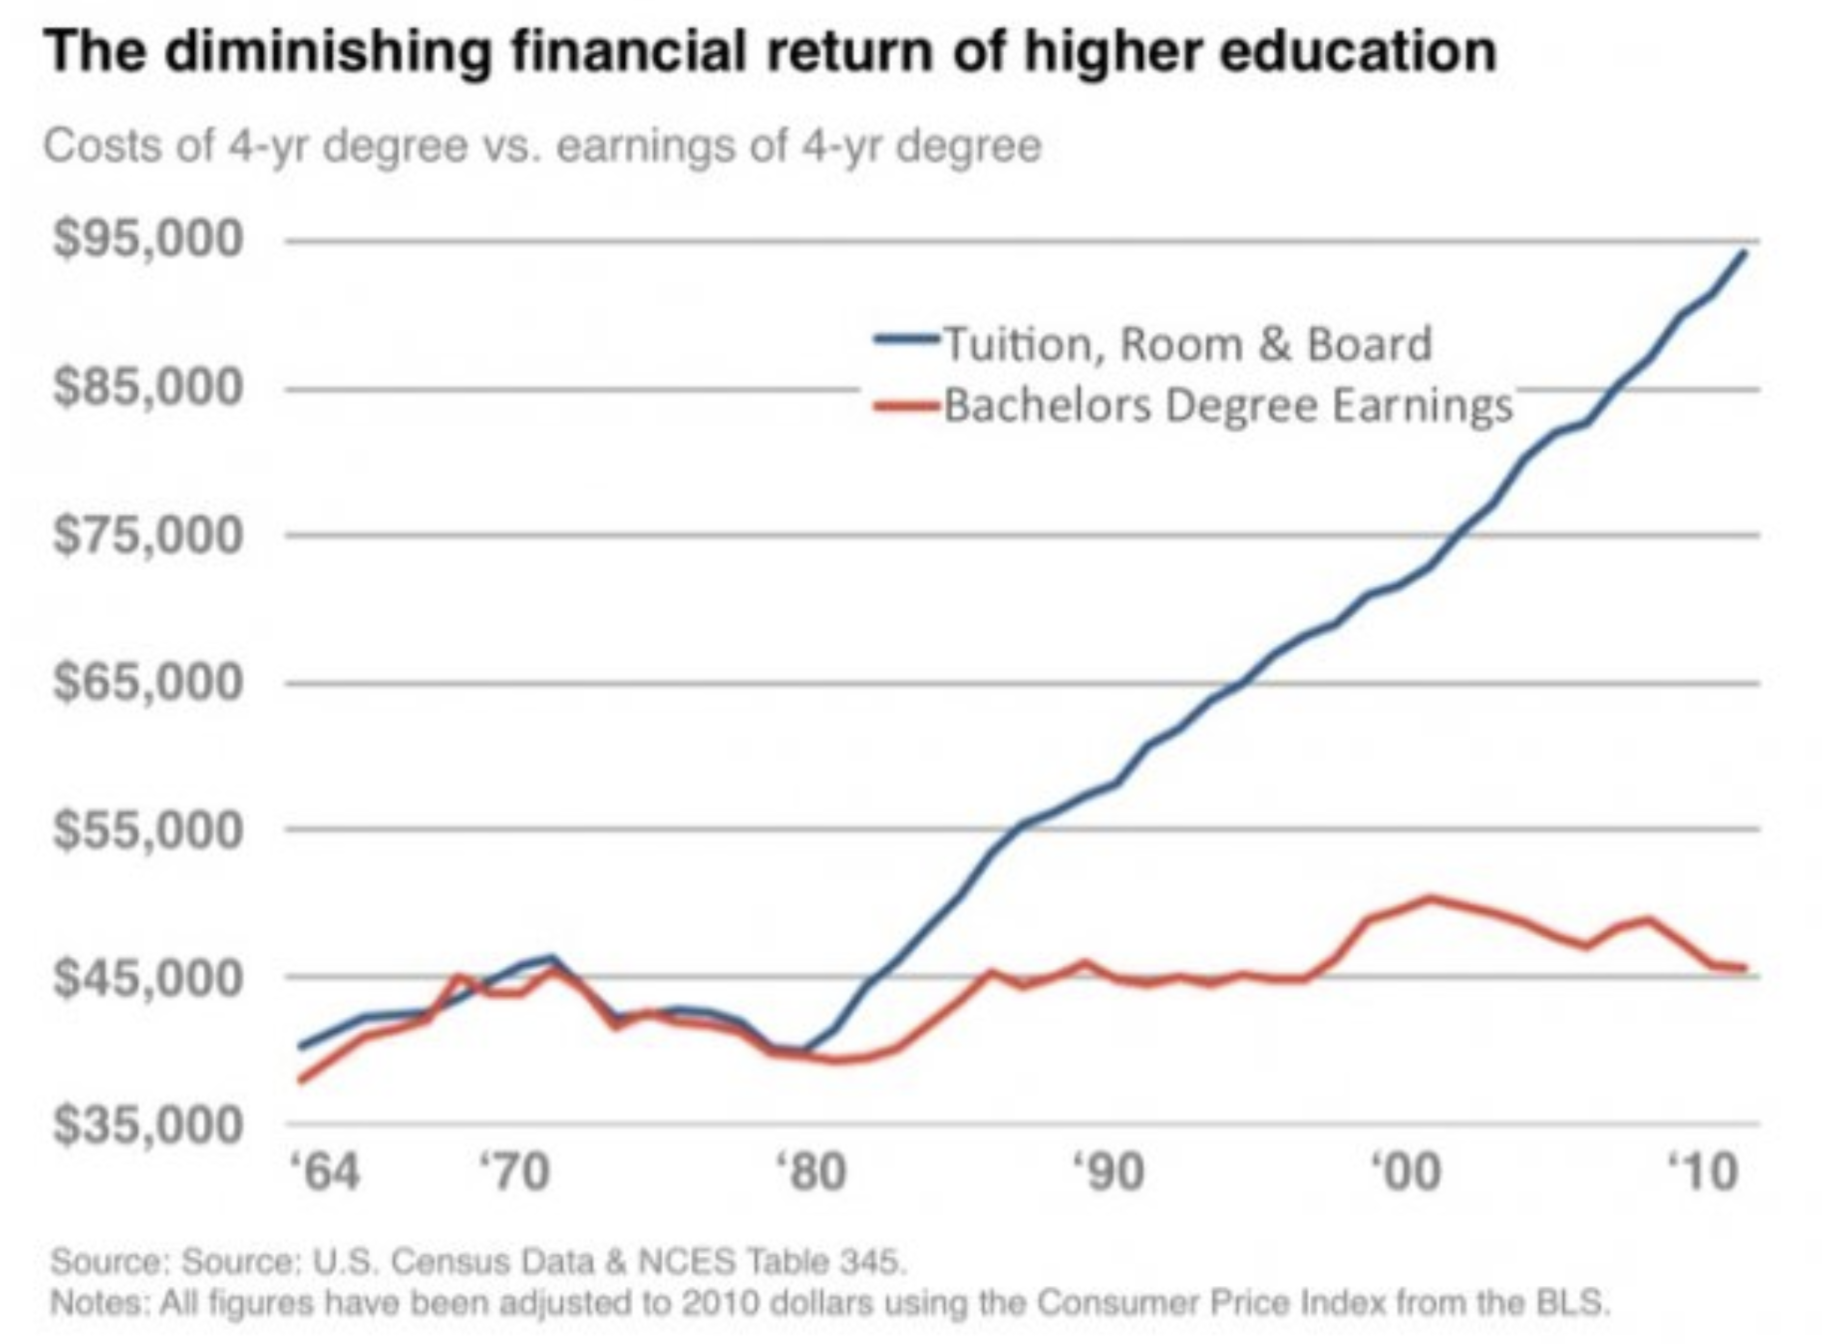
\includegraphics[width=0.7\textwidth,height=\textheight]{img/vis18.png}

~

\begin{itemize}
\item
  \textbf{Good:} All in all, this is a very well made plot. Unnecessary lines and text are kept to a minimum; the title and subtitle are clear. The text size is appropriate. The source of the data is provided.
\item
  \textbf{Bad:} This plot is misleading, because it is plotting data with different units on the same y axis. The blue line is the average \emph{four-year} cost of a college degree. The red line is average \emph{annual} salary for someone with a Bachelor's degree.
\end{itemize}

How should these data be plotted differently in order to correctly explore whether a four-year degree is still worthwhile in terms of its benefits to a 30-year career?

~\\

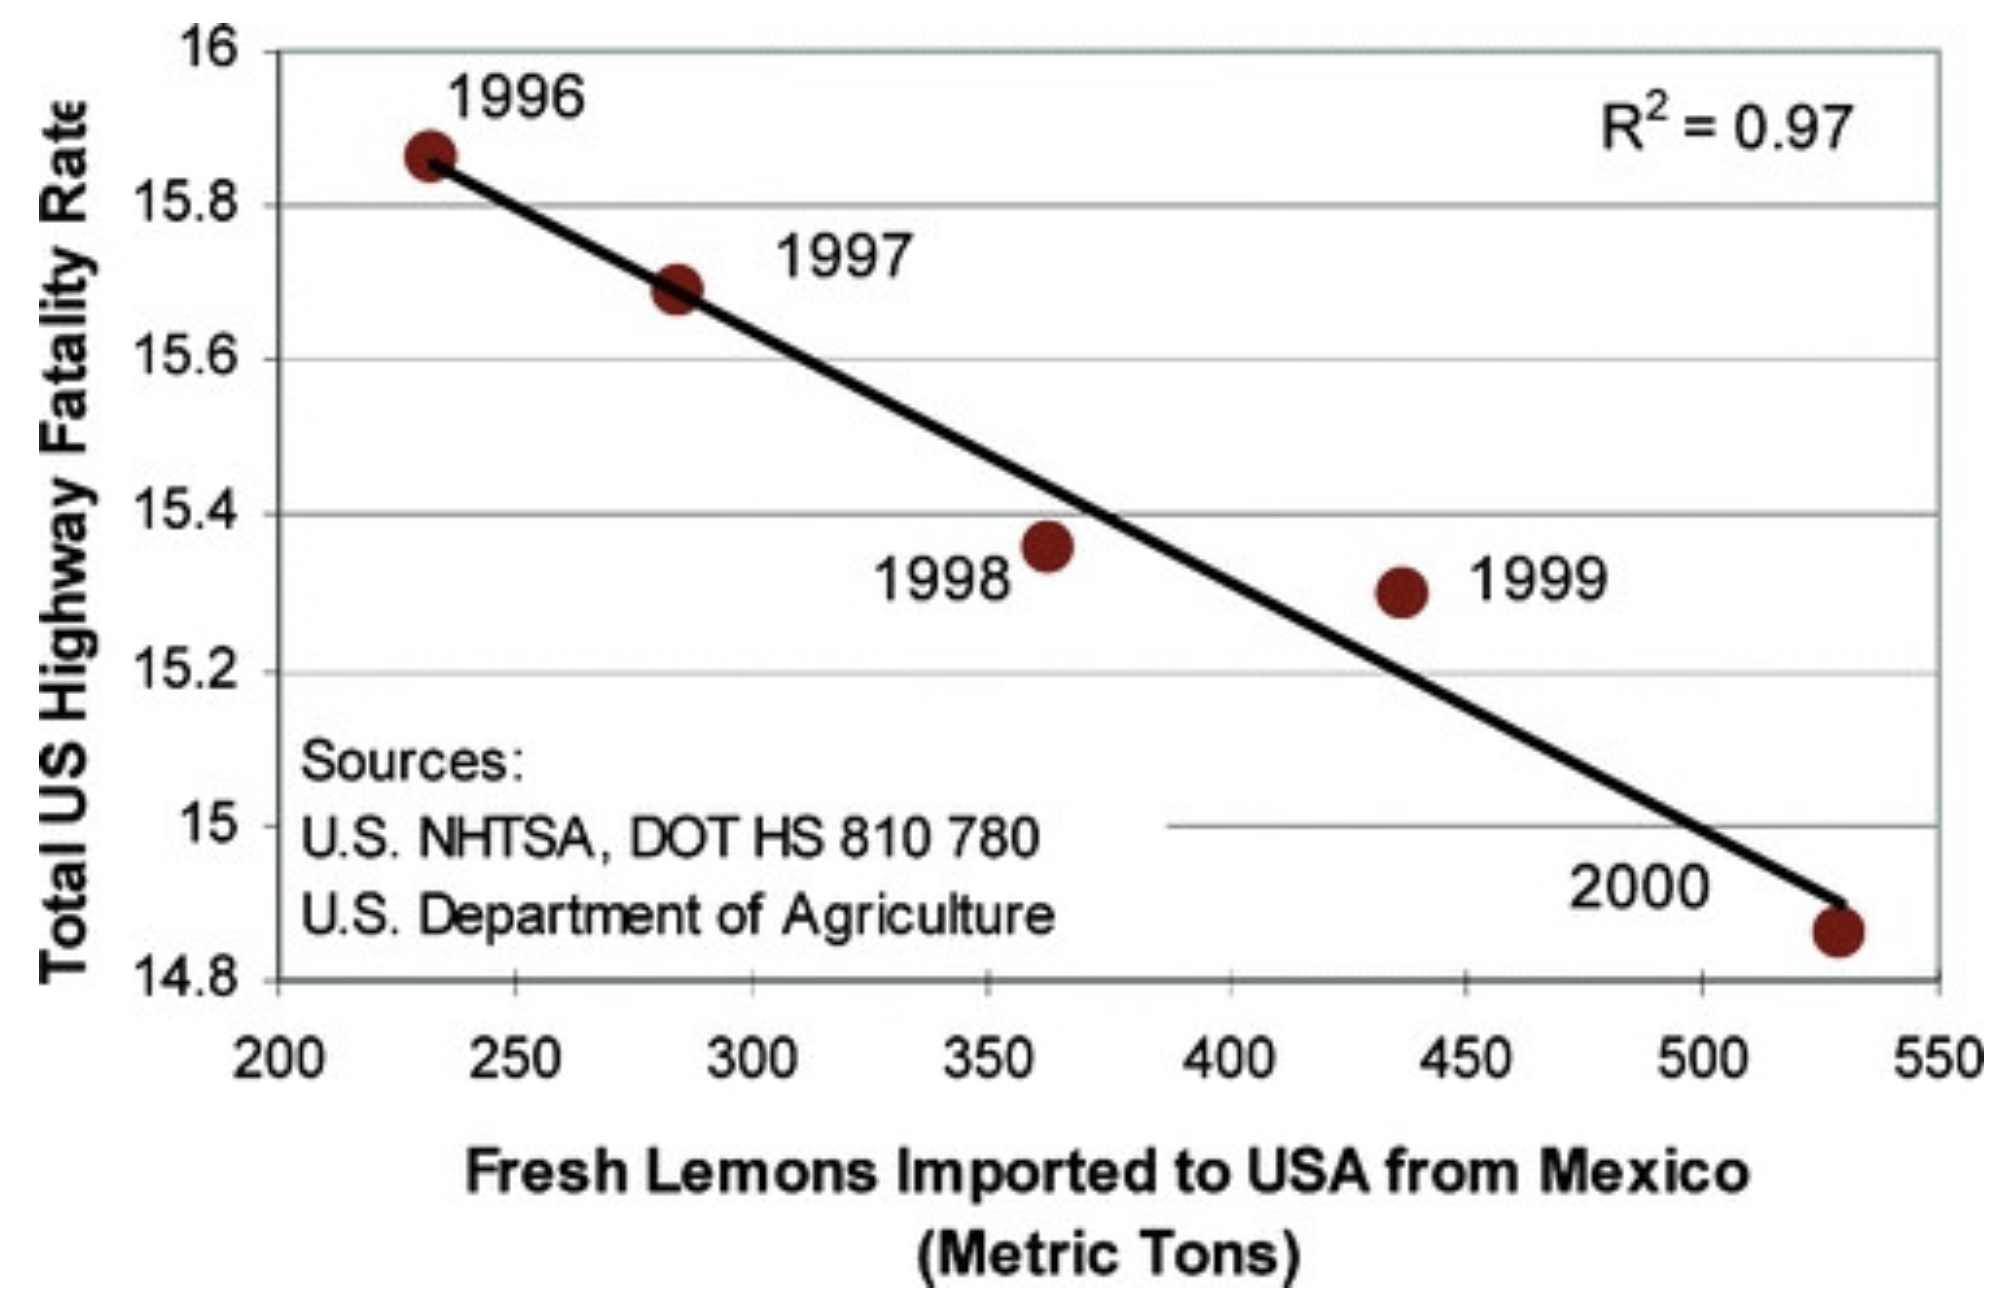
\includegraphics[width=0.7\textwidth,height=\textheight]{img/vis20.png}

~

This is a classic example of a \emph{spurious correlation}: two trends that are correlated but have absolutely nothing to do with each other.

~\\

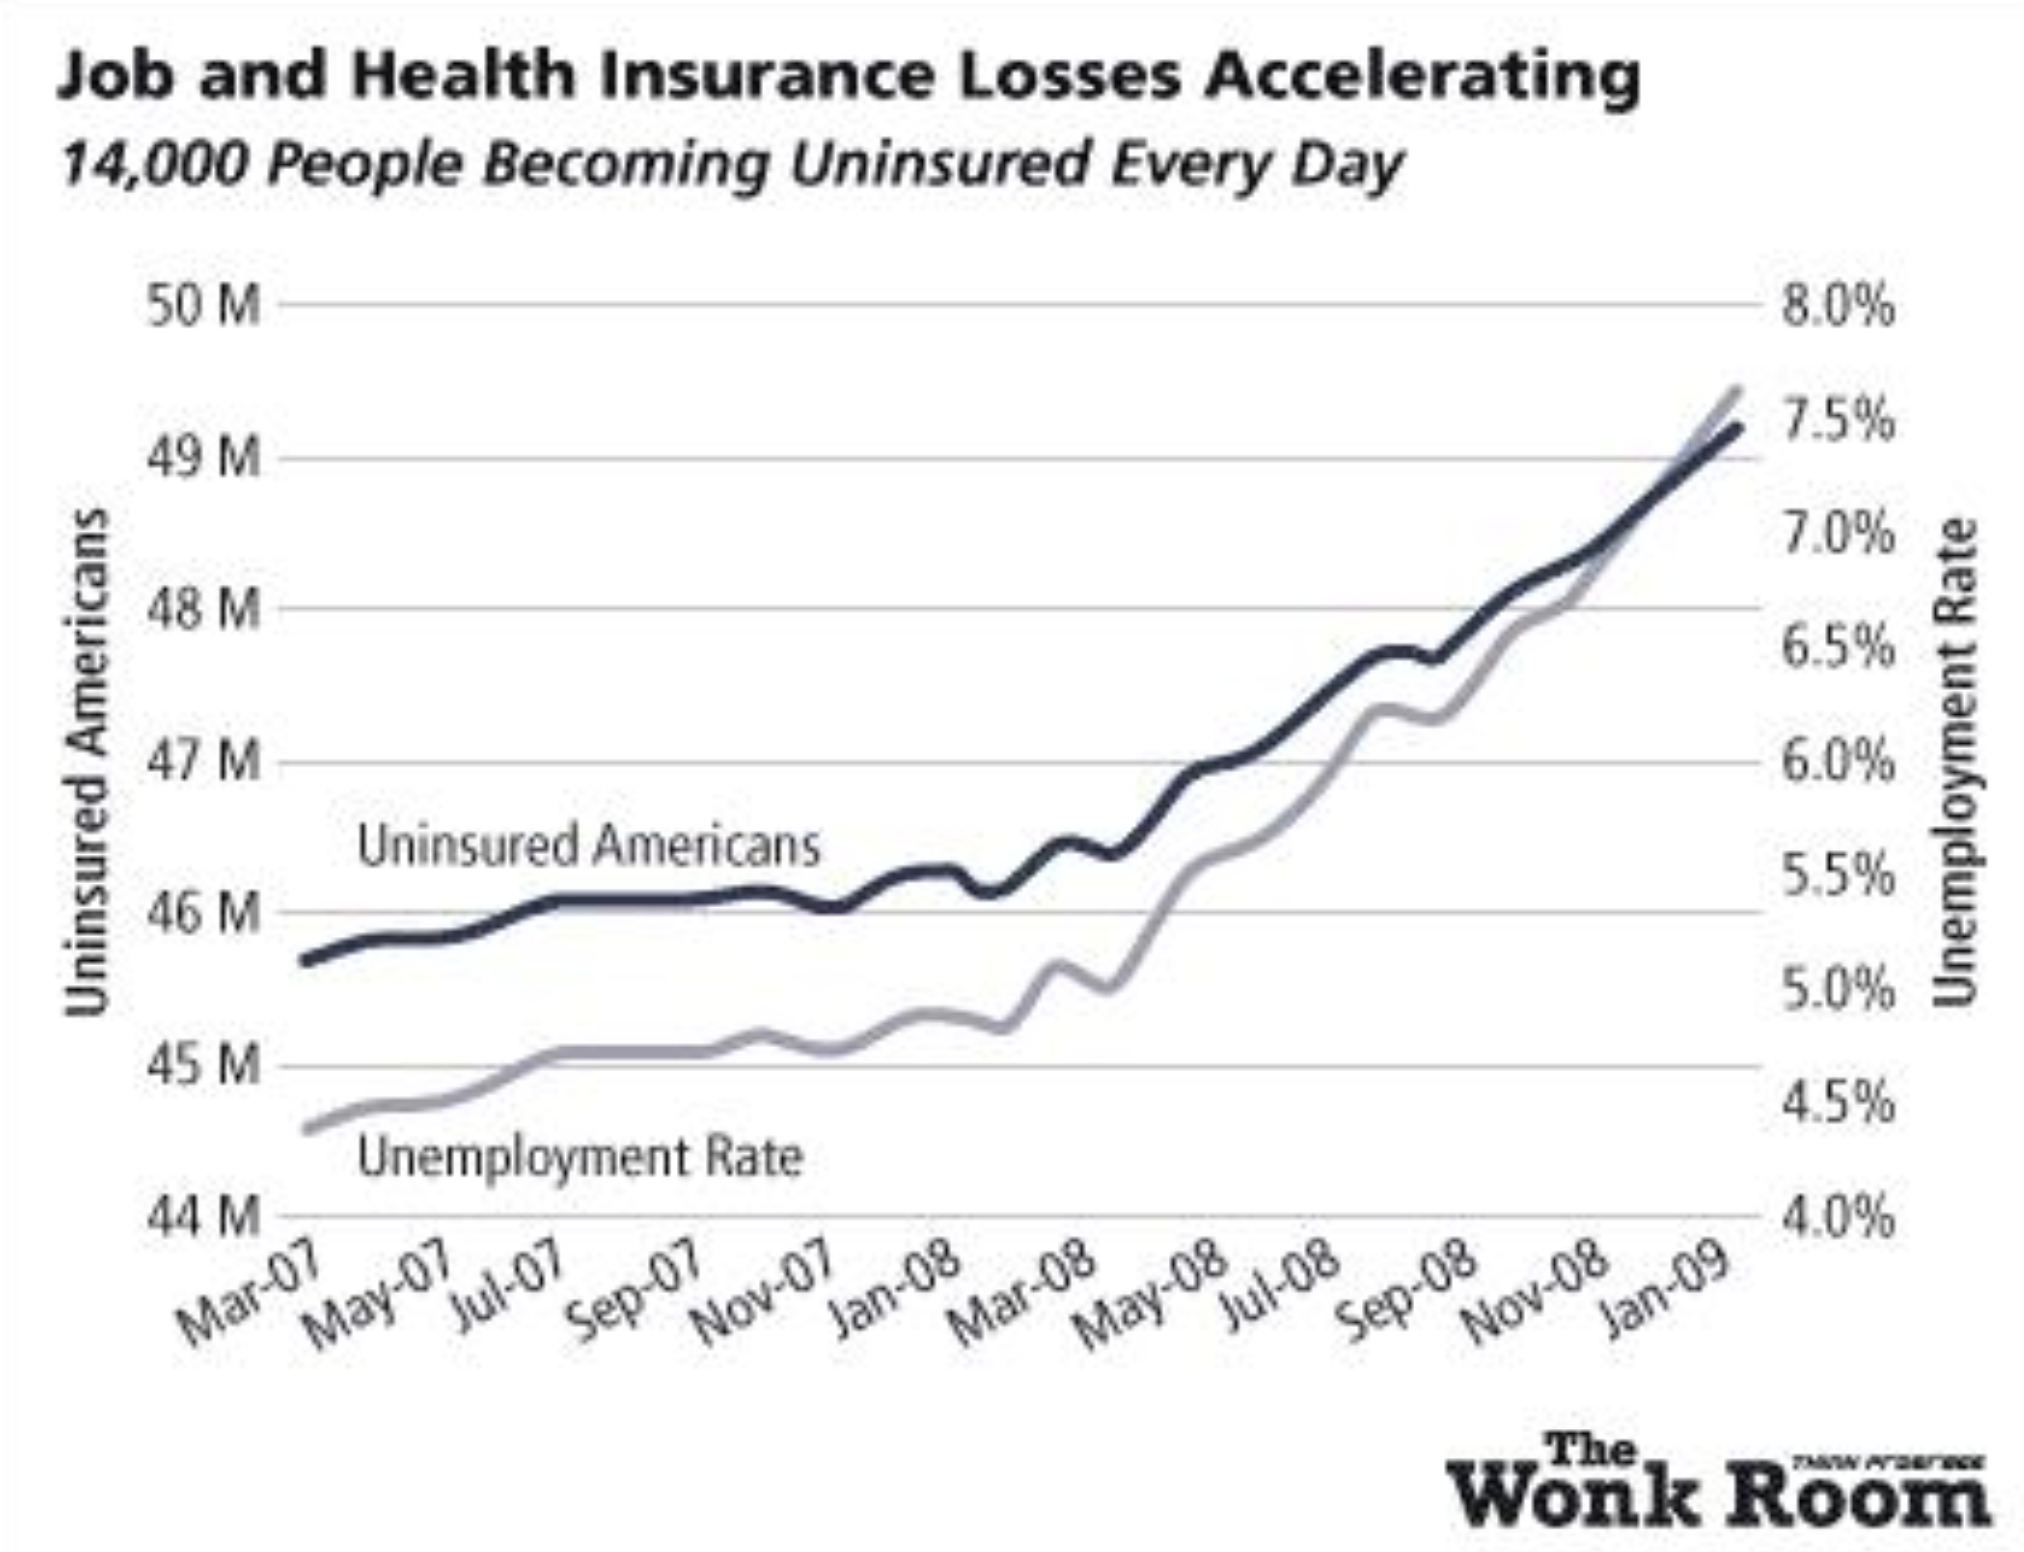
\includegraphics[width=0.7\textwidth,height=\textheight]{img/vis21.png}

~

This is another example of a beautiful plot, but it is also an example of how a plot's message can be coaxed by manipulating y axis scales. If the curve for Uninsured Americans were plotted on the same percentage scale as the Unemployment Rate, it would not seem to be accelerating so rapidly.

~\\

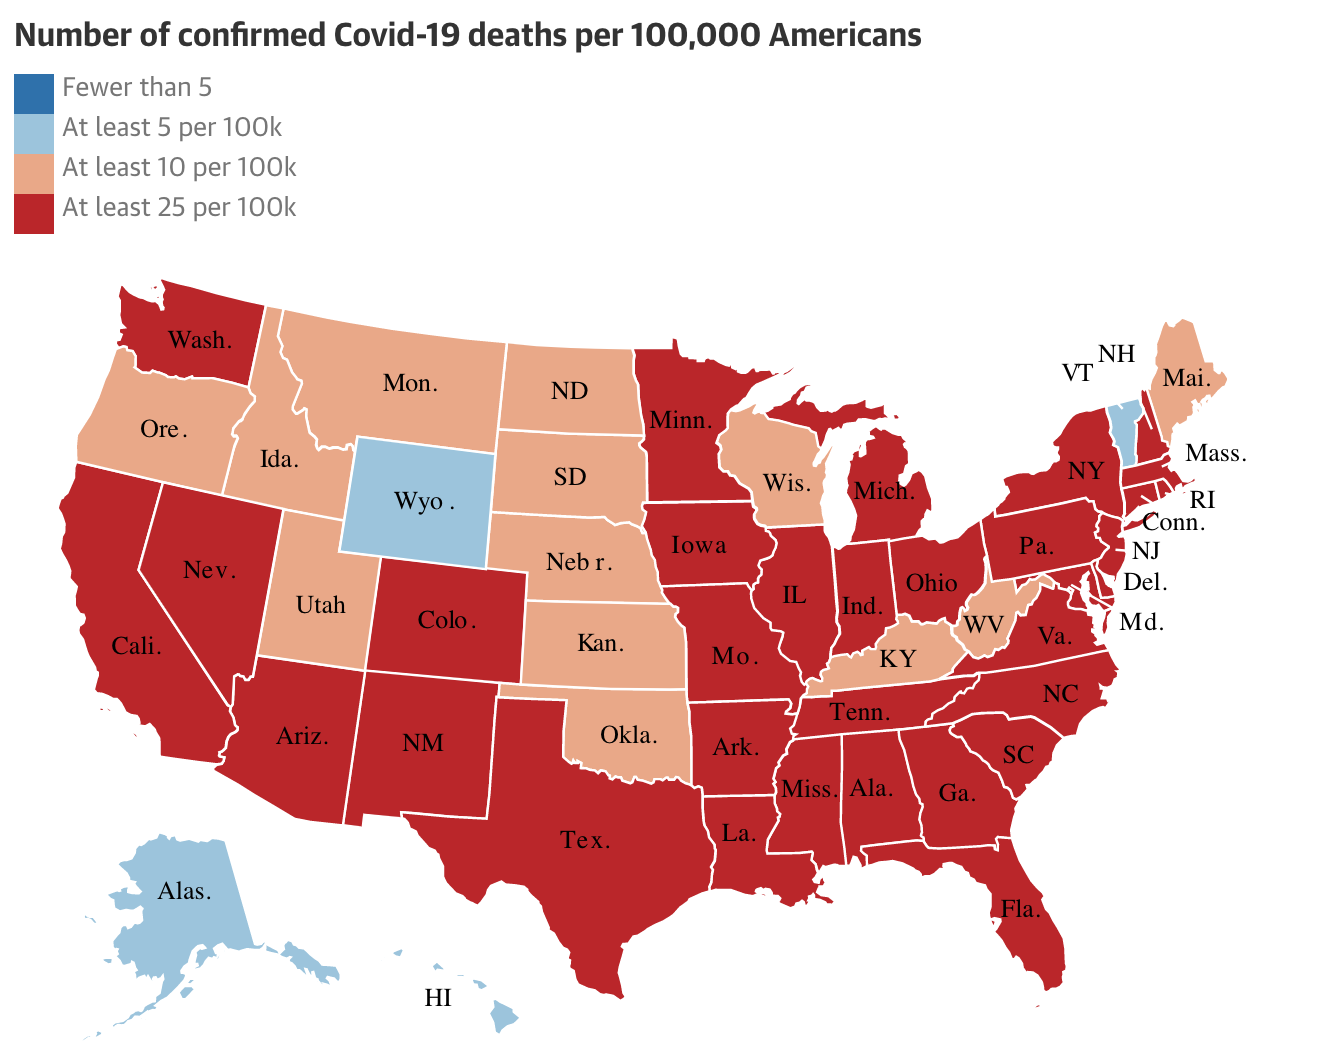
\includegraphics[width=0.9\textwidth,height=\textheight]{img/visb.png}

~

\begin{itemize}
\tightlist
\item
  \textbf{Good:} This is a clean and simple plot, more or less, without too much text.
\item
  \textbf{Good:} The color scale relates to only 4 categories: that is simple enough to make sense of quickly.\\
\item
  \textbf{Good:} The color palette follows an intuitively sequential trend: Blue = low/no bad; Red = high/severe.
\item
  \textbf{Bad:} The abbreviation system for states is inconsistent. Some use initials, some use abbreviations; some use a period, some don't.\\
\item
  \textbf{Bad:} The lowest color category is not used in this plot, and could be removed to increase simplicity.\\
\item
  \textbf{Bad:} Showing a map of the U.S. states with this particular color scale can be confusing: if you had to guess what this chart is about, you would probably assume it is an electoral map.
\end{itemize}

~\\

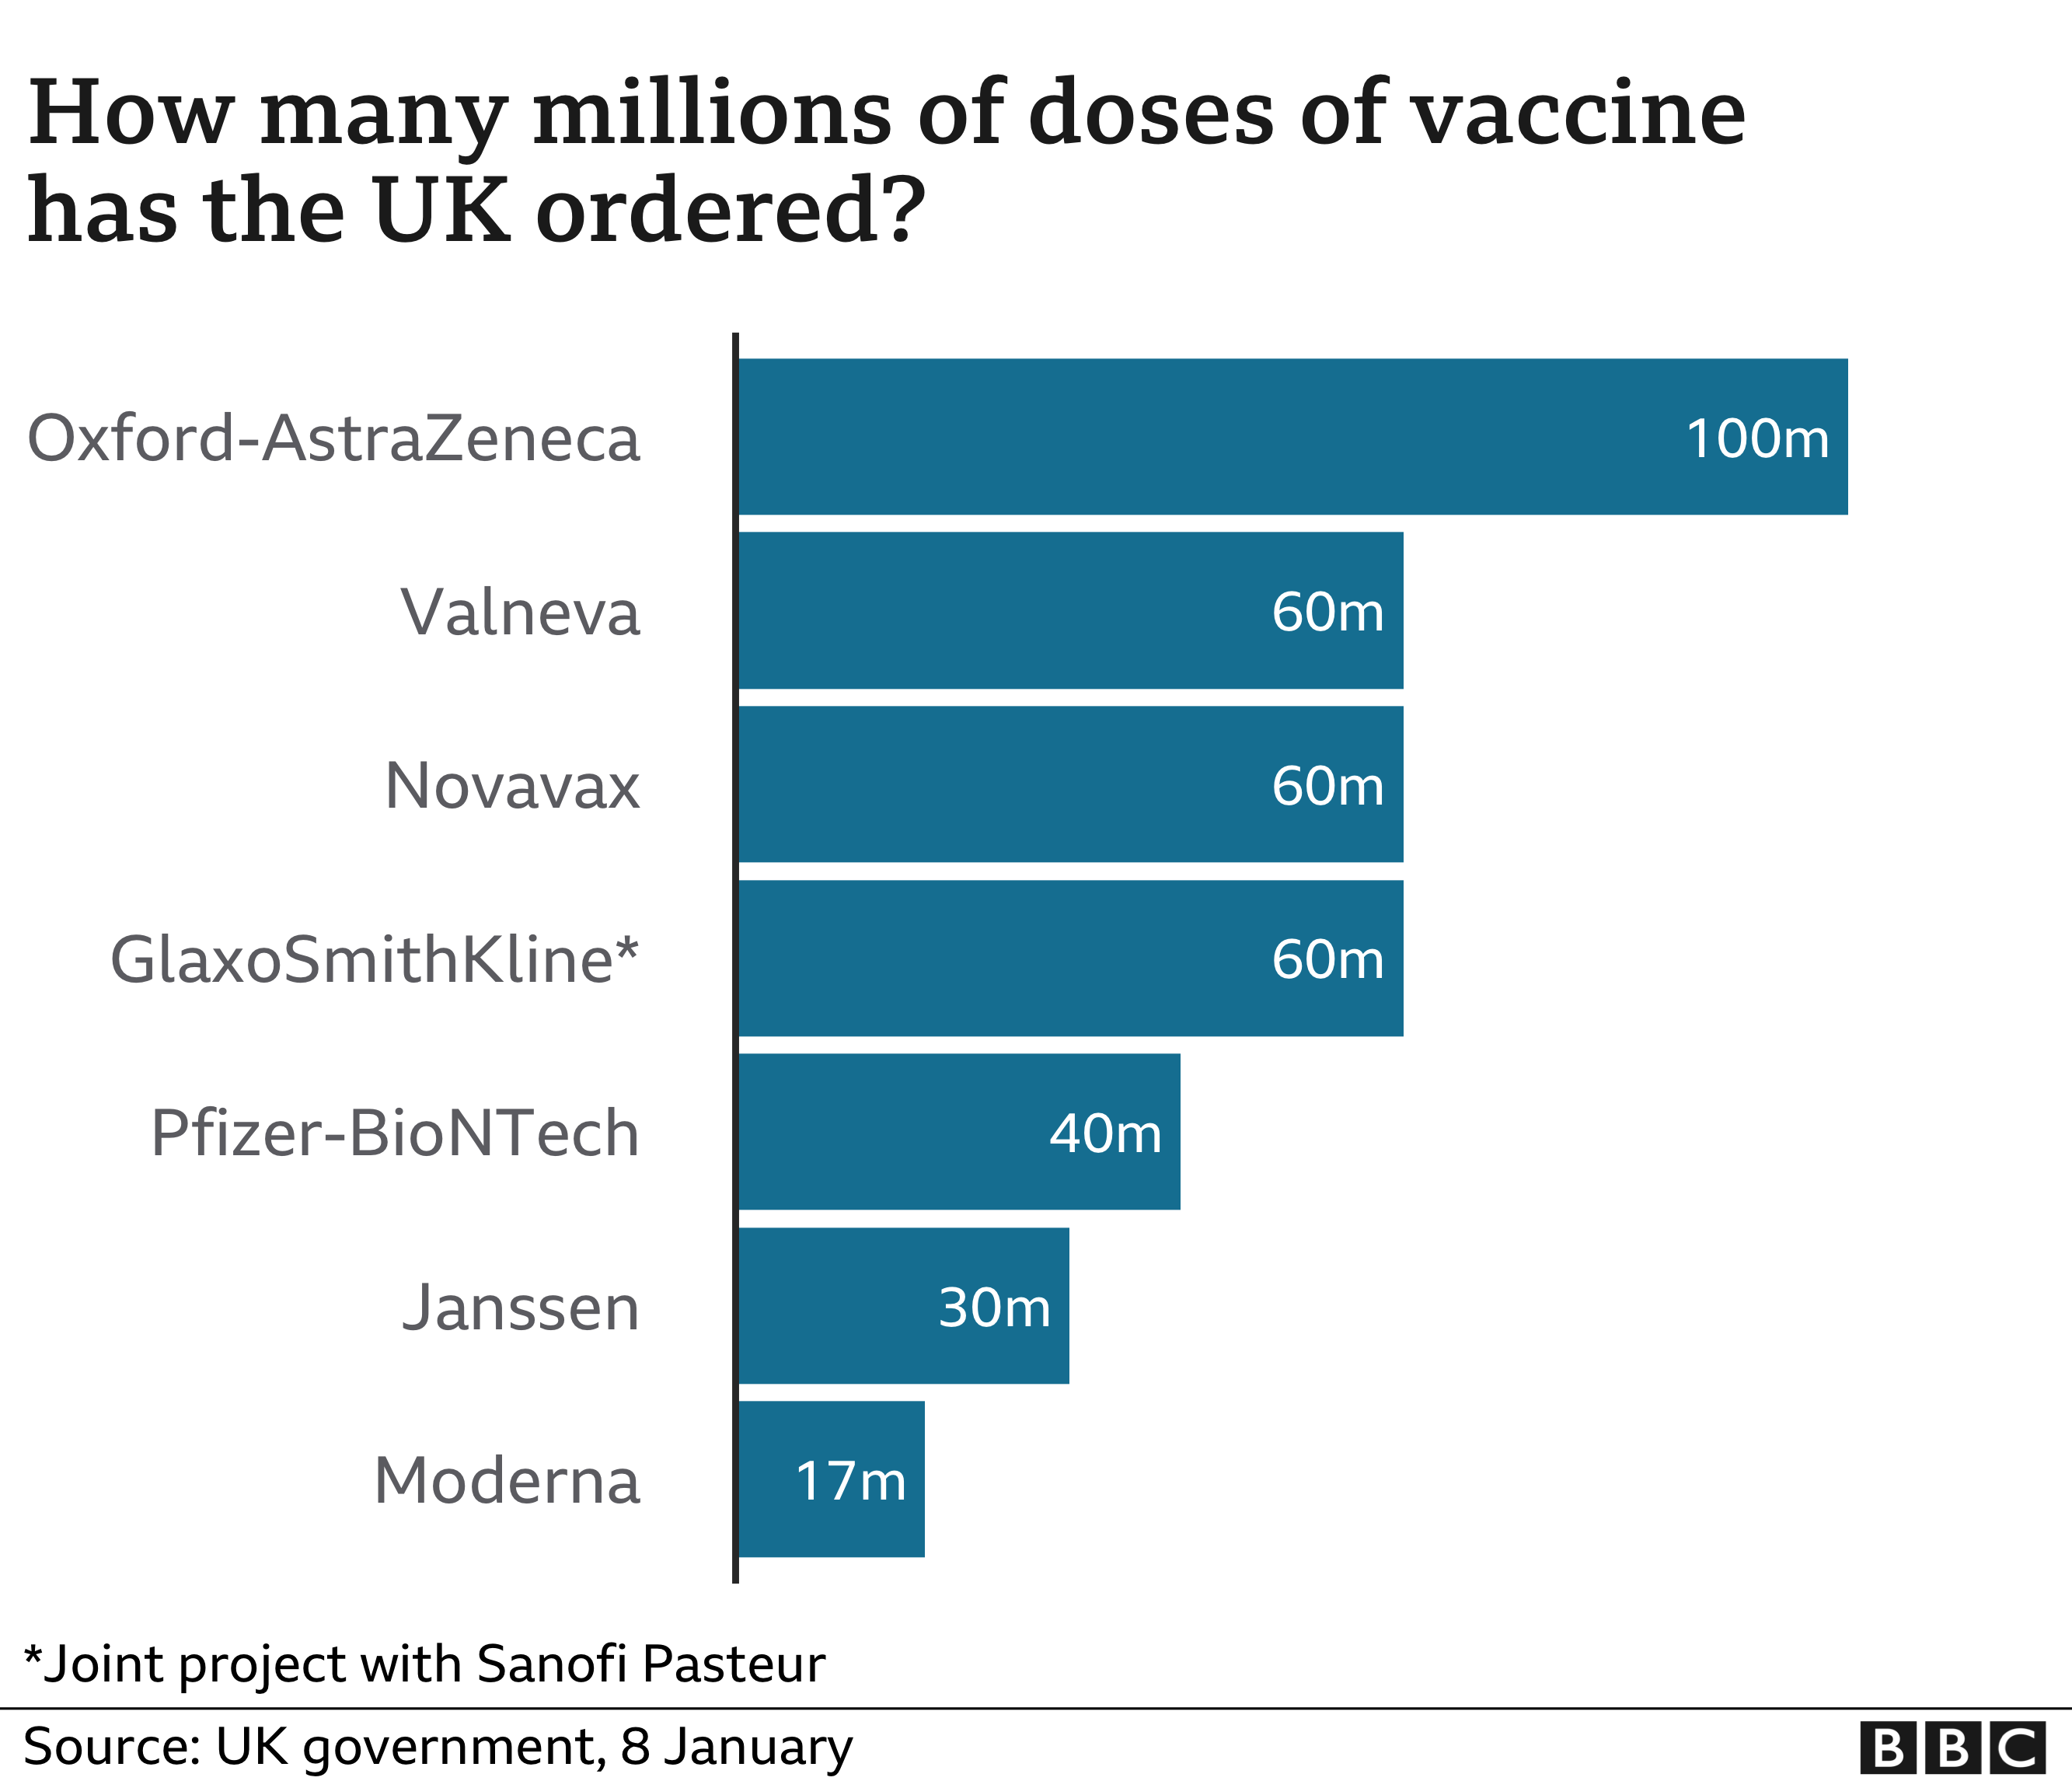
\includegraphics[width=0.75\textwidth,height=\textheight]{img/visc.png}

~

\begin{itemize}
\tightlist
\item
  \textbf{Good:} This is a nice plot. It is simple and junk-free. No unnecessary text or axes.
\item
  \textbf{Good:} Large font, strong color contrast.\\
\item
  \textbf{Good:} The axis starts at zero, and the bars widths are proportional to the data, e.g., the 30m bar is half the width of the 60m bar.\\
\item
  \textbf{Good:} Since this plot is so simple, the actual numbers for each bar can be included without cluttering the plot.
\end{itemize}

~\\
\textbf{Effectiveness of COVID-19 vaccine BNT162b2:}

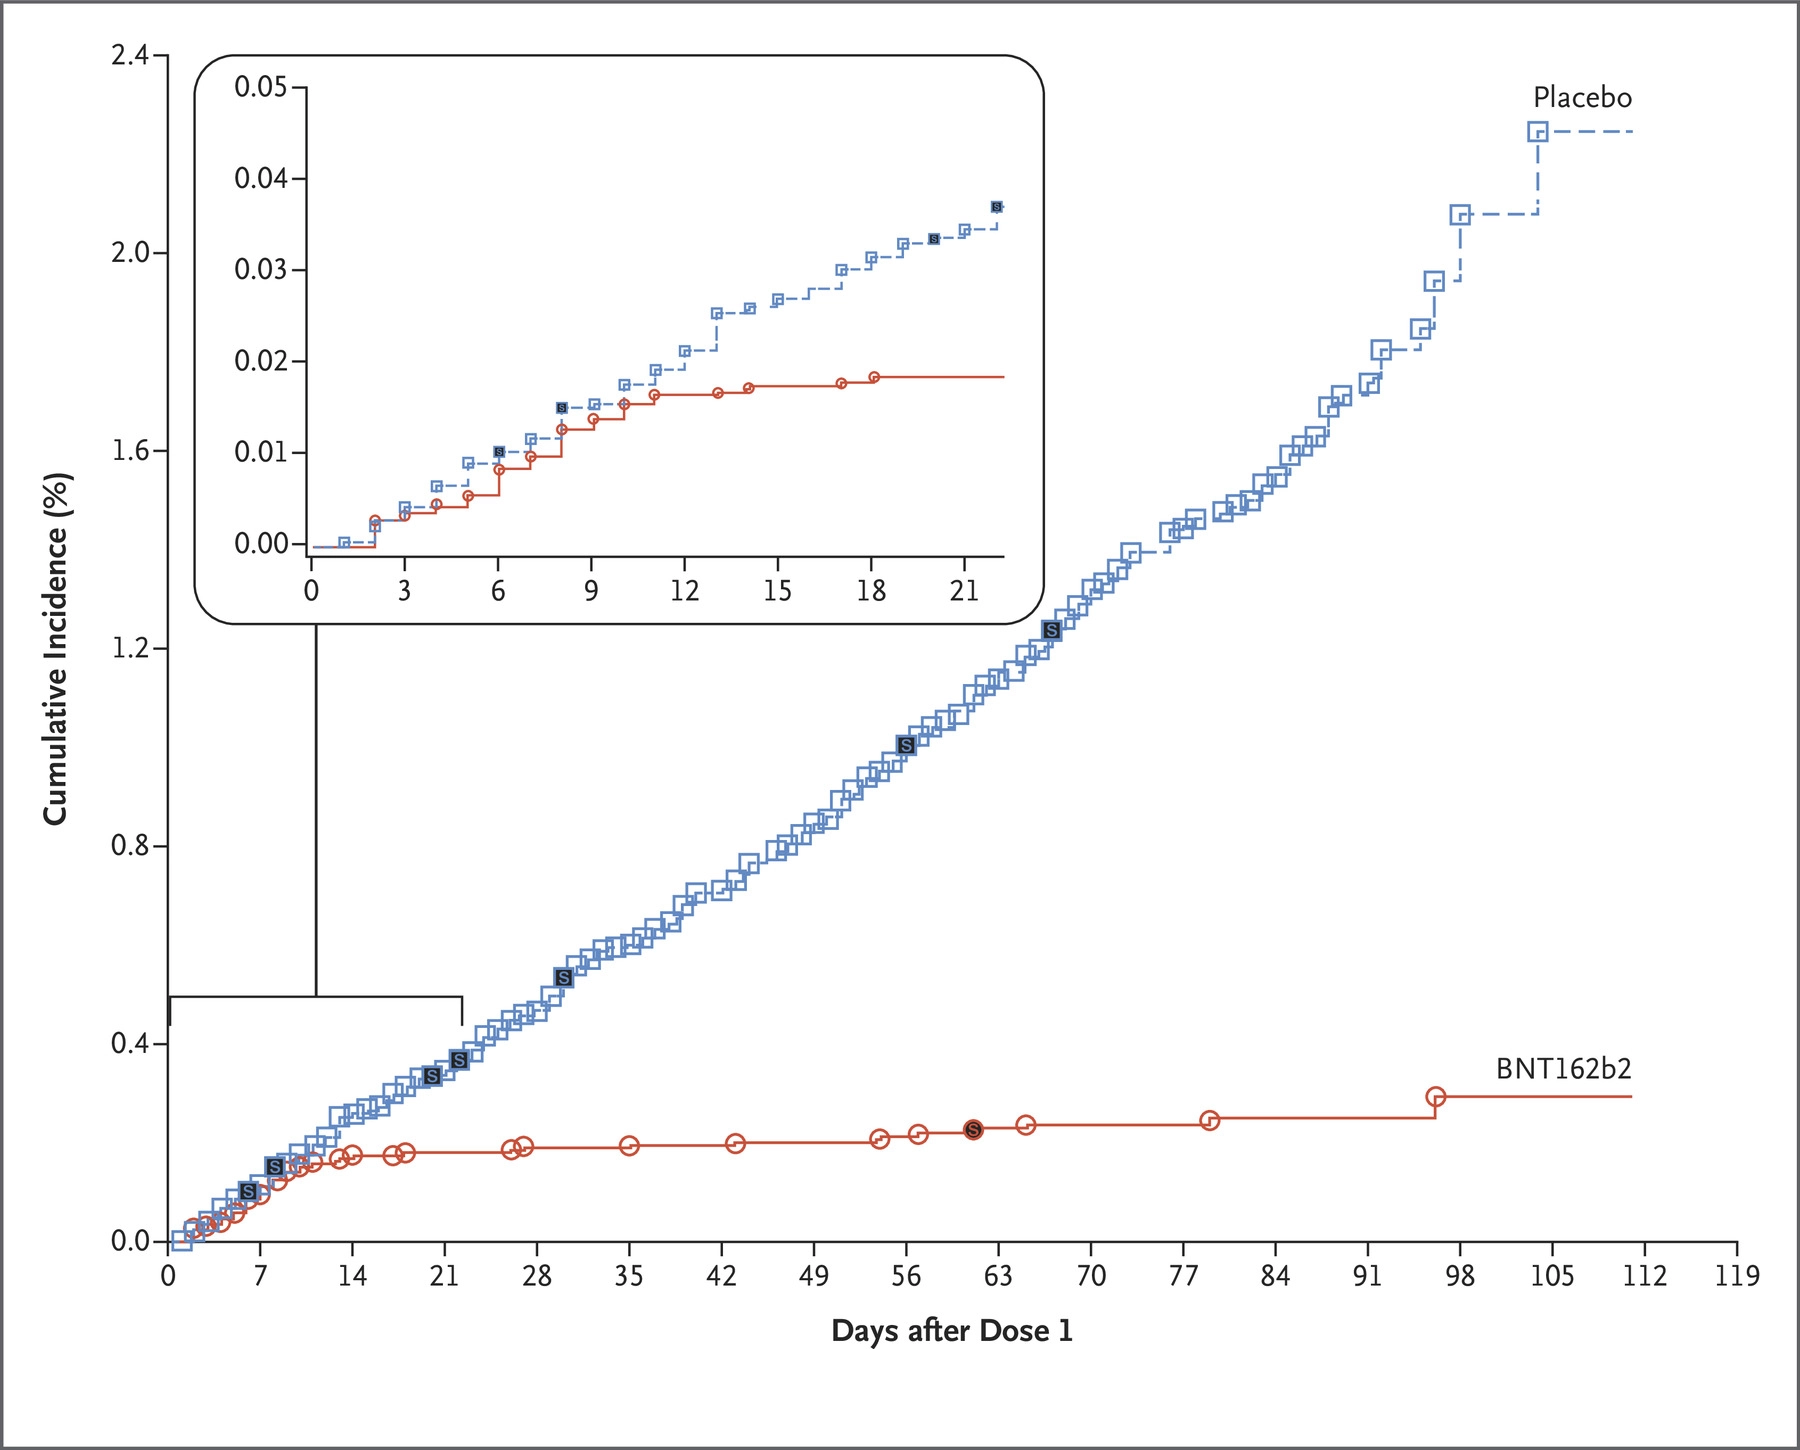
\includegraphics[width=0.8\textwidth,height=\textheight]{img/visd.png}

~

\begin{itemize}
\item
  \textbf{Good:} This is a simple plot that tells a good story: a week or so after receiving a dose, vaccinated participants contracted COVID-19 at a much lower rate than those who received the placebo.
\item
  \textbf{Bad:} The labels are not clear to viewers who are not clinical virologists. To every extent possible, data visualizations should be inclusive and inviting. Don't make someone feel stupid by forcing them to look at their plot.
\item
  \textbf{Bad:} The overlay that zooms in on the first three weeks makes this plot a bit cluttered. We might suggest plotting those first three weeks in a separate plot, adjacent to this one but not embedded within it.
\item
  \textbf{Ugly:} This is an effective plot, but it is not beautiful. What would you do to make this plot more beautiful without compromising its message?
\end{itemize}

~\\

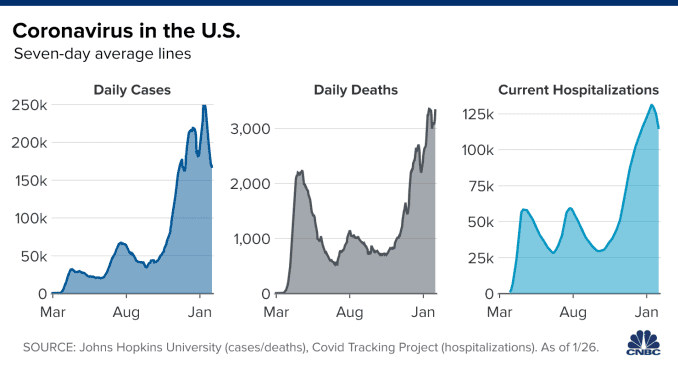
\includegraphics{img/vise.png}

~

\begin{itemize}
\item
  \textbf{Good:} These are clear and simple plots with an obvious take away: daily COVID-19 case counts correspond to deaths and hospitalizations.
\item
  \textbf{Good:} No extraneous labels or lines. These plots are chart-junk free.
\end{itemize}

What do you think about the choice to use three different scales for the y axis? That tends to lead to confusion, but do you think that, in this case, it was justified?

~\\

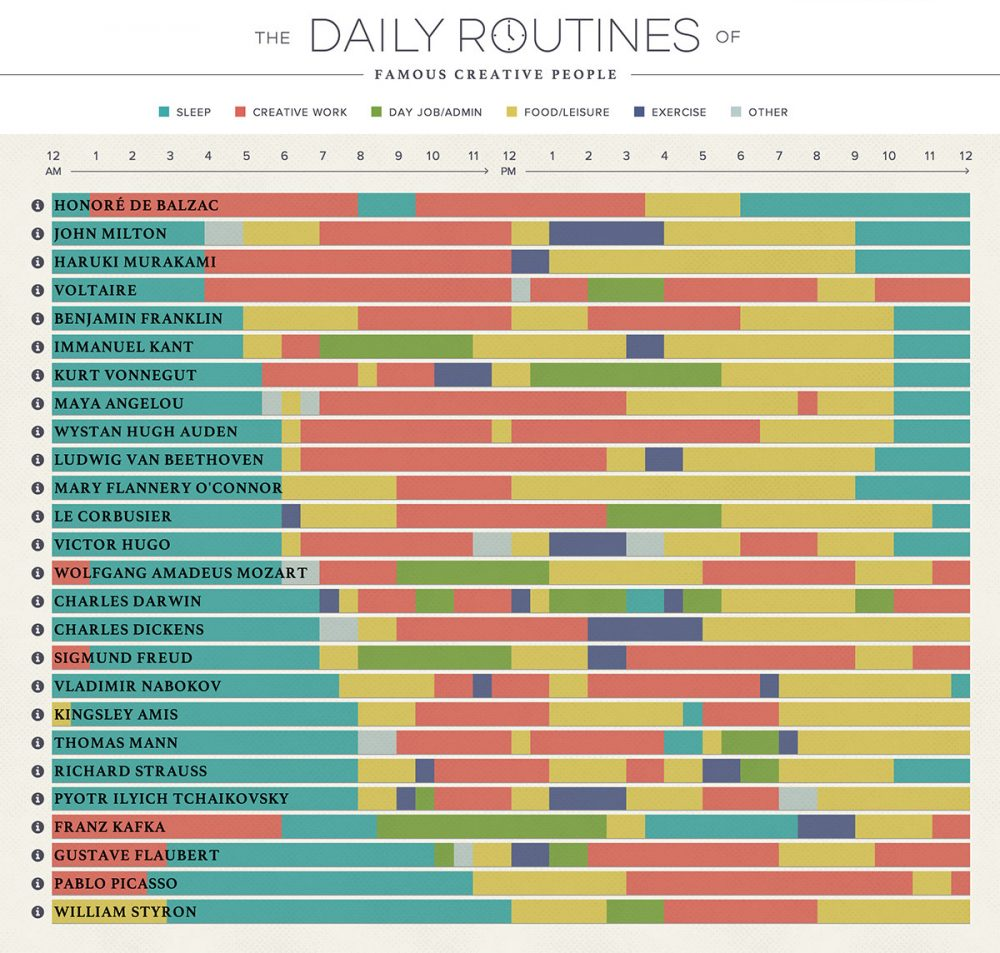
\includegraphics{img/vis-routines.jpeg}

~

Now this is a \href{https://podio.com/site/creative-routines}{data visualization}! It is a tad complicated, but it is elegant and fun to explore.

~\\

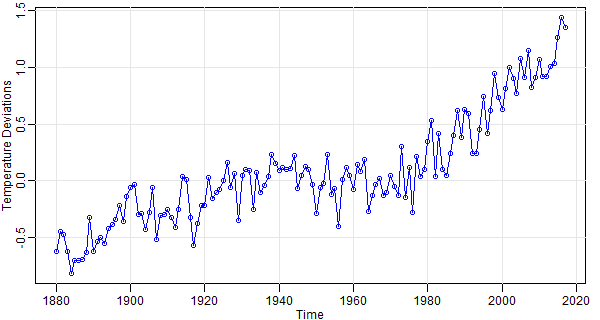
\includegraphics{img/visi.png}

~

This plot is straightforward and simple.

\begin{itemize}
\tightlist
\item
  What it is showing is fairly self-explanatory, though some viewers might benefit from a more informative y-axis label.
\item
  To help explain the y axis, it may be helpful to include a helper line at 0.0 degrees.\\
\item
  Are the points really necessary? Since it is fairly clear that this is an annual dataset, those points are just repeating the information contained in the line, aren't they?
\end{itemize}

~\\

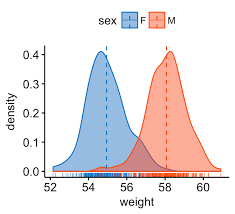
\includegraphics[width=0.5\textwidth,height=\textheight]{img/visf.png}

~

Another straightforward and simple plot, whose meaning is pretty obvious even without a title.

\begin{itemize}
\tightlist
\item
  Some more effort could have gone into the x axis label. Are the units kilograms, or pounds?
\item
  This plot conveys a lot of information really intuitively. You can intuit that the dotted lines are probably mean weights; that the distributions show the range of data.\\
\item
  The semi-transparent colors make it possible to see how the two distributions overlap. Very helpful!
\item
  It is interesting that the male/female color associations are opposite the convention. Do you think that was intentional?\\
\item
  Note the little tick marks along the x axis. That is a suble way of indicating sample size; it shows how much data are used to populate each distribution.
\end{itemize}

~\\

\textbf{Some baby names throughout the last 140 years}
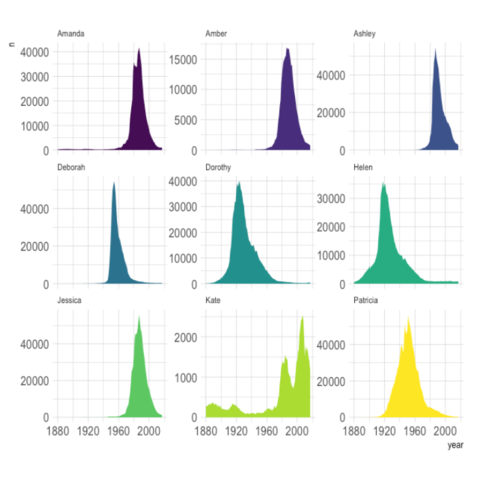
\includegraphics[width=0.7\textwidth,height=\textheight]{img/visg.png}

~

\begin{itemize}
\item
  In this plot, chart junk is kept to a minimum, which is nice, but the names are a little too small to read. It is strange that the names are a smaller font size than the axes labels.
\item
  What do you think about the use of color? The colors are pretty, but it is a purely aesthetic choice; the colors don't correspond to anything about the data at all.
\item
  It was an interesting decision to only include x axis labels on the bottom row of plots. In a way this is nice because it (1) reinforces the fact that each plot is using the same x axis range, and (2) removes redundant content from the plot. However, it makes it a bit more laborious to explore the plots in the top row.
\item
  It was also an interesting decision to make the y axis ranges different for each plot. There are trade-offs to this decision. What would be lost if all of these facets were forced to use the same y axis range?
\end{itemize}

\hypertarget{chart-junk}{%
\section*{Chart junk}\label{chart-junk}}
\addcontentsline{toc}{section}{Chart junk}

A few times already, we have referred to the concept of chart junk. This refers to the idea that the best plots are the ones that minimize the ink-to-data ratio. In other words, there should be no extraneous or unnecessary ink on your plot.

The chart junk principle applies to both graphical and tabular representations of data. Which of these tables is easier to read?

~\\

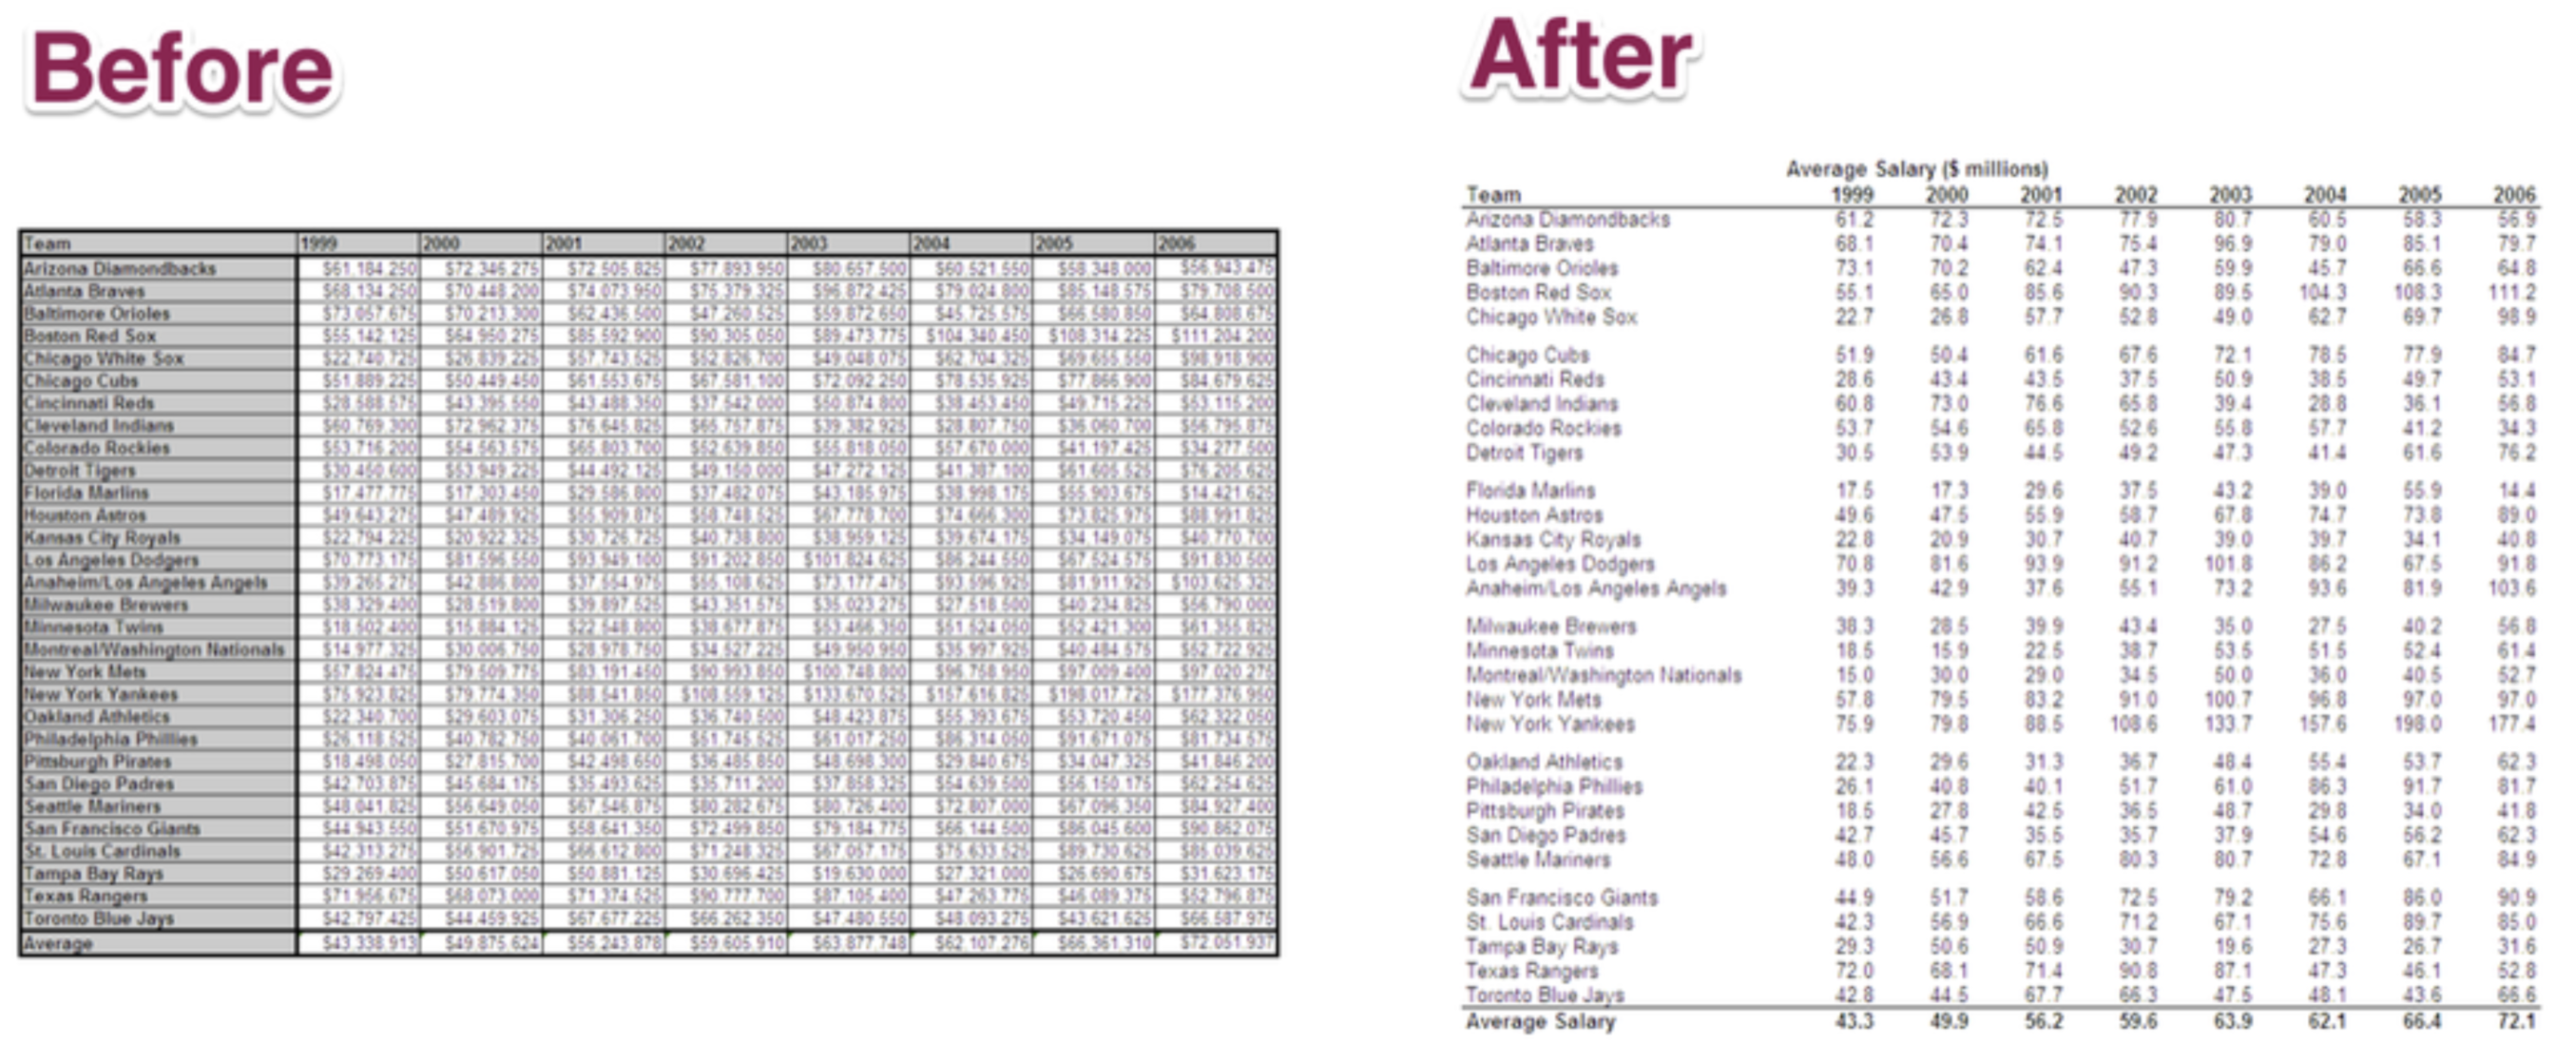
\includegraphics{img/vis17.png}

~

Which of these diagrams is easier to read?

~\\

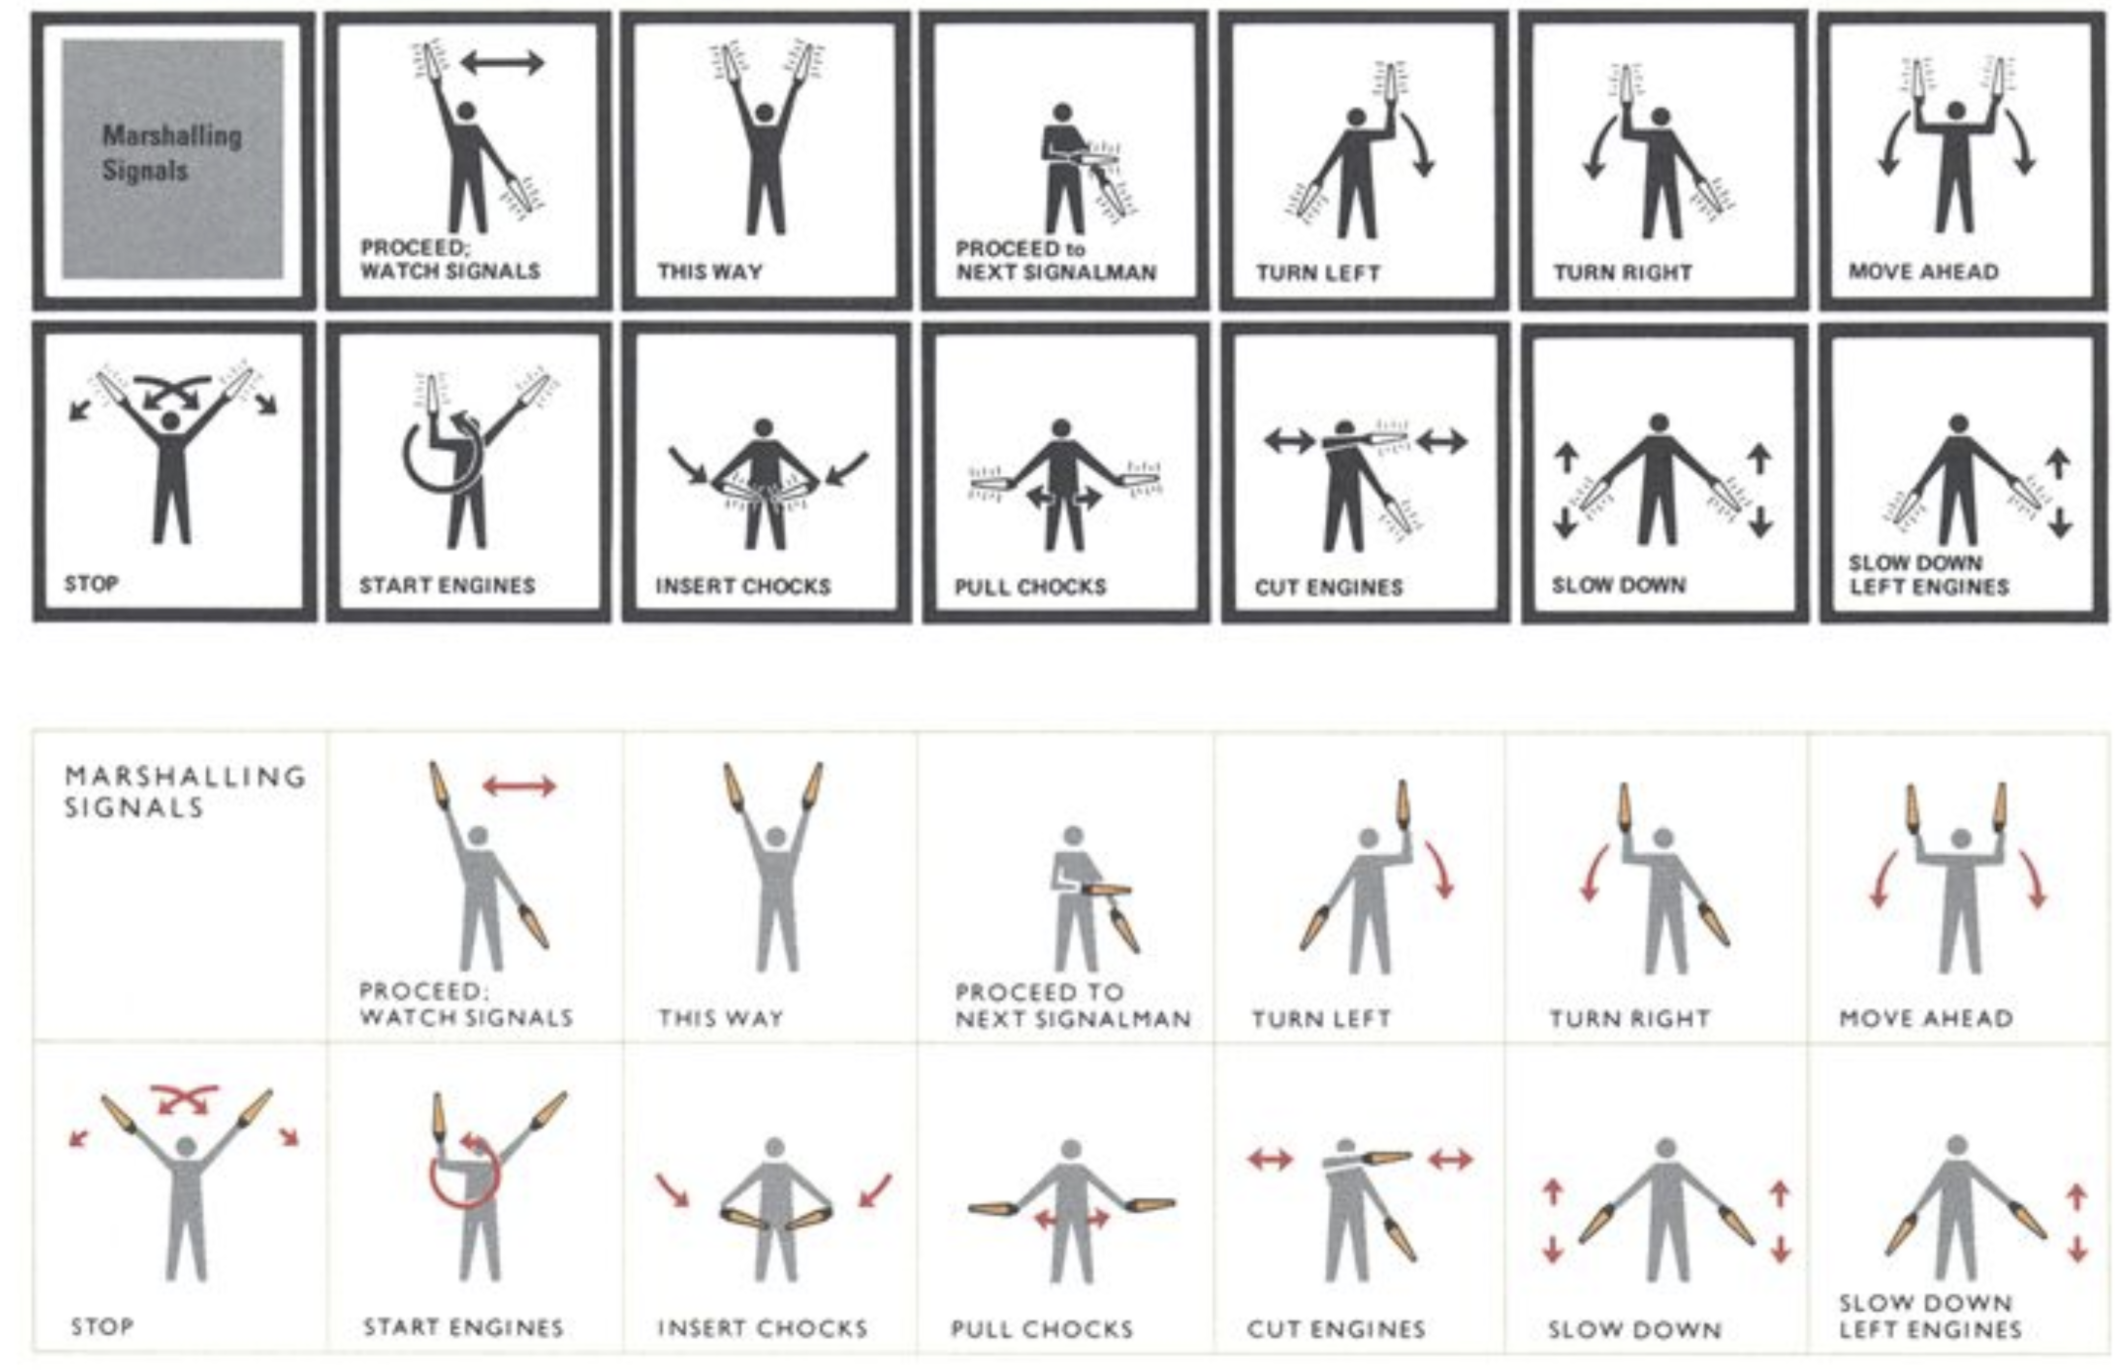
\includegraphics{img/vis19.png}

~

And what about these basic scatterplots? Which is more effective and elegant?

~\\

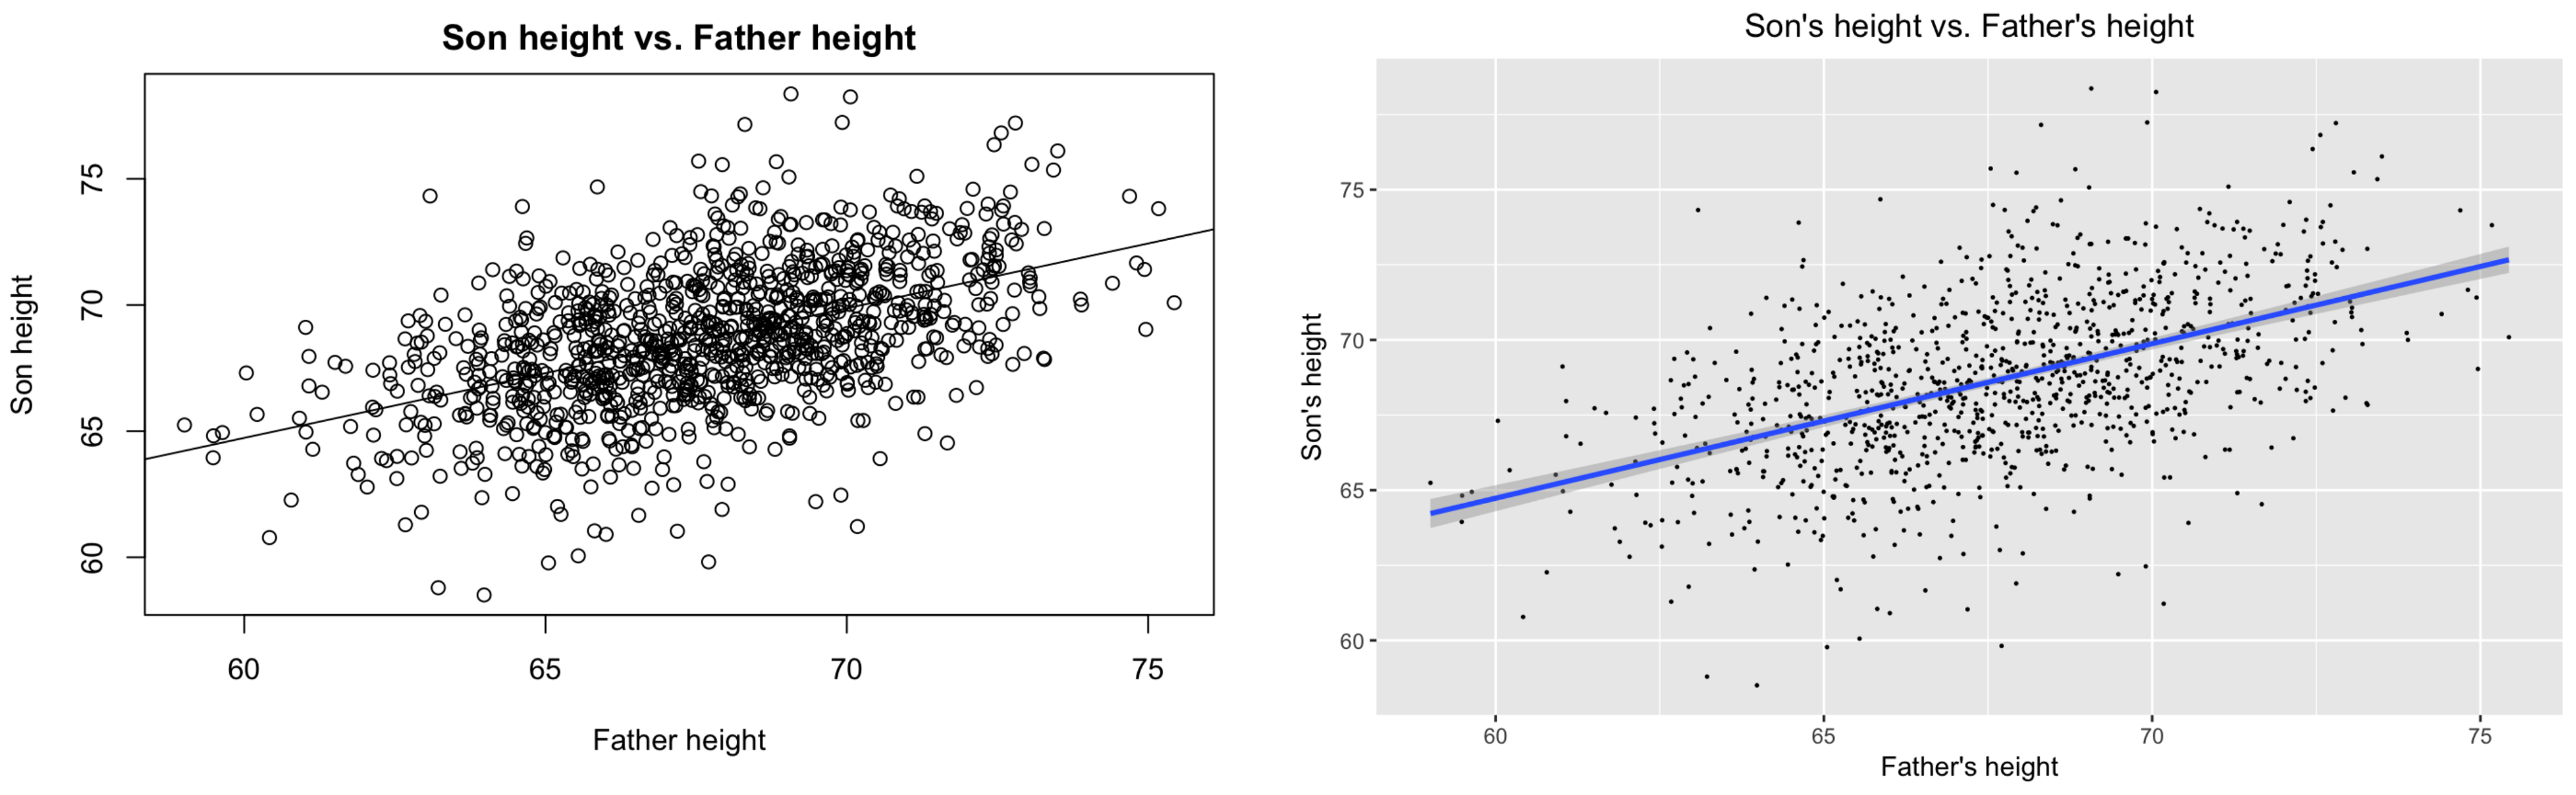
\includegraphics{img/vish.png}

\hypertarget{final-thoughts}{%
\section*{Final thoughts}\label{final-thoughts}}
\addcontentsline{toc}{section}{Final thoughts}

To get a sense of what can be done with data visualization -- and just how enthusiastic data scientists can get about data viz -- enjoy this video by the Swedish epidemiologist \textbf{Hans Rosling,} the pioneer of \textbf{interactive data visualization} (link \href{https://www.youtube.com/watch?v=jbkSRLYSojo\&t=2s}{here}).

~

~

As you go down the rabbit hole of data visualization, it will be important to become familiar with the work of \textbf{Edward Tufte}, the grandfather of thinking about data viz as an art form. This video showcases Tufte and other data scientists who have been inspired by his work (link \href{https://www.youtube.com/watch?v=AdSZJzb-aX8}{here}).

~

~

Finally, this video offers a nice and concise summary of Edward Tufte's principles of data visualization (link \href{https://www.youtube.com/watch?v=r7YdcZkS_1k}{here}).

~

~\\
\hspace*{0.333em}

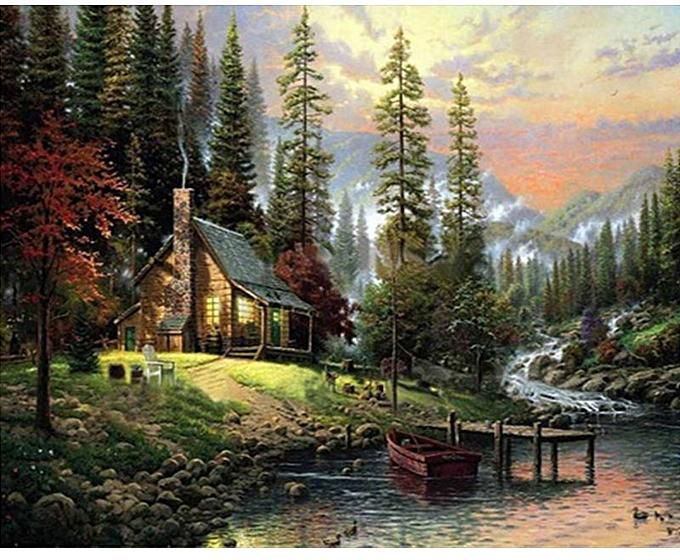
\includegraphics{img/vis-painting.jpeg}

Click here to return to the previous point in the module.

\hypertarget{part-getting-started}{%
\chapter*{\texorpdfstring{(PART) Getting sta\texttt{r}ted}{(PART) Getting started}}\label{part-getting-started}}

\hypertarget{setting-up-rstudio}{%
\chapter{\texorpdfstring{Setting up \texttt{RStudio}}{Setting up RStudio}}\label{setting-up-rstudio}}

First, let's get the right programs installed on your computer. Then we will explain what they are and why you need them.

\textbf{First, download and install \texttt{R}: }

Go to the following website, click the \emph{Download} button, and follow the website's instructions from there.
\url{https://mirrors.nics.utk.edu/cran/}

\textbf{Second, download and install \texttt{RStudio}:}

Go to the following website and choose the free Desktop version:
\url{https://rstudio.com/products/rstudio/download/}

\textbf{Third, make sure \texttt{RStudio} opens successfully:}

Open the \texttt{RStudio} app. A window should appear that looks like this:

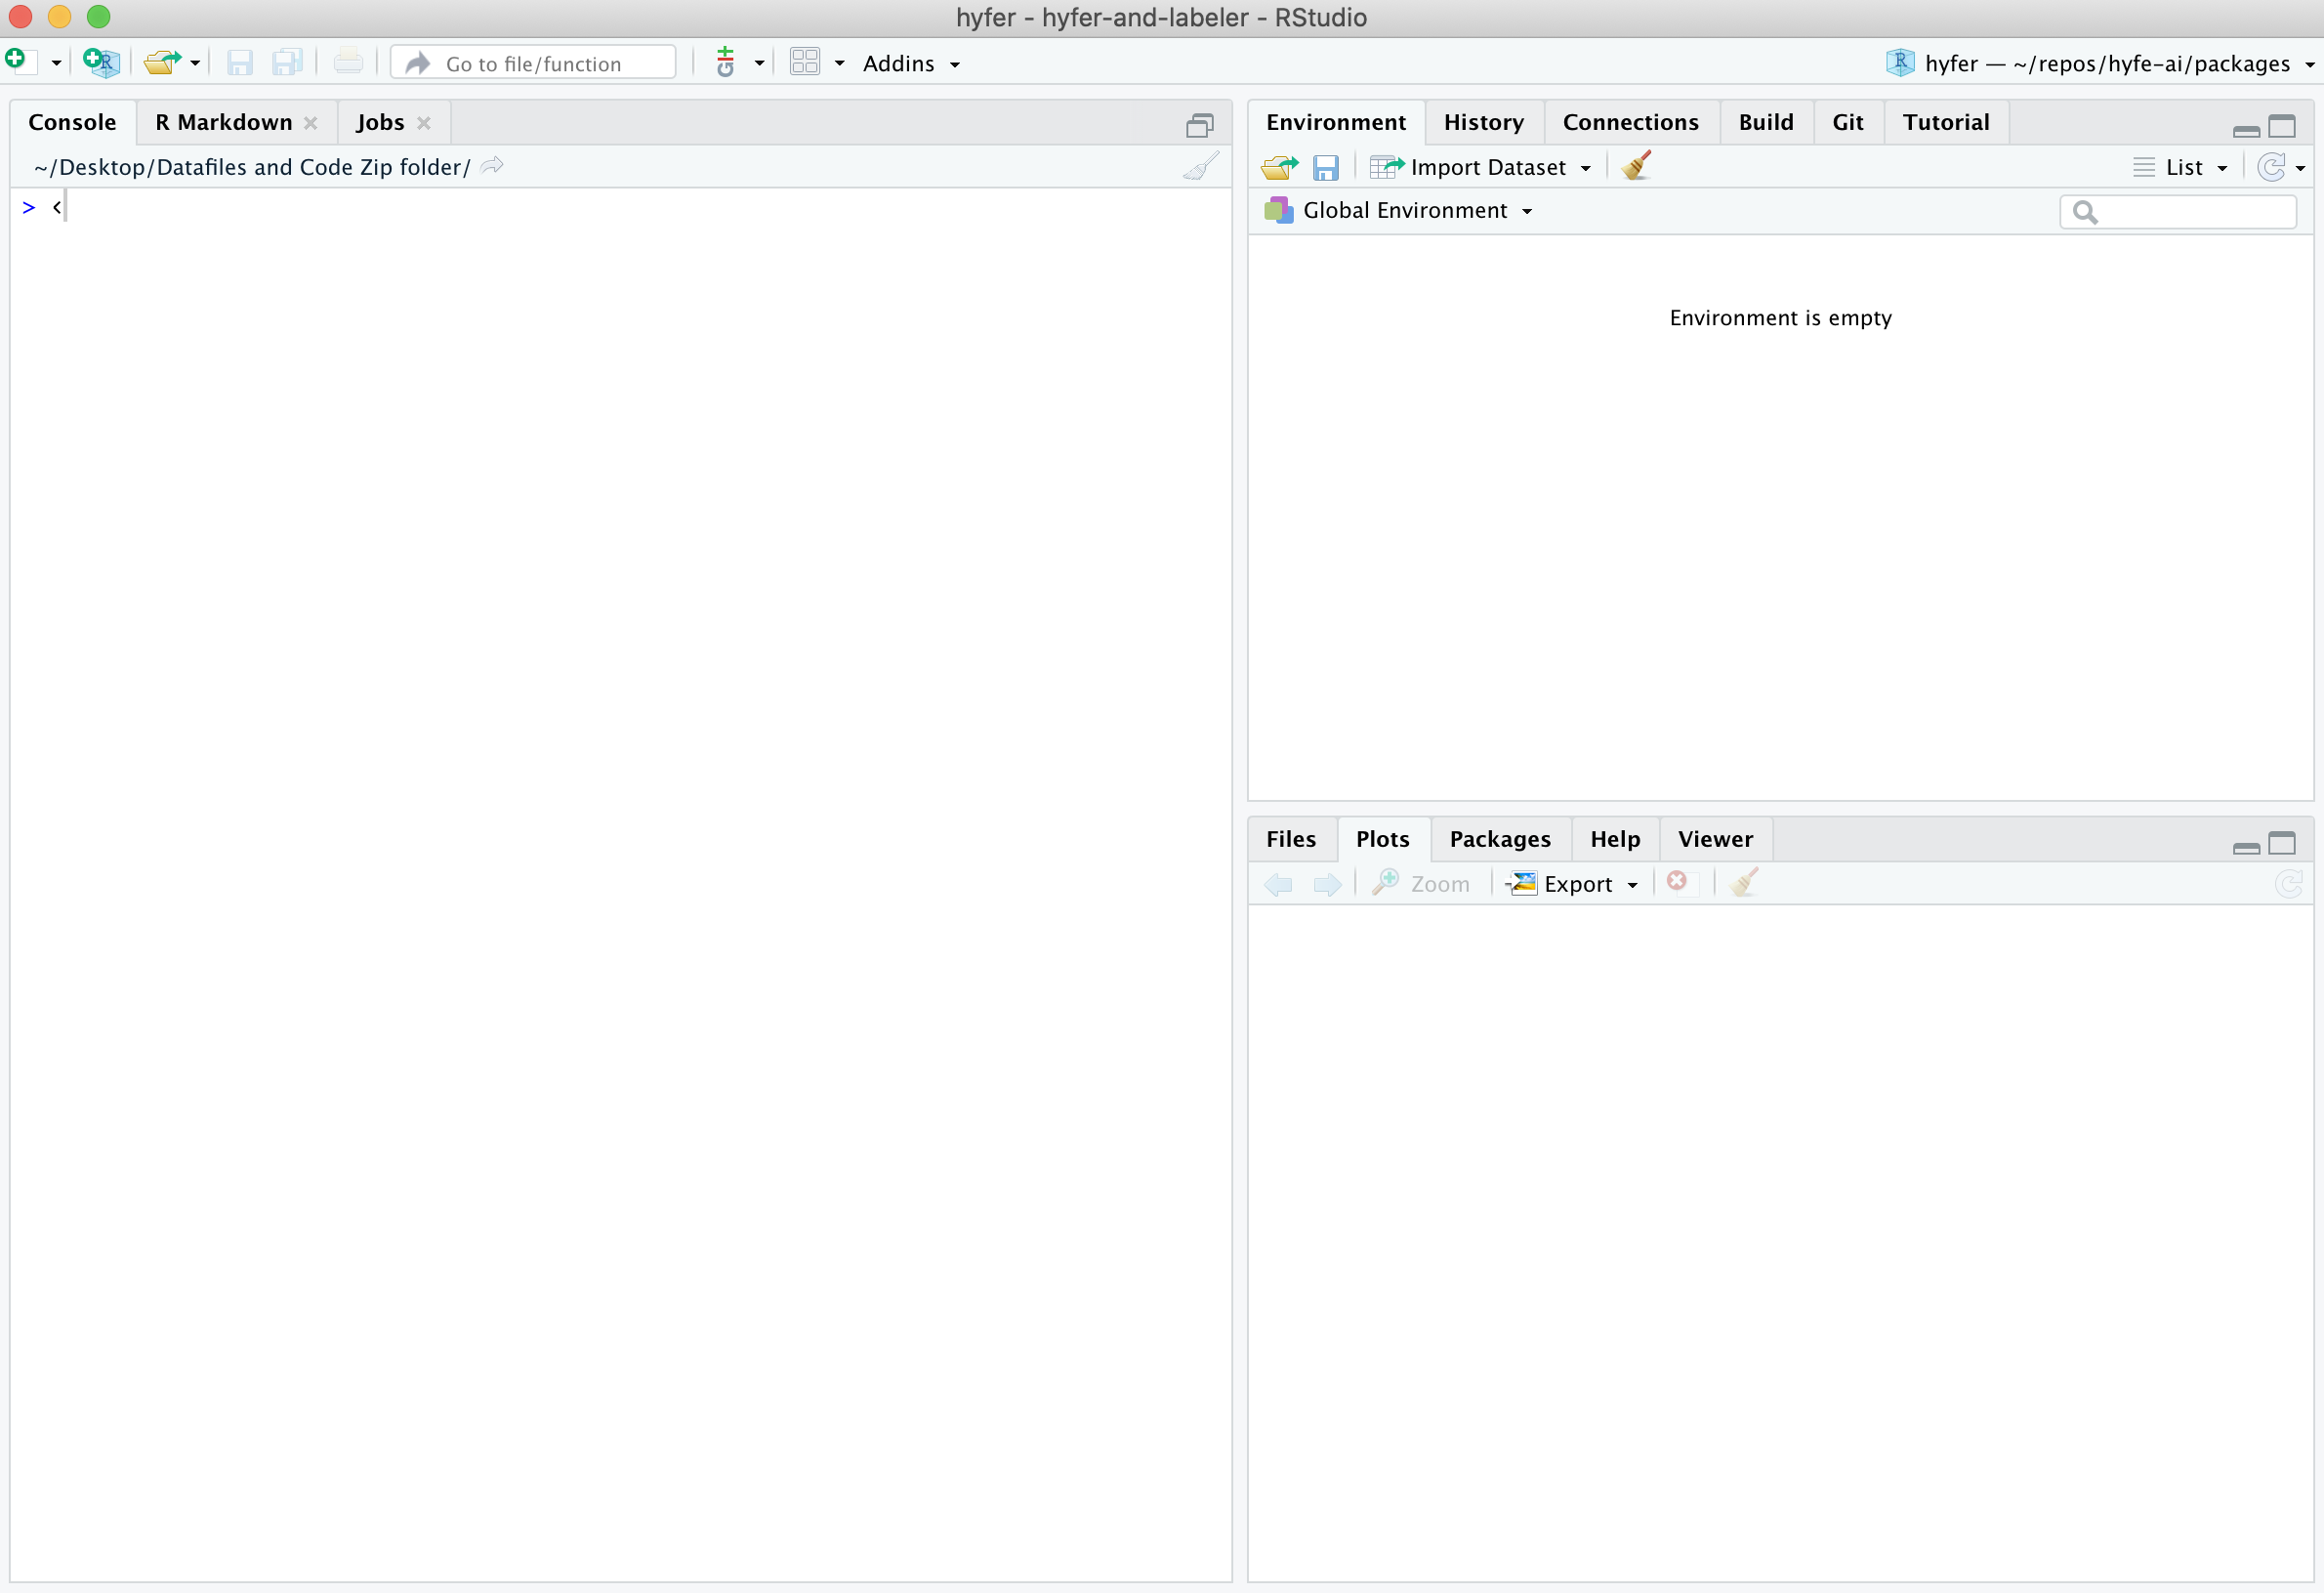
\includegraphics{img/rstudio_firstopen.png}

\textbf{Fourth, make sure \texttt{R} is running correctly in the background:}

In \texttt{RStudio}, in the pane on the left (the ``Console''), type 2+2 and hit Enter.\\
If \texttt{R} is working properly, the number ``4'' will be printed in the next line down.

\textbf{Finally, some minor adjustments to make \texttt{RStudio} run smoother (and look cooler):}

Go to \texttt{Tools\ \textgreater{}\ Global\ Options} and make sure your \texttt{General} settings match these exactly:

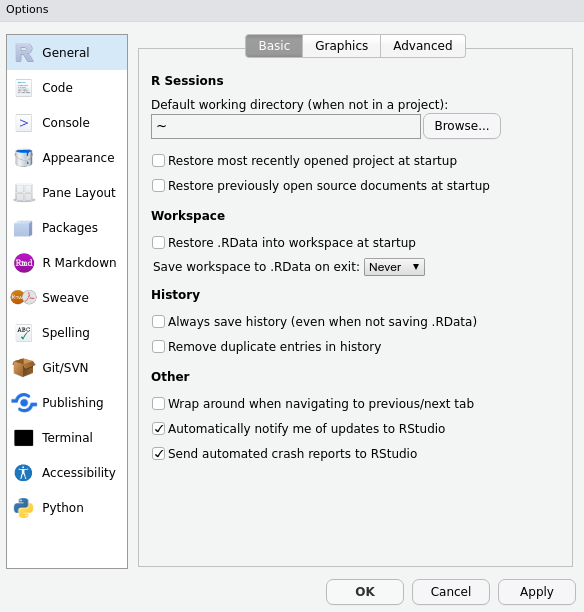
\includegraphics{img/rstudio_settings.png}

Specifically, \textbf{uncheck} the option under \emph{Workspace} to `Restore .RData into workspace at startup.'

Now go to the \texttt{Appearance} settings and choose a cool theme!

\includegraphics{img/rstudio_theme.png}

\textbf{Boom!}

\textbf{Appendix: Supplementary software}

In order to install certain packages, you might need to take some more steps.

\textbf{Install Git Bash on Windows}

\begin{itemize}
\tightlist
\item
  Visit \url{https://gitforwindows.org/} and follow the instructions for downloading and installation.
\end{itemize}

\textbf{Install developer tools}

\begin{itemize}
\tightlist
\item
  On Windows, download \url{http://cran.r-project.org/bin/windows/Rtools/} and run the installer.
\item
  On Mac, you need Xcode Command Line Tools. You might already have this. Check by running \texttt{devtools::has\_devel()}. If you don't have it, open shell/terminal and run
\end{itemize}

\begin{verbatim}
xcode-select --install
\end{verbatim}

\begin{itemize}
\tightlist
\item
  Alternatively, on Mac, you can download Xcode from the Mac App Store directly: \url{https://apps.apple.com/ca/app/xcode/id497799835?mt=12}
\end{itemize}

\hypertarget{running-r-code}{%
\chapter{Running R code}\label{running-r-code}}

\hypertarget{learning-goals}{%
\subsubsection*{Learning goals}\label{learning-goals}}
\addcontentsline{toc}{subsubsection}{Learning goals}

\begin{itemize}
\tightlist
\item
  Learn how to run code in R
\item
  Learn how to use R as a calculator
\item
  Learn how to use mathematical and logical operators in R
\end{itemize}

~

When you open \texttt{RStudio}, you see several different panes within the program's window. You will get a tour of \texttt{RStudio} in the next module. For now, look at the left half of the screen. You should see a large pane entitled the \emph{Console}.

\includegraphics{img/rstudio_firstopen.png}

\texttt{RStudio}'s \emph{Console} is your window into \texttt{R}, the engine under the hood. The \emph{Console} is where you type commands for \texttt{R} to run, and where \texttt{R} prints back the results of what you have told it to do. Think of the \emph{Console} as a chatroom, where you and \texttt{R} talk back and forth.

\hypertarget{running-code-in-the-console}{%
\section*{\texorpdfstring{Running code in the \emph{Console}}{Running code in the Console}}\label{running-code-in-the-console}}
\addcontentsline{toc}{section}{Running code in the \emph{Console}}

Type \texttt{1\ +\ 1} into the \emph{Console}, then press \texttt{Enter} --- you should get the following:

\begin{Shaded}
\begin{Highlighting}[]
\DecValTok{1} \SpecialCharTok{+} \DecValTok{1}
\CommentTok{\#\textgreater{} [1] 2}
\end{Highlighting}
\end{Shaded}

When you press \texttt{Enter}, you send your line of code to \texttt{R}; you post it for \texttt{R} to see. Then \texttt{R} takes it, does some processing, and posts a result (\texttt{2}) just below your command.

Note that spaces don't matter --- both of the following two commands are legible to \texttt{R} and return the same thing:

\begin{Shaded}
\begin{Highlighting}[]
\DecValTok{4}\SpecialCharTok{+}\DecValTok{4}
\CommentTok{\#\textgreater{} [1] 8}
\end{Highlighting}
\end{Shaded}

\begin{Shaded}
\begin{Highlighting}[]
\DecValTok{4}        \SpecialCharTok{+}        \DecValTok{4}
\CommentTok{\#\textgreater{} [1] 8}
\end{Highlighting}
\end{Shaded}

However, it is better to make your code as easy to read as possible, which usually means using a single space between numbers:

\begin{Shaded}
\begin{Highlighting}[]
\DecValTok{4} \SpecialCharTok{+} \DecValTok{4}
\CommentTok{\#\textgreater{} [1] 8}
\end{Highlighting}
\end{Shaded}

\hypertarget{use-r-like-a-calculator}{%
\section*{Use R like a calculator}\label{use-r-like-a-calculator}}
\addcontentsline{toc}{section}{Use R like a calculator}

At heart, \texttt{R} is really just a (very) fancy calculator. Some calculations are straightforward, like addition and subtraction:

\begin{Shaded}
\begin{Highlighting}[]
\DecValTok{490} \SpecialCharTok{+} \DecValTok{1000}
\CommentTok{\#\textgreater{} [1] 1490}
\end{Highlighting}
\end{Shaded}

\begin{Shaded}
\begin{Highlighting}[]
\DecValTok{490} \SpecialCharTok{{-}} \DecValTok{1000}
\CommentTok{\#\textgreater{} [1] {-}510}
\end{Highlighting}
\end{Shaded}

Division is pretty straightfoward too:

\begin{Shaded}
\begin{Highlighting}[]
\DecValTok{24} \SpecialCharTok{/} \DecValTok{2}
\CommentTok{\#\textgreater{} [1] 12}
\end{Highlighting}
\end{Shaded}

For multiplication, use an asterisk (\texttt{*}):

\begin{Shaded}
\begin{Highlighting}[]
\DecValTok{24} \SpecialCharTok{*} \DecValTok{2}
\CommentTok{\#\textgreater{} [1] 48}
\end{Highlighting}
\end{Shaded}

You denote exponents like this:

\begin{Shaded}
\begin{Highlighting}[]
\DecValTok{2}\SpecialCharTok{\^{}}\DecValTok{2}
\CommentTok{\#\textgreater{} [1] 4}
\end{Highlighting}
\end{Shaded}

\begin{Shaded}
\begin{Highlighting}[]
\DecValTok{2}\SpecialCharTok{\^{}}\DecValTok{3}
\CommentTok{\#\textgreater{} [1] 8}
\end{Highlighting}
\end{Shaded}

\begin{Shaded}
\begin{Highlighting}[]
\DecValTok{2}\SpecialCharTok{\^{}}\DecValTok{4}
\CommentTok{\#\textgreater{} [1] 16}
\end{Highlighting}
\end{Shaded}

Finally, note that \texttt{R} is fine with negative numbers:

\begin{Shaded}
\begin{Highlighting}[]
\DecValTok{9} \SpecialCharTok{+} \SpecialCharTok{{-}}\DecValTok{100}
\CommentTok{\#\textgreater{} [1] {-}91}
\end{Highlighting}
\end{Shaded}

\hypertarget{getting-along-with-r}{%
\section*{\texorpdfstring{Getting along with \texttt{R}}{Getting along with R}}\label{getting-along-with-r}}
\addcontentsline{toc}{section}{Getting along with \texttt{R}}

\hypertarget{re-running-code-in-the-console}{%
\subsection*{\texorpdfstring{Re-running code in the \emph{Console}}{Re-running code in the Console}}\label{re-running-code-in-the-console}}
\addcontentsline{toc}{subsection}{Re-running code in the \emph{Console}}

If you want to re-run the code you just ran, or if you want to recall the code so that you can adjust it slightly, click anywhere in the \emph{Console} then press your keyboard's \texttt{Up} arrow.

If you keep pressing your \texttt{Up} arrow, \texttt{R} will present you with sequentially older commands. \texttt{R} keeps a history of everything you have said to it since you opened this window.

If you accidentally recalled an old command without meaning to, you can reset the \emph{Console}'s command line by pressing \texttt{Escape}.

\hypertarget{incomplete-commands}{%
\subsection*{Incomplete commands}\label{incomplete-commands}}
\addcontentsline{toc}{subsection}{Incomplete commands}

\texttt{R} gets confused when you enter an incomplete command, and will wait for you to write the remainder of your command on the next line in the \emph{Console} before doing anything.

For example, try running this code in your \emph{Console}:

\begin{Shaded}
\begin{Highlighting}[]
\DecValTok{45} \SpecialCharTok{+}
\end{Highlighting}
\end{Shaded}

You will find that \texttt{R} gives you a little \texttt{+} sign on the line under your command, which means it is waiting for you to complete your command.

If you want to complete your command, add a number (e.g., \texttt{3)} and hit \texttt{Enter}. You should now be given an answer (e.g., \texttt{48}).

Or, if instead you want \texttt{R} to stop waiting and stop running, just press the \texttt{Escape} key.

\hypertarget{semicolons}{%
\subsection*{Semicolons}\label{semicolons}}
\addcontentsline{toc}{subsection}{Semicolons}

Semicolons can be used to put two separate commands on the same line of code. For example, these two lines of commands \ldots{}

\begin{Shaded}
\begin{Highlighting}[]
\DecValTok{4} \SpecialCharTok{+} \DecValTok{5}
\CommentTok{\#\textgreater{} [1] 9}
\DecValTok{6} \SpecialCharTok{+} \DecValTok{10}
\CommentTok{\#\textgreater{} [1] 16}
\end{Highlighting}
\end{Shaded}

.. will return the same results as this single line of commands:

\begin{Shaded}
\begin{Highlighting}[]
\DecValTok{4} \SpecialCharTok{+} \DecValTok{5}\NormalTok{ ; }\DecValTok{6} \SpecialCharTok{+} \DecValTok{10}
\CommentTok{\#\textgreater{} [1] 9}
\CommentTok{\#\textgreater{} [1] 16}
\end{Highlighting}
\end{Shaded}

This will become a useful trick in a few modules downstream.

\hypertarget{getting-errors}{%
\subsection*{Getting errors}\label{getting-errors}}
\addcontentsline{toc}{subsection}{Getting errors}

\texttt{R} only understands your commands if they follow the rules of the \texttt{R} language (often referred to as its \emph{syntax}). If \texttt{R} does not understand your code, it will throw an error and give up on trying to execute that line of code.

For example, try running this code in your \emph{Console}:

\begin{Shaded}
\begin{Highlighting}[]
\DecValTok{4} \SpecialCharTok{+}\NormalTok{ y}
\end{Highlighting}
\end{Shaded}

You probably received a message in red font stating: \texttt{Error:\ object\ \textquotesingle{}y\textquotesingle{}\ not\ found}. That is because \texttt{R} did know how to interpret the symbol \texttt{y} in this case, so it just gave up.

\textbf{Get used to errors!} They happen all the time, even (especially?) to professionals, and it is essential that you get used to reading your own code to find and fix its errors.

Here's another piece of code that will produce an error:

\begin{Shaded}
\begin{Highlighting}[]
\NormalTok{dfjkltr9fitwt985ut9e3}
\end{Highlighting}
\end{Shaded}

\hypertarget{using-parentheses}{%
\subsection*{Using parentheses}\label{using-parentheses}}
\addcontentsline{toc}{subsection}{Using parentheses}

\texttt{R} is usually great about following classic rules for Order of Operations, and you can use parentheses to exert control over that order. For example, these two commands produce different results:

\begin{Shaded}
\begin{Highlighting}[]
\DecValTok{2}\SpecialCharTok{*}\DecValTok{7} \SpecialCharTok{{-}} \DecValTok{2}\SpecialCharTok{*}\DecValTok{5} \SpecialCharTok{/} \DecValTok{2}
\CommentTok{\#\textgreater{} [1] 9}
\end{Highlighting}
\end{Shaded}

\begin{Shaded}
\begin{Highlighting}[]
\NormalTok{(}\DecValTok{2}\SpecialCharTok{*}\DecValTok{7} \SpecialCharTok{{-}} \DecValTok{2}\SpecialCharTok{*}\DecValTok{5}\NormalTok{) }\SpecialCharTok{/} \DecValTok{2}
\CommentTok{\#\textgreater{} [1] 2}
\end{Highlighting}
\end{Shaded}

Note that parentheses need to come in pairs: whenever you type an open parenthesis, \texttt{(}, eventually you need to provide a corresponding closed parenthesis, \texttt{)}.

The following line of code will return a plus sign, \texttt{+}, since \texttt{R} is waiting for you to close the parenthetical before it processes your command:

\begin{Shaded}
\begin{Highlighting}[]
\DecValTok{4} \SpecialCharTok{+}\NormalTok{ (}\DecValTok{5}
\end{Highlighting}
\end{Shaded}

Remember: \textbf{parentheses come in pairs!} The same goes for other types of brackets: \texttt{\{...\}} and \texttt{{[}...{]}}.

\hypertarget{using-operators-in-r}{%
\subsection*{Using operators in R}\label{using-operators-in-r}}
\addcontentsline{toc}{subsection}{Using operators in R}

You can ask \texttt{R} basic questions using \emph{operators}.

For example, you can ask whether two values are equal to each other.

\begin{Shaded}
\begin{Highlighting}[]
\DecValTok{96} \SpecialCharTok{==} \DecValTok{95}
\CommentTok{\#\textgreater{} [1] FALSE}
\end{Highlighting}
\end{Shaded}

\begin{Shaded}
\begin{Highlighting}[]
\DecValTok{95} \SpecialCharTok{+} \DecValTok{2} \SpecialCharTok{==} \DecValTok{95} \SpecialCharTok{+} \DecValTok{2}
\CommentTok{\#\textgreater{} [1] TRUE}
\end{Highlighting}
\end{Shaded}

\texttt{R} is telling you that the first statement is \texttt{FALSE} (\texttt{96} is not, in fact, equal to \texttt{95}) and that the second statement is \texttt{TRUE} (\texttt{95\ +\ 2} is, in fact, equal to itself).

\textbf{Note the use of \emph{double} equal signs here.} You must use two of them in order for \texttt{R} to understand that you are asking for this logical test.

You can also ask if two values are \emph{NOT} equal to each other:

\begin{Shaded}
\begin{Highlighting}[]
\DecValTok{96} \SpecialCharTok{!=} \DecValTok{95}
\CommentTok{\#\textgreater{} [1] TRUE}
\end{Highlighting}
\end{Shaded}

\begin{Shaded}
\begin{Highlighting}[]
\DecValTok{95} \SpecialCharTok{+} \DecValTok{2} \SpecialCharTok{!=} \DecValTok{95} \SpecialCharTok{+} \DecValTok{2}
\CommentTok{\#\textgreater{} [1] FALSE}
\end{Highlighting}
\end{Shaded}

This test is a bit more difficult to understand: In the first statement, \texttt{R} is telling you that it is \texttt{TRUE} that \texttt{96} is different from \texttt{95}. In the second statement, \texttt{R} is saying that it is \texttt{FALSE} that \texttt{95\ +\ 2} is not the same as itself.

Note that \texttt{R} lets you write these tests another, even more confusing way:

\begin{Shaded}
\begin{Highlighting}[]
\SpecialCharTok{!} \DecValTok{96} \SpecialCharTok{==} \DecValTok{95}
\CommentTok{\#\textgreater{} [1] TRUE}
\end{Highlighting}
\end{Shaded}

\begin{Shaded}
\begin{Highlighting}[]
\SpecialCharTok{!} \DecValTok{95} \SpecialCharTok{+} \DecValTok{2} \SpecialCharTok{==} \DecValTok{95} \SpecialCharTok{+} \DecValTok{2}
\CommentTok{\#\textgreater{} [1] FALSE}
\end{Highlighting}
\end{Shaded}

The first line of code is asking \texttt{R} whether it is not true that \texttt{96} and \texttt{95} are equal to each other, which is \texttt{TRUE}. The second line of code is asking \texttt{R} whether it is not true that \texttt{95\ +\ 2} is the same as itself, which is of course \texttt{FALSE}.

Other commonly used operators in \texttt{R} include greater than / less than symbols (\texttt{\textgreater{}} and \texttt{\textless{}}, also known as the \emph{left-facing alligator} and \emph{right-facing alligator}), and greater/less than or equal to (\texttt{\textgreater{}=} and \texttt{\textless{}=}).

\begin{Shaded}
\begin{Highlighting}[]
\DecValTok{100} \SpecialCharTok{\textgreater{}} \DecValTok{100}
\CommentTok{\#\textgreater{} [1] FALSE}
\end{Highlighting}
\end{Shaded}

\begin{Shaded}
\begin{Highlighting}[]
\DecValTok{100} \SpecialCharTok{\textgreater{}=} \DecValTok{100}
\CommentTok{\#\textgreater{} [1] TRUE}
\end{Highlighting}
\end{Shaded}

\begin{Shaded}
\begin{Highlighting}[]
\NormalTok{(}\DecValTok{100} \SpecialCharTok{!=} \DecValTok{100}\NormalTok{) }\SpecialCharTok{==} \ConstantTok{FALSE}
\CommentTok{\#\textgreater{} [1] TRUE}
\end{Highlighting}
\end{Shaded}

\hypertarget{use-built-in-r-functions}{%
\subsection*{\texorpdfstring{Use built-in \texttt{R} functions}{Use built-in R functions}}\label{use-built-in-r-functions}}
\addcontentsline{toc}{subsection}{Use built-in \texttt{R} functions}

\texttt{R} has some built-in ``functions'' for common calculations, such as finding square roots and logarithms. Functions are packages of code that take a given value, transform it according to some internal code instructions, and provide an output. As you learn more about \texttt{R}, you will learn to write your very own functions; for starters, though, let's just learn to use some functions that \texttt{R} provides. To find the square-root of a number, for example, use the function \texttt{sqrt()}:

\begin{Shaded}
\begin{Highlighting}[]
\FunctionTok{sqrt}\NormalTok{(}\DecValTok{16}\NormalTok{)}
\CommentTok{\#\textgreater{} [1] 4}
\end{Highlighting}
\end{Shaded}

Note the use of parentheses here. When you are calling a function, when you see parentheses, think of the word `of' --- you are taking the \texttt{sqrt} \textbf{of} the number inside the parentheses.

To get the natural (base \(e\)) logarithm of a number, use \texttt{log()}:

\begin{Shaded}
\begin{Highlighting}[]
\FunctionTok{log}\NormalTok{(}\DecValTok{4}\NormalTok{)}
\CommentTok{\#\textgreater{} [1] 1.386294}
\end{Highlighting}
\end{Shaded}

This is the value that \(e\) must be raised to to equal 4; we'll see the value of \(e\) and check \(e^{\log{4}}\) below. To calculate a common (base 10) logarithm instead, use \texttt{log10(\ )}:

\begin{Shaded}
\begin{Highlighting}[]
\FunctionTok{log10}\NormalTok{(}\DecValTok{10}\NormalTok{)}
\CommentTok{\#\textgreater{} [1] 1}
\end{Highlighting}
\end{Shaded}

Another handy function is \texttt{round()}, for rounding numbers to a specific number of decimal places.

\begin{Shaded}
\begin{Highlighting}[]
\DecValTok{100}\SpecialCharTok{/}\DecValTok{3}
\CommentTok{\#\textgreater{} [1] 33.33333}
\end{Highlighting}
\end{Shaded}

\begin{Shaded}
\begin{Highlighting}[]
\FunctionTok{round}\NormalTok{(}\DecValTok{100}\SpecialCharTok{/}\DecValTok{3}\NormalTok{)}
\CommentTok{\#\textgreater{} [1] 33}
\end{Highlighting}
\end{Shaded}

\begin{Shaded}
\begin{Highlighting}[]
\FunctionTok{round}\NormalTok{(}\DecValTok{100}\SpecialCharTok{/}\DecValTok{3}\NormalTok{,}\AttributeTok{digits=}\DecValTok{1}\NormalTok{)}
\CommentTok{\#\textgreater{} [1] 33.3}
\end{Highlighting}
\end{Shaded}

\begin{Shaded}
\begin{Highlighting}[]
\FunctionTok{round}\NormalTok{(}\DecValTok{100}\SpecialCharTok{/}\DecValTok{3}\NormalTok{,}\AttributeTok{digits=}\DecValTok{2}\NormalTok{)}
\CommentTok{\#\textgreater{} [1] 33.33}
\end{Highlighting}
\end{Shaded}

\begin{Shaded}
\begin{Highlighting}[]
\FunctionTok{round}\NormalTok{(}\DecValTok{100}\SpecialCharTok{/}\DecValTok{3}\NormalTok{,}\AttributeTok{digits=}\DecValTok{3}\NormalTok{)}
\CommentTok{\#\textgreater{} [1] 33.333}
\end{Highlighting}
\end{Shaded}

Finally, \texttt{R} also comes with some built-in \emph{values}, such as \(\pi\) :

\begin{Shaded}
\begin{Highlighting}[]
\NormalTok{pi}
\CommentTok{\#\textgreater{} [1] 3.141593}
\end{Highlighting}
\end{Shaded}

Some values you might want to use are not built in, but are easy to get with a built-in function. For example,
use \texttt{exp()} to get powers of \(e\) (the base of the natural logarithm) :

\begin{Shaded}
\begin{Highlighting}[]
\FunctionTok{exp}\NormalTok{(}\DecValTok{1}\NormalTok{)}
\CommentTok{\#\textgreater{} [1] 2.718282}
\end{Highlighting}
\end{Shaded}

\begin{Shaded}
\begin{Highlighting}[]
\FunctionTok{exp}\NormalTok{(}\FunctionTok{log}\NormalTok{(}\DecValTok{4}\NormalTok{))}
\CommentTok{\#\textgreater{} [1] 4}
\end{Highlighting}
\end{Shaded}

\hypertarget{exercises}{%
\subsubsection*{Exercises}\label{exercises}}
\addcontentsline{toc}{subsubsection}{Exercises}

\textbf{Use \texttt{R} like a calculator}

\textbf{1.} Type a command in the \emph{Console} to determine the sum of 596 and 198.

\textbf{2.} Re-run the sum of 596 and 198 without re-typing it.

\textbf{3.} Recall the command again, but this time adjust the code to find the sum of 596 and 298.

\textbf{4.} Practice escaping an accidentally called command: recall your most recent command, then press the right key to clear the \emph{Console}'s command line.

~\\
\textbf{Recalling commands}

\textbf{5.} Find the sum of the ages of everyone in your immediate family.

\textbf{6.} Now recall that command and adjust it to determine the \emph{average} age of the members of your family.

\textbf{7.} Find the square root of \(\pi\) and round the answer to the 2 decimal places.

~

\textbf{Finding errors}

\textbf{8.} This line of code won't run; instead, \texttt{R} will wait for more with a \texttt{+} symbol. Find the problem and re-write the code so that it works.

\begin{Shaded}
\begin{Highlighting}[]
\DecValTok{5} \SpecialCharTok{*} \DecValTok{6} \SpecialCharTok{+}
\end{Highlighting}
\end{Shaded}

\textbf{9.} The same goes for this line of code. Fix it, too.

\begin{Shaded}
\begin{Highlighting}[]
\FunctionTok{sqrt}\NormalTok{(}\DecValTok{16}
\end{Highlighting}
\end{Shaded}

\textbf{10.} This line of code will trigger an error. Find the problem and re-write the code so that it works.

\begin{Shaded}
\begin{Highlighting}[]
\FunctionTok{round}\NormalTok{(}\DecValTok{100}\SpecialCharTok{/}\DecValTok{3}\NormalTok{,digits}\SpecialCharTok{+}\DecValTok{3}\NormalTok{)}
\end{Highlighting}
\end{Shaded}

\textbf{11.} Type a command of your own into R that throws an error, then recall the command and revise so that \texttt{R} can understand it.

~

\textbf{Show that the following statements are TRUE:}

\textbf{12.} \(\pi\) is greater than the square root of 9

\textbf{13.} It is FALSE that the square root of 9 is greater than \(\pi\)

\textbf{14.} \(\pi\) rounded to the nearest whole number equals the square root of 9

~

\textbf{Asking \texttt{TRUE} / \texttt{FALSE} questions}

\textbf{15.} Write and run a line of code that asks whether these two calculations return the same result:

\begin{Shaded}
\begin{Highlighting}[]
\DecValTok{2}\SpecialCharTok{*}\DecValTok{7} \SpecialCharTok{{-}} \DecValTok{2}\SpecialCharTok{*}\DecValTok{5} \SpecialCharTok{/} \DecValTok{2}
\end{Highlighting}
\end{Shaded}

\begin{Shaded}
\begin{Highlighting}[]
\NormalTok{(}\DecValTok{2}\SpecialCharTok{*}\DecValTok{7} \SpecialCharTok{{-}} \DecValTok{2}\SpecialCharTok{*}\DecValTok{5}\NormalTok{) }\SpecialCharTok{/} \DecValTok{2}
\CommentTok{\#\textgreater{} [1] 2}
\end{Highlighting}
\end{Shaded}

\textbf{16.} Now write and run a line of code that asks whether the first calculation is larger than the second:

~

\hypertarget{other-resources}{%
\subsubsection*{Other Resources}\label{other-resources}}
\addcontentsline{toc}{subsubsection}{Other Resources}

Hobbes Primer, Table 1 (Math Operators, pg. 18) and Table 2 (Logical operators, pg. 22)

\hypertarget{using-rstudio-r-scripts}{%
\chapter{\texorpdfstring{Using \texttt{RStudio} \& \texttt{R} scripts}{Using RStudio \& R scripts}}\label{using-rstudio-r-scripts}}

\hypertarget{learning-goals-1}{%
\subsubsection*{Learning goals}\label{learning-goals-1}}
\addcontentsline{toc}{subsubsection}{Learning goals}

\begin{itemize}
\tightlist
\item
  Understand the difference between \texttt{R} and \texttt{RStudio}
\item
  Understand the \texttt{RStudio} working environment and window panes\\
\item
  Understand what \texttt{R} scripts are, and how to create and save them
\item
  Understand how to add comments to your code, and why doing so is important
\item
  Understand what a \emph{working directory} is, and how to use it
\item
  Learn basic project work flow
\end{itemize}

\hypertarget{r-and-rstudio-whats-the-difference}{%
\section*{\texorpdfstring{\texttt{R} and \texttt{RStudio}: what's the difference?}{R and RStudio: what's the difference?}}\label{r-and-rstudio-whats-the-difference}}
\addcontentsline{toc}{section}{\texttt{R} and \texttt{RStudio}: what's the difference?}

These two entities are similar, but it is important to understand how they are different.

In short, \texttt{R} is an open-source (i.e., free) coding language: a powerful programming engine that can be used to do really cool things with data.

\texttt{R\ Studio}, in contrast, is a free \emph{user interface} that helps you interact with \texttt{R}. If you think of \texttt{R} as an engine, then it helps to think of \texttt{RStudio} as the car that contains it. Like a car,\texttt{RStudio} makes it easier and more comfortable to use the engine to get where you want to go.

\texttt{R\ Studio} needs \texttt{R} in order to function, but \texttt{R} can technically be used on its own outside of \texttt{RStudio} if you want. However, just as a good car mechanic can get an engine to run without being installed within a car, using \texttt{R} on its own is a bit clunky and requires some expertise. For beginners (and everyone else, really), \texttt{R} is just so much more pleasant to use when you are operating it from within \texttt{RStudio}.

\texttt{RStudio} also has increasingly powerful \emph{extensions} that make \texttt{R} even more useful and versatile in data science. These extensions allow you to use \texttt{R} to make interactive data dashboards, beautiful and reproducible data reports, presentations, websites, and even books. And new features like these are regularly being added to \texttt{RStudio} by its all-star team of data scientists.

That is why this book \emph{always} uses \texttt{RStudio} when working with \texttt{R}.

\hypertarget{two-minute-tour-of-rstudio}{%
\section*{\texorpdfstring{Two-minute tour of \texttt{RStudio}}{Two-minute tour of RStudio}}\label{two-minute-tour-of-rstudio}}
\addcontentsline{toc}{section}{Two-minute tour of \texttt{RStudio}}

When you open \texttt{RStudio} for the first time, you will see a window that looks like the screenshot below.

\includegraphics{img/rstudio_windows.png}

\hypertarget{console}{%
\subsection*{Console}\label{console}}
\addcontentsline{toc}{subsection}{Console}

You are already acquainted with \texttt{RStudio}'s \emph{Console}, the window pane on the left that you use to ``talk'' to \texttt{R}. (See the previous module.)

\hypertarget{environment}{%
\subsection*{Environment}\label{environment}}
\addcontentsline{toc}{subsection}{Environment}

In the top right pane, the \emph{Environment}, \texttt{RStudio} will maintain a list of all the datasets, variables, and functions that you are using as you work. The next modules will explain what variables and functions are.

\hypertarget{files-plots-packages-help}{%
\subsection*{Files, Plots, Packages, \& Help}\label{files-plots-packages-help}}
\addcontentsline{toc}{subsection}{Files, Plots, Packages, \& Help}

You will use the bottom right pane very often.

\begin{itemize}
\tightlist
\item
  The \textbf{Files} tab lets you see all the files within your \textbf{working directory}, which will be explained in the section below.\\
\item
  The \textbf{Plots} tab lets you see the plots you are producing with your code.\\
\item
  The \textbf{Packages} tab lets you see the \emph{packages} you currently have installed on your computer. Packages are bundles of \texttt{R} functions downloaded from the internet; they will be explained in detail a few modules down the road.\\
\item
  The \textbf{Help} tab is very important! It lets you see \emph{documentation} (i.e., user's guides) for the functions you use in your code. Functions will also be explained in detail a few modules down the road.
\end{itemize}

These three panes are useful, but the most useful window pane of all is actually \emph{missing} when you first open \texttt{RStudio}. This important pane is where you work with \textbf{scripts}.

\hypertarget{scripts}{%
\section*{Scripts}\label{scripts}}
\addcontentsline{toc}{section}{Scripts}

Before explaining what scripts are and why they are awesome, let's start a new script.

\textbf{To start a new script,} go to the top left icon in the \texttt{RStudio} window, and click on the green plus sign with a blank page behind it:

\includegraphics{img/rstudio_newscript.png}

A dropdown window will appear. Select ``R Script''.

A new window pane will then appear in the top left quadrant of your \texttt{RStudio} window:

\includegraphics{img/rstudio_scripts.png}
You now have a blank script to work in!

Now type some simple commands into your script:

\begin{Shaded}
\begin{Highlighting}[]
\DecValTok{2}  \SpecialCharTok{+} \DecValTok{10}
\DecValTok{16} \SpecialCharTok{*} \DecValTok{32}
\end{Highlighting}
\end{Shaded}

Notice that when you press \texttt{Enter} after each line of code, nothing happens in the \emph{Console}. In order to send this code to the Console, press \texttt{Enter\ +\ Command} at the same time (or \texttt{Enter\ +\ Control}, if you are on Windows) for each line of code.

To send both lines of code to the \emph{Console} at once, select both lines of code and hit \texttt{Enter\ +\ Command}.

(To select multiple lines of code, you can (1) click and drag with your mouse or (2) hold down your \texttt{Shift} key while clicking your down arrow key. To select \emph{all} lines of code, press \texttt{Command\ +\ A}.)

So let's build up this script. Add a few more lines to your script, such that your script now looks like this.

\begin{Shaded}
\begin{Highlighting}[]
\DecValTok{2}  \SpecialCharTok{+} \DecValTok{10}
\DecValTok{16} \SpecialCharTok{*} \DecValTok{32}
\DecValTok{1080} \SpecialCharTok{/} \DecValTok{360}
\DecValTok{500} \SpecialCharTok{{-}} \DecValTok{600}
\end{Highlighting}
\end{Shaded}

Run all of these lines of code at once.

Now add \texttt{10} to the first number in each row, and re-run all of the code.

Think about how much more efficient part (B) was thanks to your script! If you had typed all of that directly into your \emph{Console}, you would have to recall or retype each line individually. That difference builds up when your number of commands grows into the hundreds.

\hypertarget{what-is-an-r-script-and-why-are-scripts-so-awesome}{%
\subsection*{\texorpdfstring{What is an \texttt{R} script, and why are scripts so awesome?}{What is an R script, and why are scripts so awesome?}}\label{what-is-an-r-script-and-why-are-scripts-so-awesome}}
\addcontentsline{toc}{subsection}{What is an \texttt{R} script, and why are scripts so awesome?}

An \texttt{R} script is a file where you can keep a record of your code. Just as a script tells actors exactly what to say and when to say it, an \texttt{R} script tells \texttt{R} exactly what code to run, and in what order to run it.

When working with R, you will almost always type your code into a script first, \emph{then} send it to the \emph{Console}. You can run your code immediately using \texttt{Enter\ +\ Command}, but you also have a script of what you have done so that you can run the exact same code at a later time

To understand why \texttt{R} scripts are so awesome, consider a typical workflow in \emph{Excel} or \emph{Google Sheets}. You open a big complicated spreadsheet, spend hours making changes, and save your changes frequently throughout your work session.

The main disadvantages of this workflow are :

\begin{enumerate}
\def\labelenumi{\arabic{enumi}.}
\item
  There is no detailed record of the changes you have made. You cannot prove that you have made changes correctly. You cannot pass the original dataset to someone else and ask them to revise it in the same way you have. (Nor would you want to, since making all those changes was so time-consuming!) Nor could you take a different dataset and guarantee that you are able to apply the exact same changes that you applied to the first. In other words, your work is not reproducible.
\item
  Making those changes is labor-intensive! Rather than spend time manually making changes to a single spreadsheet, it would be better to devote that energy to writing \texttt{R} code that makes those changes for you. That code could be run in this one case, but it could also be run at any later time, or easily modified to make similar changes to other spreadsheets.
\item
  Unless you are an advanced \emph{Excel} programmer, you are probably modifying your original dataset, which is always dangerous and a big No-No in data science. Each time you save your work in \emph{Excel} or \emph{Google Sheets} (which automatically saves each change you make), the original spreadsheet file gets replaced by the updated version. But if you brought your dataset into \texttt{R} instead, and modified it using an \texttt{R} script, then you leave the raw data alone and keep it safe. (Sure, you can always save different versions of your Excel file, but then you run the risk of mixing up versions and getting confused.)
\end{enumerate}

Working with \texttt{R} scripts allows you to avoid all of these pitfalls. When you write an \texttt{R} script, you are making your work \ldots.

\begin{itemize}
\item
  \textbf{Efficient.} Once you get comfortable writing \texttt{R} code, you will be able to write scripts in a few minutes. Those scripts can modify datasets within seconds (or less) in ways that would take hours (or years) to carry out manually in \emph{Excel} or \emph{Google Sheets}.
\item
  \textbf{Reproducible.} Once you have written an\texttt{R} script, you can reproduce your own work whenever you want to. You can send your script to a colleague so that they can reproduct your work as well. Reproducible work is defensible work.
\item
  \textbf{Low-risk.} Since your R script does not make any changes to the original data, you are keeping your data safe. It is \emph{essential} to preserve the sanctity of raw data!
\end{itemize}

Note that there is nothing fancy or special about an \texttt{R} script. An \texttt{R} script is a simple text file; that is, it only accepts basic text; you can't add images or change font style or font size in an \texttt{R} script; just letters, numbers, and your other keyboard keys. The file's extension, \texttt{.R} tells your computer to interpret that text as \texttt{R} code.

\hypertarget{commenting-your-code}{%
\subsection*{Commenting your code}\label{commenting-your-code}}
\addcontentsline{toc}{subsection}{Commenting your code}

Another advantage of scripts is that you can include \emph{comments} throughout your code to explain what you are doing and why. A \emph{comment} is just a part of your script that is useful to you but that is ignored by \texttt{R}.

To add comments to your code, use the hashtag symbol (\texttt{\#}). Any text following a \texttt{\#} will be ignored by \texttt{R}.

Here is the script above, now with comments added:

\begin{Shaded}
\begin{Highlighting}[]
\CommentTok{\# Define variable x}
\NormalTok{x }\OtherTok{\textless{}{-}} \DecValTok{2} 
\NormalTok{x}

\CommentTok{\# Make a new variable, y, based on x}
\NormalTok{y }\OtherTok{\textless{}{-}}\NormalTok{ x}\SpecialCharTok{*}\DecValTok{56}

\NormalTok{z }\OtherTok{\textless{}{-}}\NormalTok{ y }\SpecialCharTok{/} \DecValTok{23} \CommentTok{\# Make a third variable, z, based on y}
 
\NormalTok{x }\SpecialCharTok{+}\NormalTok{ y }\SpecialCharTok{+}\NormalTok{ z }\CommentTok{\# Now get the sum of all three variables}
\end{Highlighting}
\end{Shaded}

Adding comments can be more work, but in the end it saves you time and makes your code more effective. Comments might not seem necessary in the moment, but it is amazing how helpful they are when you come back to your code the next day. Frequent and helpful comments make the difference between good and great code. Comment early, comment often!

You can also use lines of hashtags to visually organize your code. For example:

\begin{Shaded}
\begin{Highlighting}[]
\DocumentationTok{\#\#\#\#\#\#\#\#\#\#\#\#\#\#\#\#\#\#\#\#\#\#\#\#\#\#\#\#\#\#\#\#\#\#\#\#\#\#\#\#\#\#\#\#\#\#}
\CommentTok{\# Setup}
\DocumentationTok{\#\#\#\#\#\#\#\#\#\#\#\#\#\#\#\#\#\#\#\#\#\#\#\#\#\#\#\#\#\#\#\#\#\#\#\#\#\#\#\#\#\#\#\#\#\#}

\CommentTok{\# Define variable x}
\NormalTok{x }\OtherTok{\textless{}{-}} \DecValTok{2} 
\NormalTok{x}

\CommentTok{\# Make a new variable, y, based on x}
\NormalTok{y }\OtherTok{\textless{}{-}}\NormalTok{ x}\SpecialCharTok{*}\DecValTok{56}

\NormalTok{z }\OtherTok{\textless{}{-}}\NormalTok{ y }\SpecialCharTok{/} \DecValTok{23} \CommentTok{\# Make a third variable, z, based on y}
 

\DocumentationTok{\#\#\#\#\#\#\#\#\#\#\#\#\#\#\#\#\#\#\#\#\#\#\#\#\#\#\#\#\#\#\#\#\#\#\#\#\#\#\#\#\#\#\#\#\#\#}
\CommentTok{\# Get result}
\DocumentationTok{\#\#\#\#\#\#\#\#\#\#\#\#\#\#\#\#\#\#\#\#\#\#\#\#\#\#\#\#\#\#\#\#\#\#\#\#\#\#\#\#\#\#\#\#\#\#}

\NormalTok{x }\SpecialCharTok{+}\NormalTok{ y }\SpecialCharTok{+}\NormalTok{ z }\CommentTok{\# Now get the sum of all three variables}
\end{Highlighting}
\end{Shaded}

This might not seem necessary with a 5-line script, but adding visual breaks to your code becomes immensely helpful when your code grows to be hundreds of lines long.

\hypertarget{saving-your-work}{%
\subsection*{Saving your work}\label{saving-your-work}}
\addcontentsline{toc}{subsection}{Saving your work}

\textbf{\texttt{R} scripts are only useful if you save them!} Unlike working with \emph{GoogleDocs} or \emph{GoogleSheets}, \texttt{R} will not automatically save your changes; you have to do that yourself. (This is inconvenient, but it is also safer; most of coding is trial and error, and sometimes you want to be careful about what is saved.)

\textbf{Step 1: Decide where to save your work.} The folder in which you save your \texttt{R} script will be referred to as your \emph{working directory} (see the next section). For the sake of these tutorials, it will be most convenient to save all of your scripts in a single folder that is in an easily accessed location.

\textbf{Step 2: In that location, make a new folder named \texttt{datalab}}: We suggest making a new folder on your Desktop and naming it \texttt{datalab}, but you can name it whatever you want and place it wherever you want.

\textbf{Step 3: Save your script in that folder} To save the script you have opened and typed a few lines of code into, press \texttt{Command\ +\ S} (or \texttt{Control\ +\ S}). Alternatively, go to File \textgreater{} Save. Navigate to the folder you just created and type in a file name that is simple but descriptive. We suggest making a new \texttt{R} script for each module, and naming those scripts according to each module's name. In this case, we recommend naming your script \texttt{intro\_to\_scripts}.

(It is good practice to avoid spaces in your file names; it will be essential later on, so good to begin the correct habit now. Start using an underscore, \texttt{\_}, instead of a space.)

\hypertarget{wd}{%
\section*{Your working directory}\label{wd}}
\addcontentsline{toc}{section}{Your working directory}

When you work with data in \texttt{R}, \texttt{R} will need to know where in your computer to look for that data. The folder it looks in is known as your \textbf{working directory}.

To find out which folder \texttt{R} is currently using as your working directory, use the function \texttt{getwd()}:

\begin{Shaded}
\begin{Highlighting}[]
\FunctionTok{getwd}\NormalTok{()}
\CommentTok{\#\textgreater{} [1] "/Users/mattrudd/datatrain/rbootcamp"}
\end{Highlighting}
\end{Shaded}

Almost always, you want to set your working directory to the folder your \texttt{R} script is in.

\hypertarget{how-to-set-your-working-directory}{%
\subsection*{How to set your working directory}\label{how-to-set-your-working-directory}}
\addcontentsline{toc}{subsection}{How to set your working directory}

Whenever you begin a new \texttt{R} script, setting your working directory will be one of the first things you do.

There are three ways to set your working directory:

\begin{enumerate}
\def\labelenumi{\arabic{enumi}.}
\tightlist
\item
  \textbf{Manually without code.} On the top banner in \texttt{RStudio}, go to \emph{Session \textgreater{} Set Working Directory \textgreater{} To Source File Location}:
\end{enumerate}

\includegraphics{img/rstudio_setwd.png}
This action sets your working directory to the same folder that your \texttt{R} script is in. When you do this, you will see that a command has been entered into your \emph{Console}:

\begin{Shaded}
\begin{Highlighting}[]
\FunctionTok{setwd}\NormalTok{(}\StringTok{"\textasciitilde{}/Desktop/datalab"}\NormalTok{)}
\end{Highlighting}
\end{Shaded}

(Note that the filepath may be different on your machine.) This code is using the function \texttt{setwd()}, which is also used in the next option. Go ahead and copy this \texttt{setwd(...)} code and paste it into your script, so it will be easy to use next time.

\begin{enumerate}
\def\labelenumi{\arabic{enumi}.}
\setcounter{enumi}{1}
\item
  \textbf{Manually with code, using \texttt{setwd()}}: You can manually provide the filepath you want to set as your working directory. This option allows you to set your \texttt{wd} to whatever folder you want. The character string within the \texttt{setwd()} command is the path to a folder. The formatting of this string must be exact, otherwise \texttt{R} will throw an error. Use option 1 at first to get a sense of how your computer formats its folder paths. Copy, paste, and modify the output from option 1 in order to type your path correctly.
\item
  \textbf{Automatically with code}: There is a command you can run that automatically sets your working directory to the folder that your \texttt{R} script is in. This is the most efficient and useful method, in our experience.
\end{enumerate}

To use this command, you must first install a new package. Run this code:

\begin{Shaded}
\begin{Highlighting}[]
\FunctionTok{install.packages}\NormalTok{(}\StringTok{"rstudioapi"}\NormalTok{)}
\FunctionTok{library}\NormalTok{(rstudioapi)}
\end{Highlighting}
\end{Shaded}

For now, you do not need to understand what this code is doing. We will explain packages and the \texttt{library()} function in a later module.

You can now copy, paste, and run this code to set your working directory automatically:

\begin{Shaded}
\begin{Highlighting}[]
\FunctionTok{setwd}\NormalTok{(}\FunctionTok{dirname}\NormalTok{(rstudioapi}\SpecialCharTok{::}\FunctionTok{getActiveDocumentContext}\NormalTok{()}\SpecialCharTok{$}\NormalTok{path))}
\end{Highlighting}
\end{Shaded}

This is a complicated line of code that you need not understand. As long as it works, it works! Confirm that \texttt{R} is using the correct working directory with the command \texttt{getwd()}.

\hypertarget{typical-workflows}{%
\section*{Typical workflows}\label{typical-workflows}}
\addcontentsline{toc}{section}{Typical workflows}

Now that you know how to create a script and set your working directory, you are prepared to work on data projects in \texttt{RStudio}.

The workflow for beginning a new data project typically goes like this:

\emph{In your file explorer\ldots{}}

\begin{enumerate}
\def\labelenumi{\arabic{enumi}.}
\item
  \textbf{Create a folder for your project} somewhere on your computer. This will become your working directory.
\item
  \textbf{Create subfolders} within your working directory, if you want. We recommend creating a \texttt{data} subfolder, for keeping data, and a \texttt{z} subfolder, for keeping miscellaneous documents. The goal is to keep your working directory visually simple and organized; ideally, the only files not within subfolders are your \texttt{R} scripts.
\item
  \textbf{Add data} to your working directory, if you have any.
\end{enumerate}

\emph{In \texttt{RStudio} \ldots{}}

\begin{enumerate}
\def\labelenumi{\arabic{enumi}.}
\setcounter{enumi}{3}
\item
  \textbf{Create a new \texttt{R} script.}
\item
  \textbf{Save it} inside your intended working directory.
\item
  At the top of your script, use comments to \textbf{add a title, author info, and brief description.}
\item
  Add the code to \textbf{set your working directory.}
\item
  \textbf{Begin coding!}
\end{enumerate}

\hypertarget{template-r-script}{%
\subsection*{\texorpdfstring{Template \texttt{R} script}{Template R script}}\label{template-r-script}}
\addcontentsline{toc}{subsection}{Template \texttt{R} script}

Here is a template you can use to copy and paste into each new script you create:

\begin{Shaded}
\begin{Highlighting}[]
\DocumentationTok{\#\#\#\#\#\#\#\#\#\#\#\#\#\#\#\#\#\#\#\#\#\#\#\#\#\#\#\#\#\#\#\#\#\#\#\#\#\#\#\#\#\#\#\#\#\#\#\#\#\#\#\#\#\#\#\#\#\#\#\#\#\#\#\#\#\#\#\#\#\#\#\#\#\#\#\#\#\#\#\#}
\CommentTok{\# \textless{} Add title here \textgreater{}}
\DocumentationTok{\#\#\#\#\#\#\#\#\#\#\#\#\#\#\#\#\#\#\#\#\#\#\#\#\#\#\#\#\#\#\#\#\#\#\#\#\#\#\#\#\#\#\#\#\#\#\#\#\#\#\#\#\#\#\#\#\#\#\#\#\#\#\#\#\#\#\#\#\#\#\#\#\#\#\#\#\#\#\#\#}
\CommentTok{\#}
\CommentTok{\# \textless{} Add brief description here \textgreater{}}
\CommentTok{\#}
\CommentTok{\# \textless{} Author \textgreater{}}
\CommentTok{\# Created on \textless{}add date here \textgreater{}}
\CommentTok{\#}
\DocumentationTok{\#\#\#\#\#\#\#\#\#\#\#\#\#\#\#\#\#\#\#\#\#\#\#\#\#\#\#\#\#\#\#\#\#\#\#\#\#\#\#\#\#\#\#\#\#\#\#\#\#\#\#\#\#\#\#\#\#\#\#\#\#\#\#\#\#\#\#\#\#\#\#\#\#\#\#\#\#\#\#\#}
\CommentTok{\# Set working directory}
\FunctionTok{setwd}\NormalTok{(}\FunctionTok{dirname}\NormalTok{(rstudioapi}\SpecialCharTok{::}\FunctionTok{getActiveDocumentContext}\NormalTok{()}\SpecialCharTok{$}\NormalTok{path))}

\DocumentationTok{\#\#\#\#\#\#\#\#\#\#\#\#\#\#\#\#\#\#\#\#\#\#\#\#\#\#\#\#\#\#\#\#\#\#\#\#\#\#\#\#\#\#\#\#\#\#\#\#\#\#\#\#\#\#\#\#\#\#\#\#\#\#\#\#\#\#\#\#\#\#\#\#\#\#\#\#\#\#\#\#}
\DocumentationTok{\#\#\#\#\#\#\#\#\#\#\#\#\#\#\#\#\#\#\#\#\#\#\#\#\#\#\#\#\#\#\#\#\#\#\#\#\#\#\#\#\#\#\#\#\#\#\#\#\#\#\#\#\#\#\#\#\#\#\#\#\#\#\#\#\#\#\#\#\#\#\#\#\#\#\#\#\#\#\#\#}
\CommentTok{\# Code goes here}





\DocumentationTok{\#\#\#\#\#\#\#\#\#\#\#\#\#\#\#\#\#\#\#\#\#\#\#\#\#\#\#\#\#\#\#\#\#\#\#\#\#\#\#\#\#\#\#\#\#\#\#\#\#\#\#\#\#\#\#\#\#\#\#\#\#\#\#\#\#\#\#\#\#\#\#\#\#\#\#\#\#\#\#\#}
\CommentTok{\# (end of file)}
\end{Highlighting}
\end{Shaded}

\hypertarget{exercises-1}{%
\subsubsection*{Exercises}\label{exercises-1}}
\addcontentsline{toc}{subsubsection}{Exercises}

\textbf{1} \emph{(if not already complete)}. Create a working directory for this course. Call it whatever you like, but \texttt{datalab} could work great. Place it somewhere convenient on your computer, such as your Desktop.

\textbf{2.} Within this working directory, create three new folders: (1) a \texttt{data} folder, which is where you will store the data files we will be using in subsequent modules; (2) a \texttt{modules} folder, which is where you will keep the code you use to work on the material in these modules, and (3) a \texttt{project} folder, which is where you will keep all your work associated with your summer project.

\textbf{3.} Now follow the \emph{Typical Workflow} instructions above to create a script. Save it within your \texttt{modules} folder. Name it \texttt{template.R}. Copy and paste the template \texttt{R} code provided above into this file, and save it. This is now a template that you can use to easily create new scripts for this course.

\textbf{4.} Now make a copy of \texttt{template.R} to stage a script that you can use in the next module. To do so, in \texttt{RStudio} go to the top banner and click \texttt{File\ \textgreater{}\ Save\ As}. Save this new script as \texttt{variables.R} (because the next module is called \emph{Variables in \texttt{R}}).

\textbf{5.} Modify the code in \texttt{variables.R} so that you are prepared to begin the next module. Change the title, and look ahead to the next module to fill in a brief description. Don't forget to add your name as the author and specify today's date.

Boom!

\hypertarget{other-resources-1}{%
\subsubsection*{Other Resources}\label{other-resources-1}}
\addcontentsline{toc}{subsubsection}{Other Resources}

\href{https://www.rstudio.com/resources/webinars/a-gentle-introduction-to-tidy-statistics-in-r/}{A Gentle Introduction to \texttt{R} from the \texttt{RStudio} team}

\hypertarget{an-early-victory---interactive-map-with-leaflet}{%
\chapter{An early victory - interactive map with leaflet}\label{an-early-victory---interactive-map-with-leaflet}}

\hypertarget{learning-goals-2}{%
\subsubsection*{Learning goals}\label{learning-goals-2}}
\addcontentsline{toc}{subsubsection}{Learning goals}

\begin{itemize}
\tightlist
\item
  Make a beautiful map with very few lines of code
\item
  Feel great about it
\end{itemize}

\hypertarget{lets-make-a-map}{%
\subsection*{Let's make a map}\label{lets-make-a-map}}
\addcontentsline{toc}{subsection}{Let's make a map}

Enough talk. Let's DO.

\begin{enumerate}
\def\labelenumi{\arabic{enumi}.}
\item
  Open a script anywhere, name it anything, and save it.
\item
  On your first line of code, write \texttt{library(leaflet)}. What happened?
\item
  If necessary, in the CONSOLE, run \texttt{install.packages(\textquotesingle{}leaflet\textquotesingle{})}.
\item
  Now re-run your first line of code.
\item
  You've just installed and then loaded the ``leaflet'' package. Don't know what that means? That's okay. Now install and load the ``dplyr'' package.
\item
  At this point you should have two lines of code. Now, add a third.
\end{enumerate}

\begin{Shaded}
\begin{Highlighting}[]
\FunctionTok{leaflet}\NormalTok{()}
\end{Highlighting}
\end{Shaded}

Run all your code. What do you see?

\begin{enumerate}
\def\labelenumi{\arabic{enumi}.}
\setcounter{enumi}{6}
\tightlist
\item
  Now add to your code as per the below.
\end{enumerate}

\begin{Shaded}
\begin{Highlighting}[]
\FunctionTok{leaflet}\NormalTok{() }\SpecialCharTok{\%\textgreater{}\%}
  \FunctionTok{addTiles}\NormalTok{()}
\end{Highlighting}
\end{Shaded}

What do you see?

\begin{enumerate}
\def\labelenumi{\arabic{enumi}.}
\setcounter{enumi}{7}
\tightlist
\item
  Now add some more.
\end{enumerate}

\begin{Shaded}
\begin{Highlighting}[]
\FunctionTok{leaflet}\NormalTok{() }\SpecialCharTok{\%\textgreater{}\%}
  \FunctionTok{addTiles}\NormalTok{() }\SpecialCharTok{\%\textgreater{}\%} 
  \FunctionTok{setView}\NormalTok{(}\AttributeTok{lng =} \FloatTok{2.2}\NormalTok{,}
          \AttributeTok{lat =} \FloatTok{41.4}\NormalTok{, }
          \AttributeTok{zoom =} \DecValTok{10}\NormalTok{)}
\end{Highlighting}
\end{Shaded}

\begin{enumerate}
\def\labelenumi{\arabic{enumi}.}
\setcounter{enumi}{8}
\item
  Now change the latitude and latitude to your place of birth.
\item
  Go to \url{https://leaflet-extras.github.io/leaflet-providers/preview/} and look at the pretty maps. Pick one that you like.
\item
  Replace \texttt{addtiles()} with \texttt{addProviderTiles(\textquotesingle{}xxx\textquotesingle{})} where \texttt{xxx} is the name of the map style you like.
\end{enumerate}

\hypertarget{variables}{%
\chapter{Variables}\label{variables}}

\hypertarget{learning-goals-3}{%
\subsubsection*{Learning goals}\label{learning-goals-3}}
\addcontentsline{toc}{subsubsection}{Learning goals}

\begin{itemize}
\tightlist
\item
  How to define variables and work with them in \texttt{R}\\
\item
  Learn the various possible classes of data in \texttt{R}
\end{itemize}

\hypertarget{introducing-variables}{%
\section*{Introducing variables}\label{introducing-variables}}
\addcontentsline{toc}{section}{Introducing variables}

So far we have strictly been using \texttt{R} as a calculator, with commands such as:

\begin{Shaded}
\begin{Highlighting}[]
\DecValTok{3} \SpecialCharTok{+} \DecValTok{5}
\CommentTok{\#\textgreater{} [1] 8}
\end{Highlighting}
\end{Shaded}

Of course, \texttt{R} can do much, much more than these basic computations. Your first step in uncovering the potential of \texttt{R} is learning how to use \textbf{variables}.

In \texttt{R}, a variable is a convenient way of referring to an underlying value. That value can be as simple as a single number (e.g., \texttt{6}), or as complex as a spreadsheet that is many Gigabytes in size. It may be useful to think of a variable as a cup; just as cups make it easy to hold your coffee and carry it from the kitchen to the couch, variables make it easy to contain and work with data.

\hypertarget{declaring-variables}{%
\subsection*{Declaring variables}\label{declaring-variables}}
\addcontentsline{toc}{subsection}{Declaring variables}

To assign numbers or other types of data to a variable, you use the \texttt{\textless{}} and \texttt{-} characters to make the arrow symbol \texttt{\textless{}-}.

\begin{Shaded}
\begin{Highlighting}[]
\NormalTok{x }\OtherTok{\textless{}{-}} \DecValTok{3}\SpecialCharTok{+}\DecValTok{5}
\end{Highlighting}
\end{Shaded}

As the direction of the \texttt{\textless{}-} arrow suggests, this command stores the result of \texttt{3\ +\ 5} into the variable \texttt{x}.

Unlike before, you did not see \texttt{8} printed to the \emph{Console}. That is because the result was stored into \texttt{x}.

\hypertarget{calling-variables}{%
\subsection*{Calling variables}\label{calling-variables}}
\addcontentsline{toc}{subsection}{Calling variables}

If you wanted R to tell you what \texttt{x} is, just type the variable name into the \emph{Console} and run that command:

\begin{Shaded}
\begin{Highlighting}[]
\NormalTok{x}
\CommentTok{\#\textgreater{} [1] 8}
\end{Highlighting}
\end{Shaded}

Want to create a variable but also see its value at the same time? Here's a handy trick: put your command in parentheses:

\begin{Shaded}
\begin{Highlighting}[]
\NormalTok{(x }\OtherTok{\textless{}{-}} \DecValTok{3}\SpecialCharTok{*}\DecValTok{12}\NormalTok{)}
\CommentTok{\#\textgreater{} [1] 36}
\end{Highlighting}
\end{Shaded}

When you do that, \texttt{x} gets assigned a value, then that value is printed to the console.

You can also update variables.

\begin{Shaded}
\begin{Highlighting}[]
\NormalTok{(x }\OtherTok{\textless{}{-}}\NormalTok{ x }\SpecialCharTok{*} \DecValTok{3}\NormalTok{)}
\CommentTok{\#\textgreater{} [1] 108}
\end{Highlighting}
\end{Shaded}

\begin{Shaded}
\begin{Highlighting}[]
\NormalTok{(x }\OtherTok{\textless{}{-}}\NormalTok{ x }\SpecialCharTok{*} \DecValTok{3}\NormalTok{)}
\CommentTok{\#\textgreater{} [1] 324}
\end{Highlighting}
\end{Shaded}

You can also add variables together.

\begin{Shaded}
\begin{Highlighting}[]
\NormalTok{x }\OtherTok{\textless{}{-}} \DecValTok{8}
\NormalTok{y }\OtherTok{\textless{}{-}} \FloatTok{4.5}
\NormalTok{x }\SpecialCharTok{+}\NormalTok{ y}
\CommentTok{\#\textgreater{} [1] 12.5}
\end{Highlighting}
\end{Shaded}

\hypertarget{naming-variables}{%
\subsection*{Naming variables}\label{naming-variables}}
\addcontentsline{toc}{subsection}{Naming variables}

Here are a few rules:

\textbf{1.} A variable name has to have at least one letter in it. These examples work:

\textbf{2.} A variable name has to be connected. No spaces! It is usually best to represent a space using a period (\texttt{.}) or an underscore (\texttt{\_}). Note that periods and underscores can be used in variable names:

\begin{Shaded}
\begin{Highlighting}[]
\NormalTok{my.variable }\OtherTok{\textless{}{-}} \DecValTok{5} \CommentTok{\# periods can be used}
\NormalTok{my\_variable }\OtherTok{\textless{}{-}} \DecValTok{5} \CommentTok{\# underscores can be used}
\end{Highlighting}
\end{Shaded}

However, hyphens \emph{cannot} be used, since that symbol is used for subtraction.

\textbf{3.} Variables are case-sensitive. If you misspell a variable name, you will confuse \texttt{R} and get an error. For example, ask \texttt{R} to tell you the value of capital \texttt{X}. The error message will be \texttt{Error:\ object\ \textquotesingle{}X\textquotesingle{}\ not\ found}, which means \texttt{R} looked in its memory for an object (i.e., a variable) named \texttt{X} and could not find one.

\textbf{4.} Variable names can be as complicated or as simple as you want.

\textbf{5.} Some names need to be avoided, since \texttt{R} uses them for special purposes. For example, \texttt{data} should be avoided, as should \texttt{mean}, since both are functions built-in to \texttt{R} and \texttt{R} is liable to interpret them as such instead of as a variable containing your data.

\begin{Shaded}
\begin{Highlighting}[]
\NormalTok{supercalifragilistic.expialidocious }\OtherTok{\textless{}{-}} \DecValTok{5}
\NormalTok{supercalifragilistic.expialidocious  }\CommentTok{\# still works}
\CommentTok{\#\textgreater{} [1] 5}
\end{Highlighting}
\end{Shaded}

So those are the basic rules, but naming variables well is a bit of an art. The trick is using names that are clear but are not so complicated that typing them is tedious or prone to errors.

Note that \texttt{R} uses a feature called `Tab complete' to help you type variable names. Begin typing a variable name, such as \texttt{supercalifragilistic.expialidocious} from the example above, but after the first few letters press the \texttt{Tab} key. \texttt{R} will then give you options for auto-completing your word. Press \texttt{Tab} again, or \texttt{Enter}, to accept the auto-complete. This is a handy way to avoid typos.

\hypertarget{types-of-data-in-r}{%
\section*{\texorpdfstring{Types of data in \texttt{R}}{Types of data in R}}\label{types-of-data-in-r}}
\addcontentsline{toc}{section}{Types of data in \texttt{R}}

So far we have been working exclusively with numeric data. But there are many different data types in R. We call these ``types'' of data \textbf{classes}:

\begin{itemize}
\tightlist
\item
  Decimal values like 4.5 are called \textbf{numeric} data.
\item
  Natural numbers like 4 are called \textbf{integers}. Integers are also numerics.
\item
  Boolean values (TRUE or FALSE) are called \textbf{logical} data.
\item
  Text (or string) values are called \textbf{character} data.
\end{itemize}

In order to be combined, data have to be the same class.

R is able to compute the following commands \ldots{}

\begin{Shaded}
\begin{Highlighting}[]
\NormalTok{x }\OtherTok{\textless{}{-}} \DecValTok{6}
\NormalTok{y }\OtherTok{\textless{}{-}} \DecValTok{4}
\NormalTok{x }\SpecialCharTok{+}\NormalTok{ y}
\CommentTok{\#\textgreater{} [1] 10}
\end{Highlighting}
\end{Shaded}

\ldots{} but not these:

\begin{Shaded}
\begin{Highlighting}[]
\NormalTok{x }\OtherTok{\textless{}{-}} \DecValTok{6}
\NormalTok{y }\OtherTok{\textless{}{-}} \StringTok{"4"}
\NormalTok{x }\SpecialCharTok{+}\NormalTok{ y}
\end{Highlighting}
\end{Shaded}

That's because the quotation marks used in naming \texttt{y} causes \texttt{R} to interpret \texttt{y} as a \texttt{character} class.

To see how \texttt{R} is interpreting variables, you can use the \texttt{class()} function:

\begin{Shaded}
\begin{Highlighting}[]
\NormalTok{x }\OtherTok{\textless{}{-}} \DecValTok{100}
\FunctionTok{class}\NormalTok{(x)}
\CommentTok{\#\textgreater{} [1] "numeric"}
\end{Highlighting}
\end{Shaded}

\begin{Shaded}
\begin{Highlighting}[]
\NormalTok{x }\OtherTok{\textless{}{-}} \StringTok{"100"}
\FunctionTok{class}\NormalTok{(x)}
\CommentTok{\#\textgreater{} [1] "character"}
\end{Highlighting}
\end{Shaded}

\begin{Shaded}
\begin{Highlighting}[]
\NormalTok{x }\OtherTok{\textless{}{-}} \DecValTok{100} \SpecialCharTok{==} \DecValTok{101}
\FunctionTok{class}\NormalTok{(x)}
\CommentTok{\#\textgreater{} [1] "logical"}
\end{Highlighting}
\end{Shaded}

Another data type to be aware of is \textbf{factors}, but we will deal with them later.

\hypertarget{exercises-2}{%
\subsubsection*{Exercises}\label{exercises-2}}
\addcontentsline{toc}{subsubsection}{Exercises}

\textbf{Finding the errors}

\textbf{1.} This code will produce an error. Can you find the problem and fix it so that this code will work?

\begin{Shaded}
\begin{Highlighting}[]
\CommentTok{\# Assign 5 to a variable}
\NormalTok{my\_var }\SpecialCharTok{\textless{}} \DecValTok{5}
\end{Highlighting}
\end{Shaded}

\textbf{2.} Same for this one:

\begin{Shaded}
\begin{Highlighting}[]
\CommentTok{\# Assign 5 to a variable}
\NormalTok{my\_var }\SpecialCharTok{==} \DecValTok{5}
\end{Highlighting}
\end{Shaded}

\textbf{3.} Same for this one:

\begin{Shaded}
\begin{Highlighting}[]
\NormalTok{x }\OtherTok{\textless{}{-}} \DecValTok{5}
\NormalTok{y }\OtherTok{\textless{}{-}} \DecValTok{1}
\NormalTok{X }\SpecialCharTok{+}\NormalTok{ y}
\end{Highlighting}
\end{Shaded}

~

\textbf{Your Bananas-to-ICS ratio}

\textbf{4.} Estimate how many bananas you've eaten in your lifetime and store that value in a variable (choose whatever name you wish). (By the way, what is a good method for estimating this as accurately as you can?)

\textbf{5.} Now estimate how many ice cream sandwiches you've eaten in your lifetime and store that in a different variable.

\textbf{6.} Now use these variables to calculate your Banana-to-ICS ratio. Store your result in a third variable, then call that variable in the Console to see your ratio.

\textbf{7.} Who in the class has the highest ratio? Who has the lowest?

~

\textbf{Creating boolean variables}

\textbf{8.} Assign a \texttt{FALSE} statement of your choosing to a variable of whatever name you wish.

\textbf{9.} Confirm that the class of this variable is ``logical.''

\textbf{10.} Confirm that the variable equals \texttt{FALSE}.

~

\textbf{Converting Fahrenheit to Celsius:}

\textbf{11.} Assign a variable \texttt{fahrenheit} the numerical value of 32.

\textbf{12.} Assign a variable \texttt{celsius} to equal the conversion from Fahrenheit to Celsius. Unless you're a meteorology nerd, you may need to Google the equation for this conversion.

\textbf{13.} Print the value of \texttt{celsius} to the \emph{Console}.

\textbf{14.} Now use this code to determine the \emph{Celsius} equivalent of 212 degrees \emph{Fahrenheit}.

~

\textbf{Wrapping up}

\textbf{15.} Now ensure that your entire script is properly commented, and make sure your script is saved in your \texttt{datalab} working directory before closing.

\hypertarget{vectors}{%
\chapter{Vectors}\label{vectors}}

\hypertarget{learning-goals-4}{%
\subsubsection*{Learning goals}\label{learning-goals-4}}
\addcontentsline{toc}{subsubsection}{Learning goals}

\begin{itemize}
\tightlist
\item
  Learn the various structures of data in \texttt{R}\\
\item
  How to work with vectors in \texttt{R}
\end{itemize}

~

Data belong to different \emph{classes}, as explained in the previous module, and they can be arranged into various \textbf{structures}.

So far we have been dealing only with variables that contain a single value, but the real value of \texttt{R} comes from assigning \emph{entire sets} of data to a variable.

The simplest data structure in \texttt{R} is a \textbf{vector}. A vector is simply a set of values. A vector can contain only a single value, as we have been working with thus far, or it can contain many millions of values.

\hypertarget{declaring-and-using-vectors}{%
\section*{Declaring and using vectors}\label{declaring-and-using-vectors}}
\addcontentsline{toc}{section}{Declaring and using vectors}

To build up a vector in \texttt{R}, use the function \texttt{c()}, which is short for ``concatenate''.

\begin{Shaded}
\begin{Highlighting}[]
\NormalTok{x }\OtherTok{\textless{}{-}} \FunctionTok{c}\NormalTok{(}\DecValTok{5}\NormalTok{,}\DecValTok{6}\NormalTok{,}\DecValTok{7}\NormalTok{,}\DecValTok{8}\NormalTok{)}
\NormalTok{x}
\CommentTok{\#\textgreater{} [1] 5 6 7 8}
\end{Highlighting}
\end{Shaded}

Whenever you use the \texttt{c()} function, you are telling \texttt{R}: `Hey, get ready. I'm about to give you more than one value at once.'.

You can use the \texttt{c()} function to concatenate two vectors together:

\begin{Shaded}
\begin{Highlighting}[]
\NormalTok{x }\OtherTok{\textless{}{-}} \FunctionTok{c}\NormalTok{(}\DecValTok{5}\NormalTok{,}\DecValTok{6}\NormalTok{,}\DecValTok{7}\NormalTok{,}\DecValTok{8}\NormalTok{)}
\NormalTok{y }\OtherTok{\textless{}{-}} \FunctionTok{c}\NormalTok{(}\DecValTok{9}\NormalTok{,}\DecValTok{10}\NormalTok{,}\DecValTok{11}\NormalTok{,}\DecValTok{12}\NormalTok{)}
\NormalTok{z }\OtherTok{\textless{}{-}} \FunctionTok{c}\NormalTok{(x,y)}
\NormalTok{z}
\CommentTok{\#\textgreater{} [1]  5  6  7  8  9 10 11 12}
\end{Highlighting}
\end{Shaded}

You can also use \texttt{c()} to add values to a vector:

\begin{Shaded}
\begin{Highlighting}[]
\NormalTok{x }\OtherTok{\textless{}{-}} \FunctionTok{c}\NormalTok{(}\DecValTok{5}\NormalTok{,}\DecValTok{6}\NormalTok{,}\DecValTok{7}\NormalTok{,}\DecValTok{8}\NormalTok{)}
\NormalTok{x }\OtherTok{\textless{}{-}} \FunctionTok{c}\NormalTok{(x,}\DecValTok{9}\NormalTok{)}
\NormalTok{x}
\CommentTok{\#\textgreater{} [1] 5 6 7 8 9}
\end{Highlighting}
\end{Shaded}

You can also put vectors through logical tests:

\begin{Shaded}
\begin{Highlighting}[]
\NormalTok{x }\OtherTok{\textless{}{-}} \FunctionTok{c}\NormalTok{(}\DecValTok{1}\NormalTok{,}\DecValTok{2}\NormalTok{,}\DecValTok{3}\NormalTok{,}\DecValTok{4}\NormalTok{,}\DecValTok{5}\NormalTok{)}
\DecValTok{4} \SpecialCharTok{==}\NormalTok{ x}
\CommentTok{\#\textgreater{} [1] FALSE FALSE FALSE  TRUE FALSE}
\end{Highlighting}
\end{Shaded}

This command is asking \texttt{R} to tell you whether each element in \texttt{x} is equal to \texttt{4}.

You can create vectors of any data class (i.e., data type).

\begin{Shaded}
\begin{Highlighting}[]
\NormalTok{x }\OtherTok{\textless{}{-}} \FunctionTok{c}\NormalTok{(}\StringTok{"Ben"}\NormalTok{,}\StringTok{"Joe"}\NormalTok{,}\StringTok{"Eric"}\NormalTok{) }
\NormalTok{x}
\CommentTok{\#\textgreater{} [1] "Ben"  "Joe"  "Eric"}
\end{Highlighting}
\end{Shaded}

\begin{Shaded}
\begin{Highlighting}[]
\NormalTok{y }\OtherTok{\textless{}{-}} \FunctionTok{c}\NormalTok{(}\ConstantTok{TRUE}\NormalTok{,}\ConstantTok{TRUE}\NormalTok{,}\ConstantTok{FALSE}\NormalTok{)}
\NormalTok{y}
\CommentTok{\#\textgreater{} [1]  TRUE  TRUE FALSE}
\end{Highlighting}
\end{Shaded}

Note that all values within a vector \emph{must} be of the same class. You can't combine numerics and characters into the same vector. If you did, \texttt{R} would try to convert the numbers to characters. For example:

\begin{Shaded}
\begin{Highlighting}[]
\NormalTok{x }\OtherTok{\textless{}{-}} \DecValTok{4}
\NormalTok{y }\OtherTok{\textless{}{-}} \StringTok{"6"}
\NormalTok{z }\OtherTok{\textless{}{-}} \FunctionTok{c}\NormalTok{(x,y)}
\NormalTok{z}
\CommentTok{\#\textgreater{} [1] "4" "6"}
\end{Highlighting}
\end{Shaded}

\hypertarget{math-with-two-vectors}{%
\section*{Math with two vectors}\label{math-with-two-vectors}}
\addcontentsline{toc}{section}{Math with two vectors}

When two vectors are of the same length, you can do arithmetic with them:

\begin{Shaded}
\begin{Highlighting}[]
\NormalTok{x }\OtherTok{\textless{}{-}} \FunctionTok{c}\NormalTok{(}\DecValTok{5}\NormalTok{,}\DecValTok{6}\NormalTok{,}\DecValTok{7}\NormalTok{,}\DecValTok{8}\NormalTok{)}
\NormalTok{y }\OtherTok{\textless{}{-}} \FunctionTok{c}\NormalTok{(}\DecValTok{9}\NormalTok{,}\DecValTok{10}\NormalTok{,}\DecValTok{11}\NormalTok{,}\DecValTok{12}\NormalTok{)}
\NormalTok{x }\SpecialCharTok{+}\NormalTok{ y}
\CommentTok{\#\textgreater{} [1] 14 16 18 20}
\end{Highlighting}
\end{Shaded}

\begin{Shaded}
\begin{Highlighting}[]
\NormalTok{x }\SpecialCharTok{{-}}\NormalTok{ y}
\CommentTok{\#\textgreater{} [1] {-}4 {-}4 {-}4 {-}4}
\end{Highlighting}
\end{Shaded}

\begin{Shaded}
\begin{Highlighting}[]
\NormalTok{x }\SpecialCharTok{*}\NormalTok{ y}
\CommentTok{\#\textgreater{} [1] 45 60 77 96}
\end{Highlighting}
\end{Shaded}

\begin{Shaded}
\begin{Highlighting}[]
\NormalTok{x }\SpecialCharTok{/}\NormalTok{ y}
\CommentTok{\#\textgreater{} [1] 0.5555556 0.6000000 0.6363636 0.6666667}
\end{Highlighting}
\end{Shaded}

\textbf{What happens when two vectors are \emph{not} the same length?}

Well, it depends. If one vector is length 1 (i.e., a single number), then things usually work out well.

\begin{Shaded}
\begin{Highlighting}[]
\NormalTok{x }\OtherTok{\textless{}{-}} \DecValTok{5}
\NormalTok{y }\OtherTok{\textless{}{-}} \FunctionTok{c}\NormalTok{(}\DecValTok{1}\NormalTok{,}\DecValTok{2}\NormalTok{,}\DecValTok{3}\NormalTok{,}\DecValTok{4}\NormalTok{,}\DecValTok{5}\NormalTok{,}\DecValTok{6}\NormalTok{,}\DecValTok{7}\NormalTok{,}\DecValTok{8}\NormalTok{,}\DecValTok{10}\NormalTok{)}
\NormalTok{x }\SpecialCharTok{+}\NormalTok{ y}
\CommentTok{\#\textgreater{} [1]  6  7  8  9 10 11 12 13 15}
\end{Highlighting}
\end{Shaded}

In this command, the single element of \texttt{x} gets added to each element of \texttt{y}.

Another example, which you already saw above:

\begin{Shaded}
\begin{Highlighting}[]
\NormalTok{a }\OtherTok{\textless{}{-}} \FunctionTok{c}\NormalTok{(}\DecValTok{1}\NormalTok{,}\DecValTok{2}\NormalTok{,}\DecValTok{3}\NormalTok{,}\DecValTok{4}\NormalTok{,}\DecValTok{5}\NormalTok{)}
\NormalTok{b }\OtherTok{\textless{}{-}} \DecValTok{4}
\NormalTok{a }\SpecialCharTok{==}\NormalTok{ b}
\CommentTok{\#\textgreater{} [1] FALSE FALSE FALSE  TRUE FALSE}
\end{Highlighting}
\end{Shaded}

In this command, the single element of \texttt{b} gets compared to each element of \texttt{a}.

However, when both vectors contain multiple values but are not the same length, \textbf{be warned}: wonky things can happen. This is because \texttt{R} will start recycling the shorter vector:

\begin{Shaded}
\begin{Highlighting}[]
\NormalTok{a }\OtherTok{\textless{}{-}} \FunctionTok{c}\NormalTok{(}\DecValTok{1}\NormalTok{,}\DecValTok{2}\NormalTok{,}\DecValTok{3}\NormalTok{,}\DecValTok{4}\NormalTok{,}\DecValTok{5}\NormalTok{)}
\NormalTok{b }\OtherTok{\textless{}{-}} \FunctionTok{c}\NormalTok{(}\DecValTok{3}\NormalTok{,}\DecValTok{4}\NormalTok{)}
\NormalTok{a }\SpecialCharTok{+}\NormalTok{ b}
\CommentTok{\#\textgreater{} [1] 4 6 6 8 8}
\end{Highlighting}
\end{Shaded}

As this warning implies, this doesn't make much sense. The command will still run, but do not trust the result.

\hypertarget{functions-for-handling-vectors}{%
\section*{Functions for handling vectors}\label{functions-for-handling-vectors}}
\addcontentsline{toc}{section}{Functions for handling vectors}

We are about to list a bunch of core functions for working with vectors. Think of this like a toolbag. Each tool has a specific purpose and limited value: you can't quite build a house with just a hammer. But when you learn how to use all of the tools in your tool bag \emph{together}, you can build almost anything. But you have to know how to use each tool individually first.

\textbf{\texttt{length()}} tells you the number of elements in a vector:

\begin{Shaded}
\begin{Highlighting}[]
\NormalTok{x }\OtherTok{\textless{}{-}} \FunctionTok{c}\NormalTok{(}\DecValTok{5}\NormalTok{,}\DecValTok{6}\NormalTok{)}
\FunctionTok{length}\NormalTok{(x)}
\CommentTok{\#\textgreater{} [1] 2}
\end{Highlighting}
\end{Shaded}

\begin{Shaded}
\begin{Highlighting}[]
\NormalTok{y }\OtherTok{\textless{}{-}} \FunctionTok{c}\NormalTok{(}\DecValTok{9}\NormalTok{,}\DecValTok{10}\NormalTok{,}\DecValTok{11}\NormalTok{,}\DecValTok{12}\NormalTok{)}
\FunctionTok{length}\NormalTok{(y)}
\CommentTok{\#\textgreater{} [1] 4}
\end{Highlighting}
\end{Shaded}

The \textbf{colon symbol \texttt{:}} creates a vector with every integer occurring between a min and max:

\begin{Shaded}
\begin{Highlighting}[]
\NormalTok{x }\OtherTok{\textless{}{-}} \DecValTok{1}\SpecialCharTok{:}\DecValTok{10}
\NormalTok{x}
\CommentTok{\#\textgreater{}  [1]  1  2  3  4  5  6  7  8  9 10}
\end{Highlighting}
\end{Shaded}

\textbf{\texttt{seq()}} allows you to build a vector using evenly spaced \emph{sequence} of values between a min and max:

\begin{Shaded}
\begin{Highlighting}[]
\FunctionTok{seq}\NormalTok{(}\DecValTok{0}\NormalTok{,}\DecValTok{100}\NormalTok{,}\AttributeTok{length=}\DecValTok{11}\NormalTok{)}
\CommentTok{\#\textgreater{}  [1]   0  10  20  30  40  50  60  70  80  90 100}
\end{Highlighting}
\end{Shaded}

In this command, you are telling \texttt{R} to give you a sequence of values from \texttt{0} to \texttt{100}, and you want the length of that vector to be \texttt{11}. \texttt{R} then figures out the spacing required between each value in order to make that happen.

Alternatively, you can prescribe the interval between values instead of the length:

\begin{Shaded}
\begin{Highlighting}[]
\FunctionTok{seq}\NormalTok{(}\DecValTok{0}\NormalTok{,}\DecValTok{100}\NormalTok{,}\AttributeTok{by=}\DecValTok{7}\NormalTok{)}
\CommentTok{\#\textgreater{}  [1]  0  7 14 21 28 35 42 49 56 63 70 77 84 91 98}
\end{Highlighting}
\end{Shaded}

\textbf{\texttt{rep()}} allows you to repeat a single value a specified number of times:

\begin{Shaded}
\begin{Highlighting}[]
\FunctionTok{rep}\NormalTok{(}\StringTok{"Hey!"}\NormalTok{,}\AttributeTok{times=}\DecValTok{5}\NormalTok{)}
\CommentTok{\#\textgreater{} [1] "Hey!" "Hey!" "Hey!" "Hey!" "Hey!"}
\end{Highlighting}
\end{Shaded}

You can also use \texttt{rep()} to repeat each element of a vector a set number of times:

\begin{Shaded}
\begin{Highlighting}[]
\FunctionTok{rep}\NormalTok{(}\FunctionTok{c}\NormalTok{(}\StringTok{"Hey!"}\NormalTok{,}\StringTok{"Wohoo!"}\NormalTok{),}\AttributeTok{each=}\DecValTok{3}\NormalTok{)}
\CommentTok{\#\textgreater{} [1] "Hey!"   "Hey!"   "Hey!"   "Wohoo!" "Wohoo!" "Wohoo!"}
\end{Highlighting}
\end{Shaded}

\textbf{\texttt{head()}} and \textbf{\texttt{tail()}} can be used to retrieve the first 6 or last 6 elements in a vector, respectively.

\begin{Shaded}
\begin{Highlighting}[]
\NormalTok{x }\OtherTok{\textless{}{-}} \DecValTok{1}\SpecialCharTok{:}\DecValTok{1000}
\FunctionTok{head}\NormalTok{(x)}
\CommentTok{\#\textgreater{} [1] 1 2 3 4 5 6}
\FunctionTok{tail}\NormalTok{(x)}
\CommentTok{\#\textgreater{} [1]  995  996  997  998  999 1000}
\end{Highlighting}
\end{Shaded}

You can also adjust how many elements to return:

\begin{Shaded}
\begin{Highlighting}[]
\FunctionTok{head}\NormalTok{(x,}\DecValTok{2}\NormalTok{)}
\CommentTok{\#\textgreater{} [1] 1 2}
\FunctionTok{tail}\NormalTok{(x,}\DecValTok{10}\NormalTok{)}
\CommentTok{\#\textgreater{}  [1]  991  992  993  994  995  996  997  998  999 1000}
\end{Highlighting}
\end{Shaded}

\textbf{\texttt{sort()}} allows you to order a vector from its smallest value to its largest:

\begin{Shaded}
\begin{Highlighting}[]
\NormalTok{x }\OtherTok{\textless{}{-}} \FunctionTok{c}\NormalTok{(}\DecValTok{4}\NormalTok{,}\DecValTok{8}\NormalTok{,}\DecValTok{1}\NormalTok{,}\DecValTok{6}\NormalTok{,}\DecValTok{9}\NormalTok{,}\DecValTok{2}\NormalTok{,}\DecValTok{7}\NormalTok{,}\DecValTok{5}\NormalTok{,}\DecValTok{3}\NormalTok{)}
\FunctionTok{sort}\NormalTok{(x)}
\CommentTok{\#\textgreater{} [1] 1 2 3 4 5 6 7 8 9}
\end{Highlighting}
\end{Shaded}

\textbf{\texttt{rev()}} lets you reverse the order of elements within a vector:

\begin{Shaded}
\begin{Highlighting}[]
\NormalTok{x }\OtherTok{\textless{}{-}} \FunctionTok{c}\NormalTok{(}\DecValTok{4}\NormalTok{,}\DecValTok{8}\NormalTok{,}\DecValTok{1}\NormalTok{,}\DecValTok{6}\NormalTok{,}\DecValTok{9}\NormalTok{,}\DecValTok{2}\NormalTok{,}\DecValTok{7}\NormalTok{,}\DecValTok{5}\NormalTok{,}\DecValTok{3}\NormalTok{)}
\FunctionTok{rev}\NormalTok{(x)}
\CommentTok{\#\textgreater{} [1] 3 5 7 2 9 6 1 8 4}
\end{Highlighting}
\end{Shaded}

\begin{Shaded}
\begin{Highlighting}[]
\FunctionTok{rev}\NormalTok{(}\FunctionTok{sort}\NormalTok{(x))}
\CommentTok{\#\textgreater{} [1] 9 8 7 6 5 4 3 2 1}
\end{Highlighting}
\end{Shaded}

\textbf{\texttt{min()}} and \textbf{\texttt{max()}} lets you find the smallest and largest value in a vector.

\begin{Shaded}
\begin{Highlighting}[]
\FunctionTok{min}\NormalTok{(x)}
\CommentTok{\#\textgreater{} [1] 1}
\end{Highlighting}
\end{Shaded}

\begin{Shaded}
\begin{Highlighting}[]
\FunctionTok{max}\NormalTok{(x)}
\CommentTok{\#\textgreater{} [1] 9}
\end{Highlighting}
\end{Shaded}

\textbf{\texttt{which()}} allows you to ask, ``For which elements of a vector is the following statement true?''

\begin{Shaded}
\begin{Highlighting}[]
\NormalTok{x }\OtherTok{\textless{}{-}} \DecValTok{1}\SpecialCharTok{:}\DecValTok{10}
\FunctionTok{which}\NormalTok{(x}\SpecialCharTok{==}\DecValTok{4}\NormalTok{)}
\CommentTok{\#\textgreater{} [1] 4}
\end{Highlighting}
\end{Shaded}

If no values within the vector meet the condition, a vector of length zero will be returned:

\begin{Shaded}
\begin{Highlighting}[]
\NormalTok{x }\OtherTok{\textless{}{-}} \DecValTok{1}\SpecialCharTok{:}\DecValTok{10}
\FunctionTok{which}\NormalTok{(x }\SpecialCharTok{==} \DecValTok{11}\NormalTok{)}
\CommentTok{\#\textgreater{} integer(0)}
\end{Highlighting}
\end{Shaded}

\textbf{\texttt{which.min()}} and \textbf{\texttt{which.max()}} tells you which element is the smallest and largest in the vector, respectively:

\begin{Shaded}
\begin{Highlighting}[]
\FunctionTok{which.min}\NormalTok{(x)}
\CommentTok{\#\textgreater{} [1] 1}
\end{Highlighting}
\end{Shaded}

\begin{Shaded}
\begin{Highlighting}[]
\FunctionTok{which.max}\NormalTok{(x)}
\CommentTok{\#\textgreater{} [1] 10}
\end{Highlighting}
\end{Shaded}

\textbf{\texttt{\%in\%}} is a handy operator that allows you to ask whether a value occurs \emph{within} a vector:

\begin{Shaded}
\begin{Highlighting}[]
\NormalTok{x }\OtherTok{\textless{}{-}} \DecValTok{1}\SpecialCharTok{:}\DecValTok{10}
\DecValTok{4} \SpecialCharTok{\%in\%}\NormalTok{ x}
\CommentTok{\#\textgreater{} [1] TRUE}
\end{Highlighting}
\end{Shaded}

\begin{Shaded}
\begin{Highlighting}[]
\DecValTok{11} \SpecialCharTok{\%in\%}\NormalTok{ x}
\CommentTok{\#\textgreater{} [1] FALSE}
\end{Highlighting}
\end{Shaded}

\textbf{\texttt{is.na()}} is a way of asking whether a vector contains missing, broken, or erroneous values. In \texttt{R}, such values are referred to using the phrase \texttt{NA}. When you see \texttt{NA}, think of \texttt{R} telling you, \emph{`Nah ah! Nope! Not Available!'}

\begin{Shaded}
\begin{Highlighting}[]
\NormalTok{x }\OtherTok{\textless{}{-}} \FunctionTok{c}\NormalTok{(}\DecValTok{3}\NormalTok{,}\DecValTok{5}\NormalTok{,}\DecValTok{7}\NormalTok{,}\ConstantTok{NA}\NormalTok{,}\DecValTok{9}\NormalTok{,}\DecValTok{4}\NormalTok{)}
\FunctionTok{is.na}\NormalTok{(x)}
\CommentTok{\#\textgreater{} [1] FALSE FALSE FALSE  TRUE FALSE FALSE}
\end{Highlighting}
\end{Shaded}

This function is stepping through each element in the vector \texttt{x} and telling you whether that element is \texttt{NA}.

\hypertarget{subsetting-vectors}{%
\section*{Subsetting vectors}\label{subsetting-vectors}}
\addcontentsline{toc}{section}{Subsetting vectors}

Since you will eventually be working with vectors that contain thousands of data points, it will be useful to have some tools for \emph{subsetting} them -- that is, looking at only a few select elements at a time.

You can subset a vector using square brackets \texttt{{[}\ {]}}. Whenever you use you use brackets, you are telling \texttt{R}: `Hey, I want some numbers, but \emph{not everything}: just certain ones.'

\begin{Shaded}
\begin{Highlighting}[]
\NormalTok{x }\OtherTok{\textless{}{-}} \DecValTok{50}\SpecialCharTok{:}\DecValTok{100}
\NormalTok{x[}\DecValTok{10}\NormalTok{]}
\CommentTok{\#\textgreater{} [1] 59}
\end{Highlighting}
\end{Shaded}

This command is asking \texttt{R} to return the 10th element in the vector \texttt{x}.

\begin{Shaded}
\begin{Highlighting}[]
\NormalTok{x[}\DecValTok{10}\SpecialCharTok{:}\DecValTok{20}\NormalTok{]}
\CommentTok{\#\textgreater{}  [1] 59 60 61 62 63 64 65 66 67 68 69}
\end{Highlighting}
\end{Shaded}

This command is asking \texttt{R} to return elements \texttt{10:20} in the vector \texttt{x}.

\hypertarget{exercises-3}{%
\subsubsection*{Exercises}\label{exercises-3}}
\addcontentsline{toc}{subsubsection}{Exercises}

\textbf{Creating sequences of numbers}

\begin{enumerate}
\def\labelenumi{\arabic{enumi}.}
\item
  Use the colon symbol to create a vector of length 5 between a minimum and a maximum value of your choosing.
\item
  Create a second vector of length 5 using the \texttt{seq()} function. Use code to confirm that the length of this vector is 5.
\item
  Create a third vector of length 5 using the \texttt{rep()} function. Use code to confirm that the length of this vector is 5.
\item
  Finally, concatenate the three vectors and check that the length equals 15.
\end{enumerate}

~

\textbf{Basic vector math}

\begin{enumerate}
\def\labelenumi{\arabic{enumi}.}
\setcounter{enumi}{4}
\item
  Create a variable \texttt{x} that is a list of numbers of any size. Create a variable \texttt{y} of the same length.
\item
  Check to see if each values of \texttt{x} is greater than each value of y.
\item
  Check to see if the smallest value of \texttt{x} is greater than or equal to the average value of \texttt{y}.
\end{enumerate}

~

\textbf{Vectors and object classes}

\begin{enumerate}
\def\labelenumi{\arabic{enumi}.}
\setcounter{enumi}{7}
\item
  Create a vector with at least one number, then a second vector with at least one character string, then a third vector with at least one logical value. Identify the class of all three vectors.
\item
  Now concatenate these three vectors into a fourth vector. Identify the class of this fourth vector.
\end{enumerate}

~

\textbf{Heads \& tails}

\begin{enumerate}
\def\labelenumi{\arabic{enumi}.}
\setcounter{enumi}{9}
\item
  Create a vector with at least 15 values.
\item
  Show the first six values of that vector using the \texttt{head()} function.
\item
  Figure out how to show the same result without a function, but instead with your new vector subsetting skills.
  Now replicate the \texttt{tail()} function, using those same skills. You may need to call the \texttt{length()} function as well.
\end{enumerate}

~

\textbf{Shoe sizes}

\begin{enumerate}
\def\labelenumi{\arabic{enumi}.}
\setcounter{enumi}{12}
\item
  Create a vector called \texttt{shoes}, which contains the shoe sizes of five people sitting near you. Use comments to keep track of which size is whose.
\item
  Arrange this set of shoe sizes in ascending order.
\item
  Arrange this set of shoe sizes in descending order.
\item
  Use code to find the the two largest shoe sizes in your vector. Don't use subsetting; instead, write a line of code that would work even if more shoes were added to your vector.
\item
  What is the shoe size is closest to the mean of these shoe sizes?
\item
  Use the \texttt{which()} function to figure out which of your five neighbors this shoe size belongs to.
\end{enumerate}

~

\textbf{Swimming timelines}

\begin{enumerate}
\def\labelenumi{\arabic{enumi}.}
\setcounter{enumi}{18}
\item
  Now create a new vector called \texttt{swim\_days}, which contains the number of days since those same five people last went swimming (in any body of water; estimating the days since is fine).
\item
  Use code to ask whether anyone went swimming less than five days ago.
\item
  Which of your neighbors, if any, went swimming in the last month?
\item
  Which of your neighbors, if any, have not been swimming the last month?
\item
  On average, how long has it been since these people have gone swimming?
\end{enumerate}

~

\textbf{Dealing with \texttt{NA}s}

\begin{enumerate}
\def\labelenumi{\arabic{enumi}.}
\setcounter{enumi}{23}
\item
  Create a vector named \texttt{x} with these values: \texttt{c(4,7,1,NA,9,2,8)}.
\item
  Use a function to decide whether or not each element of \texttt{x} is \texttt{NA}.
\item
  Use another function to find out which element in \texttt{x} is \texttt{NA}.
\item
  Write code that will subset \texttt{x} only to those values that are \texttt{NA}.
\item
  Write code that will subset \texttt{x} only to those values that are \emph{not} \texttt{NA}.
\end{enumerate}

~

\textbf{Sleep deficits}

\begin{enumerate}
\def\labelenumi{\arabic{enumi}.}
\setcounter{enumi}{28}
\item
  Now create a vector called \texttt{sleep\_time} with the number of hours you slept for each day in the last week.
\item
  Check if you slept more on day 3 than day 7.
\item
  Get the total number of hours slept in the last week.
\item
  Get the average number of hours slept in the last week.
\item
  Check if the total number of hours in the first 3 days is less than the total number of hours in the last 4 days.
\item
  Now create an object named \texttt{over\_under}. This should be the difference between how much you slept each night and 8 hours (ie, 1.5 means you slept 9.5 hours and -2 means you slept 8 hours).
\item
  Write code to use \texttt{over\_under} to calculate your sleep deficit / surplus this week (ie, the total hours over/under the amount of sleep you would have gotten had you slept 8 hours every night).
\item
  Write code to get the minimum number of hours you slept this week.
\item
  Write code to calculate how many hours of sleep you would have gotten had you sleep the minimum number of hours every night.
\item
  Write code to calculate the average of the hours of sleep you got on the 3rd through 6th days of the week.
\item
  Write code to calculate how many hours of sleep you would get in a year if you were to sleep the same amount every night as the average amount you slept from the 3rd to 6th days of the week.
\item
  Write code to calculate how many hours of sleep per year someone who sleeps 8 hours a night gets.
\item
  How many hours more/less than the 8 hours per night sleeper do you get in a year, assuming you sleep every night the average of the amount you slept on the first and last day of this week?
\item
  What is your total sleep deficit for the last week?
\item
  How many more hours per night, on average, do you need to sleep for the rest of the month so that, by the end of the month, you have a sleep deficit of zero?
\end{enumerate}

\hypertarget{dataframes}{%
\chapter{Dataframes}\label{dataframes}}

\hypertarget{learning-goals-5}{%
\subsubsection*{Learning goals}\label{learning-goals-5}}
\addcontentsline{toc}{subsubsection}{Learning goals}

\begin{itemize}
\tightlist
\item
  Understand what a dataframe is and how to effectively explore it
\item
  Understand the concept of ``tidy'' data
\end{itemize}

~

As a data scientist, the most common data structure you will be working with -- by far -- is a \textbf{dataframe}. But before working with dataframes, we need to understand what they are and how they should be structured. The below is largely borrowed from Hadley Wickham's excellent tutorial on ``tidy data'' \href{https://r4ds.had.co.nz/tidy-data.html}{here} and the vignette on tidy data \href{https://cran.r-project.org/web/packages/tidyr/vignettes/tidy-data.html}{here}.

\hypertarget{data-tidying}{%
\section{Data tidying}\label{data-tidying}}

It is often said that 80\% of data analysis is spent on the cleaning and preparing data. And it's not just a first step, but it must be repeated many times over the course of analysis as new problems come to light or new data is collected. To get a handle on the problem, this paper focuses on a small, but important, aspect of data cleaning that I call data tidying: structuring datasets to facilitate analysis.

The principles of tidy data provide a standard way to organise data values within a dataset. A standard makes initial data cleaning easier because you don't need to start from scratch and reinvent the wheel every time. The tidy data standard has been designed to facilitate initial exploration and analysis of the data, and to simplify the development of data analysis tools that work well together. Current tools often require translation. You have to spend time munging the output from one tool so you can input it into another. Tidy datasets and tidy tools work hand in hand to make data analysis easier, allowing you to focus on the interesting domain problem, not on the uninteresting logistics of data.

\hypertarget{data-semantics}{%
\section{Data semantics}\label{data-semantics}}

A dataset is a collection of values, usually either numbers (if quantitative) or strings (if qualitative). Values are organised in two ways. Every value belongs to a variable and an observation. A variable contains all values that measure the same underlying attribute (like height, temperature, duration) across units. An observation contains all values measured on the same unit (like a person, or a day, or a race) across attributes.

\hypertarget{tidy-data}{%
\section{Tidy data}\label{tidy-data}}

Tidy data is a standard way of mapping the meaning of a dataset to its structure. A dataset is messy or tidy depending on how rows, columns and tables are matched up with observations, variables and types. In tidy data:

\begin{enumerate}
\def\labelenumi{\arabic{enumi}.}
\item
  Every column is a variable.
\item
  Every row is an observation.
\item
  Every cell is a single value.
\end{enumerate}

\hypertarget{messy-data}{%
\section{Messy data}\label{messy-data}}

Column headers are values, not variable names.

Multiple variables are stored in one column.

Variables are stored in both rows and columns.

Multiple types of observational units are stored in the same table.

A single observational unit is stored in multiple tables.

\begin{quote}
``Happy families are all alike; every unhappy family is unhappy in its own way.''\\
--- Leo Tolstoy
\end{quote}

\begin{quote}
``Tidy datasets are all alike, but every messy dataset is messy in its own way.''\\
--- Hadley Wickham
\end{quote}

\hypertarget{examples}{%
\section{Examples}\label{examples}}

You can represent the same underlying data in multiple ways.
The example below shows the same data organised in four different ways.
Each dataset shows the same values of four variables: \emph{country}, \emph{year}, \emph{population}, and \emph{cases} of TB (tuberculosis), but each dataset organizes the values in a different way.

\begin{verbatim}
#> # A tibble: 6 x 4
#>   country      year  cases population
#>   <chr>       <int>  <int>      <int>
#> 1 Afghanistan  1999    745   19987071
#> 2 Afghanistan  2000   2666   20595360
#> 3 Brazil       1999  37737  172006362
#> 4 Brazil       2000  80488  174504898
#> 5 China        1999 212258 1272915272
#> 6 China        2000 213766 1280428583
#> # A tibble: 12 x 4
#>   country      year type           count
#>   <chr>       <int> <chr>          <int>
#> 1 Afghanistan  1999 cases            745
#> 2 Afghanistan  1999 population  19987071
#> 3 Afghanistan  2000 cases           2666
#> 4 Afghanistan  2000 population  20595360
#> 5 Brazil       1999 cases          37737
#> 6 Brazil       1999 population 172006362
#> # ... with 6 more rows
#> # A tibble: 6 x 3
#>   country      year rate             
#> * <chr>       <int> <chr>            
#> 1 Afghanistan  1999 745/19987071     
#> 2 Afghanistan  2000 2666/20595360    
#> 3 Brazil       1999 37737/172006362  
#> 4 Brazil       2000 80488/174504898  
#> 5 China        1999 212258/1272915272
#> 6 China        2000 213766/1280428583
#> # A tibble: 3 x 3
#>   country     `1999` `2000`
#> * <chr>        <int>  <int>
#> 1 Afghanistan    745   2666
#> 2 Brazil       37737  80488
#> 3 China       212258 213766
#> # A tibble: 3 x 3
#>   country         `1999`     `2000`
#> * <chr>            <int>      <int>
#> 1 Afghanistan   19987071   20595360
#> 2 Brazil       172006362  174504898
#> 3 China       1272915272 1280428583
\end{verbatim}

These are all representations of the same underlying data, but they are not equally easy to use.
One of them, \texttt{table1}, will be much easier to work with inside the tidyverse because it's tidy.

There are three interrelated rules that make a dataset tidy:

\begin{enumerate}
\def\labelenumi{\arabic{enumi}.}
\tightlist
\item
  Each variable is a column; each column is a variable.
\item
  Each observation is row; each row is an observation.
\item
  Each value is a cell; each cell is a single value.
\end{enumerate}

\includegraphics[width=7.11in]{img/tidy-1}

\hypertarget{packages}{%
\chapter{Packages}\label{packages}}

\hypertarget{learning-goals-6}{%
\subsubsection*{Learning goals}\label{learning-goals-6}}
\addcontentsline{toc}{subsubsection}{Learning goals}

\begin{itemize}
\tightlist
\item
  Learn what \texttt{R} packages are and why they are awesome
\item
  Learn how to find and read about the packages installed on your machine
\item
  Learn how to install \texttt{R} packages from \texttt{CRAN}
\item
  Learn how to install \texttt{R} packages from \texttt{GitHub}
\end{itemize}

~

You can access thousands of functions and datasets through bundles of external code known as \textbf{packages}. Packages are developed and shared by \texttt{R} users around the world --- a global community working together to increase \texttt{R}'s versatility and impact.

Some packages are designed to be broadly useful for almost any application, such as the packages you will be learning in this course (\texttt{ggplot2}, \texttt{dplyr}, etc.). Such packages make it easier and more efficient to do your work with \texttt{R}.

Others are designed for niche problems that can be made much more doable with specialized functions or datasets. For example, the package \texttt{PBSmapping} contains shoreline, seafloor, and oceanographic datasets and custom mapping functions that make it easier for marine scientists at the Pacific Biological Station (PBS) in British Columbia, Canada, to carry out their work.

\hypertarget{packages-you-already-have}{%
\section*{Packages you already have}\label{packages-you-already-have}}
\addcontentsline{toc}{section}{Packages you already have}

In \texttt{RStudio}, look to the pane in the bottom right and click on the \emph{Packages} tab. You should see something like this:

\includegraphics{img/rstudio_packages.png}
This is displaying all the packages already installed in your system.

If you click on one of these packages (try the \texttt{base} package, for example), you will be taken to a list of all the functions and datasets contained within it.

\includegraphics{img/rstudio_base-package.png}

When you click on one of these functions, you will be taken to the help page for that function. This is the equivalent of typing \texttt{?\ \textless{}function\_name\textgreater{}} into the \emph{Console}.

\hypertarget{installing-a-new-package}{%
\section*{Installing a new package}\label{installing-a-new-package}}
\addcontentsline{toc}{section}{Installing a new package}

There are a couple ways to download and install a new \texttt{R} package on your computer. Most packages are available from an open-source repository known as \texttt{CRAN} (which stands for Comprehensive \texttt{R} Archive Network). However, an increasingly common practice is to release packages on a public repository such as \texttt{GitHub}.

\hypertarget{installing-from-cran}{%
\subsection*{\texorpdfstring{Installing from \texttt{CRAN}}{Installing from CRAN}}\label{installing-from-cran}}
\addcontentsline{toc}{subsection}{Installing from \texttt{CRAN}}

You can install \texttt{CRAN} packages one of two ways:

\hypertarget{through-clicks}{%
\subsubsection*{Through clicks:}\label{through-clicks}}
\addcontentsline{toc}{subsubsection}{Through clicks:}

In \texttt{RStudio}, in the bottom-right pane, return to the \emph{Packages} tab. Click on the ``Install'' button.

\includegraphics{img/rstudio_install-package.png}

You can then search for the package you wish to install then click \textbf{Install}.

\hypertarget{through-code}{%
\subsubsection*{Through code:}\label{through-code}}
\addcontentsline{toc}{subsubsection}{Through code:}

You can download packages from the \emph{Console} using the \texttt{install.packages()} function.

\begin{Shaded}
\begin{Highlighting}[]
\FunctionTok{install.packages}\NormalTok{(}\StringTok{\textquotesingle{}fun\textquotesingle{}}\NormalTok{)}
\end{Highlighting}
\end{Shaded}

Note that the package name must be in quotation marks.

\hypertarget{installing-from-github}{%
\subsection*{\texorpdfstring{Installing from \texttt{GitHub}}{Installing from GitHub}}\label{installing-from-github}}
\addcontentsline{toc}{subsection}{Installing from \texttt{GitHub}}

To install packages from \texttt{GitHub}, you must first download a \texttt{CRAN} package that makes it easy to do so:

\begin{Shaded}
\begin{Highlighting}[]
\FunctionTok{install.packages}\NormalTok{(}\StringTok{"devtools"}\NormalTok{)}
\end{Highlighting}
\end{Shaded}

Most packages on \texttt{GitHub} include instructions for downloading it on its \texttt{GitHub} page.

For example, visit \href{https://github.com/karthik/wesanderson}{this \texttt{GitHub} page} to see the documentation for the package \textbf{wesanderson}, which provides color palette themes based upon Wes Anderson's films. On this site, scroll down and you will find instructions for downloading the package. These instructions show you how to install this package from your \texttt{R} \emph{Console}:

\begin{Shaded}
\begin{Highlighting}[]
\NormalTok{devtools}\SpecialCharTok{::}\FunctionTok{install\_github}\NormalTok{(}\StringTok{"karthik/wesanderson"}\NormalTok{)}
\end{Highlighting}
\end{Shaded}

Now go to your \emph{Packages} tab in the bottom-right pane of \texttt{RStudio}, scroll down to find the \textbf{wesanderson} package, and click on it to check out its functions.

\hypertarget{loading-an-installed-package}{%
\section*{Loading an installed package}\label{loading-an-installed-package}}
\addcontentsline{toc}{section}{Loading an installed package}

There is a difference between \emph{installed} and \emph{loaded} packages. Go back to your \emph{Packages} tab. Notice that some of the packages have a checked box next to their names, while others don't.

These checked boxes indicate which packages are currently \emph{loaded}. All packages in the list are \emph{installed} on your computer, but only the checked packages are \emph{loaded}, i.e., ready for use.

To load a package, use the \texttt{library()} function.

\begin{Shaded}
\begin{Highlighting}[]
\FunctionTok{library}\NormalTok{(fun)}
\FunctionTok{library}\NormalTok{(wesanderson)}
\end{Highlighting}
\end{Shaded}

Now that your new packages are loaded, you can actually use their functions.

\textbf{To emphasize:} a package is installed \emph{only once}, but you \texttt{library()} the package in \emph{each and every} script that uses it. Think of a package as camping gear. Like an \texttt{R} package, camping gear helps you do cool things that you can't really do with the regular stuff in your closet. And, like an \texttt{R} package, you only need to install (i.e., purchase) your gear once; but it is useless unless you pack it in your car (i.e., \texttt{library()} it) \emph{every time} you go on a trip.

\hypertarget{calling-functions-from-a-package}{%
\section*{Calling functions from a package}\label{calling-functions-from-a-package}}
\addcontentsline{toc}{section}{Calling functions from a package}

Most functions from external packages can be used by simply typing the name of the function. For example, the package \texttt{fun} contains a function for generating a random password:

\begin{Shaded}
\begin{Highlighting}[]
\FunctionTok{random\_password}\NormalTok{(}\AttributeTok{length=}\DecValTok{24}\NormalTok{)}
\CommentTok{\#\textgreater{} [1] "L6k\^{}N\textgreater{}chd$7nl!]VJpsuK\textbackslash{}\textbackslash{}Ae"}
\end{Highlighting}
\end{Shaded}

Sometimes, however, \texttt{R} can get confused if a new package contains a function that has the same name of some function from a different package. If \texttt{R} seems confused about a function you are calling, it can help to specify which package the function can be found in. This is done using the syntax \texttt{\textless{}package\_name\textgreater{}::\textless{}function\_name\textgreater{}}. For example, the following command is a fine alternative to the command above:

\begin{Shaded}
\begin{Highlighting}[]
\NormalTok{fun}\SpecialCharTok{::}\FunctionTok{random\_password}\NormalTok{(}\AttributeTok{length=}\DecValTok{24}\NormalTok{)}
\CommentTok{\#\textgreater{} [1] "\^{}\#ABxuJ\&?Te(5)v|0SWr toR"}
\end{Highlighting}
\end{Shaded}

Note that this was done in the example above using the \texttt{devtools} package.

\hypertarget{side-notes}{%
\subsection*{Side notes}\label{side-notes}}
\addcontentsline{toc}{subsection}{Side notes}

\hypertarget{package-dependencies}{%
\subsubsection*{Package dependencies}\label{package-dependencies}}
\addcontentsline{toc}{subsubsection}{Package dependencies}

Most packages contain functions that are built using functions built from other packages. Those new functions depend on the functions from those other packages, and that's why those other packages are known as \emph{dependencies}. When you install one function, you will notice that \texttt{R} typically has to install several other packages at the same time; these are the dependencies that allow the package of interest to function.

\hypertarget{package-versions}{%
\subsubsection*{Package versions}\label{package-versions}}
\addcontentsline{toc}{subsubsection}{Package versions}

Packages are updated regularly, and sometimes new versions can break the functions that use it as a dependency. Sometimes you may have to install a new version (\emph{or sometimes an older version!}) of a dependency in order to get your package of interest to work as desired.

\hypertarget{review-the-workflow-for-using-a-package}{%
\subsubsection*{Review: the workflow for using a package}\label{review-the-workflow-for-using-a-package}}
\addcontentsline{toc}{subsubsection}{Review: the workflow for using a package}

To review how to use functions from a non-base package in \texttt{R}, follow these steps:

\begin{enumerate}
\def\labelenumi{\arabic{enumi}.}
\tightlist
\item
  Install the package \emph{once.}
\end{enumerate}

\begin{Shaded}
\begin{Highlighting}[]
\CommentTok{\# Example from CRAN}
\FunctionTok{install.packages}\NormalTok{(}\StringTok{"wesanderson"}\NormalTok{)}

\CommentTok{\# Example from GitHub}
\NormalTok{devtools}\SpecialCharTok{::}\FunctionTok{install\_github}\NormalTok{(}\StringTok{"karthik/wesanderson"}\NormalTok{)}
\end{Highlighting}
\end{Shaded}

\begin{enumerate}
\def\labelenumi{\arabic{enumi}.}
\setcounter{enumi}{1}
\tightlist
\item
  Load the package \emph{in each script.}
\end{enumerate}

\begin{Shaded}
\begin{Highlighting}[]
\CommentTok{\# Example}
\FunctionTok{library}\NormalTok{(wesanderson)}
\end{Highlighting}
\end{Shaded}

\begin{enumerate}
\def\labelenumi{\arabic{enumi}.}
\setcounter{enumi}{2}
\tightlist
\item
  Call the function.
\end{enumerate}

\begin{Shaded}
\begin{Highlighting}[]
\FunctionTok{wes\_palette}\NormalTok{(}\StringTok{"Royal1"}\NormalTok{)}
\NormalTok{wesanderson}\SpecialCharTok{::}\FunctionTok{wes\_palette}\NormalTok{(}\StringTok{"Zissou1"}\NormalTok{)}
\end{Highlighting}
\end{Shaded}

\includegraphics[width=694.08px]{figures/unnamed-chunk-138-1} \includegraphics[width=694.08px]{figures/unnamed-chunk-138-2}

\emph{(This function creates a plot displaying the different colors contained within the specified palette.)}

\begin{enumerate}
\def\labelenumi{\arabic{enumi}.}
\setcounter{enumi}{3}
\tightlist
\item
  Get help with the question mark: \texttt{?}
\end{enumerate}

\begin{Shaded}
\begin{Highlighting}[]
\NormalTok{?wes\_palette}
\end{Highlighting}
\end{Shaded}

\hypertarget{exercises-4}{%
\subsection*{Exercises}\label{exercises-4}}
\addcontentsline{toc}{subsection}{Exercises}

Let's install some packages:

\textbf{1.} Install the \texttt{babynames} package.

\textbf{2.} Install \texttt{ggplot2}.

\textbf{3.} Install \texttt{dplyr}.

\textbf{4.} Install \texttt{RColorBrewer}.

\textbf{5.} Install \texttt{tidyr}.

\textbf{6.} Install \texttt{gapminder}.

\textbf{7.} Install \texttt{readr}.

\textbf{8.} Install \texttt{gsheet}.

\textbf{9.} Install \texttt{readxl}.

\textbf{10.} Write 7 lines of code which \emph{load} the above packages.

\hypertarget{part-basic-r-workflow}{%
\chapter*{\texorpdfstring{(PART) Basic \texttt{R} workflow}{(PART) Basic R workflow}}\label{part-basic-r-workflow}}

\hypertarget{importing-data}{%
\chapter{Importing data}\label{importing-data}}

\hypertarget{learning-goals-7}{%
\subsubsection*{Learning goals}\label{learning-goals-7}}
\addcontentsline{toc}{subsubsection}{Learning goals}

\begin{itemize}
\tightlist
\item
  How to load, or ``read'', your data into \texttt{R}
\item
  How to format your data for easily importing data in \texttt{R}
\item
  Understand what a \texttt{.csv} file is, and why they are important in data science
\item
  How to set up your project directory and read data from other folders
\end{itemize}

~

To work with your own data in \texttt{R}, you need to load your data in \texttt{R}'s memory. This is called \textbf{reading in} your data.

\hypertarget{reading-in-data}{%
\section*{Reading in data}\label{reading-in-data}}
\addcontentsline{toc}{section}{Reading in data}

The general workflow for reading in data is as follows:

\begin{enumerate}
\def\labelenumi{\arabic{enumi}.}
\tightlist
\item
  In \texttt{RStudio}, set your working directory.
\item
  Place your data file in your working directory. (See the section below if you want to keep your data somewhere else.)
\item
  In your \texttt{R} script, read in your data file with one of the core functions below.
\end{enumerate}

You can use this simple data file, , to practice.

\hypertarget{core-functions-for-reading-data}{%
\subsection*{Core functions for reading data}\label{core-functions-for-reading-data}}
\addcontentsline{toc}{subsection}{Core functions for reading data}

To become agile in reading various types of data into \texttt{R}, here are five key functions you should know:

\hypertarget{readrread_csv}{%
\subsubsection*{\texorpdfstring{\texttt{readr::read\_csv()}}{readr::read\_csv()}}\label{readrread_csv}}
\addcontentsline{toc}{subsubsection}{\texttt{readr::read\_csv()}}

Reading in data is simple and easy if your data are saved as a \textbf{\texttt{.csv}}, a comma-separated file. You can find functions for reading all sorts of file types into \texttt{R}, but the quickest way to begin working with your own data in \texttt{R} is to maintain that data in \texttt{.csv}'s.

The function \texttt{read\_csv()}, from a package named \texttt{readr}, becomes useful when you begin working with (1) data from the internet, (2) data within the \texttt{tidyverse}, which you will be introduced to in the next module, and/or (2) very large dataset, since it reads data much more quickly and provides progress updates along the way.

Here's an example of reading a file directly from the internet \ldots{}

\begin{Shaded}
\begin{Highlighting}[]
\FunctionTok{library}\NormalTok{(readr)}
\NormalTok{df }\OtherTok{\textless{}{-}} \FunctionTok{read\_csv}\NormalTok{(}\StringTok{\textquotesingle{}https://raw.githubusercontent.com/databrew/intro{-}to{-}data{-}science/main/data/deaths.csv\textquotesingle{}}\NormalTok{)}
\NormalTok{df}
\CommentTok{\#\textgreater{} \# A tibble: 891 x 12}
\CommentTok{\#\textgreater{}   PassengerId Survived Pclass Name    Sex     Age SibSp Parch Ticket  Fare Cabin}
\CommentTok{\#\textgreater{}         \textless{}dbl\textgreater{}    \textless{}dbl\textgreater{}  \textless{}dbl\textgreater{} \textless{}chr\textgreater{}   \textless{}chr\textgreater{} \textless{}dbl\textgreater{} \textless{}dbl\textgreater{} \textless{}dbl\textgreater{} \textless{}chr\textgreater{}  \textless{}dbl\textgreater{} \textless{}chr\textgreater{}}
\CommentTok{\#\textgreater{} 1           1        0      3 Braund\textasciitilde{} male     22     1     0 A/5 2\textasciitilde{}  7.25 \textless{}NA\textgreater{} }
\CommentTok{\#\textgreater{} 2           2        1      1 Cuming\textasciitilde{} fema\textasciitilde{}    38     1     0 PC 17\textasciitilde{} 71.3  C85  }
\CommentTok{\#\textgreater{} 3           3        1      3 Heikki\textasciitilde{} fema\textasciitilde{}    26     0     0 STON/\textasciitilde{}  7.92 \textless{}NA\textgreater{} }
\CommentTok{\#\textgreater{} 4           4        1      1 Futrel\textasciitilde{} fema\textasciitilde{}    35     1     0 113803 53.1  C123 }
\CommentTok{\#\textgreater{} 5           5        0      3 Allen,\textasciitilde{} male     35     0     0 373450  8.05 \textless{}NA\textgreater{} }
\CommentTok{\#\textgreater{} 6           6        0      3 Moran,\textasciitilde{} male     NA     0     0 330877  8.46 \textless{}NA\textgreater{} }
\CommentTok{\#\textgreater{} \# ... with 885 more rows, and 1 more variable: Embarked \textless{}chr\textgreater{}}
\end{Highlighting}
\end{Shaded}

Note that when you use \texttt{read\_csv()} instead of \texttt{read.csv()}, your data are read in as a \texttt{tibble} instead of a dataframe. You will be introduced to \texttt{tibbles} in the next modules on dataframes; for the time being, think of a \texttt{tibble} as a fancy version of a dataframe that can be treated exactly as a regular dataframe.

\hypertarget{read.csv}{%
\subsubsection*{\texorpdfstring{\texttt{read.csv()}}{read.csv()}}\label{read.csv}}
\addcontentsline{toc}{subsubsection}{\texttt{read.csv()}}

This function, \texttt{read.csv()}, is the base function for reading in a \texttt{.csv}. It is strictly used for reading in local files (not from the internet).

This function reads in your data file as a dataframe. Save your dataset into \texttt{R}'s memory using a variable (in this case, \texttt{df}).

\begin{Shaded}
\begin{Highlighting}[]
\NormalTok{df }\OtherTok{\textless{}{-}} \FunctionTok{read.csv}\NormalTok{(}\StringTok{"super\_data.csv"}\NormalTok{)}
\NormalTok{df}
\CommentTok{\#\textgreater{}   patient\_id height\_in weight\_lb                   comment}
\CommentTok{\#\textgreater{} 1          1        74       135             not very nice}
\CommentTok{\#\textgreater{} 2          2        56       112                kinda cute}
\CommentTok{\#\textgreater{} 3          3        59       156 kinda cute but had a ring}
\CommentTok{\#\textgreater{} 4          4        43       102                 so small!}
\end{Highlighting}
\end{Shaded}

The \texttt{read.csv()} function has plenty of other inputs in the event that your data file is unable to follow the formatting rules outlined above (see \texttt{?read.csv()}). The three most common inputs you may want to use are \texttt{header}, \texttt{skip}, and \texttt{stringsAsFactors}.

\begin{itemize}
\item
  Use the \textbf{\texttt{header}} input when your data does not contain column names. \emph{For example}, \texttt{header=FALSE} indicates that your datafile does not have any column names.
\item
  Use the \textbf{\texttt{skip}} input when you want to skip some lines of metadata at the top of your file. This is handy if you really don't want to get rid of your metadata in your header. \emph{For example,} \texttt{skip=2} skips the first two rows of the datafile before \texttt{R} begins reading data.
\item
  Use the \textbf{\texttt{stringsAsFactors}} input when you want to make absolutely sure that \texttt{R} interprets any non-numeric fields as characters rather than factors. We have not focused on factors yet, but it can be frustrating when \texttt{R} mistakes a column of character strings as a column factors. To avoid any possible confusion, use \texttt{stringsAsFactors=TRUE} as an input.
\end{itemize}

For example, here is how to read in this data without column names:

\begin{Shaded}
\begin{Highlighting}[]
\NormalTok{df }\OtherTok{\textless{}{-}} \FunctionTok{read.csv}\NormalTok{(}\StringTok{"super\_data.csv"}\NormalTok{,}\AttributeTok{skip=}\DecValTok{1}\NormalTok{,}\AttributeTok{header=}\ConstantTok{FALSE}\NormalTok{)}
\NormalTok{df}
\CommentTok{\#\textgreater{}   V1 V2  V3                        V4}
\CommentTok{\#\textgreater{} 1  1 74 135             not very nice}
\CommentTok{\#\textgreater{} 2  2 56 112                kinda cute}
\CommentTok{\#\textgreater{} 3  3 59 156 kinda cute but had a ring}
\CommentTok{\#\textgreater{} 4  4 43 102                 so small!}
\end{Highlighting}
\end{Shaded}

If you do this without setting header to FALSE, your first row of data gets used as column names and it becomes a big ole mess:

\begin{Shaded}
\begin{Highlighting}[]
\NormalTok{df }\OtherTok{\textless{}{-}} \FunctionTok{read.csv}\NormalTok{(}\StringTok{"super\_data.csv"}\NormalTok{,}\AttributeTok{skip=}\DecValTok{1}\NormalTok{)}
\NormalTok{df}
\CommentTok{\#\textgreater{}   X1 X74 X135             not.very.nice}
\CommentTok{\#\textgreater{} 1  2  56  112                kinda cute}
\CommentTok{\#\textgreater{} 2  3  59  156 kinda cute but had a ring}
\CommentTok{\#\textgreater{} 3  4  43  102                 so small!}
\end{Highlighting}
\end{Shaded}

\hypertarget{readxl}{%
\subsubsection*{\texorpdfstring{\texttt{readxl()}}{readxl()}}\label{readxl}}
\addcontentsline{toc}{subsubsection}{\texttt{readxl()}}

To read in an \emph{Excel} spreadsheet, use the \texttt{read\_xlsx()} function from the package \texttt{readxl}.

If \texttt{super\_data} were an \texttt{.xlsx} file, the command would look like this:

\begin{Shaded}
\begin{Highlighting}[]
\FunctionTok{library}\NormalTok{(readxl)}
\NormalTok{df }\OtherTok{\textless{}{-}} \FunctionTok{read\_xlsx}\NormalTok{(}\StringTok{"super\_data.xlsx"}\NormalTok{,}\AttributeTok{sheet=}\DecValTok{1}\NormalTok{)}
\end{Highlighting}
\end{Shaded}

\hypertarget{gsheet}{%
\subsubsection*{\texorpdfstring{\texttt{gsheet()}}{gsheet()}}\label{gsheet}}
\addcontentsline{toc}{subsubsection}{\texttt{gsheet()}}

To read in an \emph{GoogleSheets} spreadsheet, use the \texttt{gsheet2tbl()} function from the package \texttt{gsheet}.

Make sure link sharing is turned on for the \emph{GoogleSheet} you are trying to access:

\begin{Shaded}
\begin{Highlighting}[]
\FunctionTok{library}\NormalTok{(gsheet)}
\NormalTok{df }\OtherTok{\textless{}{-}} \FunctionTok{gsheet2tbl}\NormalTok{(}\StringTok{"https://docs.google.com/spreadsheets/d/1uQ5PfGITnjHngK41FWHeedioca30wpyEsBOpC\_B6T3E/edit?usp=sharing"}\NormalTok{)}
\NormalTok{df}
\CommentTok{\#\textgreater{} \# A tibble: 4 x 4}
\CommentTok{\#\textgreater{}   patient\_id height\_in weight\_lb comment                  }
\CommentTok{\#\textgreater{}        \textless{}dbl\textgreater{}     \textless{}dbl\textgreater{}     \textless{}dbl\textgreater{} \textless{}chr\textgreater{}                    }
\CommentTok{\#\textgreater{} 1          1        74       135 not very nice            }
\CommentTok{\#\textgreater{} 2          2        56       112 kinda cute               }
\CommentTok{\#\textgreater{} 3          3        59       156 kinda cute but had a ring}
\CommentTok{\#\textgreater{} 4          4        43       102 so small}
\end{Highlighting}
\end{Shaded}

\hypertarget{readrds}{%
\subsubsection*{\texorpdfstring{\texttt{readRDS()}}{readRDS()}}\label{readrds}}
\addcontentsline{toc}{subsubsection}{\texttt{readRDS()}}

Another niche function for reading data is \texttt{readRDS()}. This function allows you to read in \emph{R data objects}, which have the file extension \emph{.rds}. These data objects need not be in the same format as a \texttt{.csv} or even a dataframe, and that is what makes them so handy. A colleague could send you an \texttt{.rds} object of a vector, a list, a plotting function, or any other kind of \texttt{R} object, and you can read it in with \texttt{readRDS()}.

For example, contains a \texttt{tibble} version of the dataframe above. When you read in that \texttt{.rds} file, it is already formatted as a \texttt{tibble}:

\begin{Shaded}
\begin{Highlighting}[]
\NormalTok{df }\OtherTok{\textless{}{-}} \FunctionTok{readRDS}\NormalTok{(}\StringTok{"super\_data.rds"}\NormalTok{)}
\NormalTok{df}
\CommentTok{\#\textgreater{} \# A tibble: 4 x 4}
\CommentTok{\#\textgreater{}   patient\_id height\_in weight\_lb comment                  }
\CommentTok{\#\textgreater{}        \textless{}dbl\textgreater{}     \textless{}dbl\textgreater{}     \textless{}dbl\textgreater{} \textless{}chr\textgreater{}                    }
\CommentTok{\#\textgreater{} 1          1        74       135 not very nice            }
\CommentTok{\#\textgreater{} 2          2        56       112 kinda cute               }
\CommentTok{\#\textgreater{} 3          3        59       156 kinda cute but had a ring}
\CommentTok{\#\textgreater{} 4          4        43       102 so small!}
\end{Highlighting}
\end{Shaded}

\hypertarget{csv-files}{%
\section*{\texorpdfstring{\texttt{.csv} files}{.csv files}}\label{csv-files}}
\addcontentsline{toc}{section}{\texttt{.csv} files}

The \texttt{.csv} is such an important file type when you work with data that it is worth introducing it with more detail.

When you preview a \texttt{.csv}, it looks something like this:

\includegraphics{img/csv.png}
A neat spreadsheet of rows and columns.

When you open up this same dataset in a simple text editor, it looks like this:

\includegraphics{img/csv_text_editor.png}
This looks scary, but it is actually really simple. A \texttt{.csv} is a simple text file in which each row is on a new line and columns of data are separated by commas. As a simple text file, there is no fancy formatting. There are no ``Sheets'' or ``Tabs'', as you would find in GoogleSheets or Excel; it is a simple `flat' file.

One of the major advantages of working with \texttt{.csv}'s is that the format is cross-platform and non-proprietary. That is, they work on Windows, Mac, Linux, and any other common type of computer, and they do not require special software to open.

\hypertarget{prepping-your-data-for-r}{%
\section*{\texorpdfstring{Prepping your data for \texttt{R}}{Prepping your data for R}}\label{prepping-your-data-for-r}}
\addcontentsline{toc}{section}{Prepping your data for \texttt{R}}

For those of us used to working in \emph{Excel}, \emph{GoogleSheets}, or \emph{Numbers}, it will take some adjustment to get into the habit of formatting your data for \texttt{R}. We are used to seeing spreadsheets that look something like this:

\includegraphics{img/csv_dont.png}

To read a \texttt{.csv} into \texttt{R} without issues or fancy code, this spreadsheet will need to be simplified to look like this:

\includegraphics{img/csv_do.png}

\hypertarget{workflow-for-formatting-your-data}{%
\subsection*{Workflow for formatting your data}\label{workflow-for-formatting-your-data}}
\addcontentsline{toc}{subsection}{Workflow for formatting your data}

Below is the general worfklow for preparing your data for \texttt{R} is the following:

\textbf{1. Get your data into \texttt{.csv} format.} In \emph{Excel} and \emph{Numbers}, you can use `Save As' to change the file format. In \emph{GoogleSheets}, you can `Download As' a \texttt{.csv}. This will remove any colors, thick lines, special fonts, bold or italicized font styles, and any other special formatting. All that will be left is your data, and that's the way \texttt{R} likes it.

\textbf{2. Remove blank columns} before and in the middle of your data.

\textbf{3. Remove fancy elements such as graphs.}

\textbf{4. Simplify your `header'.} The space above your data is your spreadsheet's header. It includes column names and metadata like title, author, measurement units, etc. It is possible to read data with complex headers into \texttt{R}, but again we are going for simplicity here, so we suggest (1) simplifying your header to contain column names only, and (2) moving metadata to a \texttt{README.txt} file that lives in the same folder as your data.

\textbf{5. Simplify column names.} Remove spaces, or replace them with \texttt{.}, \texttt{-} or \texttt{\_}. Make your column names as simple and brief as possible while still being informative. Include units in the column names, as in the screenshot above. Be sure that each column has a name.

\textbf{6. Remove all commas and hashtags from your dataset.} You can do this with the `Find \& Replace' feature built-into in most spreadsheet editors.

\hypertarget{managing-files-folders}{%
\section*{Managing files \& folders}\label{managing-files-folders}}
\addcontentsline{toc}{section}{Managing files \& folders}

\hypertarget{reading-data-from-other-folders}{%
\subsection*{Reading data from other folders}\label{reading-data-from-other-folders}}
\addcontentsline{toc}{subsection}{Reading data from other folders}

The data-reading functions above require only a single input: the \emph{path} to your data file. This \emph{path} is relative to the location of your working directory. When your data file is \emph{inside} your working directory, the path simplifies to be the same as the filename of your data:

\begin{Shaded}
\begin{Highlighting}[]
\NormalTok{df }\OtherTok{\textless{}{-}} \FunctionTok{read.csv}\NormalTok{(}\StringTok{"super\_data.csv"}\NormalTok{)}
\end{Highlighting}
\end{Shaded}

Sometimes, though, you will want to keep your data somewhere nearby but not necessarily \emph{within} your working directory. Consider the following scenario, in which three versions of the ``super\_data.csv'' dataset occur near a working directory being used for this module:

\includegraphics{img/csv_wd.png}

We have a version within the same directory as our \texttt{R} file (i.e., our working directory), another version within a \emph{child} folder within the directory (i.e., a subfolder), and another version in the \emph{parent} folder of the working directory.

\textbf{To read a file from a \emph{child} folder,} add the prefix, \texttt{./\textless{}child\ name\textgreater{}/}, to your command:

\begin{Shaded}
\begin{Highlighting}[]
\NormalTok{df }\OtherTok{\textless{}{-}} \FunctionTok{read.csv}\NormalTok{(}\StringTok{"./data/super\_data.csv"}\NormalTok{)}
\end{Highlighting}
\end{Shaded}

\textbf{To read a file from a \emph{parent} folder,} add the prefix, \texttt{../}, to your command:

\begin{Shaded}
\begin{Highlighting}[]
\NormalTok{df }\OtherTok{\textless{}{-}} \FunctionTok{read.csv}\NormalTok{(}\StringTok{"./data/super\_data.csv"}\NormalTok{)}
\end{Highlighting}
\end{Shaded}

\hypertarget{managing-files}{%
\subsection*{Managing files}\label{managing-files}}
\addcontentsline{toc}{subsection}{Managing files}

Now consider the following scenario, in which your project folder structure looks like this:

\includegraphics{img/project_template.png}

This structure can be a effective and simple way of organizing your files for a project, and we recommend using it.

Here's what these child folders should contain.

\begin{itemize}
\tightlist
\item
  \texttt{./data/} contains data, of course.
\item
  \texttt{./doc/} contains documents, such as manuscript drafts.
\item
  \texttt{./figures/} contains files for graphs and figures.
\item
  \texttt{./R/} contains \texttt{R} scripts, of course.
\item
  \texttt{./references/} contains journal articles and other resources you are using in your research.
\end{itemize}

Since your \texttt{R} code is going into the \texttt{R} child folder, that is what you should set your working directory for those \texttt{R} scripts to. In that case, \emph{how to read data from the \texttt{data} folder}, which is a separate child folder of your parent folder?

Here's how:

\begin{Shaded}
\begin{Highlighting}[]
\NormalTok{df }\OtherTok{\textless{}{-}} \FunctionTok{read.csv}\NormalTok{(}\StringTok{"../data/super\_data.csv"}\NormalTok{)}
\end{Highlighting}
\end{Shaded}

\hypertarget{ggplot}{%
\chapter{\texorpdfstring{\texttt{ggplot}}{ggplot}}\label{ggplot}}

\hypertarget{learning-goals-8}{%
\subsubsection*{Learning goals}\label{learning-goals-8}}
\addcontentsline{toc}{subsubsection}{Learning goals}

\begin{itemize}
\tightlist
\item
  Understand what \texttt{ggplot2} is and why it's used
\item
  Be able to think conceptually in the framework of the ``grammar of graphics''
\item
  Learn the basic syntax for creating different plots using using \texttt{ggplot2}
\end{itemize}

\hypertarget{what-is-ggplot2}{%
\section*{\texorpdfstring{What is \texttt{ggplot2}?}{What is ggplot2?}}\label{what-is-ggplot2}}
\addcontentsline{toc}{section}{What is \texttt{ggplot2}?}

\texttt{ggplot2} is an \texttt{R} package. It's one of the most downloaded packages in the \texttt{R} universe, and has become the gold standard for data visualization. It's extremely powerful and flexible, and allows for creating lots of visualizations of different types, ranging from maps to bare-bones academic publications, to complex, paneled charts with labeling, etc.

Because the syntax is so different from ``base'' \texttt{R}, it can give the impression of having a somewhat steep learning curve. But in reality, because the principles are so conceptually simple, learning is fairly fast. Generally those who choose to learn it stick with it; that is, once you go \texttt{gg}, you don't go back.

\textbf{Note:} we will refer heavily to this \href{https://ggplot2-book.org/introduction.html}{\textbf{online guide about \texttt{ggplot}}}

\hypertarget{the-name-concept}{%
\subsection*{The name \& concept}\label{the-name-concept}}
\addcontentsline{toc}{subsection}{The name \& concept}

The ``\texttt{gg}'' in \texttt{ggplot} stands for ``grammar of graphics'', with ``grammar'' meaning ``the fundamental principles or rules of an art or science'' \citep{layered-grammar}. Just as all languages share common principles of grammar and syntax, so too do the many forms of data visualization. The basic idea is that all graphs can be described using a \emph{layered} grammar: all graphs represent a dataset using the same layers of visual order.

\textbf{Plots are made of layers.} Think of how you draw a plot from scratch:

First, you get a piece of paper -- a \textbf{canvas}.

Second, you draw the x axis and y axis: each direction on your canvas represents the range of a set of data. This establishes a \textbf{landscape of coordinates}.

Third, the data need to be placed somewhere in that landscape. You \textbf{map the data} to the coordinates.

Fourth, when you actually draw the data at their prescribed locations on the plot, you have to decide how to do so. You use \textbf{geometric objects} -- like points, lines, and bars -- and other \textbf{aesthetic attributes} -- like colors, line thicknesses, and dot size.

Fifth, you add \textbf{labels} -- such as axis titles, an overhead title, or a legend -- to help the viewer understand the plot.

You now have a basic plot. But sometimes you will add additional layers:

Sixth, you may add \textbf{statistical summaries} -- such as regression lines or standard error bars.

Seventh, you may decide to do an overhaul and split your plot into several \textbf{facets}, in which subgroups of the data are plotted separately to produce a multi-panel plot.

Finally, in the final layer, you may decide to stylize the entire plot to fit a \textbf{visual theme}, such as the trademark styles of vendors like the \emph{The Economist} or \emph{The New York Times}.

When you produce a plot with \texttt{ggplot}, you will mirror this same process step-by-step. This is why you will often see the process underlying \texttt{ggplot} described using a graphic like this:

\includegraphics{img/ggplot.png}

~

\emph{Note:} If you want to learn more about the theory, the most well-known ``grammar of graphics'' was written in 2005 and laid out some abstract principles for describing statistical graphics \citep{10.5555/1088896}.

\hypertarget{setting-up-ggplot}{%
\subsection*{\texorpdfstring{Setting up \texttt{ggplot}}{Setting up ggplot}}\label{setting-up-ggplot}}
\addcontentsline{toc}{subsection}{Setting up \texttt{ggplot}}

Let's learn by doing. First, install and load \texttt{ggplot2} and associated packages.

\begin{Shaded}
\begin{Highlighting}[]
\FunctionTok{library}\NormalTok{(ggplot2)}
\FunctionTok{library}\NormalTok{(readr)}
\FunctionTok{library}\NormalTok{(ggthemes)}
\FunctionTok{library}\NormalTok{(dplyr)}
\end{Highlighting}
\end{Shaded}

Download the \texttt{titanic} dataset, the manifest of \emph{Titanic} passengers with details such as as age, passenger class, fare paid, and whether or not they survived.

\begin{Shaded}
\begin{Highlighting}[]
\NormalTok{titanic}\OtherTok{\textless{}{-}} \FunctionTok{read\_csv}\NormalTok{(}\StringTok{"https://raw.githubusercontent.com/databrew/intro{-}to{-}data{-}science/main/data/deaths.csv"}\NormalTok{)}
\end{Highlighting}
\end{Shaded}

\hypertarget{scatter-plot}{%
\section*{Scatter plot}\label{scatter-plot}}
\addcontentsline{toc}{section}{Scatter plot}

Say you want to explore the relationship between passengers' age and the fare they paid to travel aboard the \emph{Titanic}.

\begin{enumerate}
\def\labelenumi{(\arabic{enumi})}
\tightlist
\item
  \textbf{Set up our canvas.} If we just type \texttt{ggplot()} without anything in the parentheses, the function will just return a blank piece of paper.
\end{enumerate}

\begin{Shaded}
\begin{Highlighting}[]
\FunctionTok{ggplot}\NormalTok{()}
\end{Highlighting}
\end{Shaded}

\includegraphics[width=694.08px]{figures/unnamed-chunk-156-1}

\begin{enumerate}
\def\labelenumi{(\arabic{enumi})}
\setcounter{enumi}{1}
\tightlist
\item
  \textbf{Draw the axes} and, 3., setup our \textbf{landscape of coordinates}. To do so, we need to feed \texttt{ggplot()} some data and tell it which columns should be mapped onto the axes.
\end{enumerate}

\begin{Shaded}
\begin{Highlighting}[]
\FunctionTok{ggplot}\NormalTok{(}\AttributeTok{data =}\NormalTok{ titanic, }
       \FunctionTok{aes}\NormalTok{(}\AttributeTok{x =}\NormalTok{ Age, }\AttributeTok{y =}\NormalTok{ Fare))}
\end{Highlighting}
\end{Shaded}

\includegraphics[width=694.08px]{figures/unnamed-chunk-157-1}

That code looks a bit clunky, we know. The \texttt{aes()} input, which is short for \texttt{aesthetics}, is actually a function. Everything included in its parentheses will be used to \emph{map your data to the plot's aesthetic attributes}. So far we have simply said that \texttt{Age} should be mapped to the \emph{x} axis and that \texttt{Fare} should be mapped to \emph{y}.

But let's say we also want to color-code the points on our plot according to male/female. To do so, we will add specifications to this \texttt{aes()} function.

\begin{Shaded}
\begin{Highlighting}[]
\FunctionTok{ggplot}\NormalTok{(}\AttributeTok{data =}\NormalTok{ titanic, }
       \FunctionTok{aes}\NormalTok{(}\AttributeTok{x =}\NormalTok{ Age, }\AttributeTok{y =}\NormalTok{ Fare, }\AttributeTok{color=}\NormalTok{Sex))}
\end{Highlighting}
\end{Shaded}

\includegraphics[width=694.08px]{figures/unnamed-chunk-158-1}

Your plot is still blank, but in the background \texttt{ggplot()} is all setup to make your plot. Since this \texttt{ggplot()} call is the basis of everything that will happen next -- it contains the data and the way you want to map it to attributes of your plot -- let's save it to a variable for easy recall. We'll use \texttt{p} for ``plot''.

\begin{Shaded}
\begin{Highlighting}[]
\NormalTok{p }\OtherTok{\textless{}{-}} \FunctionTok{ggplot}\NormalTok{(}\AttributeTok{data =}\NormalTok{ titanic, }
       \FunctionTok{aes}\NormalTok{(}\AttributeTok{x =}\NormalTok{ Age, }\AttributeTok{y =}\NormalTok{ Fare, }\AttributeTok{color=}\NormalTok{Sex))}
\end{Highlighting}
\end{Shaded}

Note that you don't need to write out \texttt{titanic\$Age} or \texttt{titanic\$Fare}. You've told \texttt{ggplot} that your \texttt{data} is \texttt{titanic}, so it knows to look inside that dataframe for those columns.

\begin{enumerate}
\def\labelenumi{(\arabic{enumi})}
\setcounter{enumi}{3}
\tightlist
\item
  \textbf{Map our data to geometric shapes}. In this case, a scatter plot of points:
\end{enumerate}

\begin{Shaded}
\begin{Highlighting}[]
\NormalTok{p }\OtherTok{\textless{}{-}}\NormalTok{ p }\SpecialCharTok{+} \FunctionTok{geom\_point}\NormalTok{()}
\NormalTok{p}
\end{Highlighting}
\end{Shaded}

\includegraphics[width=694.08px]{figures/unnamed-chunk-160-1}

Note the use of a plus sign, \texttt{+}. You are \emph{adding} layers to your plot.

\begin{enumerate}
\def\labelenumi{(\arabic{enumi})}
\setcounter{enumi}{4}
\tightlist
\item
  \textbf{Add some more labels}. You see that \texttt{ggplot()} has automatically added axis titles and a legend, but we can add some more using the \texttt{labs()} function. Let's add an overhead title, a sub-title, and a caption.
\end{enumerate}

\begin{Shaded}
\begin{Highlighting}[]
\NormalTok{p }\OtherTok{\textless{}{-}}\NormalTok{ p }\SpecialCharTok{+} \FunctionTok{labs}\NormalTok{(}\AttributeTok{title =} \StringTok{\textquotesingle{}Relationship between Age, Fare, and Sex\textquotesingle{}}\NormalTok{,}
              \AttributeTok{subtitle =} \StringTok{\textquotesingle{}Passengers on the RMS Titanic\textquotesingle{}}\NormalTok{,}
              \AttributeTok{caption =} \StringTok{\textquotesingle{}Property of Eric Keen \& Hadley Whickham (2021)\textquotesingle{}}\NormalTok{)}
\NormalTok{p}
\end{Highlighting}
\end{Shaded}

\includegraphics[width=694.08px]{figures/unnamed-chunk-161-1}

\begin{enumerate}
\def\labelenumi{(\arabic{enumi})}
\setcounter{enumi}{5}
\tightlist
\item
  \textbf{Add a statistical summary}, like a smoothed regression line.
\end{enumerate}

\begin{Shaded}
\begin{Highlighting}[]
\NormalTok{p }\OtherTok{\textless{}{-}}\NormalTok{ p }\SpecialCharTok{+} \FunctionTok{geom\_smooth}\NormalTok{(}\AttributeTok{method =} \StringTok{\textquotesingle{}lm\textquotesingle{}}\NormalTok{)}
\NormalTok{p}
\end{Highlighting}
\end{Shaded}

\includegraphics[width=694.08px]{figures/unnamed-chunk-162-1}

Note that \texttt{ggplot()} automatically produced a different regression line for each sex. That's nice, but now our plot is getting pretty cluttered.

\begin{enumerate}
\def\labelenumi{(\arabic{enumi})}
\setcounter{enumi}{6}
\tightlist
\item
  Clean up the look by using \textbf{facets}: a separate plot for each sex.
\end{enumerate}

\begin{Shaded}
\begin{Highlighting}[]
\NormalTok{p }\OtherTok{\textless{}{-}}\NormalTok{ p }\SpecialCharTok{+} \FunctionTok{facet\_wrap}\NormalTok{(}\SpecialCharTok{\textasciitilde{}}\NormalTok{Sex)}
\NormalTok{p}
\end{Highlighting}
\end{Shaded}

\includegraphics[width=694.08px]{figures/unnamed-chunk-163-1}

Beautiful!

\begin{enumerate}
\def\labelenumi{(\arabic{enumi})}
\setcounter{enumi}{7}
\tightlist
\item
  Finally, let's \textbf{stylize} the entire plot with a different \textbf{theme}. You can find theme options in the `\texttt{ggthemes} package.
\end{enumerate}

\begin{Shaded}
\begin{Highlighting}[]
\NormalTok{p }\OtherTok{\textless{}{-}}\NormalTok{ p }\SpecialCharTok{+} \FunctionTok{theme\_economist\_white}\NormalTok{()}
\NormalTok{p}
\end{Highlighting}
\end{Shaded}

\includegraphics[width=694.08px]{figures/unnamed-chunk-164-1}

\hypertarget{bar-plot}{%
\section*{Bar plot}\label{bar-plot}}
\addcontentsline{toc}{section}{Bar plot}

In a bar plot, your data are mapped to bars instead of points. And, instead of showing every data point, you are summarizing the data in some way -- i.e., displaying a \emph{statistic}. That statistic is usually just a count of the number of data points in each subgroup.

Let's make a bar plot that compares the number of men and women on the \emph{Titanic}:

\begin{Shaded}
\begin{Highlighting}[]
\FunctionTok{ggplot}\NormalTok{(}\AttributeTok{data =}\NormalTok{ titanic, }
       \FunctionTok{aes}\NormalTok{(}\AttributeTok{x =}\NormalTok{ Sex)) }\SpecialCharTok{+} 
  \FunctionTok{geom\_bar}\NormalTok{(}\AttributeTok{stat=}\StringTok{\textquotesingle{}count\textquotesingle{}}\NormalTok{)}
\end{Highlighting}
\end{Shaded}

\includegraphics[width=694.08px]{figures/unnamed-chunk-165-1}

Note that, for the \texttt{aes()} call, we only provided the \emph{x} axis attribute: \texttt{Sex}.

Then, in the \texttt{geom\_bar()} call, we told \texttt{R} what \texttt{stat}istic should be represented by that bars: \texttt{\textquotesingle{}count\textquotesingle{}}.

But you are allowed to explicitly set the bars' heights (i.e., the \texttt{y} dimension) to represent a different statistic. Let's say we wanted each bar to represent the mean age of men and women:

\begin{Shaded}
\begin{Highlighting}[]
\CommentTok{\# First, determine the mean age of each sex}
\NormalTok{mean\_age\_males }\OtherTok{\textless{}{-}} \FunctionTok{mean}\NormalTok{(titanic}\SpecialCharTok{$}\NormalTok{Age[titanic}\SpecialCharTok{$}\NormalTok{Sex }\SpecialCharTok{==} \StringTok{\textquotesingle{}male\textquotesingle{}}\NormalTok{], }\AttributeTok{na.rm =} \ConstantTok{TRUE}\NormalTok{)}
\NormalTok{mean\_age\_females }\OtherTok{\textless{}{-}} \FunctionTok{mean}\NormalTok{(titanic}\SpecialCharTok{$}\NormalTok{Age[titanic}\SpecialCharTok{$}\NormalTok{Sex }\SpecialCharTok{==} \StringTok{\textquotesingle{}female\textquotesingle{}}\NormalTok{], }\AttributeTok{na.rm =} \ConstantTok{TRUE}\NormalTok{)}

\CommentTok{\# Make a new dataframe with this summary data}
\NormalTok{titanic\_age }\OtherTok{\textless{}{-}} \FunctionTok{data.frame}\NormalTok{(}\AttributeTok{Sex =} \FunctionTok{c}\NormalTok{(}\StringTok{\textquotesingle{}male\textquotesingle{}}\NormalTok{,}\StringTok{\textquotesingle{}female\textquotesingle{}}\NormalTok{),}
                          \AttributeTok{mean\_age =} \FunctionTok{c}\NormalTok{(mean\_age\_males, mean\_age\_females))}
\CommentTok{\# Plot it}
\FunctionTok{ggplot}\NormalTok{(}\AttributeTok{data =}\NormalTok{ titanic\_age, }
       \FunctionTok{aes}\NormalTok{(}\AttributeTok{x =}\NormalTok{ Sex,}\AttributeTok{y=}\NormalTok{ mean\_age)) }\SpecialCharTok{+} 
  \FunctionTok{geom\_bar}\NormalTok{(}\AttributeTok{stat =} \StringTok{\textquotesingle{}identity\textquotesingle{}}\NormalTok{)}
\end{Highlighting}
\end{Shaded}

\includegraphics[width=694.08px]{figures/unnamed-chunk-166-1}

In this case, we are explicitly defining the \texttt{y} axis in the \texttt{aes()} call, and telling \texttt{geom\_bar()} to just use the values we specified in \texttt{aes()} (that's what \texttt{\textquotesingle{}identity\textquotesingle{}} means; you are telling \texttt{ggplot()} to just use what you already gave it.)

You can specify other aesthetic attributes, \emph{unrelated to the data}, within the \texttt{geom\_bar()} call:

\begin{Shaded}
\begin{Highlighting}[]
\FunctionTok{ggplot}\NormalTok{(}\AttributeTok{data =}\NormalTok{ titanic\_age, }
       \FunctionTok{aes}\NormalTok{(}\AttributeTok{x =}\NormalTok{ Sex,}\AttributeTok{y=}\NormalTok{ mean\_age)) }\SpecialCharTok{+} 
  \FunctionTok{geom\_bar}\NormalTok{(}\AttributeTok{stat =} \StringTok{\textquotesingle{}identity\textquotesingle{}}\NormalTok{, }\AttributeTok{fill =} \StringTok{\textquotesingle{}blue\textquotesingle{}}\NormalTok{, }\AttributeTok{alpha =} \FloatTok{0.5}\NormalTok{) }
\end{Highlighting}
\end{Shaded}

\includegraphics[width=694.08px]{figures/unnamed-chunk-167-1}

Now add better labels:

\begin{Shaded}
\begin{Highlighting}[]
\FunctionTok{ggplot}\NormalTok{(}\AttributeTok{data =}\NormalTok{ titanic\_age, }
       \FunctionTok{aes}\NormalTok{(}\AttributeTok{x =}\NormalTok{ Sex,}\AttributeTok{y=}\NormalTok{ mean\_age)) }\SpecialCharTok{+} 
  \FunctionTok{geom\_bar}\NormalTok{(}\AttributeTok{stat =} \StringTok{\textquotesingle{}identity\textquotesingle{}}\NormalTok{, }\AttributeTok{fill =} \StringTok{\textquotesingle{}blue\textquotesingle{}}\NormalTok{, }\AttributeTok{alpha =} \FloatTok{0.5}\NormalTok{) }\SpecialCharTok{+} 
  \FunctionTok{labs}\NormalTok{(}\AttributeTok{y =} \StringTok{\textquotesingle{}Mean age\textquotesingle{}}\NormalTok{, }
       \AttributeTok{x =} \StringTok{\textquotesingle{}Gender\textquotesingle{}}\NormalTok{,}
       \AttributeTok{title =} \StringTok{\textquotesingle{}Titanic passengers: Average age by sex\textquotesingle{}}\NormalTok{,}
       \AttributeTok{caption =} \StringTok{\textquotesingle{}Do not steal, please\textquotesingle{}}\NormalTok{)}
\end{Highlighting}
\end{Shaded}

\includegraphics[width=694.08px]{figures/unnamed-chunk-168-1}

You can add another variable to your bar plot as follows. Let's say you want to see the average age in each sex, grouped by who survived and who didn't:

\begin{Shaded}
\begin{Highlighting}[]
\CommentTok{\# First, produce your summary dataframe using some dplyr magic:}
\NormalTok{titanic\_em }\OtherTok{\textless{}{-}}\NormalTok{ titanic }\SpecialCharTok{\%\textgreater{}\%} 
  \FunctionTok{group\_by}\NormalTok{(Sex, Survived) }\SpecialCharTok{\%\textgreater{}\%} 
  \FunctionTok{summarise}\NormalTok{(}\AttributeTok{mean\_age=} \FunctionTok{mean}\NormalTok{(Age, }\AttributeTok{na.rm =} \ConstantTok{TRUE}\NormalTok{))}

\NormalTok{titanic\_em }\OtherTok{\textless{}{-}}\NormalTok{ titanic\_em }\SpecialCharTok{\%\textgreater{}\%} 
  \FunctionTok{mutate}\NormalTok{(}\AttributeTok{Survived =} \FunctionTok{ifelse}\NormalTok{(Survived }\SpecialCharTok{==} \DecValTok{1}\NormalTok{, }\StringTok{\textquotesingle{}Survived\textquotesingle{}}\NormalTok{,}\StringTok{\textquotesingle{}Dead\textquotesingle{}}\NormalTok{ ))}

\CommentTok{\# Check it out}
\NormalTok{titanic\_em}
\CommentTok{\#\textgreater{} \# A tibble: 4 x 3}
\CommentTok{\#\textgreater{} \# Groups:   Sex [2]}
\CommentTok{\#\textgreater{}   Sex    Survived mean\_age}
\CommentTok{\#\textgreater{}   \textless{}chr\textgreater{}  \textless{}chr\textgreater{}       \textless{}dbl\textgreater{}}
\CommentTok{\#\textgreater{} 1 female Dead         25.0}
\CommentTok{\#\textgreater{} 2 female Survived     28.8}
\CommentTok{\#\textgreater{} 3 male   Dead         31.6}
\CommentTok{\#\textgreater{} 4 male   Survived     27.3}

\CommentTok{\# Now plot it}
\FunctionTok{ggplot}\NormalTok{(}\AttributeTok{data =}\NormalTok{ titanic\_em, }
       \FunctionTok{aes}\NormalTok{(}\AttributeTok{x=}\NormalTok{Sex, }\AttributeTok{y=}\NormalTok{mean\_age, }\AttributeTok{fill =}\NormalTok{ Survived)) }\SpecialCharTok{+}
  \FunctionTok{geom\_bar}\NormalTok{(}\AttributeTok{stat=}\StringTok{\textquotesingle{}identity\textquotesingle{}}\NormalTok{)}
\end{Highlighting}
\end{Shaded}

\includegraphics[width=694.08px]{figures/unnamed-chunk-169-1}

Rather than stack the bars, you can place them side by side:

\begin{Shaded}
\begin{Highlighting}[]
\FunctionTok{ggplot}\NormalTok{(}\AttributeTok{data =}\NormalTok{ titanic\_em, }
       \FunctionTok{aes}\NormalTok{(}\AttributeTok{x=}\NormalTok{Sex, }\AttributeTok{y=}\NormalTok{mean\_age, }\AttributeTok{fill =}\NormalTok{ Survived)) }\SpecialCharTok{+}
  \FunctionTok{geom\_bar}\NormalTok{(}\AttributeTok{stat=}\StringTok{\textquotesingle{}identity\textquotesingle{}}\NormalTok{, }\AttributeTok{position =} \StringTok{\textquotesingle{}dodge\textquotesingle{}}\NormalTok{) }
\end{Highlighting}
\end{Shaded}

\includegraphics[width=694.08px]{figures/unnamed-chunk-170-1}

If you don't love these default colors (even if they are colorblind-friendly), you can manually define the colors for each group of bars:

\begin{Shaded}
\begin{Highlighting}[]
\FunctionTok{ggplot}\NormalTok{(}\AttributeTok{data =}\NormalTok{ titanic\_em, }
       \FunctionTok{aes}\NormalTok{(}\AttributeTok{x=}\NormalTok{Sex, }\AttributeTok{y=}\NormalTok{mean\_age, }\AttributeTok{fill =}\NormalTok{ Survived)) }\SpecialCharTok{+}
  \FunctionTok{geom\_bar}\NormalTok{(}\AttributeTok{stat=}\StringTok{\textquotesingle{}identity\textquotesingle{}}\NormalTok{, }
           \AttributeTok{position =} \StringTok{\textquotesingle{}dodge\textquotesingle{}}\NormalTok{, }
           \AttributeTok{alpha =} \FloatTok{0.7}\NormalTok{, }
           \AttributeTok{color=}\StringTok{\textquotesingle{}grey40\textquotesingle{}}\NormalTok{) }\SpecialCharTok{+} \CommentTok{\# bar edge}
  \FunctionTok{scale\_fill\_manual}\NormalTok{(}\AttributeTok{values =} \FunctionTok{c}\NormalTok{(}\StringTok{\textquotesingle{}blue\textquotesingle{}}\NormalTok{, }\StringTok{\textquotesingle{}grey\textquotesingle{}}\NormalTok{)) }\CommentTok{\# bar fill}
\end{Highlighting}
\end{Shaded}

\includegraphics[width=694.08px]{figures/unnamed-chunk-171-1}

\hypertarget{exercises-5}{%
\subsubsection*{Exercises}\label{exercises-5}}
\addcontentsline{toc}{subsubsection}{Exercises}

\textbf{More \emph{Titanic} plots}

\textbf{1.} Make a scatterplot similar to what you did above, but this time color-code by class instead of sex.

\textbf{2.} Notice that \texttt{ggplot()} automatically uses a continuous color scale for \texttt{Pclass}, since it has numeric values. To force \texttt{ggplot()} to consider \texttt{Pclass} as categories (1st class, 2nd class, 3rd class), replace \texttt{Pclass} with \texttt{factor(Pclass)}. Did the style of your color scale change?

\textbf{3.} Modify the title, subtitle, and caption to be more descriptive.

\textbf{4.} Produce a bar plot that compares the number of passengers in each class.

\textbf{5.} Make your bar plot as \emph{ugly} as possible!

\textbf{6.} Now make it as \emph{beautiful} as possible, including a concise but informative title, subtitle, and caption.

~

\textbf{Baby names}

Download the dataset on baby names given to newborns in the USA:

\begin{Shaded}
\begin{Highlighting}[]
\FunctionTok{library}\NormalTok{(babynames)}
\NormalTok{bn }\OtherTok{\textless{}{-}}\NormalTok{ babynames}
\end{Highlighting}
\end{Shaded}

\textbf{7.} Create a line chart showing the number of girls named Mary over time.

\textbf{8.} Change the color of the line to blue.

\textbf{9.} Add a fitting title to the plot.

\textbf{10.} Create a bar chart showing the number of girls named Emma, Olivia, Ava, Sophia, and Emily in 2010.

\textbf{11.} Change the X label to ``Names'' and the y label to ``Total''. (\emph{Hint:} check out the \texttt{labs()} help page.)

\textbf{12.} Change the color of the bar to grey and make it more transclucent.

\textbf{13.} Create a bar chart showing the number of people named Emma, Olivia, Ava, Sophia, and Emily in 2010, colored by sex.

\textbf{14.} Create a beautiful chart showing your name over time.

\hypertarget{dplyr}{%
\chapter{Dataframe wrangling}\label{dplyr}}

\hypertarget{learning-goals-9}{%
\subsubsection*{Learning goals}\label{learning-goals-9}}
\addcontentsline{toc}{subsubsection}{Learning goals}

\begin{itemize}
\tightlist
\item
  Understand the importance of \emph{tidy} dataframes
\item
  Understand what the \texttt{tidyverse} is and why it is awesome
\item
  Feel comfortable working with dataframes using \texttt{dplyr} functions.
\end{itemize}

\hypertarget{the-dplyr-package}{%
\section*{\texorpdfstring{The \texttt{dplyr} package}{The dplyr package}}\label{the-dplyr-package}}
\addcontentsline{toc}{section}{The \texttt{dplyr} package}

Data scientists largely work with data frames and \emph{do things} to data. This is what the package \texttt{dplyr} is optimized for. It consists of a series of ``verbs'' which cover 95\% of what you need to do for most basic data processing tasks.

\begin{Shaded}
\begin{Highlighting}[]
\FunctionTok{install.packages}\NormalTok{(}\StringTok{\textquotesingle{}dplyr\textquotesingle{}}\NormalTok{) }\CommentTok{\# if you haven\textquotesingle{}t yet}
\end{Highlighting}
\end{Shaded}

\begin{Shaded}
\begin{Highlighting}[]
\FunctionTok{library}\NormalTok{(dplyr)}
\end{Highlighting}
\end{Shaded}

The \texttt{dplyr} package contains a set of \texttt{verbs}: things you do to dataframes. Those verbs include:

\begin{itemize}
\tightlist
\item
  \textbf{\texttt{filter()}}\strut \\
\item
  \textbf{\texttt{arrange()}}\strut \\
\item
  \textbf{\texttt{select()}}\strut \\
\item
  \textbf{\texttt{rename()}}\strut \\
\item
  \textbf{\texttt{distinct()}}\strut \\
\item
  \textbf{\texttt{mutate()}}\strut \\
\item
  \textbf{\texttt{summarise()}}
\end{itemize}

\hypertarget{the-pipe}{%
\section*{\texorpdfstring{The \texttt{\%\textgreater{}\%} pipe}{The \%\textgreater\% pipe}}\label{the-pipe}}
\addcontentsline{toc}{section}{The \texttt{\%\textgreater{}\%} pipe}

\textbf{\texttt{\%\textgreater{}\%}} is a ``pipe''. It is a way to write code without so many parentheses. For example, what if I want to find the square root of the sum of the even numbers from 10 to 20? (Don't judge me --- I like to do nerdy stuff.)

Here's what that command would look like in base \texttt{R}:

\begin{Shaded}
\begin{Highlighting}[]
\FunctionTok{sqrt}\NormalTok{(}\FunctionTok{sum}\NormalTok{(}\FunctionTok{seq}\NormalTok{(}\DecValTok{10}\NormalTok{, }\DecValTok{20}\NormalTok{, }\AttributeTok{by=}\DecValTok{2}\NormalTok{)))}
\CommentTok{\#\textgreater{} [1] 9.486833}
\end{Highlighting}
\end{Shaded}

Pretty overwhelming, and pretty easy to make errors in writing it out! But this can be written in a simpler way:

\begin{Shaded}
\begin{Highlighting}[]
\FunctionTok{seq}\NormalTok{(}\DecValTok{10}\NormalTok{, }\DecValTok{20}\NormalTok{, }\AttributeTok{by=}\DecValTok{2}\NormalTok{) }\SpecialCharTok{\%\textgreater{}\%}\NormalTok{ sum }\SpecialCharTok{\%\textgreater{}\%}\NormalTok{ sqrt}
\CommentTok{\#\textgreater{} [1] 9.486833}
\end{Highlighting}
\end{Shaded}

When you see the \textbf{\texttt{\%\textgreater{}\%}} pipe symbol, think of the word \textbf{``then''}.

The above code could be read aloud like so: ``First, get a sequence of every even number from 10 to 20. \textbf{Then}, take the first six values. \textbf{Then}, sum those samples together. \textbf{Then}, take the square root of that sum.''

Using the \texttt{\%\textgreater{}\%} pipe framework, your code turns from a nonlinear series of parentheses and brackets to a linear progression of steps, which is a closer fit to how we tend to think about working with data. Instead of working from the inside of a command outward, we thinking linearly: take the data, \textbf{then} do things with it, \textbf{then} do more things with it, etc.

\hypertarget{dplyr-verbs}{%
\section*{\texorpdfstring{\texttt{dplyr} verbs}{dplyr verbs}}\label{dplyr-verbs}}
\addcontentsline{toc}{section}{\texttt{dplyr} verbs}

To practice the \texttt{dplyr} verbs, let's investigate some data from the \texttt{gapminder} package. Install it if you need to, then load it:

\begin{Shaded}
\begin{Highlighting}[]
\CommentTok{\# if needed, install the package:}
\CommentTok{\# install.packages("gapminder")}

\CommentTok{\# load it:}
\FunctionTok{library}\NormalTok{(gapminder)}

\CommentTok{\# look at the first few rows:}
\FunctionTok{head}\NormalTok{( gapminder )}
\CommentTok{\#\textgreater{} \# A tibble: 6 x 6}
\CommentTok{\#\textgreater{}   country     continent  year lifeExp      pop gdpPercap}
\CommentTok{\#\textgreater{}   \textless{}fct\textgreater{}       \textless{}fct\textgreater{}     \textless{}int\textgreater{}   \textless{}dbl\textgreater{}    \textless{}int\textgreater{}     \textless{}dbl\textgreater{}}
\CommentTok{\#\textgreater{} 1 Afghanistan Asia       1952    28.8  8425333      779.}
\CommentTok{\#\textgreater{} 2 Afghanistan Asia       1957    30.3  9240934      821.}
\CommentTok{\#\textgreater{} 3 Afghanistan Asia       1962    32.0 10267083      853.}
\CommentTok{\#\textgreater{} 4 Afghanistan Asia       1967    34.0 11537966      836.}
\CommentTok{\#\textgreater{} 5 Afghanistan Asia       1972    36.1 13079460      740.}
\CommentTok{\#\textgreater{} 6 Afghanistan Asia       1977    38.4 14880372      786.}
\end{Highlighting}
\end{Shaded}

\hypertarget{filter}{%
\subsection*{\texorpdfstring{\texttt{filter()}}{filter()}}\label{filter}}
\addcontentsline{toc}{subsection}{\texttt{filter()}}

The \texttt{filter()} function is used to subset a dataframe, retaining all rows that satisfy your conditions. To be retained, the row must produce a value of \texttt{TRUE} for all conditions.

\begin{Shaded}
\begin{Highlighting}[]
\NormalTok{gapminder }\SpecialCharTok{\%\textgreater{}\%} \FunctionTok{filter}\NormalTok{(continent }\SpecialCharTok{==} \StringTok{\textquotesingle{}Europe\textquotesingle{}}\NormalTok{)}
\CommentTok{\#\textgreater{} \# A tibble: 360 x 6}
\CommentTok{\#\textgreater{}   country continent  year lifeExp     pop gdpPercap}
\CommentTok{\#\textgreater{}   \textless{}fct\textgreater{}   \textless{}fct\textgreater{}     \textless{}int\textgreater{}   \textless{}dbl\textgreater{}   \textless{}int\textgreater{}     \textless{}dbl\textgreater{}}
\CommentTok{\#\textgreater{} 1 Albania Europe     1952    55.2 1282697     1601.}
\CommentTok{\#\textgreater{} 2 Albania Europe     1957    59.3 1476505     1942.}
\CommentTok{\#\textgreater{} 3 Albania Europe     1962    64.8 1728137     2313.}
\CommentTok{\#\textgreater{} 4 Albania Europe     1967    66.2 1984060     2760.}
\CommentTok{\#\textgreater{} 5 Albania Europe     1972    67.7 2263554     3313.}
\CommentTok{\#\textgreater{} 6 Albania Europe     1977    68.9 2509048     3533.}
\CommentTok{\#\textgreater{} \# ... with 354 more rows}
\end{Highlighting}
\end{Shaded}

\begin{Shaded}
\begin{Highlighting}[]
\NormalTok{gapminder }\SpecialCharTok{\%\textgreater{}\%} \FunctionTok{filter}\NormalTok{(lifeExp }\SpecialCharTok{\textgreater{}=} \DecValTok{70}\NormalTok{)}
\CommentTok{\#\textgreater{} \# A tibble: 494 x 6}
\CommentTok{\#\textgreater{}   country continent  year lifeExp     pop gdpPercap}
\CommentTok{\#\textgreater{}   \textless{}fct\textgreater{}   \textless{}fct\textgreater{}     \textless{}int\textgreater{}   \textless{}dbl\textgreater{}   \textless{}int\textgreater{}     \textless{}dbl\textgreater{}}
\CommentTok{\#\textgreater{} 1 Albania Europe     1982    70.4 2780097     3631.}
\CommentTok{\#\textgreater{} 2 Albania Europe     1987    72   3075321     3739.}
\CommentTok{\#\textgreater{} 3 Albania Europe     1992    71.6 3326498     2497.}
\CommentTok{\#\textgreater{} 4 Albania Europe     1997    73.0 3428038     3193.}
\CommentTok{\#\textgreater{} 5 Albania Europe     2002    75.7 3508512     4604.}
\CommentTok{\#\textgreater{} 6 Albania Europe     2007    76.4 3600523     5937.}
\CommentTok{\#\textgreater{} \# ... with 488 more rows}
\end{Highlighting}
\end{Shaded}

You can also filter according to multiple conditions. Here are three ways to acheive the same thing:

\begin{Shaded}
\begin{Highlighting}[]
\NormalTok{gapminder }\SpecialCharTok{\%\textgreater{}\%} \FunctionTok{filter}\NormalTok{(lifeExp }\SpecialCharTok{\textgreater{}=} \DecValTok{70} \SpecialCharTok{\&}\NormalTok{ year }\SpecialCharTok{==} \DecValTok{2007}\NormalTok{)}
\CommentTok{\#\textgreater{} \# A tibble: 83 x 6}
\CommentTok{\#\textgreater{}   country   continent  year lifeExp      pop gdpPercap}
\CommentTok{\#\textgreater{}   \textless{}fct\textgreater{}     \textless{}fct\textgreater{}     \textless{}int\textgreater{}   \textless{}dbl\textgreater{}    \textless{}int\textgreater{}     \textless{}dbl\textgreater{}}
\CommentTok{\#\textgreater{} 1 Albania   Europe     2007    76.4  3600523     5937.}
\CommentTok{\#\textgreater{} 2 Algeria   Africa     2007    72.3 33333216     6223.}
\CommentTok{\#\textgreater{} 3 Argentina Americas   2007    75.3 40301927    12779.}
\CommentTok{\#\textgreater{} 4 Australia Oceania    2007    81.2 20434176    34435.}
\CommentTok{\#\textgreater{} 5 Austria   Europe     2007    79.8  8199783    36126.}
\CommentTok{\#\textgreater{} 6 Bahrain   Asia       2007    75.6   708573    29796.}
\CommentTok{\#\textgreater{} \# ... with 77 more rows}
\end{Highlighting}
\end{Shaded}

\begin{Shaded}
\begin{Highlighting}[]
\NormalTok{gapminder }\SpecialCharTok{\%\textgreater{}\%} \FunctionTok{filter}\NormalTok{(lifeExp }\SpecialCharTok{\textgreater{}=} \DecValTok{70}\NormalTok{, year }\SpecialCharTok{==} \DecValTok{2007}\NormalTok{)}
\CommentTok{\#\textgreater{} \# A tibble: 83 x 6}
\CommentTok{\#\textgreater{}   country   continent  year lifeExp      pop gdpPercap}
\CommentTok{\#\textgreater{}   \textless{}fct\textgreater{}     \textless{}fct\textgreater{}     \textless{}int\textgreater{}   \textless{}dbl\textgreater{}    \textless{}int\textgreater{}     \textless{}dbl\textgreater{}}
\CommentTok{\#\textgreater{} 1 Albania   Europe     2007    76.4  3600523     5937.}
\CommentTok{\#\textgreater{} 2 Algeria   Africa     2007    72.3 33333216     6223.}
\CommentTok{\#\textgreater{} 3 Argentina Americas   2007    75.3 40301927    12779.}
\CommentTok{\#\textgreater{} 4 Australia Oceania    2007    81.2 20434176    34435.}
\CommentTok{\#\textgreater{} 5 Austria   Europe     2007    79.8  8199783    36126.}
\CommentTok{\#\textgreater{} 6 Bahrain   Asia       2007    75.6   708573    29796.}
\CommentTok{\#\textgreater{} \# ... with 77 more rows}
\end{Highlighting}
\end{Shaded}

\begin{Shaded}
\begin{Highlighting}[]
\NormalTok{gapminder }\SpecialCharTok{\%\textgreater{}\%} \FunctionTok{filter}\NormalTok{(lifeExp }\SpecialCharTok{\textgreater{}=} \DecValTok{70}\NormalTok{) }\SpecialCharTok{\%\textgreater{}\%} \FunctionTok{filter}\NormalTok{(year }\SpecialCharTok{==} \DecValTok{2007}\NormalTok{)}
\CommentTok{\#\textgreater{} \# A tibble: 83 x 6}
\CommentTok{\#\textgreater{}   country   continent  year lifeExp      pop gdpPercap}
\CommentTok{\#\textgreater{}   \textless{}fct\textgreater{}     \textless{}fct\textgreater{}     \textless{}int\textgreater{}   \textless{}dbl\textgreater{}    \textless{}int\textgreater{}     \textless{}dbl\textgreater{}}
\CommentTok{\#\textgreater{} 1 Albania   Europe     2007    76.4  3600523     5937.}
\CommentTok{\#\textgreater{} 2 Algeria   Africa     2007    72.3 33333216     6223.}
\CommentTok{\#\textgreater{} 3 Argentina Americas   2007    75.3 40301927    12779.}
\CommentTok{\#\textgreater{} 4 Australia Oceania    2007    81.2 20434176    34435.}
\CommentTok{\#\textgreater{} 5 Austria   Europe     2007    79.8  8199783    36126.}
\CommentTok{\#\textgreater{} 6 Bahrain   Asia       2007    75.6   708573    29796.}
\CommentTok{\#\textgreater{} \# ... with 77 more rows}
\end{Highlighting}
\end{Shaded}

Note that when a condition evaluates to \texttt{NA}, its row will be dropped.

\hypertarget{arrange}{%
\subsection*{\texorpdfstring{\texttt{arrange()}}{arrange()}}\label{arrange}}
\addcontentsline{toc}{subsection}{\texttt{arrange()}}

To arrange means to put things in order --- \texttt{arrange()} orders the rows of a data frame by the values of selected columns.

\begin{Shaded}
\begin{Highlighting}[]
\NormalTok{gapminder }\SpecialCharTok{\%\textgreater{}\%} \FunctionTok{arrange}\NormalTok{(lifeExp)}
\CommentTok{\#\textgreater{} \# A tibble: 1,704 x 6}
\CommentTok{\#\textgreater{}   country      continent  year lifeExp     pop gdpPercap}
\CommentTok{\#\textgreater{}   \textless{}fct\textgreater{}        \textless{}fct\textgreater{}     \textless{}int\textgreater{}   \textless{}dbl\textgreater{}   \textless{}int\textgreater{}     \textless{}dbl\textgreater{}}
\CommentTok{\#\textgreater{} 1 Rwanda       Africa     1992    23.6 7290203      737.}
\CommentTok{\#\textgreater{} 2 Afghanistan  Asia       1952    28.8 8425333      779.}
\CommentTok{\#\textgreater{} 3 Gambia       Africa     1952    30    284320      485.}
\CommentTok{\#\textgreater{} 4 Angola       Africa     1952    30.0 4232095     3521.}
\CommentTok{\#\textgreater{} 5 Sierra Leone Africa     1952    30.3 2143249      880.}
\CommentTok{\#\textgreater{} 6 Afghanistan  Asia       1957    30.3 9240934      821.}
\CommentTok{\#\textgreater{} \# ... with 1,698 more rows}
\end{Highlighting}
\end{Shaded}

\begin{Shaded}
\begin{Highlighting}[]
\NormalTok{gapminder }\SpecialCharTok{\%\textgreater{}\%} \FunctionTok{arrange}\NormalTok{(gdpPercap)}
\CommentTok{\#\textgreater{} \# A tibble: 1,704 x 6}
\CommentTok{\#\textgreater{}   country          continent  year lifeExp      pop gdpPercap}
\CommentTok{\#\textgreater{}   \textless{}fct\textgreater{}            \textless{}fct\textgreater{}     \textless{}int\textgreater{}   \textless{}dbl\textgreater{}    \textless{}int\textgreater{}     \textless{}dbl\textgreater{}}
\CommentTok{\#\textgreater{} 1 Congo, Dem. Rep. Africa     2002    45.0 55379852      241.}
\CommentTok{\#\textgreater{} 2 Congo, Dem. Rep. Africa     2007    46.5 64606759      278.}
\CommentTok{\#\textgreater{} 3 Lesotho          Africa     1952    42.1   748747      299.}
\CommentTok{\#\textgreater{} 4 Guinea{-}Bissau    Africa     1952    32.5   580653      300.}
\CommentTok{\#\textgreater{} 5 Congo, Dem. Rep. Africa     1997    42.6 47798986      312.}
\CommentTok{\#\textgreater{} 6 Eritrea          Africa     1952    35.9  1438760      329.}
\CommentTok{\#\textgreater{} \# ... with 1,698 more rows}
\end{Highlighting}
\end{Shaded}

\begin{Shaded}
\begin{Highlighting}[]
\NormalTok{gapminder }\SpecialCharTok{\%\textgreater{}\%} \FunctionTok{arrange}\NormalTok{(continent)}
\CommentTok{\#\textgreater{} \# A tibble: 1,704 x 6}
\CommentTok{\#\textgreater{}   country continent  year lifeExp      pop gdpPercap}
\CommentTok{\#\textgreater{}   \textless{}fct\textgreater{}   \textless{}fct\textgreater{}     \textless{}int\textgreater{}   \textless{}dbl\textgreater{}    \textless{}int\textgreater{}     \textless{}dbl\textgreater{}}
\CommentTok{\#\textgreater{} 1 Algeria Africa     1952    43.1  9279525     2449.}
\CommentTok{\#\textgreater{} 2 Algeria Africa     1957    45.7 10270856     3014.}
\CommentTok{\#\textgreater{} 3 Algeria Africa     1962    48.3 11000948     2551.}
\CommentTok{\#\textgreater{} 4 Algeria Africa     1967    51.4 12760499     3247.}
\CommentTok{\#\textgreater{} 5 Algeria Africa     1972    54.5 14760787     4183.}
\CommentTok{\#\textgreater{} 6 Algeria Africa     1977    58.0 17152804     4910.}
\CommentTok{\#\textgreater{} \# ... with 1,698 more rows}
\end{Highlighting}
\end{Shaded}

To reverse the order, use \texttt{desc()}:

\begin{Shaded}
\begin{Highlighting}[]
\NormalTok{gapminder }\SpecialCharTok{\%\textgreater{}\%} \FunctionTok{arrange}\NormalTok{(}\FunctionTok{desc}\NormalTok{(pop))}
\CommentTok{\#\textgreater{} \# A tibble: 1,704 x 6}
\CommentTok{\#\textgreater{}   country continent  year lifeExp        pop gdpPercap}
\CommentTok{\#\textgreater{}   \textless{}fct\textgreater{}   \textless{}fct\textgreater{}     \textless{}int\textgreater{}   \textless{}dbl\textgreater{}      \textless{}int\textgreater{}     \textless{}dbl\textgreater{}}
\CommentTok{\#\textgreater{} 1 China   Asia       2007    73.0 1318683096     4959.}
\CommentTok{\#\textgreater{} 2 China   Asia       2002    72.0 1280400000     3119.}
\CommentTok{\#\textgreater{} 3 China   Asia       1997    70.4 1230075000     2289.}
\CommentTok{\#\textgreater{} 4 China   Asia       1992    68.7 1164970000     1656.}
\CommentTok{\#\textgreater{} 5 India   Asia       2007    64.7 1110396331     2452.}
\CommentTok{\#\textgreater{} 6 China   Asia       1987    67.3 1084035000     1379.}
\CommentTok{\#\textgreater{} \# ... with 1,698 more rows}
\end{Highlighting}
\end{Shaded}

You can also arrange by multiple levels:

\begin{Shaded}
\begin{Highlighting}[]
\NormalTok{gapminder }\SpecialCharTok{\%\textgreater{}\%} \FunctionTok{arrange}\NormalTok{(continent, gdpPercap)}
\CommentTok{\#\textgreater{} \# A tibble: 1,704 x 6}
\CommentTok{\#\textgreater{}   country          continent  year lifeExp      pop gdpPercap}
\CommentTok{\#\textgreater{}   \textless{}fct\textgreater{}            \textless{}fct\textgreater{}     \textless{}int\textgreater{}   \textless{}dbl\textgreater{}    \textless{}int\textgreater{}     \textless{}dbl\textgreater{}}
\CommentTok{\#\textgreater{} 1 Congo, Dem. Rep. Africa     2002    45.0 55379852      241.}
\CommentTok{\#\textgreater{} 2 Congo, Dem. Rep. Africa     2007    46.5 64606759      278.}
\CommentTok{\#\textgreater{} 3 Lesotho          Africa     1952    42.1   748747      299.}
\CommentTok{\#\textgreater{} 4 Guinea{-}Bissau    Africa     1952    32.5   580653      300.}
\CommentTok{\#\textgreater{} 5 Congo, Dem. Rep. Africa     1997    42.6 47798986      312.}
\CommentTok{\#\textgreater{} 6 Eritrea          Africa     1952    35.9  1438760      329.}
\CommentTok{\#\textgreater{} \# ... with 1,698 more rows}
\end{Highlighting}
\end{Shaded}

You can even use \texttt{arrange()} and \texttt{filter()} together:

\begin{Shaded}
\begin{Highlighting}[]
\NormalTok{gapminder }\SpecialCharTok{\%\textgreater{}\%} \FunctionTok{filter}\NormalTok{( year }\SpecialCharTok{==} \DecValTok{2007}\NormalTok{) }\SpecialCharTok{\%\textgreater{}\%} \FunctionTok{arrange}\NormalTok{(continent, gdpPercap)}
\CommentTok{\#\textgreater{} \# A tibble: 142 x 6}
\CommentTok{\#\textgreater{}   country          continent  year lifeExp      pop gdpPercap}
\CommentTok{\#\textgreater{}   \textless{}fct\textgreater{}            \textless{}fct\textgreater{}     \textless{}int\textgreater{}   \textless{}dbl\textgreater{}    \textless{}int\textgreater{}     \textless{}dbl\textgreater{}}
\CommentTok{\#\textgreater{} 1 Congo, Dem. Rep. Africa     2007    46.5 64606759      278.}
\CommentTok{\#\textgreater{} 2 Liberia          Africa     2007    45.7  3193942      415.}
\CommentTok{\#\textgreater{} 3 Burundi          Africa     2007    49.6  8390505      430.}
\CommentTok{\#\textgreater{} 4 Zimbabwe         Africa     2007    43.5 12311143      470.}
\CommentTok{\#\textgreater{} 5 Guinea{-}Bissau    Africa     2007    46.4  1472041      579.}
\CommentTok{\#\textgreater{} 6 Niger            Africa     2007    56.9 12894865      620.}
\CommentTok{\#\textgreater{} \# ... with 136 more rows}
\end{Highlighting}
\end{Shaded}

\hypertarget{select}{%
\subsection*{\texorpdfstring{\texttt{select()}}{select()}}\label{select}}
\addcontentsline{toc}{subsection}{\texttt{select()}}

Use \texttt{select()} to extract only certain variables (i.e., columns) from a data frame, making the dataframe skinnier (fewer columns).

\begin{Shaded}
\begin{Highlighting}[]
\NormalTok{gapminder }\SpecialCharTok{\%\textgreater{}\%} \FunctionTok{select}\NormalTok{(country, year, pop)}
\CommentTok{\#\textgreater{} \# A tibble: 1,704 x 3}
\CommentTok{\#\textgreater{}   country      year      pop}
\CommentTok{\#\textgreater{}   \textless{}fct\textgreater{}       \textless{}int\textgreater{}    \textless{}int\textgreater{}}
\CommentTok{\#\textgreater{} 1 Afghanistan  1952  8425333}
\CommentTok{\#\textgreater{} 2 Afghanistan  1957  9240934}
\CommentTok{\#\textgreater{} 3 Afghanistan  1962 10267083}
\CommentTok{\#\textgreater{} 4 Afghanistan  1967 11537966}
\CommentTok{\#\textgreater{} 5 Afghanistan  1972 13079460}
\CommentTok{\#\textgreater{} 6 Afghanistan  1977 14880372}
\CommentTok{\#\textgreater{} \# ... with 1,698 more rows}
\end{Highlighting}
\end{Shaded}

As you select columns, you can rename them like so:

\begin{Shaded}
\begin{Highlighting}[]
\NormalTok{gapminder }\SpecialCharTok{\%\textgreater{}\%} \FunctionTok{select}\NormalTok{(country, year, }\AttributeTok{population =}\NormalTok{ pop)}
\CommentTok{\#\textgreater{} \# A tibble: 1,704 x 3}
\CommentTok{\#\textgreater{}   country      year population}
\CommentTok{\#\textgreater{}   \textless{}fct\textgreater{}       \textless{}int\textgreater{}      \textless{}int\textgreater{}}
\CommentTok{\#\textgreater{} 1 Afghanistan  1952    8425333}
\CommentTok{\#\textgreater{} 2 Afghanistan  1957    9240934}
\CommentTok{\#\textgreater{} 3 Afghanistan  1962   10267083}
\CommentTok{\#\textgreater{} 4 Afghanistan  1967   11537966}
\CommentTok{\#\textgreater{} 5 Afghanistan  1972   13079460}
\CommentTok{\#\textgreater{} 6 Afghanistan  1977   14880372}
\CommentTok{\#\textgreater{} \# ... with 1,698 more rows}
\end{Highlighting}
\end{Shaded}

You can also select a set of columns using the \texttt{:} notation:

\begin{Shaded}
\begin{Highlighting}[]
\NormalTok{gapminder }\SpecialCharTok{\%\textgreater{}\%} \FunctionTok{select}\NormalTok{(country}\SpecialCharTok{:}\NormalTok{lifeExp)}
\CommentTok{\#\textgreater{} \# A tibble: 1,704 x 4}
\CommentTok{\#\textgreater{}   country     continent  year lifeExp}
\CommentTok{\#\textgreater{}   \textless{}fct\textgreater{}       \textless{}fct\textgreater{}     \textless{}int\textgreater{}   \textless{}dbl\textgreater{}}
\CommentTok{\#\textgreater{} 1 Afghanistan Asia       1952    28.8}
\CommentTok{\#\textgreater{} 2 Afghanistan Asia       1957    30.3}
\CommentTok{\#\textgreater{} 3 Afghanistan Asia       1962    32.0}
\CommentTok{\#\textgreater{} 4 Afghanistan Asia       1967    34.0}
\CommentTok{\#\textgreater{} 5 Afghanistan Asia       1972    36.1}
\CommentTok{\#\textgreater{} 6 Afghanistan Asia       1977    38.4}
\CommentTok{\#\textgreater{} \# ... with 1,698 more rows}
\end{Highlighting}
\end{Shaded}

\hypertarget{rename}{%
\subsection*{\texorpdfstring{\texttt{rename()}}{rename()}}\label{rename}}
\addcontentsline{toc}{subsection}{\texttt{rename()}}

The function \texttt{rename()} changes the names of individual variables --- just remember that this verb uses the syntax \texttt{\textless{}new\_name\textgreater{}\ =\ \textless{}old\_name\textgreater{}}!

\begin{Shaded}
\begin{Highlighting}[]
\NormalTok{gapminder }\SpecialCharTok{\%\textgreater{}\%} \FunctionTok{rename}\NormalTok{(}\AttributeTok{population =}\NormalTok{ pop)}
\CommentTok{\#\textgreater{} \# A tibble: 1,704 x 6}
\CommentTok{\#\textgreater{}   country     continent  year lifeExp population gdpPercap}
\CommentTok{\#\textgreater{}   \textless{}fct\textgreater{}       \textless{}fct\textgreater{}     \textless{}int\textgreater{}   \textless{}dbl\textgreater{}      \textless{}int\textgreater{}     \textless{}dbl\textgreater{}}
\CommentTok{\#\textgreater{} 1 Afghanistan Asia       1952    28.8    8425333      779.}
\CommentTok{\#\textgreater{} 2 Afghanistan Asia       1957    30.3    9240934      821.}
\CommentTok{\#\textgreater{} 3 Afghanistan Asia       1962    32.0   10267083      853.}
\CommentTok{\#\textgreater{} 4 Afghanistan Asia       1967    34.0   11537966      836.}
\CommentTok{\#\textgreater{} 5 Afghanistan Asia       1972    36.1   13079460      740.}
\CommentTok{\#\textgreater{} 6 Afghanistan Asia       1977    38.4   14880372      786.}
\CommentTok{\#\textgreater{} \# ... with 1,698 more rows}
\end{Highlighting}
\end{Shaded}

\hypertarget{mutate}{%
\subsection*{\texorpdfstring{\texttt{mutate()}}{mutate()}}\label{mutate}}
\addcontentsline{toc}{subsection}{\texttt{mutate()}}

The function \texttt{mutate()} adds new variables (i.e., columns) and preserves existing ones.
New variables overwrite existing variables of the same name.

\begin{Shaded}
\begin{Highlighting}[]
\NormalTok{gapminder }\SpecialCharTok{\%\textgreater{}\%} \FunctionTok{mutate}\NormalTok{( }\AttributeTok{GDP =}\NormalTok{ pop}\SpecialCharTok{*}\NormalTok{gdpPercap)}
\CommentTok{\#\textgreater{} \# A tibble: 1,704 x 7}
\CommentTok{\#\textgreater{}   country     continent  year lifeExp      pop gdpPercap          GDP}
\CommentTok{\#\textgreater{}   \textless{}fct\textgreater{}       \textless{}fct\textgreater{}     \textless{}int\textgreater{}   \textless{}dbl\textgreater{}    \textless{}int\textgreater{}     \textless{}dbl\textgreater{}        \textless{}dbl\textgreater{}}
\CommentTok{\#\textgreater{} 1 Afghanistan Asia       1952    28.8  8425333      779.  6567086330.}
\CommentTok{\#\textgreater{} 2 Afghanistan Asia       1957    30.3  9240934      821.  7585448670.}
\CommentTok{\#\textgreater{} 3 Afghanistan Asia       1962    32.0 10267083      853.  8758855797.}
\CommentTok{\#\textgreater{} 4 Afghanistan Asia       1967    34.0 11537966      836.  9648014150.}
\CommentTok{\#\textgreater{} 5 Afghanistan Asia       1972    36.1 13079460      740.  9678553274.}
\CommentTok{\#\textgreater{} 6 Afghanistan Asia       1977    38.4 14880372      786. 11697659231.}
\CommentTok{\#\textgreater{} \# ... with 1,698 more rows}
\end{Highlighting}
\end{Shaded}

\begin{Shaded}
\begin{Highlighting}[]
\NormalTok{gapminder }\SpecialCharTok{\%\textgreater{}\%} \FunctionTok{mutate}\NormalTok{(}\AttributeTok{average\_lifeExp =} \FunctionTok{mean}\NormalTok{( lifeExp ) ) }
\CommentTok{\#\textgreater{} \# A tibble: 1,704 x 7}
\CommentTok{\#\textgreater{}   country     continent  year lifeExp      pop gdpPercap average\_lifeExp}
\CommentTok{\#\textgreater{}   \textless{}fct\textgreater{}       \textless{}fct\textgreater{}     \textless{}int\textgreater{}   \textless{}dbl\textgreater{}    \textless{}int\textgreater{}     \textless{}dbl\textgreater{}           \textless{}dbl\textgreater{}}
\CommentTok{\#\textgreater{} 1 Afghanistan Asia       1952    28.8  8425333      779.            59.5}
\CommentTok{\#\textgreater{} 2 Afghanistan Asia       1957    30.3  9240934      821.            59.5}
\CommentTok{\#\textgreater{} 3 Afghanistan Asia       1962    32.0 10267083      853.            59.5}
\CommentTok{\#\textgreater{} 4 Afghanistan Asia       1967    34.0 11537966      836.            59.5}
\CommentTok{\#\textgreater{} 5 Afghanistan Asia       1972    36.1 13079460      740.            59.5}
\CommentTok{\#\textgreater{} 6 Afghanistan Asia       1977    38.4 14880372      786.            59.5}
\CommentTok{\#\textgreater{} \# ... with 1,698 more rows}
\end{Highlighting}
\end{Shaded}

\begin{Shaded}
\begin{Highlighting}[]
\NormalTok{gapminder }\SpecialCharTok{\%\textgreater{}\%} \FunctionTok{mutate}\NormalTok{(}\AttributeTok{low\_lifeExp =}\NormalTok{ lifeExp }\SpecialCharTok{\textless{}} \FunctionTok{mean}\NormalTok{( lifeExp ) )}
\CommentTok{\#\textgreater{} \# A tibble: 1,704 x 7}
\CommentTok{\#\textgreater{}   country     continent  year lifeExp      pop gdpPercap low\_lifeExp}
\CommentTok{\#\textgreater{}   \textless{}fct\textgreater{}       \textless{}fct\textgreater{}     \textless{}int\textgreater{}   \textless{}dbl\textgreater{}    \textless{}int\textgreater{}     \textless{}dbl\textgreater{} \textless{}lgl\textgreater{}      }
\CommentTok{\#\textgreater{} 1 Afghanistan Asia       1952    28.8  8425333      779. TRUE       }
\CommentTok{\#\textgreater{} 2 Afghanistan Asia       1957    30.3  9240934      821. TRUE       }
\CommentTok{\#\textgreater{} 3 Afghanistan Asia       1962    32.0 10267083      853. TRUE       }
\CommentTok{\#\textgreater{} 4 Afghanistan Asia       1967    34.0 11537966      836. TRUE       }
\CommentTok{\#\textgreater{} 5 Afghanistan Asia       1972    36.1 13079460      740. TRUE       }
\CommentTok{\#\textgreater{} 6 Afghanistan Asia       1977    38.4 14880372      786. TRUE       }
\CommentTok{\#\textgreater{} \# ... with 1,698 more rows}
\end{Highlighting}
\end{Shaded}

You can call \texttt{mutate()} multiple times in the same pipe:

\begin{Shaded}
\begin{Highlighting}[]
\NormalTok{gapminder }\SpecialCharTok{\%\textgreater{}\%} 
  \FunctionTok{mutate}\NormalTok{(}\AttributeTok{average\_lifeExp =} \FunctionTok{mean}\NormalTok{( lifeExp ) ) }\SpecialCharTok{\%\textgreater{}\%}
   \FunctionTok{mutate}\NormalTok{(}\AttributeTok{low\_lifeExp =}\NormalTok{ lifeExp }\SpecialCharTok{\textless{}}\NormalTok{ average\_lifeExp )}
\CommentTok{\#\textgreater{} \# A tibble: 1,704 x 8}
\CommentTok{\#\textgreater{}   country     continent  year lifeExp      pop gdpPercap average\_lifeExp low\_l\textasciitilde{}1}
\CommentTok{\#\textgreater{}   \textless{}fct\textgreater{}       \textless{}fct\textgreater{}     \textless{}int\textgreater{}   \textless{}dbl\textgreater{}    \textless{}int\textgreater{}     \textless{}dbl\textgreater{}           \textless{}dbl\textgreater{} \textless{}lgl\textgreater{}  }
\CommentTok{\#\textgreater{} 1 Afghanistan Asia       1952    28.8  8425333      779.            59.5 TRUE   }
\CommentTok{\#\textgreater{} 2 Afghanistan Asia       1957    30.3  9240934      821.            59.5 TRUE   }
\CommentTok{\#\textgreater{} 3 Afghanistan Asia       1962    32.0 10267083      853.            59.5 TRUE   }
\CommentTok{\#\textgreater{} 4 Afghanistan Asia       1967    34.0 11537966      836.            59.5 TRUE   }
\CommentTok{\#\textgreater{} 5 Afghanistan Asia       1972    36.1 13079460      740.            59.5 TRUE   }
\CommentTok{\#\textgreater{} 6 Afghanistan Asia       1977    38.4 14880372      786.            59.5 TRUE   }
\CommentTok{\#\textgreater{} \# ... with 1,698 more rows, and abbreviated variable name 1: low\_lifeExp}
\end{Highlighting}
\end{Shaded}

You can also remove variables by setting their value to NULL.

\begin{Shaded}
\begin{Highlighting}[]
\NormalTok{gapminder }\SpecialCharTok{\%\textgreater{}\%} \FunctionTok{mutate}\NormalTok{(}\AttributeTok{gdpPercap =} \ConstantTok{NULL}\NormalTok{)}
\CommentTok{\#\textgreater{} \# A tibble: 1,704 x 5}
\CommentTok{\#\textgreater{}   country     continent  year lifeExp      pop}
\CommentTok{\#\textgreater{}   \textless{}fct\textgreater{}       \textless{}fct\textgreater{}     \textless{}int\textgreater{}   \textless{}dbl\textgreater{}    \textless{}int\textgreater{}}
\CommentTok{\#\textgreater{} 1 Afghanistan Asia       1952    28.8  8425333}
\CommentTok{\#\textgreater{} 2 Afghanistan Asia       1957    30.3  9240934}
\CommentTok{\#\textgreater{} 3 Afghanistan Asia       1962    32.0 10267083}
\CommentTok{\#\textgreater{} 4 Afghanistan Asia       1967    34.0 11537966}
\CommentTok{\#\textgreater{} 5 Afghanistan Asia       1972    36.1 13079460}
\CommentTok{\#\textgreater{} 6 Afghanistan Asia       1977    38.4 14880372}
\CommentTok{\#\textgreater{} \# ... with 1,698 more rows}
\end{Highlighting}
\end{Shaded}

A similar function, \texttt{transmute()}, adds new variables and drops existing ones, kind of like a combination of \texttt{select()} and \texttt{mutate()}.

\begin{Shaded}
\begin{Highlighting}[]
\NormalTok{gapminder }\SpecialCharTok{\%\textgreater{}\%} \FunctionTok{transmute}\NormalTok{(}\AttributeTok{GDP =}\NormalTok{ pop}\SpecialCharTok{*}\NormalTok{gdpPercap )}
\CommentTok{\#\textgreater{} \# A tibble: 1,704 x 1}
\CommentTok{\#\textgreater{}            GDP}
\CommentTok{\#\textgreater{}          \textless{}dbl\textgreater{}}
\CommentTok{\#\textgreater{} 1  6567086330.}
\CommentTok{\#\textgreater{} 2  7585448670.}
\CommentTok{\#\textgreater{} 3  8758855797.}
\CommentTok{\#\textgreater{} 4  9648014150.}
\CommentTok{\#\textgreater{} 5  9678553274.}
\CommentTok{\#\textgreater{} 6 11697659231.}
\CommentTok{\#\textgreater{} \# ... with 1,698 more rows}
\end{Highlighting}
\end{Shaded}

\hypertarget{group_by}{%
\subsection*{\texorpdfstring{\texttt{group\_by()}}{group\_by()}}\label{group_by}}
\addcontentsline{toc}{subsection}{\texttt{group\_by()}}

Most data operations are done on groups defined by variables. The function \texttt{group\_by()} takes an existing table and converts it into a grouped one where operations are performed ``by group''.

\begin{Shaded}
\begin{Highlighting}[]
\NormalTok{gapminder }\SpecialCharTok{\%\textgreater{}\%}
  \FunctionTok{filter}\NormalTok{( year }\SpecialCharTok{==} \DecValTok{2007}\NormalTok{ ) }\SpecialCharTok{\%\textgreater{}\%}
  \FunctionTok{group\_by}\NormalTok{( continent ) }\SpecialCharTok{\%\textgreater{}\%}
  \FunctionTok{mutate}\NormalTok{( }\AttributeTok{average\_lifeExp =} \FunctionTok{mean}\NormalTok{( lifeExp ))}
\CommentTok{\#\textgreater{} \# A tibble: 142 x 7}
\CommentTok{\#\textgreater{} \# Groups:   continent [5]}
\CommentTok{\#\textgreater{}   country     continent  year lifeExp      pop gdpPercap average\_lifeExp}
\CommentTok{\#\textgreater{}   \textless{}fct\textgreater{}       \textless{}fct\textgreater{}     \textless{}int\textgreater{}   \textless{}dbl\textgreater{}    \textless{}int\textgreater{}     \textless{}dbl\textgreater{}           \textless{}dbl\textgreater{}}
\CommentTok{\#\textgreater{} 1 Afghanistan Asia       2007    43.8 31889923      975.            70.7}
\CommentTok{\#\textgreater{} 2 Albania     Europe     2007    76.4  3600523     5937.            77.6}
\CommentTok{\#\textgreater{} 3 Algeria     Africa     2007    72.3 33333216     6223.            54.8}
\CommentTok{\#\textgreater{} 4 Angola      Africa     2007    42.7 12420476     4797.            54.8}
\CommentTok{\#\textgreater{} 5 Argentina   Americas   2007    75.3 40301927    12779.            73.6}
\CommentTok{\#\textgreater{} 6 Australia   Oceania    2007    81.2 20434176    34435.            80.7}
\CommentTok{\#\textgreater{} \# ... with 136 more rows}
\end{Highlighting}
\end{Shaded}

\begin{Shaded}
\begin{Highlighting}[]
\NormalTok{gapminder }\SpecialCharTok{\%\textgreater{}\%}
  \FunctionTok{filter}\NormalTok{( year }\SpecialCharTok{==} \DecValTok{2007}\NormalTok{ ) }\SpecialCharTok{\%\textgreater{}\%}
  \FunctionTok{group\_by}\NormalTok{( continent ) }\SpecialCharTok{\%\textgreater{}\%}
  \FunctionTok{mutate}\NormalTok{( }\AttributeTok{average\_lifeExp =} \FunctionTok{mean}\NormalTok{( lifeExp )) }\SpecialCharTok{\%\textgreater{}\%}
  \FunctionTok{mutate}\NormalTok{( }\AttributeTok{low\_lifeExp =}\NormalTok{ lifeExp }\SpecialCharTok{\textless{}}\NormalTok{ average\_lifeExp )}
\CommentTok{\#\textgreater{} \# A tibble: 142 x 8}
\CommentTok{\#\textgreater{} \# Groups:   continent [5]}
\CommentTok{\#\textgreater{}   country     continent  year lifeExp      pop gdpPercap average\_lifeExp low\_l\textasciitilde{}1}
\CommentTok{\#\textgreater{}   \textless{}fct\textgreater{}       \textless{}fct\textgreater{}     \textless{}int\textgreater{}   \textless{}dbl\textgreater{}    \textless{}int\textgreater{}     \textless{}dbl\textgreater{}           \textless{}dbl\textgreater{} \textless{}lgl\textgreater{}  }
\CommentTok{\#\textgreater{} 1 Afghanistan Asia       2007    43.8 31889923      975.            70.7 TRUE   }
\CommentTok{\#\textgreater{} 2 Albania     Europe     2007    76.4  3600523     5937.            77.6 TRUE   }
\CommentTok{\#\textgreater{} 3 Algeria     Africa     2007    72.3 33333216     6223.            54.8 FALSE  }
\CommentTok{\#\textgreater{} 4 Angola      Africa     2007    42.7 12420476     4797.            54.8 TRUE   }
\CommentTok{\#\textgreater{} 5 Argentina   Americas   2007    75.3 40301927    12779.            73.6 FALSE  }
\CommentTok{\#\textgreater{} 6 Australia   Oceania    2007    81.2 20434176    34435.            80.7 FALSE  }
\CommentTok{\#\textgreater{} \# ... with 136 more rows, and abbreviated variable name 1: low\_lifeExp}
\end{Highlighting}
\end{Shaded}

Note that a similar verb, \texttt{ungroup()}, removes grouping.

\hypertarget{summarize}{%
\subsection*{\texorpdfstring{\texttt{summarize()}}{summarize()}}\label{summarize}}
\addcontentsline{toc}{subsection}{\texttt{summarize()}}

\texttt{summarise()} (a.k.a. \texttt{summarize()}) creates an entirely new data frame. It will have one (or more) rows for each combination of grouping variables; if there are no grouping variables, the output will have a single row summarizing all observations in the input. It will contain one column for each grouping variable and one column for each of the summary statistics that you have specified.

\begin{Shaded}
\begin{Highlighting}[]
\NormalTok{gapminder }\SpecialCharTok{\%\textgreater{}\%} 
  \FunctionTok{filter}\NormalTok{( year }\SpecialCharTok{==} \DecValTok{2007}\NormalTok{ ) }\SpecialCharTok{\%\textgreater{}\%}
  \FunctionTok{summarize}\NormalTok{(}\AttributeTok{average\_lifeExp =} \FunctionTok{mean}\NormalTok{(lifeExp))}
\CommentTok{\#\textgreater{} \# A tibble: 1 x 1}
\CommentTok{\#\textgreater{}   average\_lifeExp}
\CommentTok{\#\textgreater{}             \textless{}dbl\textgreater{}}
\CommentTok{\#\textgreater{} 1            67.0}
\end{Highlighting}
\end{Shaded}

\begin{Shaded}
\begin{Highlighting}[]
\NormalTok{gapminder }\SpecialCharTok{\%\textgreater{}\%} 
  \FunctionTok{filter}\NormalTok{( year }\SpecialCharTok{==} \DecValTok{2007}\NormalTok{ ) }\SpecialCharTok{\%\textgreater{}\%}
  \FunctionTok{summarize}\NormalTok{(}\AttributeTok{average\_lifeExp =} \FunctionTok{mean}\NormalTok{(lifeExp),}
            \AttributeTok{min\_lifeExp =} \FunctionTok{min}\NormalTok{(lifeExp),}
            \AttributeTok{max\_lifeExp =} \FunctionTok{max}\NormalTok{(lifeExp))}
\CommentTok{\#\textgreater{} \# A tibble: 1 x 3}
\CommentTok{\#\textgreater{}   average\_lifeExp min\_lifeExp max\_lifeExp}
\CommentTok{\#\textgreater{}             \textless{}dbl\textgreater{}       \textless{}dbl\textgreater{}       \textless{}dbl\textgreater{}}
\CommentTok{\#\textgreater{} 1            67.0        39.6        82.6}
\end{Highlighting}
\end{Shaded}

\begin{Shaded}
\begin{Highlighting}[]
\NormalTok{gapminder }\SpecialCharTok{\%\textgreater{}\%} 
  \FunctionTok{filter}\NormalTok{( year }\SpecialCharTok{==} \DecValTok{2007}\NormalTok{ ) }\SpecialCharTok{\%\textgreater{}\%}
  \FunctionTok{group\_by}\NormalTok{(continent) }\SpecialCharTok{\%\textgreater{}\%} 
  \FunctionTok{summarize}\NormalTok{(}\AttributeTok{average\_lifeExp =} \FunctionTok{mean}\NormalTok{(lifeExp),}
            \AttributeTok{min\_lifeExp =} \FunctionTok{min}\NormalTok{(lifeExp),}
            \AttributeTok{max\_lifeExp =} \FunctionTok{max}\NormalTok{(lifeExp))}
\CommentTok{\#\textgreater{} \# A tibble: 5 x 4}
\CommentTok{\#\textgreater{}   continent average\_lifeExp min\_lifeExp max\_lifeExp}
\CommentTok{\#\textgreater{}   \textless{}fct\textgreater{}               \textless{}dbl\textgreater{}       \textless{}dbl\textgreater{}       \textless{}dbl\textgreater{}}
\CommentTok{\#\textgreater{} 1 Africa               54.8        39.6        76.4}
\CommentTok{\#\textgreater{} 2 Americas             73.6        60.9        80.7}
\CommentTok{\#\textgreater{} 3 Asia                 70.7        43.8        82.6}
\CommentTok{\#\textgreater{} 4 Europe               77.6        71.8        81.8}
\CommentTok{\#\textgreater{} 5 Oceania              80.7        80.2        81.2}
\end{Highlighting}
\end{Shaded}

\begin{Shaded}
\begin{Highlighting}[]
\NormalTok{gapminder }\SpecialCharTok{\%\textgreater{}\%} 
  \FunctionTok{filter}\NormalTok{( year }\SpecialCharTok{==} \DecValTok{2007}\NormalTok{ ) }\SpecialCharTok{\%\textgreater{}\%}
  \FunctionTok{group\_by}\NormalTok{(continent) }\SpecialCharTok{\%\textgreater{}\%} 
  \FunctionTok{summarize}\NormalTok{(}\AttributeTok{n\_countries =} \FunctionTok{n}\NormalTok{()) }
\CommentTok{\#\textgreater{} \# A tibble: 5 x 2}
\CommentTok{\#\textgreater{}   continent n\_countries}
\CommentTok{\#\textgreater{}   \textless{}fct\textgreater{}           \textless{}int\textgreater{}}
\CommentTok{\#\textgreater{} 1 Africa             52}
\CommentTok{\#\textgreater{} 2 Americas           25}
\CommentTok{\#\textgreater{} 3 Asia               33}
\CommentTok{\#\textgreater{} 4 Europe             30}
\CommentTok{\#\textgreater{} 5 Oceania             2}
\end{Highlighting}
\end{Shaded}

Note the use of the function \textbf{\texttt{n()}} --- this simple function counts up the number of records in each group. This is such a common task that there's another verb, \texttt{tally()} that does the same thing:

\begin{Shaded}
\begin{Highlighting}[]
\NormalTok{gapminder }\SpecialCharTok{\%\textgreater{}\%} 
  \FunctionTok{filter}\NormalTok{( year }\SpecialCharTok{==} \DecValTok{2007}\NormalTok{ ) }\SpecialCharTok{\%\textgreater{}\%}
  \FunctionTok{group\_by}\NormalTok{(continent) }\SpecialCharTok{\%\textgreater{}\%} 
  \FunctionTok{tally}\NormalTok{()}
\CommentTok{\#\textgreater{} \# A tibble: 5 x 2}
\CommentTok{\#\textgreater{}   continent     n}
\CommentTok{\#\textgreater{}   \textless{}fct\textgreater{}     \textless{}int\textgreater{}}
\CommentTok{\#\textgreater{} 1 Africa       52}
\CommentTok{\#\textgreater{} 2 Americas     25}
\CommentTok{\#\textgreater{} 3 Asia         33}
\CommentTok{\#\textgreater{} 4 Europe       30}
\CommentTok{\#\textgreater{} 5 Oceania       2}
\end{Highlighting}
\end{Shaded}

\hypertarget{exercises-6}{%
\subsubsection*{Exercises}\label{exercises-6}}
\addcontentsline{toc}{subsubsection}{Exercises}

Answer these questions using the new \texttt{dplyr} verbs you just learned:

\textbf{Baby names over time}

\textbf{1.} Run the below code to load a dataset about baby names given in the USA since the 1800's.

\begin{Shaded}
\begin{Highlighting}[]
\FunctionTok{library}\NormalTok{(dplyr)}
\FunctionTok{library}\NormalTok{(babynames)}
\NormalTok{bn }\OtherTok{\textless{}{-}}\NormalTok{ babynames}
\end{Highlighting}
\end{Shaded}

\textbf{2.} Check out the first and last six rows of \texttt{bn}.

\textbf{3.} What are the names of the variables in this dataset?

\textbf{4.} How many rows are in this dataset?

\textbf{5.} What is the earliest year in this dataset?

\textbf{6.} Create a dataframe named \texttt{turn\_of\_century} that contains data only for the year 1900.

\textbf{7.} Create a dataframe named \texttt{boys}, containing only boys.

\textbf{8.} Create a dataframe named \texttt{moms\_gen} that contains females born in the year your mom was born.

\textbf{9.} Order \texttt{moms\_gen} by \texttt{n}, in ascending order (i.e., with the least popular name at top). Look at the result; what is the least popular name among women the year your mom was born?

\textbf{10.} Reverse the order and save the result into an object named \texttt{moms\_gen\_ordered}.

\textbf{11.} Create an object named \texttt{boys2k}. This should be all males born in the year 2000.

\textbf{12.} Arrange \texttt{boys2k} from most to least popular. What was the most popular boys name in 2000?

\textbf{13.} Were there more \texttt{Paula}s or \texttt{Joseph}s in 2020?

\textbf{14.} What percentage of boys were named \texttt{Carlos} in 2000?

\textbf{15.} Create an object named \texttt{tot\_names\_by\_year}, which contains the total counts for boy and girl names assigned in each year of the dataset. You should have four columns: \texttt{year}, \texttt{boys}, \texttt{girls}, and \texttt{tot}.

\textbf{16.} How many people were born with \emph{your} name in 2020?

\textbf{17.} Was your name more prevalent in 2020 than it was in the year you were born?

\textbf{18.} What if you account for the changing overall population size? In other words, is the \emph{proportional prevalence} of your name greater in 2020 or your birth year?

\textbf{19.} In which year was your name the most prevalent?

\textbf{20.} Create a basic plot of the proportional prevalence of your name since the earliest year of this dataset.

\textbf{21.} Update this plot with lines for your parent's names and your siblings names, if you have any.

\textbf{22.} Format that plot so that it is gorgeous and well-labelled.

\textbf{23.} Screenshot it and email it to your family.

\hypertarget{part-reproducible-research}{%
\part{Reproducible research}\label{part-reproducible-research}}

\hypertarget{markdown-documentation}{%
\chapter{\texorpdfstring{\texttt{Markdown} documentation}{Markdown documentation}}\label{markdown-documentation}}

\hypertarget{learning-goals-10}{%
\subsubsection*{Learning goals}\label{learning-goals-10}}
\addcontentsline{toc}{subsubsection}{Learning goals}

\begin{itemize}
\tightlist
\item
  How to document your projects with \texttt{Markdown}, and why doing so is so important.
\end{itemize}

~

This is a \textbf{meta-tutorial} for using \texttt{Markdown}, a ``syntax'' for writing
\emph{beautiful} reports with simple text files. This tutorial, which was written
in \texttt{Markdown}, has been provided twice: first, as its formatted `book-ready'
form, and second as the raw text file used to write it.

\hypertarget{what-is-markdown}{%
\section*{\texorpdfstring{What is \texttt{Markdown}?}{What is Markdown?}}\label{what-is-markdown}}
\addcontentsline{toc}{section}{What is \texttt{Markdown}?}

\texttt{Markdown} lets you write documents formatted with fancy \texttt{HTML} (the main
language used to create websites) without having to know how to write \texttt{HTML}
code. Instead, you just need to know how to use a few common symbols.

\hypertarget{why}{%
\subsection*{Why?}\label{why}}
\addcontentsline{toc}{subsection}{Why?}

\texttt{Markdown} was created because most data scientists used to document their
code and data projects with simple text files (\texttt{.txt}). Text files are designed
to be simple, so they have no special formatting: no nice fonts, no headings,
no bold, no italics, no bullet lists. And, as a result of their simplicity,
text files are (1) \emph{boring} and (2) \emph{difficult to organize}.

\texttt{Markdown} is the perfect solution: it translates a simple text file into a
beautifully formatted report.

Recall that, in order for your research to be truly reproducible, you have to
\textbf{document your work thoroughly}. Doing so requires two things: First, that
you provide a detailed description of your work in a simple text file, and
second, that your documentation be \emph{well-organized} and \emph{enjoyably legible}.
Think about it: if your documentation is incomplete, impossible to navigate,
and difficult to read, can you really say that your project is reproducible?

\hypertarget{what-can-you-do-with-markdown}{%
\subsection*{\texorpdfstring{What can you do with \texttt{Markdown}?}{What can you do with Markdown?}}\label{what-can-you-do-with-markdown}}
\addcontentsline{toc}{subsection}{What can you do with \texttt{Markdown}?}

First of all, \texttt{Markdown} \ldots{}

\begin{enumerate}
\def\labelenumi{\arabic{enumi}.}
\tightlist
\item
  Lets you organize your report into sections and subsections.\\
\item
  Lets you \emph{italicize} and \textbf{emphasize} certain sections of your work.
\item
  Lets you distinguish between normal text and \texttt{code} or \texttt{filenames}.
\item
  Lets you write large chunks of code, like the one below.
\end{enumerate}

\begin{verbatim}
# This is a large chunk of code. 
x <- 1:10
y <- 15:20
z <- x + y
\end{verbatim}

Also, \texttt{Markdown} \ldots{}

\begin{itemize}
\item
  Lets you weave together your documentation with \texttt{R} code that
  \emph{actually runs} (this is called \texttt{RMarkdown}, which is covered
  in the next module), opening up possibilities for automatic reporting
  and truly reproducible research publications.
\item
  Lets you produce publication-ready articles and books, since there is a
  world of open-source formatting templates available to you.
\item
  Lets you add \href{https://www.markdownguide.org/getting-started/}{hyperlinks}.
\item
  Lets you type \texttt{HTML} code directly into the same document,
  if you want to.
\item
  Lets you include images, like the one below.
\end{itemize}

\includegraphics[width=0.5\textwidth,height=\textheight]{img/markdown-dogs.jpeg}

~

\hypertarget{common-markdown-mistakes}{%
\subsubsection*{\texorpdfstring{Common \texttt{Markdown} mistakes}{Common Markdown mistakes}}\label{common-markdown-mistakes}}
\addcontentsline{toc}{subsubsection}{Common \texttt{Markdown} mistakes}

\begin{itemize}
\item
  When you try to make a section heading (e.g., \texttt{\#\#\ New\ section}),
  you forget to put a space between the hashtags and the name of the section.
\item
  When you try to begin a new paragraph, you don't add \emph{two spaces}
  at the end of your sentence. (Without those two spaces, \texttt{Markdown}
  will assume you are still working in the same paragraph.)
\item
  The same thing happens often when making a list. Without \emph{two spaces}
  at the end of each item, the items might not get placed on new lines.
\item
  When you try to begin a new paragraph, you don't add an empty line
  between your paragraphs.
\end{itemize}

\hypertarget{raw-markdown-example}{%
\section*{\texorpdfstring{Raw \texttt{Markdown} example}{Raw Markdown example}}\label{raw-markdown-example}}
\addcontentsline{toc}{section}{Raw \texttt{Markdown} example}

Below we provide the raw textfile we used to write the section above.

\begin{verbatim}
# `Markdown` documentation 

#### Learning goals {-}

- How to document your projects with `Markdown`, and why doing so is so important.

&nbsp;  

This is a **meta-tutorial** for using `Markdown`, a "syntax" for writing
*beautiful* reports with simple text files. This tutorial, which was written
in `Markdown`, has been provided twice: first, as its formatted 'book-ready' 
form, and second as the raw text file used to write it.  

## What is `Markdown`?  {-}  

`Markdown` lets you write documents formatted with fancy `HTML` (the main
language used to create websites) without having to know how to write `HTML`
code. Instead, you just need to know how to use a few common symbols. 

### Why? {-} 

`Markdown` was created because most data scientists used to document their
code and data projects with simple text files (`.txt`). Text files are designed
to be simple, so they have no special formatting: no nice fonts, no headings,
no bold, no italics, no bullet lists. And, as a result of their simplicity,
text files are (1) *boring* and (2) *difficult to organize*.  

`Markdown` is the perfect solution: it translates a simple text file into a
beautifully formatted report.  

Recall that, in order for your research to be truly reproducible, you have to
**document your work thoroughly**. Doing so requires two things: First, that
you provide a detailed description of your work in a simple text file, and
second, that your documentation be *well-organized* and *enjoyably legible*.
Think about it: if your documentation is incomplete, impossible to navigate,
and difficult to read, can you really say that your project is reproducible?

### What can you do with `Markdown`? {-}  

First of all, `Markdown` ...  

1. Lets you organize your report into sections and subsections.  
2. Lets you *italicize* and **emphasize** certain sections of your work. 
3. Lets you distinguish between normal text and `code` or `filenames`. 
4. Lets you write large chunks of code, like the one below. 

```
# This is a large chunk of code. 
x <- 1:10
y <- 15:20
z <- x + y
```

Also, `Markdown` ...  

- Lets you weave together your documentation with `R` code that
*actually runs* (this is called `RMarkdown`, which is covered
in the next module), opening up possibilities for automatic reporting
and truly reproducible research publications.  

- Lets you produce publication-ready articles and books, since there is a
world of open-source formatting templates available to you.  

- Lets you add [hyperlinks](https://www.markdownguide.org/getting-started/).  

- Lets you type `HTML` code directly into the same document, 
<font color='red'><b>if you want to</b></font>. 

- Lets you include images, like the one below.  

<center>
![](img/markdown-dogs.jpeg){width=50%}
</center>

&nbsp;  

#### Common `Markdown` mistakes {-}

- When you try to make a section heading (e.g., `## New section`),
you forget to put a space between the hashtags and the name of the section.  

- When you try to begin a new paragraph, you don't add *two spaces*
at the end of your sentence. (Without those two spaces, `Markdown`
will assume you are still working in the same paragraph.) 

- The same thing happens often when making a list. Without *two spaces*
at the end of each item, the items might not get placed on new lines.  

- When you try to begin a new paragraph, you don't add an empty line
between your paragraphs.  
\end{verbatim}

\hypertarget{exercises-7}{%
\section*{Exercises}\label{exercises-7}}
\addcontentsline{toc}{section}{Exercises}

\textbf{Open a new, blank \texttt{Markdown} document:}

\textbf{1.} In \texttt{RStudio}, go to the top left dropbown menu for making a new file (look for the green plus sign.)

\textbf{2.} Select ``Text File''

\textbf{3.} Save this text file as \texttt{test.md}.

The prefix, \texttt{.md}, specifies that this text file should be interpreted as a \texttt{Markdown} file. Once you save the file, you should see some new options appear, one of which is preview.

\textbf{4.} At the top of your \texttt{test.md} file, write: \texttt{\#\ Title}

\textbf{5.} Click the Preview button and see if a \texttt{Markdown} file is produced.

~

\textbf{Make your own \texttt{Markdown}:}\\
Use the \texttt{Markdown} example above, which you can compare to the formatted version at the top of this module, to figure out how to add the following elements to your document.

Use the \emph{Preview} button to test if your entries are doing what you want them to.

\textbf{6.} Write a silly sentence.

\textbf{7.} Make a word in that sentence \emph{italicized}.

\textbf{8.} Make a word in that sentence \textbf{boldface.}

\textbf{9.} Add the first section to your document. Name it whatever you want.

\textbf{10.} Add a sentence in this new section, formatting one of its words as a piece of \texttt{code}.

\textbf{11.} Start a new paragraph and add another sentence.

\textbf{12.} Start a third paragraph and add vertical space between it and the previous paragraph.

\textbf{13.} Add a multi-line chunk of code.

\textbf{14.} Download a silly meme from the internet and add it to your document. (\emph{Hint:} you will have to place that image file in the same folder as your \texttt{Markdown} file.)

\textbf{15.} Add another subsection to the subsection you are working in. Name it ``Grocery List''.

\textbf{16.} Type out an enumerated grocery list.

\textbf{17.} Add another subsection, this time at the same hierarchichal level as the one you created in step 9. Name it ``Bucket List''.

\textbf{18.} Create a bullet list of things you want to accomplish before you die.

\textbf{19.} Make one of your list items act as a link to another website.

~

\textbf{Update your \texttt{Git} repo \texttt{README} with \texttt{Markdown}}

This will be a review of both \texttt{Markdown} and \texttt{Git}!

\textbf{20.} Navigate to your \texttt{GitHub} repo online.

\textbf{21.} If you have not yet added a \texttt{README} file to your repo, click on the button that generates one for you.

\textbf{22.} Click on the file to edit it.

\textbf{23.} Add \texttt{Markdown} to your \texttt{README}, showcasing the tricks you haved learned in this exercise thus far. \emph{Preview} your changes as you go and make sure everything looks how you intended.

\textbf{24.} Commit your changes and check out your \texttt{README} on the homepage of your repo.

~

\textbf{Make a \texttt{Markdown} CV}

It is increasingly common for data scientists to have a Markdown version of their \emph{CV} posted as its own page connected to their \texttt{GitHub} profile. Check out these examples:

\begin{itemize}
\tightlist
\item
  \href{https://carolstran.github.io/cv/}{Here}\\
\item
  \href{https://github.com/ViliamV/easy-markdown-cv}{Also here}\\
\item
  \href{http://wodenimoni.com/nimo-markdown-cv/}{And here!}
\end{itemize}

Maintaining your \emph{CV} this way can be very efficient. It is easy to format and easy to update. And, most importantly, rather than have various versions of your \emph{CV} on your computer or in GoogleDrive, you can just share a \emph{link} to your live, published \emph{CV}. What better way to demonstrate your skillset in reproducible, professional-quality research?

\textbf{25.} Use the instructions provided \href{https://workwithcarolyn.com/blog/digital-cv-guide}{here} to create a new repo for your \emph{CV}, type up your \emph{CV} in \texttt{Markdown}, and publish it for free on \texttt{GitHub\ Pages}.

This will also be a review of both \texttt{Markdown} and \texttt{Git}!

\hypertarget{resources}{%
\subsubsection*{Resources}\label{resources}}
\addcontentsline{toc}{subsubsection}{Resources}

\url{https://www.markdownguide.org/basic-syntax/}

\hypertarget{r-markdown}{%
\chapter{\texorpdfstring{\texttt{R\ Markdown}}{R Markdown}}\label{r-markdown}}

\hypertarget{learning-goals-11}{%
\subsubsection*{Learning goals}\label{learning-goals-11}}
\addcontentsline{toc}{subsubsection}{Learning goals}

\begin{itemize}
\tightlist
\item
  How to create \texttt{RMarkdown} documents\\
\item
  Why they are awesome\\
\item
  Why they are essential to truly \emph{reproducible} reporting.
\end{itemize}

~

\texttt{R\ Markdown} is the combination of \texttt{R} and \texttt{Markdown}: you create a \texttt{Markdown} document that has \texttt{R} built-in to it: the two languages are woven, or ``knitted'', together.

\hypertarget{do-first-explain-later}{%
\section*{Do first, explain later}\label{do-first-explain-later}}
\addcontentsline{toc}{section}{Do first, explain later}

Let's not talk about it. Let's just do it.

\hypertarget{start-an-rmarkdown-report}{%
\subsubsection*{\texorpdfstring{Start an \texttt{RMarkdown} report}{Start an RMarkdown report}}\label{start-an-rmarkdown-report}}
\addcontentsline{toc}{subsubsection}{Start an \texttt{RMarkdown} report}

\textbf{1.} Open Rstudio.\\
\textbf{2.} Click \texttt{File} -\textgreater{} \texttt{New\ File} -\textgreater{} \texttt{R\ Markdown}\\
\textbf{3.} Fill out ``Title'', ``Author'', and click ``Set to HTML''\\
\textbf{4.} Type \texttt{Ctrl\ +\ S} to save your file in your working directory.

\hypertarget{compile-your-report}{%
\subsubsection*{Compile your report}\label{compile-your-report}}
\addcontentsline{toc}{subsubsection}{Compile your report}

\textbf{5.} Have a look at the document. What does each section mean?\\
\textbf{6.} Click the \emph{``Knit''} button at the top.\\
\textbf{7.} Cool, right?

But also kind of boring. Let's make some changes to this report.

\hypertarget{modify-the-template}{%
\subsubsection*{Modify the template}\label{modify-the-template}}
\addcontentsline{toc}{subsubsection}{Modify the template}

\textbf{8.} Let's replace the ``setup chunk'' with the below.

\textbf{9.} Then, let's change the title to some interesting question.

\textbf{10.} Now, let's delete all of the other stuff in the template so far (beginning at ``R Markdown'').

\textbf{11.} Put in some section headers using \texttt{Markdown}. Make the following sections:

\begin{verbatim}
# Introduction

# Methods

# Results

# Discussion

# Bibliography
\end{verbatim}

\textbf{12.} Write a two-sentence introduction to your made-up research topic.

\textbf{13.} \texttt{Knit} again, to make sure that we did not break anything. (You should \texttt{knit} often!)

Good? Great.

\hypertarget{add-an-r-chunk}{%
\section*{\texorpdfstring{Add an \texttt{R} chunk}{Add an R chunk}}\label{add-an-r-chunk}}
\addcontentsline{toc}{section}{Add an \texttt{R} chunk}

In your \emph{Methods} section, let's create an \texttt{R} chunk in which we can generate some fake data.

To make an \texttt{R} chunk, type this:

\begin{verbatim}

```r
# code goes here
```
\end{verbatim}

Those three marks represent the start and end of a chunk of code.

Now add this code into your chunk:

\begin{Shaded}
\begin{Highlighting}[]
\NormalTok{x }\OtherTok{\textless{}{-}} \DecValTok{1}\SpecialCharTok{:}\DecValTok{1000}
\NormalTok{y }\OtherTok{\textless{}{-}} \FunctionTok{sqrt}\NormalTok{(x) }\SpecialCharTok{+} \FunctionTok{rnorm}\NormalTok{(}\DecValTok{1000}\NormalTok{,}\DecValTok{0}\NormalTok{,}\AttributeTok{sd=}\DecValTok{3}\NormalTok{)}
\FunctionTok{plot}\NormalTok{(y }\SpecialCharTok{\textasciitilde{}}\NormalTok{ x, }\AttributeTok{cex=}\NormalTok{.}\DecValTok{7}\NormalTok{)}
\end{Highlighting}
\end{Shaded}

\includegraphics[width=694.08px]{figures/unnamed-chunk-212-1}

Know, re-\texttt{knit} your doc. Everything work?

\hypertarget{chunk-options}{%
\subsection*{Chunk options}\label{chunk-options}}
\addcontentsline{toc}{subsection}{Chunk options}

\hypertarget{hide-a-chunk}{%
\subsubsection*{Hide a chunk}\label{hide-a-chunk}}
\addcontentsline{toc}{subsubsection}{Hide a chunk}

To run the code within an \texttt{R} chunk but hide the code in your final output, change the bracketed code at the top of your chunk to read \texttt{\{r,\ echo\ =\ FALSE\}}.

\hypertarget{dont-evaluate-a-chunk}{%
\subsubsection*{Don't evaluate a chunk}\label{dont-evaluate-a-chunk}}
\addcontentsline{toc}{subsubsection}{Don't evaluate a chunk}

To skip over a chunk without evaluating it, change your brackets to look like this: \texttt{\{r,\ eval\ =\ FALSE\}}.

What if you want to hide a chunk \emph{and} skip over it? \texttt{\{r,\ echo\ =\ FALSE,\ eval\ =\ FALSE\}}. This is a nice way to store code scraps that you don't want to run but aren't ready to get rid of.

\hypertarget{change-figure-size}{%
\subsubsection*{Change figure size}\label{change-figure-size}}
\addcontentsline{toc}{subsubsection}{Change figure size}

To change the dimensions of a plot output, change your brackets to look like this:
\texttt{\{r,\ fig.height\ =\ 3,\ fig.width\ =\ 7\}}

Doing so produces a plot like this:

\includegraphics[width=504px]{figures/unnamed-chunk-213-1}

\hypertarget{add-figure-caption}{%
\subsubsection*{Add figure caption}\label{add-figure-caption}}
\addcontentsline{toc}{subsubsection}{Add figure caption}

To add a figure caption, change your brackets like so: \texttt{\{r,\ fig.cap\ =\ "A\ squished\ plot."\}}

\begin{figure}
\includegraphics[width=504px]{figures/unnamed-chunk-214-1} \caption{A squished plot.}\label{fig:unnamed-chunk-214}
\end{figure}

\hypertarget{in-line-r-code}{%
\section*{\texorpdfstring{In-line \texttt{R} code}{In-line R code}}\label{in-line-r-code}}
\addcontentsline{toc}{section}{In-line \texttt{R} code}

In your \emph{Results} section, add this line:

\begin{quote}
Our analysis was based on \texttt{\textasciigrave{}r\ length(x)\textasciigrave{}} observations.
\end{quote}

Know, re-\texttt{knit} your doc. What was printed before the word ``observations''?

~

\textbf{This is why \texttt{RMarkdown} is reproducible.} Think of how a typical research report works: you get your results from
\texttt{R} or whatever program you are using, then you manually write those results numbers into a \emph{Word} document. What is reproducible about that?

With \texttt{RMarkdown}, you can let the data underlying your analysis \emph{literally speak for themselves}.

\hypertarget{tables}{%
\section*{Tables}\label{tables}}
\addcontentsline{toc}{section}{Tables}

To make a pretty table out of a dataframe, create a chunk that looks like this:

\begin{Shaded}
\begin{Highlighting}[]
\FunctionTok{library}\NormalTok{(knitr)}
\NormalTok{df }\OtherTok{\textless{}{-}} \FunctionTok{data.frame}\NormalTok{(x,y)}
\FunctionTok{kable}\NormalTok{(}\FunctionTok{head}\NormalTok{(df), }\AttributeTok{caption =} \StringTok{"A pretty sweet table."}\NormalTok{)}
\end{Highlighting}
\end{Shaded}

\begin{table}

\caption{\label{tab:unnamed-chunk-215}A pretty sweet table.}
\centering
\begin{tabular}[t]{r|r}
\hline
x & y\\
\hline
1 & -0.1219626\\
\hline
2 & -0.3897031\\
\hline
3 & 0.4595257\\
\hline
4 & -0.6169476\\
\hline
5 & 2.5561218\\
\hline
6 & 0.6884478\\
\hline
\end{tabular}
\end{table}

\hypertarget{bibliographies}{%
\section*{Bibliographies}\label{bibliographies}}
\addcontentsline{toc}{section}{Bibliographies}

\begin{itemize}
\item
  In \texttt{RStudio}, create a new Text File and save it as \texttt{bibliography.bib} in the same location as your \texttt{RMarkdown} file.
\item
  Look up \href{https://www.researchgate.net/publication/260642613_Statistical_exponential_formulas_for_homogeneous_diffusion}{this paper}
\item
  Copy the \texttt{DOI}.
\item
  Go to \url{https://doi2bib.org/}
\item
  Copy the \texttt{bibtex} format
\item
  Paste into your \texttt{.bib} file.
\end{itemize}

Note that the top line of this \texttt{bib} entry has the phrase \texttt{Rudd2014}. This is known as the citation's ``key'' -- you can use this phrase to reference this source within your \texttt{Markdown} doc.

\begin{itemize}
\item
  Back in your \texttt{RMarkdown} doc, in your \emph{Discussion} section, write some line about a paper.
\item
  At the end of that sentence, add this text: \texttt{({[}@Rudd2014{]})}.
\item
  Add \texttt{bibliography:\ bibliography.bib} to your ``\texttt{yaml}'', the header information at the very top of your \texttt{RMarkdown} file. Change the \texttt{yaml} so that it looks like this:
\end{itemize}

\begin{verbatim}
---
output: html_document
bibliography: bibliography.bib
---
\end{verbatim}

\begin{itemize}
\tightlist
\item
  Re-\texttt{knit} your doc to see what happens. Was the citation automatically generated?
\end{itemize}

\hypertarget{exercises-8}{%
\subsubsection*{Exercises}\label{exercises-8}}
\addcontentsline{toc}{subsubsection}{Exercises}

Before getting started, think of a testable hypothesis which can be answered via a survey of your friends and classmates. For example: ``woman have more dreams than men'', or ``people born abroad have shorter last names than people born in the USA'', or ``shoe size is associated with GPA''.

\textbf{1.} Create a repository on github called \texttt{report}.

\textbf{2.} Clone that repository to your local machine.

\textbf{3.} \texttt{cd} into that repository.

\textbf{4.} In that repo, create a new \texttt{Rmarkdown} document. Name it \texttt{paper.Rmd}.

\textbf{5.} Replace the setup chunk with the one used in the in-class exercise (above).

\textbf{6.} Create a \emph{GoogleForms} survey with at least 5 interesting questions on a topic which interests you (one topic, five questions).

\textbf{7.} Get at least 5 people to fill out your survey.

~

\textbf{8.} In your \emph{GoogleForms} settings, create a \emph{GoogleSheet} of your results.

\textbf{9.} In the sharing settings of your \emph{GoogleSheet}, set to ``public''.

\textbf{10.} Copy the URL of your \emph{GoogleSheet}.

\textbf{11.} Create an R chunk in your \texttt{paper.Rmd}.

\textbf{12.} Use the \texttt{gsheet} package to read your survey results as a dataframe.

~

\textbf{13.} After reading in the data, create the following sections in your report: \texttt{Introduction}, \texttt{Methods}, \texttt{Results}, \texttt{Conclusion}.

\textbf{14.} Spend 5-15 minutes on the internet reading about your topic / hypotheses.

\textbf{15.} Find 2-5 authors/articles of interest related to your topic. Cite them in the \emph{Introduction}.

\textbf{16.} Describe in plain English your approach to testing your hypothesis in the \emph{Methods} section.

\textbf{17.} In your \emph{Methods} section, provide a URL link to your survey.

~

\textbf{18.} After the \emph{Methods} section, write the \texttt{R} code (in an \texttt{echo}ed chunk) which tests your hypothesis.

\textbf{19.} In the \emph{Results} section, write a description of both (a) your sample and (b) your results. Include at least two charts. Include at least one table.

\textbf{20.} In the \emph{Conclusion} section, write interesting reflection on your data.

~

\textbf{21.} Got here? Cool, you're fast. Now configure your computer to generate pdfs via Rmarkdown: \href{https://medium.com/@sorenlind/create-pdf-reports-using-r-r-markdown-latex-and-knitr-on-macos-high-sierra-e7b5705c9fd}{mac} / \href{https://medium.com/@sorenlind/create-pdf-reports-using-r-r-markdown-latex-and-knitr-on-windows-10-952b0c48bfa9}{windows}

\textbf{22.} Make your paper in pdf.

\textbf{23.} Check out these \href{https://www.datadreaming.org/post/r-markdown-theme-gallery/}{theme options for \texttt{Rmarkdown} docs.}

\textbf{24.} Push your code to git

\textbf{25.} Check out how to \href{https://rmarkdown.rstudio.com/lesson-11.html}{make presentations in \texttt{Rmarkdown}.} Make one.

\textbf{26.} Check out how to \href{https://rmarkdown.rstudio.com/lesson-12.html}{make dashboards in \texttt{Rmarkdown}.} Make one.

\textbf{27.} Change your citation style. To do so, \href{https://github.com/citation-style-language/styles}{use a new csl from this site.}

\hypertarget{interactive-maps}{%
\chapter{Interactive maps}\label{interactive-maps}}

\hypertarget{learning-goals-12}{%
\subsubsection*{Learning goals}\label{learning-goals-12}}
\addcontentsline{toc}{subsubsection}{Learning goals}

\begin{itemize}
\item
  Learn how to create interactive, \emph{beautiful} maps with \texttt{leaflet}.
\item
  Understand why \texttt{leaflet} is so awesome and valuable in \emph{reproducible} data science.
\end{itemize}

\hypertarget{mapping-with-leaflet}{%
\section*{\texorpdfstring{Mapping with \texttt{leaflet}}{Mapping with leaflet}}\label{mapping-with-leaflet}}
\addcontentsline{toc}{section}{Mapping with \texttt{leaflet}}

If you know about the right packages, making really nice maps in \texttt{R} is actually pretty easy. \texttt{R}'s spatial visualization tool set is one of the things that elevates it above the other open-source coding tools out there.

Being able to make a map programmatically is a powerful skill. And we can do it quickly and easily in \texttt{R} thanks to the package \texttt{leaflet}.

Let's load it up:

\begin{Shaded}
\begin{Highlighting}[]
\FunctionTok{install.packages}\NormalTok{(}\StringTok{\textquotesingle{}leaflet\textquotesingle{}}\NormalTok{)}
\end{Highlighting}
\end{Shaded}

\begin{Shaded}
\begin{Highlighting}[]
\FunctionTok{library}\NormalTok{(leaflet)}

\CommentTok{\# Some other packages too:}
\FunctionTok{library}\NormalTok{(dplyr)}
\FunctionTok{library}\NormalTok{(ggplot2)}
\end{Highlighting}
\end{Shaded}

To practice making a map, let's focus in on the location of Sewanee: The University of the South, in Tennessee, USA.

\begin{Shaded}
\begin{Highlighting}[]
\NormalTok{sewanee }\OtherTok{\textless{}{-}} \FunctionTok{data.frame}\NormalTok{(}\AttributeTok{longitude=}\SpecialCharTok{{-}}\FloatTok{85.9211}\NormalTok{, }
                      \AttributeTok{latitude=}\FloatTok{35.2031}\NormalTok{)}
\end{Highlighting}
\end{Shaded}

To begin a \texttt{leaflet} map, simply type \texttt{leaflet()}. This creates a blank canvas.

\begin{Shaded}
\begin{Highlighting}[]
\FunctionTok{leaflet}\NormalTok{()}
\end{Highlighting}
\end{Shaded}

\includegraphics[width=694.08px]{figures/unnamed-chunk-220-1}

~

Now, add the background map. To do so, \texttt{leaflet} uses ``tiles''. Tiles are basically images -- little pictures stitched together to give you a sense of a continuous map.

\begin{Shaded}
\begin{Highlighting}[]
\FunctionTok{leaflet}\NormalTok{() }\SpecialCharTok{\%\textgreater{}\%} \FunctionTok{addTiles}\NormalTok{() }
\end{Highlighting}
\end{Shaded}

\includegraphics[width=694.08px]{figures/unnamed-chunk-221-1}

~

Try zooming into this map to get a sense of how powerful these interactive \texttt{leaflet} maps can be.

To get the map focused on a specific area of interest, bring in ``markers'' based on your data:

\begin{Shaded}
\begin{Highlighting}[]
\FunctionTok{leaflet}\NormalTok{() }\SpecialCharTok{\%\textgreater{}\%} 
    \FunctionTok{addTiles}\NormalTok{() }\SpecialCharTok{\%\textgreater{}\%} 
    \FunctionTok{addMarkers}\NormalTok{(}\AttributeTok{data=}\NormalTok{sewanee)}
\end{Highlighting}
\end{Shaded}

\includegraphics[width=694.08px]{figures/unnamed-chunk-222-1}

~

Ta-dah! There's your map. Try zooming in \& out again.

\hypertarget{stylizing-your-leaflet-map}{%
\subsection*{\texorpdfstring{Stylizing your \texttt{leaflet} map}{Stylizing your leaflet map}}\label{stylizing-your-leaflet-map}}
\addcontentsline{toc}{subsection}{Stylizing your \texttt{leaflet} map}

How about satellite imagery instead?

\begin{Shaded}
\begin{Highlighting}[]
\FunctionTok{leaflet}\NormalTok{() }\SpecialCharTok{\%\textgreater{}\%} 
    \FunctionTok{addProviderTiles}\NormalTok{(providers}\SpecialCharTok{$}\NormalTok{Esri.WorldImagery) }\SpecialCharTok{\%\textgreater{}\%} 
    \FunctionTok{addMarkers}\NormalTok{(}\AttributeTok{data=}\NormalTok{sewanee)}
\end{Highlighting}
\end{Shaded}

\includegraphics[width=694.08px]{figures/unnamed-chunk-223-1}

~

How about topography instead?

\begin{Shaded}
\begin{Highlighting}[]
\FunctionTok{leaflet}\NormalTok{() }\SpecialCharTok{\%\textgreater{}\%} 
    \FunctionTok{addProviderTiles}\NormalTok{(providers}\SpecialCharTok{$}\NormalTok{Esri.WorldTopoMap) }\SpecialCharTok{\%\textgreater{}\%} 
    \FunctionTok{addMarkers}\NormalTok{(}\AttributeTok{data=}\NormalTok{sewanee)}
\end{Highlighting}
\end{Shaded}

\includegraphics[width=694.08px]{figures/unnamed-chunk-224-1}

~

The \texttt{leaflet} package has plenty of other tile styles available through the \texttt{addProviderTiles()} function. To preview all the options, check out \href{https://leaflet-extras.github.io/leaflet-providers/preview/}{this site.}

\hypertarget{working-with-markers-in-leaflet}{%
\subsection*{\texorpdfstring{Working with markers in \texttt{leaflet}}{Working with markers in leaflet}}\label{working-with-markers-in-leaflet}}
\addcontentsline{toc}{subsection}{Working with markers in \texttt{leaflet}}

To change the markers from a ``dart'' to a circle, use \texttt{addCircleMarkers()} instead:

\begin{Shaded}
\begin{Highlighting}[]
\FunctionTok{leaflet}\NormalTok{() }\SpecialCharTok{\%\textgreater{}\%} 
    \FunctionTok{addProviderTiles}\NormalTok{(providers}\SpecialCharTok{$}\NormalTok{Esri.WorldTopoMap) }\SpecialCharTok{\%\textgreater{}\%} 
    \FunctionTok{addCircleMarkers}\NormalTok{(}\AttributeTok{data=}\NormalTok{sewanee, }
                     \AttributeTok{color =} \StringTok{"firebrick"}\NormalTok{,}
                     \AttributeTok{radius =} \DecValTok{15}\NormalTok{)}
\end{Highlighting}
\end{Shaded}

\includegraphics[width=694.08px]{figures/unnamed-chunk-225-1}

~

To add `pop up' information when you click on your marker, use the \texttt{popup} input:

\begin{Shaded}
\begin{Highlighting}[]
\FunctionTok{leaflet}\NormalTok{() }\SpecialCharTok{\%\textgreater{}\%} 
    \FunctionTok{addProviderTiles}\NormalTok{(providers}\SpecialCharTok{$}\NormalTok{Esri.WorldTopoMap) }\SpecialCharTok{\%\textgreater{}\%} 
    \FunctionTok{addCircleMarkers}\NormalTok{(}\AttributeTok{data=}\NormalTok{sewanee, }
                     \AttributeTok{color =} \StringTok{"firebrick"}\NormalTok{,}
                     \AttributeTok{radius =} \DecValTok{15}\NormalTok{,}
                     \AttributeTok{popup =} \FunctionTok{paste0}\NormalTok{(}\StringTok{\textquotesingle{}\textless{}b\textgreater{}YSR, yall.\textless{}/b\textgreater{} \textless{}br\textgreater{}\textquotesingle{}}\NormalTok{, }
                                    \StringTok{\textquotesingle{}Lat: \textquotesingle{}}\NormalTok{,sewanee}\SpecialCharTok{$}\NormalTok{longitude,}\StringTok{\textquotesingle{}\textless{}br\textgreater{}\textquotesingle{}}\NormalTok{,}
                                    \StringTok{\textquotesingle{}Lon: \textquotesingle{}}\NormalTok{,sewanee}\SpecialCharTok{$}\NormalTok{latitude,}\StringTok{\textquotesingle{}}\SpecialCharTok{\textbackslash{}n}\StringTok{\textquotesingle{}}\NormalTok{))}
\end{Highlighting}
\end{Shaded}

\includegraphics[width=694.08px]{figures/unnamed-chunk-226-1}

~

Click on the marker and see how it looks! Note that we used a bit of \texttt{HTML} to make the text look prettier.

\hypertarget{mapping-marine-areas}{%
\subsection*{Mapping marine areas}\label{mapping-marine-areas}}
\addcontentsline{toc}{subsection}{Mapping marine areas}

Note that \texttt{leaflet} is also useful in mapping marine areas.

For example, map the bathymetry of the northeast Pacific basin:

\begin{Shaded}
\begin{Highlighting}[]
\FunctionTok{leaflet}\NormalTok{() }\SpecialCharTok{\%\textgreater{}\%} 
    \FunctionTok{addProviderTiles}\NormalTok{(providers}\SpecialCharTok{$}\NormalTok{Esri.OceanBasemap) }\SpecialCharTok{\%\textgreater{}\%}
    \FunctionTok{fitBounds}\NormalTok{(}\AttributeTok{lng1 =} \SpecialCharTok{{-}}\DecValTok{165}\NormalTok{,}
              \AttributeTok{lng2 =} \SpecialCharTok{{-}}\DecValTok{100}\NormalTok{,}
              \AttributeTok{lat1 =} \DecValTok{10}\NormalTok{,}
              \AttributeTok{lat2 =} \DecValTok{50}\NormalTok{)}
\end{Highlighting}
\end{Shaded}

\includegraphics[width=694.08px]{figures/unnamed-chunk-227-1}

~

Or get satellite imagery for an island off the coast of Georgia, USA:

\begin{Shaded}
\begin{Highlighting}[]
\FunctionTok{leaflet}\NormalTok{() }\SpecialCharTok{\%\textgreater{}\%} 
    \FunctionTok{addProviderTiles}\NormalTok{(providers}\SpecialCharTok{$}\NormalTok{Esri.WorldImagery) }\SpecialCharTok{\%\textgreater{}\%} 
    \FunctionTok{fitBounds}\NormalTok{(}\AttributeTok{lng1 =} \SpecialCharTok{{-}}\FloatTok{81.2}\NormalTok{,}
              \AttributeTok{lng2 =} \SpecialCharTok{{-}}\FloatTok{81.1}\NormalTok{,}
              \AttributeTok{lat1 =} \FloatTok{31.54}\NormalTok{,}
              \AttributeTok{lat2 =} \FloatTok{31.7}\NormalTok{)}
\end{Highlighting}
\end{Shaded}

\includegraphics[width=694.08px]{figures/unnamed-chunk-228-1}

\hypertarget{geocoding}{%
\section*{Geocoding}\label{geocoding}}
\addcontentsline{toc}{section}{Geocoding}

To jumpstart your mapping skills in \texttt{R}, the second package you need to know about is \texttt{tidygeocoder}. This package helps you \textbf{``geocode''} a mailing address. Geocoding means providing the latitude and longitude for an address, which allows you to find it on a map.

First, install \& load the package:

\begin{Shaded}
\begin{Highlighting}[]
\FunctionTok{install.packages}\NormalTok{(}\StringTok{\textquotesingle{}tidygeocoder\textquotesingle{}}\NormalTok{)}
\end{Highlighting}
\end{Shaded}

\begin{Shaded}
\begin{Highlighting}[]
\FunctionTok{library}\NormalTok{(tidygeocoder)}
\end{Highlighting}
\end{Shaded}

Second, create a dataframe for the address(es) you wish to map:

\begin{Shaded}
\begin{Highlighting}[]
\NormalTok{addresses }\OtherTok{\textless{}{-}} \FunctionTok{data.frame}\NormalTok{(}\AttributeTok{name=} \StringTok{\textquotesingle{}White House\textquotesingle{}}\NormalTok{, }
                        \AttributeTok{addr =} \StringTok{"1600 Pennsylvania Ave NW, Washington, DC"}\NormalTok{)}
\end{Highlighting}
\end{Shaded}

Now, geocode:

\begin{Shaded}
\begin{Highlighting}[]
\NormalTok{lat\_longs }\OtherTok{\textless{}{-}}\NormalTok{ addresses }\SpecialCharTok{\%\textgreater{}\%}
    \FunctionTok{geocode}\NormalTok{(addr, }\AttributeTok{method =} \StringTok{\textquotesingle{}osm\textquotesingle{}}\NormalTok{, }\AttributeTok{lat =}\NormalTok{ latitude , }\AttributeTok{long =}\NormalTok{ longitude)}
\end{Highlighting}
\end{Shaded}

Check out the result:

\begin{Shaded}
\begin{Highlighting}[]
\NormalTok{lat\_longs}
\CommentTok{\# A tibble: 1 x 4}
\NormalTok{  name        addr                                     latitude longitude}
  \SpecialCharTok{\textless{}}\NormalTok{chr}\SpecialCharTok{\textgreater{}}       \ErrorTok{\textless{}}\NormalTok{chr}\SpecialCharTok{\textgreater{}}                                       \ErrorTok{\textless{}}\NormalTok{dbl}\SpecialCharTok{\textgreater{}}     \ErrorTok{\textless{}}\NormalTok{dbl}\SpecialCharTok{\textgreater{}}
\DecValTok{1}\NormalTok{ White House }\DecValTok{1600}\NormalTok{ Pennsylvania Ave NW, Washington, DC     }\FloatTok{38.9}     \SpecialCharTok{{-}}\FloatTok{77.0}
\end{Highlighting}
\end{Shaded}

And check out your map:

\begin{Shaded}
\begin{Highlighting}[]
\FunctionTok{leaflet}\NormalTok{(}\AttributeTok{data=}\NormalTok{lat\_longs) }\SpecialCharTok{\%\textgreater{}\%} 
    \FunctionTok{addProviderTiles}\NormalTok{(providers}\SpecialCharTok{$}\NormalTok{Stamen.Watercolor) }\SpecialCharTok{\%\textgreater{}\%} 
    \FunctionTok{addMarkers}\NormalTok{()}
\end{Highlighting}
\end{Shaded}

\includegraphics[width=694.08px]{figures/unnamed-chunk-234-1}

~

You can also \textbf{reverse geocode}, i.e., get the mailing address for a lat-long coordinate.

Say these are your coordinates of interest:

\begin{Shaded}
\begin{Highlighting}[]
\NormalTok{lat\_longs }\OtherTok{\textless{}{-}} \FunctionTok{data.frame}\NormalTok{(}\AttributeTok{latitude=}\FloatTok{48.8584}\NormalTok{, }
                        \AttributeTok{longitude=}\FloatTok{2.2945}\NormalTok{)}
\end{Highlighting}
\end{Shaded}

Now, reverse-geocode:

\begin{Shaded}
\begin{Highlighting}[]
\NormalTok{reverse }\OtherTok{\textless{}{-}}\NormalTok{ lat\_longs }\SpecialCharTok{\%\textgreater{}\%}
    \FunctionTok{reverse\_geocode}\NormalTok{(}\AttributeTok{lat =}\NormalTok{ latitude, }
                    \AttributeTok{long =}\NormalTok{ longitude)}
\end{Highlighting}
\end{Shaded}

Check out the result:

\begin{Shaded}
\begin{Highlighting}[]
\NormalTok{reverse}
\CommentTok{\# A tibble: 1 x 3}
\NormalTok{  latitude longitude address                                                    }
     \SpecialCharTok{\textless{}}\NormalTok{dbl}\SpecialCharTok{\textgreater{}}     \ErrorTok{\textless{}}\NormalTok{dbl}\SpecialCharTok{\textgreater{}} \ErrorTok{\textless{}}\NormalTok{chr}\SpecialCharTok{\textgreater{}}                                                      
\DecValTok{1}     \FloatTok{48.9}      \FloatTok{2.29}\NormalTok{ Tour Eiffel, }\DecValTok{5}\NormalTok{, Avenue Anatole France, Quartier du Gros}\SpecialCharTok{{-}}\NormalTok{Ca}\SpecialCharTok{\textasciitilde{}}
\end{Highlighting}
\end{Shaded}

Now, add the mailing address as a \texttt{popup} in your marker:

\begin{Shaded}
\begin{Highlighting}[]
\FunctionTok{leaflet}\NormalTok{() }\SpecialCharTok{\%\textgreater{}\%} 
    \FunctionTok{addProviderTiles}\NormalTok{(providers}\SpecialCharTok{$}\NormalTok{HikeBike.HikeBike) }\SpecialCharTok{\%\textgreater{}\%} 
    \FunctionTok{addCircleMarkers}\NormalTok{(}\AttributeTok{data=}\NormalTok{lat\_longs, }
                     \AttributeTok{color =} \StringTok{"firebrick"}\NormalTok{,}
                     \AttributeTok{radius =} \DecValTok{15}\NormalTok{,}
                     \AttributeTok{popup =} \FunctionTok{gsub}\NormalTok{(}\StringTok{","}\NormalTok{,}\StringTok{",\textless{}br\textgreater{}"}\NormalTok{, reverse}\SpecialCharTok{$}\NormalTok{address))}
\end{Highlighting}
\end{Shaded}

\includegraphics[width=694.08px]{figures/unnamed-chunk-238-1}

\hypertarget{final-thoughts-1}{%
\section*{Final thoughts}\label{final-thoughts-1}}
\addcontentsline{toc}{section}{Final thoughts}

Maps, even simple ones, are amazingly effective data visualizations. The density and layers of information contained within a map are incredible!

All of those virtues are compounded with an interactie map. At each zoom level, you gain a new perspective. Like \texttt{shiny} apps, \texttt{leaflet} maps put the viewer in control of how they explore and understand the data.

\hypertarget{exercises-9}{%
\subsection*{Exercises}\label{exercises-9}}
\addcontentsline{toc}{subsection}{Exercises}

\textbf{1.} Create a new \texttt{Rmarkdown} document.

\textbf{2.} Create a code chunk. In this chunk, read in some data on ``conflicts''. To read in the data, run the below code.

\begin{Shaded}
\begin{Highlighting}[]
\FunctionTok{download.file}\NormalTok{(}\StringTok{\textquotesingle{}https://raw.githubusercontent.com/databrew/intro{-}to{-}data{-}science/main/data/conflicts.RData\textquotesingle{}}\NormalTok{,}
              \AttributeTok{destfile =} \StringTok{\textquotesingle{}conflicts.RData\textquotesingle{}}\NormalTok{)}

\FunctionTok{load}\NormalTok{(}\StringTok{\textquotesingle{}conflicts.RData\textquotesingle{}}\NormalTok{)}
\end{Highlighting}
\end{Shaded}

This data comes from \url{https://ucdp.uu.se/encyclopedia}. Take a minute or two to look at the website.

\textbf{3.} Have a look in the data. Which fields are likely to be geographic?

\textbf{4.} Make a simple x-y plot using geographic fields.

\textbf{5.} Create an object named \texttt{conflicts\_afg}. This should be a plot of conflicts in Afghanistan.

\textbf{6.} Color the points by year.

\textbf{7.} Instead of year, color the points by \texttt{deaths\_civilians}.

\textbf{8.} Color the points by date, but make point size reflect \texttt{deaths\_civilians}.

\textbf{9.} Create a leaflet map of conflicts in a country of your choice.

\textbf{10.} Use \texttt{addTiles}.

\textbf{11.} Use \texttt{addProviderTiles} to make your map a satellite map.

\textbf{12.} Explore other tiles

\textbf{13.} Add pop-ups to your maps by using the \texttt{popup} argument within \texttt{addMarkers}.

\textbf{14.} Add \texttt{clusterOptions\ =\ markerClusterOptions()} to make your points clustered.

\textbf{15.} Replace your markers with ``circle markers''.

\textbf{16.} Create a shiny app wherein the user selects a country and time frame, and the app shows both (a) an interactive map and (b) a plot of the number of conflicts by year for that country.

\hypertarget{part-review-exercises}{%
\part{Review exercises}\label{part-review-exercises}}

\hypertarget{learning-goals-13}{%
\subsubsection*{Learning goals}\label{learning-goals-13}}
\addcontentsline{toc}{subsubsection}{Learning goals}

\begin{itemize}
\tightlist
\item
  This is a review exercise: apply the \texttt{dplyr} and \texttt{ggplot} skills introduced in the previous modules to explore a mystery dataset.
\end{itemize}

~

\hypertarget{a-mystery-dataset}{%
\chapter{A mystery dataset}\label{a-mystery-dataset}}

Use the \texttt{dplyr} verbs to answer these questions.

First, download the following dataset by running this code.

\begin{Shaded}
\begin{Highlighting}[]
\FunctionTok{library}\NormalTok{(readr)}
\FunctionTok{library}\NormalTok{(dplyr)}
\NormalTok{df }\OtherTok{\textless{}{-}} \FunctionTok{read\_csv}\NormalTok{(}\StringTok{\textquotesingle{}https://raw.githubusercontent.com/databrew/intro{-}to{-}data{-}science/main/data/deaths.csv\textquotesingle{}}\NormalTok{)}
\end{Highlighting}
\end{Shaded}

\textbf{1.} Review the dataset and try to figure out which each row represents. ``Each row is a \_\_\_\_.''

\textbf{2.} How many people are in the dataset?

\textbf{3.} Use \texttt{summarize()} to count the number of men and women.

\textbf{4.} Use \texttt{summarize()} to count the number of people in each class.

\textbf{5.} Use \texttt{summarize()} to count the number of men and women in each class.

\textbf{6.} What is the average age of men in the dataset?

\textbf{7.} What is the average age of women in the dataset?

\textbf{8.} Use \texttt{mutate} to create a variable called \texttt{died}. This should be a boolean based on the \texttt{Survived} column (in which 1 means the person survived, and 0 means the person died).

\textbf{9.} Use \texttt{mutate} to create a variable called \texttt{child}. This should be a boolean based on the \texttt{Age} column, indicating if someone was less than 18 years old.

\textbf{10.} Create a different dataframe for men vs.~women. Name them accordingly.

\textbf{11.} Create a different dataframe for class 1, class 2, and class 3. Name them accordingly.

\textbf{12.} For each of the 5 datasets you've just created, what is the death rate?

\textbf{13.} For each of the 5 datasets, how many children died?

\textbf{14.} Now, using the \emph{full} original dataset, calculate the child-specific death rate for each combination of class and sex (ie, ``first class females'', ``third class males'', etc.).

\textbf{15.} What did you find? What might explain that?

\textbf{16.} What is the average age of men and women, separately, in each class?

\hypertarget{airbnb-ggplot}{%
\chapter{\texorpdfstring{AirBnB \& \texttt{ggplot}}{AirBnB \& ggplot}}\label{airbnb-ggplot}}

This review exercise is useful immediately after you learn \texttt{ggplot2}

~

First, let's start a new script and load up some useful libraries.

\begin{Shaded}
\begin{Highlighting}[]
\FunctionTok{library}\NormalTok{(dplyr)}
\FunctionTok{library}\NormalTok{(ggplot2)}
\FunctionTok{library}\NormalTok{(readr)}
\FunctionTok{library}\NormalTok{(ggthemes)}
\end{Highlighting}
\end{Shaded}

Then, download a csv from \href{https://drive.google.com/file/d/1vAdkM-UOliPeDAMqZ-6VHbvN_KZyQve9/view?usp=sharing}{here} and put it in your working directory.

Finally, read in the downloaded csv and name the dataframe \texttt{air}.

\textbf{1.} How many rows are in the dataset?

\textbf{2.} How many columns are in the dataset?

\textbf{3.} What are the names of the columns?

\textbf{4.} Map the coordinates using ggplot.

\begin{Shaded}
\begin{Highlighting}[]
\FunctionTok{ggplot}\NormalTok{(}\AttributeTok{data =}\NormalTok{ air) }\SpecialCharTok{+}
  \FunctionTok{geom\_point}\NormalTok{(}\FunctionTok{aes}\NormalTok{(}\AttributeTok{x =}\NormalTok{ longitude,}
                 \AttributeTok{y =}\NormalTok{ latitude))}
\NormalTok{Error }\ControlFlowTok{in} \FunctionTok{ggplot}\NormalTok{(}\AttributeTok{data =}\NormalTok{ air)}\SpecialCharTok{:}\NormalTok{ object }\StringTok{\textquotesingle{}air\textquotesingle{}}\NormalTok{ not found}
\end{Highlighting}
\end{Shaded}

\textbf{5.} Make lots of interesting plots.

\hypertarget{global-health-ggplot}{%
\chapter{\texorpdfstring{Global health \& \texttt{ggplot}}{Global health \& ggplot}}\label{global-health-ggplot}}

This review exercise is useful immediately after you learn \texttt{ggplot2} and \texttt{dplyr}.

~

First, let's read in some data on health from the World Bank:

\begin{Shaded}
\begin{Highlighting}[]
\FunctionTok{library}\NormalTok{(readr)}
\FunctionTok{library}\NormalTok{(dplyr)}
\FunctionTok{library}\NormalTok{(gapminder)}
\NormalTok{gm }\OtherTok{\textless{}{-}}\NormalTok{ gapminder}\SpecialCharTok{::}\NormalTok{gapminder}
\end{Highlighting}
\end{Shaded}

\textbf{1.} How many rows are in the dataset?

\textbf{2.} How many columns are in the dataset?

\textbf{3.} What are the names of the columns?

\textbf{4.} What is the oldest year in the dataset?

\textbf{5.} What is the country/year with the greatest population in the dataset?

\textbf{6.} Get the average GDP per capita for each continent in 1952.

\textbf{7.} Get the average GDP per capita for each continent for the most recent year in the dataset.

\textbf{8.} Average GDP is a bit misleading, since it does not take into account the relative size (in population) of the different countries (ie, China is a lot bigger than Cambodia). Look up the function \texttt{weighted.mean}. Use it to get the average life expectancy by continent for the most recent year in the dataset, weighted by population.

~

\textbf{9.} Make a barplot of the above table (ie, average life expectancy by continent, weighted by population).

\textbf{10.} Make a point plot in which the x-axis is country, and the y-axis is GDP. Add the line \texttt{theme(axis.text.x\ =\ element\_text(angle\ =\ 90))} in order to make the x-axis text vertically aligned. What's the problem with this plot? How many points are there per country?

\textbf{11.} Make a new version of the above, but filter down to just the earliest year in the dataset.

\textbf{12.} Make a scatterplot of life expectancy and GDP per capita, just for 1972.

\textbf{13.} Make the same plot as above, but for the most recent year in the data.

\textbf{14.} Make the same plot as the above, but have the size of the points reflect the population.

\textbf{15.} Make the same plot as the above, but have the color of the points reflect the continent.

~

\textbf{16.} Filter the data down to just the most recent year in the data, and make a histogram (\texttt{geom\_histogram}) showing the distribution of GDP per capita.

\textbf{17.} Get the average GDP per capita for each continent/year, weighted by the population of each country.

\textbf{18.} Using the data created above, make a plot in which the x-axis is year, the y-axis is (weighted) average GDP per capita, and the color of the lines reflects the content.

\textbf{19.} Make the same plot as the above, but facet the plot by continent.

\textbf{20.} Make the same plot as the above, but remove the coloring by continent.

~

\textbf{21.} Make a plot showing France's population over time.

\textbf{22.} Make a plot showing all European countries' population over time, with color reflecting the name of the country.

\textbf{23.} Create a variable called \texttt{status}. If GDP per capita is over 20,000, this should be ``rich''; if between 5,000 and 20,000, this should be ``middle''; if this is less than 5,000, this should be ``poor''.

\textbf{24.} Create an object with the number of rich countries per year.

\textbf{25.} Create an object with the percentage of countries that were rich each year.

~

\textbf{26.} Create a plot showing the percentage of countries which were rich each year.

\textbf{27.} Create an object with the number of people living in poor countries each year.

\textbf{28.} Create a chart showing the number of people living in rich, medium, and poor countries per year (line chart, coloring by \texttt{status}).

\textbf{29.} Create a chart showing the life expectancy in Somalia over time.

\textbf{30.} Create a chart showing GDP per capita in Somalia over time.

~

\textbf{31.} Create a histogram of life expectancy for the most recent year in the data. Facet this chart by continent.

\textbf{32.} Create a barchart showing average continent-level GDP over time, weighted for population, with one bar for each year, stacked bars with the color of the bars indicating continent (\texttt{geom\_bar(position\ =\ \textquotesingle{}stack\textquotesingle{})}).

\textbf{33.} Create the same chart as above, but with bars side-by-side (\texttt{geom\_bar(position\ =\ \textquotesingle{}dodge\textquotesingle{})})

\textbf{34.} Generate 3-5 more charts / tables that show interesting things about the data.

\textbf{35.} Make the above charts as aesthetically pleasing as possible.

  \bibliography{book.bib,packages.bib}

\end{document}
